\documentclass[twoside]{book}

% Packages required by doxygen
\usepackage{calc}
\usepackage{doxygen}
\usepackage{graphicx}
\usepackage[utf8]{inputenc}
\usepackage{makeidx}
\usepackage{multicol}
\usepackage{multirow}
\usepackage{textcomp}
\usepackage[table]{xcolor}

% Font selection
\usepackage[T1]{fontenc}
\usepackage{mathptmx}
\usepackage[scaled=.90]{helvet}
\usepackage{courier}
\usepackage{amssymb}
\usepackage{sectsty}
\renewcommand{\familydefault}{\sfdefault}
\allsectionsfont{%
  \fontseries{bc}\selectfont%
  \color{darkgray}%
}
\renewcommand{\DoxyLabelFont}{%
  \fontseries{bc}\selectfont%
  \color{darkgray}%
}

% Page & text layout
\usepackage{geometry}
\geometry{%
  a4paper,%
  top=2.5cm,%
  bottom=2.5cm,%
  left=2.5cm,%
  right=2.5cm%
}
\tolerance=750
\hfuzz=15pt
\hbadness=750
\setlength{\emergencystretch}{15pt}
\setlength{\parindent}{0cm}
\setlength{\parskip}{0.2cm}
\makeatletter
\renewcommand{\paragraph}{%
  \@startsection{paragraph}{4}{0ex}{-1.0ex}{1.0ex}{%
    \normalfont\normalsize\bfseries\SS@parafont%
  }%
}
\renewcommand{\subparagraph}{%
  \@startsection{subparagraph}{5}{0ex}{-1.0ex}{1.0ex}{%
    \normalfont\normalsize\bfseries\SS@subparafont%
  }%
}
\makeatother

% Headers & footers
\usepackage{fancyhdr}
\pagestyle{fancyplain}
\fancyhead[LE]{\fancyplain{}{\bfseries\thepage}}
\fancyhead[CE]{\fancyplain{}{}}
\fancyhead[RE]{\fancyplain{}{\bfseries\leftmark}}
\fancyhead[LO]{\fancyplain{}{\bfseries\rightmark}}
\fancyhead[CO]{\fancyplain{}{}}
\fancyhead[RO]{\fancyplain{}{\bfseries\thepage}}
\fancyfoot[LE]{\fancyplain{}{}}
\fancyfoot[CE]{\fancyplain{}{}}
\fancyfoot[RE]{\fancyplain{}{\bfseries\scriptsize Generated on Tue Aug 28 2018 17\-:30\-:04 for pymtt by Doxygen }}
\fancyfoot[LO]{\fancyplain{}{\bfseries\scriptsize Generated on Tue Aug 28 2018 17\-:30\-:04 for pymtt by Doxygen }}
\fancyfoot[CO]{\fancyplain{}{}}
\fancyfoot[RO]{\fancyplain{}{}}
\renewcommand{\footrulewidth}{0.4pt}
\renewcommand{\chaptermark}[1]{%
  \markboth{#1}{}%
}
\renewcommand{\sectionmark}[1]{%
  \markright{\thesection\ #1}%
}

% Indices & bibliography
\usepackage{natbib}
\usepackage[titles]{tocloft}
\setcounter{tocdepth}{3}
\setcounter{secnumdepth}{5}
\makeindex

% Hyperlinks (required, but should be loaded last)
\usepackage{ifpdf}
\ifpdf
  \usepackage[pdftex,pagebackref=true]{hyperref}
\else
  \usepackage[ps2pdf,pagebackref=true]{hyperref}
\fi
\hypersetup{%
  colorlinks=true,%
  linkcolor=blue,%
  citecolor=blue,%
  unicode%
}

% Custom commands
\newcommand{\clearemptydoublepage}{%
  \newpage{\pagestyle{empty}\cleardoublepage}%
}


%===== C O N T E N T S =====

\begin{document}

% Titlepage & ToC
\hypersetup{pageanchor=false}
\pagenumbering{roman}
\begin{titlepage}
\vspace*{7cm}
\begin{center}%
{\Large pymtt }\\
\vspace*{1cm}
{\large Generated by Doxygen 1.8.6}\\
\vspace*{0.5cm}
{\small Tue Aug 28 2018 17:30:04}\\
\end{center}
\end{titlepage}
\clearemptydoublepage
\tableofcontents
\clearemptydoublepage
\pagenumbering{arabic}
\hypersetup{pageanchor=true}

%--- Begin generated contents ---
\chapter{Namespace Index}
\section{Packages}
Here are the packages with brief descriptions (if available)\-:\begin{DoxyCompactList}
\item\contentsline{section}{\hyperlink{namespaceALPS}{A\-L\-P\-S} }{\pageref{namespaceALPS}}{}
\item\contentsline{section}{\hyperlink{namespaceAlreadyInstalled}{Already\-Installed} }{\pageref{namespaceAlreadyInstalled}}{}
\item\contentsline{section}{\hyperlink{namespaceAutotools}{Autotools} }{\pageref{namespaceAutotools}}{}
\item\contentsline{section}{\hyperlink{namespaceBaseMTTUtility}{Base\-M\-T\-T\-Utility} }{\pageref{namespaceBaseMTTUtility}}{}
\item\contentsline{section}{\hyperlink{namespaceBIOSMTTStage}{B\-I\-O\-S\-M\-T\-T\-Stage} }{\pageref{namespaceBIOSMTTStage}}{}
\item\contentsline{section}{\hyperlink{namespaceBuildMTTTool}{Build\-M\-T\-T\-Tool} }{\pageref{namespaceBuildMTTTool}}{}
\item\contentsline{section}{\hyperlink{namespaceCNCMTTTool}{C\-N\-C\-M\-T\-T\-Tool} }{\pageref{namespaceCNCMTTTool}}{}
\item\contentsline{section}{\hyperlink{namespacecombinatorial}{combinatorial} }{\pageref{namespacecombinatorial}}{}
\item\contentsline{section}{\hyperlink{namespaceCompilers}{Compilers} }{\pageref{namespaceCompilers}}{}
\item\contentsline{section}{\hyperlink{namespaceCopytree}{Copytree} }{\pageref{namespaceCopytree}}{}
\item\contentsline{section}{\hyperlink{namespaceDefaultMTTDefaults}{Default\-M\-T\-T\-Defaults} }{\pageref{namespaceDefaultMTTDefaults}}{}
\item\contentsline{section}{\hyperlink{namespaceDefaultProfile}{Default\-Profile} }{\pageref{namespaceDefaultProfile}}{}
\item\contentsline{section}{\hyperlink{namespaceDefaultTestBuild}{Default\-Test\-Build} }{\pageref{namespaceDefaultTestBuild}}{}
\item\contentsline{section}{\hyperlink{namespacedeveloper}{developer} }{\pageref{namespacedeveloper}}{}
\item\contentsline{section}{\hyperlink{namespaceEnviron}{Environ} }{\pageref{namespaceEnviron}}{}
\item\contentsline{section}{\hyperlink{namespaceExecuteCmd}{Execute\-Cmd} }{\pageref{namespaceExecuteCmd}}{}
\item\contentsline{section}{\hyperlink{namespaceExecutorMTTTool}{Executor\-M\-T\-T\-Tool} }{\pageref{namespaceExecutorMTTTool}}{}
\item\contentsline{section}{\hyperlink{namespaceFetchMTTTool}{Fetch\-M\-T\-T\-Tool} }{\pageref{namespaceFetchMTTTool}}{}
\item\contentsline{section}{\hyperlink{namespaceFirmwareMTTStage}{Firmware\-M\-T\-T\-Stage} }{\pageref{namespaceFirmwareMTTStage}}{}
\item\contentsline{section}{\hyperlink{namespaceFooFlash}{Foo\-Flash} }{\pageref{namespaceFooFlash}}{}
\item\contentsline{section}{\hyperlink{namespaceftb}{ftb} }{\pageref{namespaceftb}}{}
\item\contentsline{section}{\hyperlink{namespacefull-trivial}{full-\/trivial} }{\pageref{namespacefull-trivial}}{}
\item\contentsline{section}{\hyperlink{namespacegds-demo}{gds-\/demo} }{\pageref{namespacegds-demo}}{}
\item\contentsline{section}{\hyperlink{namespaceGit}{Git} }{\pageref{namespaceGit}}{}
\item\contentsline{section}{\hyperlink{namespaceharasser}{harasser} }{\pageref{namespaceharasser}}{}
\item\contentsline{section}{\hyperlink{namespaceHarasser}{Harasser} }{\pageref{namespaceHarasser}}{}
\item\contentsline{section}{\hyperlink{namespaceHarasserMTTTool}{Harasser\-M\-T\-T\-Tool} }{\pageref{namespaceHarasserMTTTool}}{}
\item\contentsline{section}{\hyperlink{namespaceHostfile}{Hostfile} }{\pageref{namespaceHostfile}}{}
\item\contentsline{section}{\hyperlink{namespacehwtest}{hwtest} }{\pageref{namespacehwtest}}{}
\item\contentsline{section}{\hyperlink{namespaceintel}{intel} }{\pageref{namespaceintel}}{}
\item\contentsline{section}{\hyperlink{namespaceIPMITool}{I\-P\-M\-I\-Tool} }{\pageref{namespaceIPMITool}}{}
\item\contentsline{section}{\hyperlink{namespaceIUDatabase}{I\-U\-Database} }{\pageref{namespaceIUDatabase}}{}
\item\contentsline{section}{\hyperlink{namespaceJunitXML}{Junit\-X\-M\-L} }{\pageref{namespaceJunitXML}}{}
\item\contentsline{section}{\hyperlink{namespaceLauncherDefaultsMTTStage}{Launcher\-Defaults\-M\-T\-T\-Stage} }{\pageref{namespaceLauncherDefaultsMTTStage}}{}
\item\contentsline{section}{\hyperlink{namespaceLauncherMTTTool}{Launcher\-M\-T\-T\-Tool} }{\pageref{namespaceLauncherMTTTool}}{}
\item\contentsline{section}{\hyperlink{namespaceLoadClasses}{Load\-Classes} }{\pageref{namespaceLoadClasses}}{}
\item\contentsline{section}{\hyperlink{namespaceLogger}{Logger} }{\pageref{namespaceLogger}}{}
\item\contentsline{section}{\hyperlink{namespaceMiddlewareBuildMTTStage}{Middleware\-Build\-M\-T\-T\-Stage} }{\pageref{namespaceMiddlewareBuildMTTStage}}{}
\item\contentsline{section}{\hyperlink{namespaceMiddlewareGetMTTStage}{Middleware\-Get\-M\-T\-T\-Stage} }{\pageref{namespaceMiddlewareGetMTTStage}}{}
\item\contentsline{section}{\hyperlink{namespaceModuleCmd}{Module\-Cmd} }{\pageref{namespaceModuleCmd}}{}
\item\contentsline{section}{\hyperlink{namespacempich2-template}{mpich2-\/template} }{\pageref{namespacempich2-template}}{}
\item\contentsline{section}{\hyperlink{namespacempitest}{mpitest} }{\pageref{namespacempitest}}{}
\item\contentsline{section}{\hyperlink{namespaceMPIVersion}{M\-P\-I\-Version} }{\pageref{namespaceMPIVersion}}{}
\item\contentsline{section}{\hyperlink{namespaceMTTDefaultsMTTStage}{M\-T\-T\-Defaults\-M\-T\-T\-Stage} }{\pageref{namespaceMTTDefaultsMTTStage}}{}
\item\contentsline{section}{\hyperlink{namespaceMTTVersionPlugin}{M\-T\-T\-Version\-Plugin} }{\pageref{namespaceMTTVersionPlugin}}{}
\item\contentsline{section}{\hyperlink{namespaceompi-core-perf-testing}{ompi-\/core-\/perf-\/testing} }{\pageref{namespaceompi-core-perf-testing}}{}
\item\contentsline{section}{\hyperlink{namespaceompi-core-template}{ompi-\/core-\/template} }{\pageref{namespaceompi-core-template}}{}
\item\contentsline{section}{\hyperlink{namespaceompi__hello__world}{ompi\-\_\-hello\-\_\-world} }{\pageref{namespaceompi__hello__world}}{}
\item\contentsline{section}{\hyperlink{namespaceOMPI__Snapshot}{O\-M\-P\-I\-\_\-\-Snapshot} }{\pageref{namespaceOMPI__Snapshot}}{}
\item\contentsline{section}{\hyperlink{namespaceompi__snapshot__seq}{ompi\-\_\-snapshot\-\_\-seq} }{\pageref{namespaceompi__snapshot__seq}}{}
\item\contentsline{section}{\hyperlink{namespaceOpenMPI}{Open\-M\-P\-I} }{\pageref{namespaceOpenMPI}}{}
\item\contentsline{section}{\hyperlink{namespaceopenshmem__tests__patch}{openshmem\-\_\-tests\-\_\-patch} }{\pageref{namespaceopenshmem__tests__patch}}{}
\item\contentsline{section}{\hyperlink{namespaceoshmem}{oshmem} }{\pageref{namespaceoshmem}}{}
\item\contentsline{section}{\hyperlink{namespaceProfileMTTStage}{Profile\-M\-T\-T\-Stage} }{\pageref{namespaceProfileMTTStage}}{}
\item\contentsline{section}{\hyperlink{namespaceProvisionMTTStage}{Provision\-M\-T\-T\-Stage} }{\pageref{namespaceProvisionMTTStage}}{}
\item\contentsline{section}{\hyperlink{namespacepymtt}{pymtt} }{\pageref{namespacepymtt}}{}
\item\contentsline{section}{\hyperlink{namespaceReporterMTTStage}{Reporter\-M\-T\-T\-Stage} }{\pageref{namespaceReporterMTTStage}}{}
\item\contentsline{section}{\hyperlink{namespacesequential}{sequential} }{\pageref{namespacesequential}}{}
\item\contentsline{section}{\hyperlink{namespaceShell}{Shell} }{\pageref{namespaceShell}}{}
\item\contentsline{section}{\hyperlink{namespaceSLURM}{S\-L\-U\-R\-M} }{\pageref{namespaceSLURM}}{}
\item\contentsline{section}{\hyperlink{namespacetest}{test} }{\pageref{namespacetest}}{}
\item\contentsline{section}{\hyperlink{namespaceTestBuildMTTStage}{Test\-Build\-M\-T\-T\-Stage} }{\pageref{namespaceTestBuildMTTStage}}{}
\item\contentsline{section}{\hyperlink{namespaceTestDef}{Test\-Def} }{\pageref{namespaceTestDef}}{}
\item\contentsline{section}{\hyperlink{namespaceTestGetMTTStage}{Test\-Get\-M\-T\-T\-Stage} }{\pageref{namespaceTestGetMTTStage}}{}
\item\contentsline{section}{\hyperlink{namespaceTestRunMTTStage}{Test\-Run\-M\-T\-T\-Stage} }{\pageref{namespaceTestRunMTTStage}}{}
\item\contentsline{section}{\hyperlink{namespaceTextFile}{Text\-File} }{\pageref{namespaceTextFile}}{}
\item\contentsline{section}{\hyperlink{namespacetrivial}{trivial} }{\pageref{namespacetrivial}}{}
\item\contentsline{section}{\hyperlink{namespaceVersionMTTTool}{Version\-M\-T\-T\-Tool} }{\pageref{namespaceVersionMTTTool}}{}
\item\contentsline{section}{\hyperlink{namespaceWatchdog}{Watchdog} }{\pageref{namespaceWatchdog}}{}
\item\contentsline{section}{\hyperlink{namespaceWWulf3}{W\-Wulf3} }{\pageref{namespaceWWulf3}}{}
\end{DoxyCompactList}

\chapter{File Index}
\section{File List}
Here is a list of all files with brief descriptions\-:\begin{DoxyCompactList}
\item\contentsline{section}{/home/travis/build/\-Jagaskak/mtt/pyclient/\hyperlink{pymtt_8py}{pymtt.\-py} }{\pageref{pymtt_8py}}{}
\item\contentsline{section}{/home/travis/build/\-Jagaskak/mtt/pylib/\-Stages/\-B\-I\-O\-S/\hyperlink{BIOSMTTStage_8py}{B\-I\-O\-S\-M\-T\-T\-Stage.\-py} }{\pageref{BIOSMTTStage_8py}}{}
\item\contentsline{section}{/home/travis/build/\-Jagaskak/mtt/pylib/\-Stages/\-Firmware/\hyperlink{FirmwareMTTStage_8py}{Firmware\-M\-T\-T\-Stage.\-py} }{\pageref{FirmwareMTTStage_8py}}{}
\item\contentsline{section}{/home/travis/build/\-Jagaskak/mtt/pylib/\-Stages/\-Firmware/\hyperlink{FooFlash_8py}{Foo\-Flash.\-py} }{\pageref{FooFlash_8py}}{}
\item\contentsline{section}{/home/travis/build/\-Jagaskak/mtt/pylib/\-Stages/\-Launcher\-Defaults/\hyperlink{LauncherDefaultsMTTStage_8py}{Launcher\-Defaults\-M\-T\-T\-Stage.\-py} }{\pageref{LauncherDefaultsMTTStage_8py}}{}
\item\contentsline{section}{/home/travis/build/\-Jagaskak/mtt/pylib/\-Stages/\-Middleware\-Build/\hyperlink{MiddlewareBuildMTTStage_8py}{Middleware\-Build\-M\-T\-T\-Stage.\-py} }{\pageref{MiddlewareBuildMTTStage_8py}}{}
\item\contentsline{section}{/home/travis/build/\-Jagaskak/mtt/pylib/\-Stages/\-Middleware\-Get/\hyperlink{MiddlewareGetMTTStage_8py}{Middleware\-Get\-M\-T\-T\-Stage.\-py} }{\pageref{MiddlewareGetMTTStage_8py}}{}
\item\contentsline{section}{/home/travis/build/\-Jagaskak/mtt/pylib/\-Stages/\-M\-T\-T\-Defaults/\hyperlink{DefaultMTTDefaults_8py}{Default\-M\-T\-T\-Defaults.\-py} }{\pageref{DefaultMTTDefaults_8py}}{}
\item\contentsline{section}{/home/travis/build/\-Jagaskak/mtt/pylib/\-Stages/\-M\-T\-T\-Defaults/\hyperlink{MTTDefaultsMTTStage_8py}{M\-T\-T\-Defaults\-M\-T\-T\-Stage.\-py} }{\pageref{MTTDefaultsMTTStage_8py}}{}
\item\contentsline{section}{/home/travis/build/\-Jagaskak/mtt/pylib/\-Stages/\-Profile/\hyperlink{DefaultProfile_8py}{Default\-Profile.\-py} }{\pageref{DefaultProfile_8py}}{}
\item\contentsline{section}{/home/travis/build/\-Jagaskak/mtt/pylib/\-Stages/\-Profile/\hyperlink{ProfileMTTStage_8py}{Profile\-M\-T\-T\-Stage.\-py} }{\pageref{ProfileMTTStage_8py}}{}
\item\contentsline{section}{/home/travis/build/\-Jagaskak/mtt/pylib/\-Stages/\-Provisioning/\hyperlink{ProvisionMTTStage_8py}{Provision\-M\-T\-T\-Stage.\-py} }{\pageref{ProvisionMTTStage_8py}}{}
\item\contentsline{section}{/home/travis/build/\-Jagaskak/mtt/pylib/\-Stages/\-Provisioning/\hyperlink{WWulf3_8py}{W\-Wulf3.\-py} }{\pageref{WWulf3_8py}}{}
\item\contentsline{section}{/home/travis/build/\-Jagaskak/mtt/pylib/\-Stages/\-Reporter/\hyperlink{IUDatabase_8py}{I\-U\-Database.\-py} }{\pageref{IUDatabase_8py}}{}
\item\contentsline{section}{/home/travis/build/\-Jagaskak/mtt/pylib/\-Stages/\-Reporter/\hyperlink{JunitXML_8py}{Junit\-X\-M\-L.\-py} }{\pageref{JunitXML_8py}}{}
\item\contentsline{section}{/home/travis/build/\-Jagaskak/mtt/pylib/\-Stages/\-Reporter/\hyperlink{ReporterMTTStage_8py}{Reporter\-M\-T\-T\-Stage.\-py} }{\pageref{ReporterMTTStage_8py}}{}
\item\contentsline{section}{/home/travis/build/\-Jagaskak/mtt/pylib/\-Stages/\-Reporter/\hyperlink{TextFile_8py}{Text\-File.\-py} }{\pageref{TextFile_8py}}{}
\item\contentsline{section}{/home/travis/build/\-Jagaskak/mtt/pylib/\-Stages/\-Test\-Build/\hyperlink{DefaultTestBuild_8py}{Default\-Test\-Build.\-py} }{\pageref{DefaultTestBuild_8py}}{}
\item\contentsline{section}{/home/travis/build/\-Jagaskak/mtt/pylib/\-Stages/\-Test\-Build/\hyperlink{TestBuildMTTStage_8py}{Test\-Build\-M\-T\-T\-Stage.\-py} }{\pageref{TestBuildMTTStage_8py}}{}
\item\contentsline{section}{/home/travis/build/\-Jagaskak/mtt/pylib/\-Stages/\-Test\-Get/\hyperlink{TestGetMTTStage_8py}{Test\-Get\-M\-T\-T\-Stage.\-py} }{\pageref{TestGetMTTStage_8py}}{}
\item\contentsline{section}{/home/travis/build/\-Jagaskak/mtt/pylib/\-Stages/\-Test\-Run/\hyperlink{TestRunMTTStage_8py}{Test\-Run\-M\-T\-T\-Stage.\-py} }{\pageref{TestRunMTTStage_8py}}{}
\item\contentsline{section}{/home/travis/build/\-Jagaskak/mtt/pylib/\-System/\hyperlink{LoadClasses_8py}{Load\-Classes.\-py} }{\pageref{LoadClasses_8py}}{}
\item\contentsline{section}{/home/travis/build/\-Jagaskak/mtt/pylib/\-System/\hyperlink{TestDef_8py}{Test\-Def.\-py} }{\pageref{TestDef_8py}}{}
\item\contentsline{section}{/home/travis/build/\-Jagaskak/mtt/pylib/\-Tools/\-Build/\hyperlink{Autotools_8py}{Autotools.\-py} }{\pageref{Autotools_8py}}{}
\item\contentsline{section}{/home/travis/build/\-Jagaskak/mtt/pylib/\-Tools/\-Build/\hyperlink{BuildMTTTool_8py}{Build\-M\-T\-T\-Tool.\-py} }{\pageref{BuildMTTTool_8py}}{}
\item\contentsline{section}{/home/travis/build/\-Jagaskak/mtt/pylib/\-Tools/\-Build/\hyperlink{Hostfile_8py}{Hostfile.\-py} }{\pageref{Hostfile_8py}}{}
\item\contentsline{section}{/home/travis/build/\-Jagaskak/mtt/pylib/\-Tools/\-Build/\hyperlink{Shell_8py}{Shell.\-py} }{\pageref{Shell_8py}}{}
\item\contentsline{section}{/home/travis/build/\-Jagaskak/mtt/pylib/\-Tools/\-C\-N\-C/\hyperlink{CNCMTTTool_8py}{C\-N\-C\-M\-T\-T\-Tool.\-py} }{\pageref{CNCMTTTool_8py}}{}
\item\contentsline{section}{/home/travis/build/\-Jagaskak/mtt/pylib/\-Tools/\-C\-N\-C/\hyperlink{IPMITool_8py}{I\-P\-M\-I\-Tool.\-py} }{\pageref{IPMITool_8py}}{}
\item\contentsline{section}{/home/travis/build/\-Jagaskak/mtt/pylib/\-Tools/\-Executor/\hyperlink{combinatorial_8py}{combinatorial.\-py} }{\pageref{combinatorial_8py}}{}
\item\contentsline{section}{/home/travis/build/\-Jagaskak/mtt/pylib/\-Tools/\-Executor/\hyperlink{ExecutorMTTTool_8py}{Executor\-M\-T\-T\-Tool.\-py} }{\pageref{ExecutorMTTTool_8py}}{}
\item\contentsline{section}{/home/travis/build/\-Jagaskak/mtt/pylib/\-Tools/\-Executor/\hyperlink{sequential_8py}{sequential.\-py} }{\pageref{sequential_8py}}{}
\item\contentsline{section}{/home/travis/build/\-Jagaskak/mtt/pylib/\-Tools/\-Fetch/\hyperlink{AlreadyInstalled_8py}{Already\-Installed.\-py} }{\pageref{AlreadyInstalled_8py}}{}
\item\contentsline{section}{/home/travis/build/\-Jagaskak/mtt/pylib/\-Tools/\-Fetch/\hyperlink{FetchMTTTool_8py}{Fetch\-M\-T\-T\-Tool.\-py} }{\pageref{FetchMTTTool_8py}}{}
\item\contentsline{section}{/home/travis/build/\-Jagaskak/mtt/pylib/\-Tools/\-Fetch/\hyperlink{Git_8py}{Git.\-py} }{\pageref{Git_8py}}{}
\item\contentsline{section}{/home/travis/build/\-Jagaskak/mtt/pylib/\-Tools/\-Fetch/\hyperlink{OMPI__Snapshot_8py}{O\-M\-P\-I\-\_\-\-Snapshot.\-py} }{\pageref{OMPI__Snapshot_8py}}{}
\item\contentsline{section}{/home/travis/build/\-Jagaskak/mtt/pylib/\-Tools/\-Harasser/\hyperlink{Harasser_8py}{Harasser.\-py} }{\pageref{Harasser_8py}}{}
\item\contentsline{section}{/home/travis/build/\-Jagaskak/mtt/pylib/\-Tools/\-Harasser/\hyperlink{HarasserMTTTool_8py}{Harasser\-M\-T\-T\-Tool.\-py} }{\pageref{HarasserMTTTool_8py}}{}
\item\contentsline{section}{/home/travis/build/\-Jagaskak/mtt/pylib/\-Tools/\-Launcher/\hyperlink{ALPS_8py}{A\-L\-P\-S.\-py} }{\pageref{ALPS_8py}}{}
\item\contentsline{section}{/home/travis/build/\-Jagaskak/mtt/pylib/\-Tools/\-Launcher/\hyperlink{LauncherMTTTool_8py}{Launcher\-M\-T\-T\-Tool.\-py} }{\pageref{LauncherMTTTool_8py}}{}
\item\contentsline{section}{/home/travis/build/\-Jagaskak/mtt/pylib/\-Tools/\-Launcher/\hyperlink{OpenMPI_8py}{Open\-M\-P\-I.\-py} }{\pageref{OpenMPI_8py}}{}
\item\contentsline{section}{/home/travis/build/\-Jagaskak/mtt/pylib/\-Tools/\-Launcher/\hyperlink{SLURM_8py}{S\-L\-U\-R\-M.\-py} }{\pageref{SLURM_8py}}{}
\item\contentsline{section}{/home/travis/build/\-Jagaskak/mtt/pylib/\-Tools/\-Version/\hyperlink{MTTVersionPlugin_8py}{M\-T\-T\-Version\-Plugin.\-py} }{\pageref{MTTVersionPlugin_8py}}{}
\item\contentsline{section}{/home/travis/build/\-Jagaskak/mtt/pylib/\-Tools/\-Version/\hyperlink{VersionMTTTool_8py}{Version\-M\-T\-T\-Tool.\-py} }{\pageref{VersionMTTTool_8py}}{}
\item\contentsline{section}{/home/travis/build/\-Jagaskak/mtt/pylib/\-Utilities/\hyperlink{BaseMTTUtility_8py}{Base\-M\-T\-T\-Utility.\-py} }{\pageref{BaseMTTUtility_8py}}{}
\item\contentsline{section}{/home/travis/build/\-Jagaskak/mtt/pylib/\-Utilities/\hyperlink{Compilers_8py}{Compilers.\-py} }{\pageref{Compilers_8py}}{}
\item\contentsline{section}{/home/travis/build/\-Jagaskak/mtt/pylib/\-Utilities/\hyperlink{Copytree_8py}{Copytree.\-py} }{\pageref{Copytree_8py}}{}
\item\contentsline{section}{/home/travis/build/\-Jagaskak/mtt/pylib/\-Utilities/\hyperlink{Environ_8py}{Environ.\-py} }{\pageref{Environ_8py}}{}
\item\contentsline{section}{/home/travis/build/\-Jagaskak/mtt/pylib/\-Utilities/\hyperlink{ExecuteCmd_8py}{Execute\-Cmd.\-py} }{\pageref{ExecuteCmd_8py}}{}
\item\contentsline{section}{/home/travis/build/\-Jagaskak/mtt/pylib/\-Utilities/\hyperlink{Logger_8py}{Logger.\-py} }{\pageref{Logger_8py}}{}
\item\contentsline{section}{/home/travis/build/\-Jagaskak/mtt/pylib/\-Utilities/\hyperlink{ModuleCmd_8py}{Module\-Cmd.\-py} }{\pageref{ModuleCmd_8py}}{}
\item\contentsline{section}{/home/travis/build/\-Jagaskak/mtt/pylib/\-Utilities/\hyperlink{MPIVersion_8py}{M\-P\-I\-Version.\-py} }{\pageref{MPIVersion_8py}}{}
\item\contentsline{section}{/home/travis/build/\-Jagaskak/mtt/pylib/\-Utilities/\hyperlink{Watchdog_8py}{Watchdog.\-py} }{\pageref{Watchdog_8py}}{}
\item\contentsline{section}{/home/travis/build/\-Jagaskak/mtt/samples/perl/\hyperlink{developer_8ini}{developer.\-ini} }{\pageref{developer_8ini}}{}
\item\contentsline{section}{/home/travis/build/\-Jagaskak/mtt/samples/perl/\hyperlink{ftb_8ini}{ftb.\-ini} }{\pageref{ftb_8ini}}{}
\item\contentsline{section}{/home/travis/build/\-Jagaskak/mtt/samples/perl/\hyperlink{full-trivial_8ini}{full-\/trivial.\-ini} }{\pageref{full-trivial_8ini}}{}
\item\contentsline{section}{/home/travis/build/\-Jagaskak/mtt/samples/perl/\hyperlink{gds-demo_8ini}{gds-\/demo.\-ini} }{\pageref{gds-demo_8ini}}{}
\item\contentsline{section}{/home/travis/build/\-Jagaskak/mtt/samples/perl/\hyperlink{intel_8ini}{intel.\-ini} }{\pageref{intel_8ini}}{}
\item\contentsline{section}{/home/travis/build/\-Jagaskak/mtt/samples/perl/\hyperlink{mpich2-template_8ini}{mpich2-\/template.\-ini} }{\pageref{mpich2-template_8ini}}{}
\item\contentsline{section}{/home/travis/build/\-Jagaskak/mtt/samples/perl/\hyperlink{ompi-core-perf-testing_8ini}{ompi-\/core-\/perf-\/testing.\-ini} }{\pageref{ompi-core-perf-testing_8ini}}{}
\item\contentsline{section}{/home/travis/build/\-Jagaskak/mtt/samples/perl/\hyperlink{ompi-core-template_8ini}{ompi-\/core-\/template.\-ini} }{\pageref{ompi-core-template_8ini}}{}
\item\contentsline{section}{/home/travis/build/\-Jagaskak/mtt/samples/perl/\hyperlink{openshmem__tests__patch_8ini}{openshmem\-\_\-tests\-\_\-patch.\-ini} }{\pageref{openshmem__tests__patch_8ini}}{}
\item\contentsline{section}{/home/travis/build/\-Jagaskak/mtt/samples/perl/\hyperlink{oshmem_8ini}{oshmem.\-ini} }{\pageref{oshmem_8ini}}{}
\item\contentsline{section}{/home/travis/build/\-Jagaskak/mtt/samples/perl/\hyperlink{trivial_8ini}{trivial.\-ini} }{\pageref{trivial_8ini}}{}
\item\contentsline{section}{/home/travis/build/\-Jagaskak/mtt/samples/python/\hyperlink{hwtest_8ini}{hwtest.\-ini} }{\pageref{hwtest_8ini}}{}
\item\contentsline{section}{/home/travis/build/\-Jagaskak/mtt/samples/python/\hyperlink{mpi__hello__world_8c}{mpi\-\_\-hello\-\_\-world.\-c} }{\pageref{mpi__hello__world_8c}}{}
\item\contentsline{section}{/home/travis/build/\-Jagaskak/mtt/samples/python/\hyperlink{mpitest_8ini}{mpitest.\-ini} }{\pageref{mpitest_8ini}}{}
\item\contentsline{section}{/home/travis/build/\-Jagaskak/mtt/samples/python/\hyperlink{ompi__hello__world_8ini}{ompi\-\_\-hello\-\_\-world.\-ini} }{\pageref{ompi__hello__world_8ini}}{}
\item\contentsline{section}{/home/travis/build/\-Jagaskak/mtt/samples/python/\hyperlink{ompi__snapshot__seq_8ini}{ompi\-\_\-snapshot\-\_\-seq.\-ini} }{\pageref{ompi__snapshot__seq_8ini}}{}
\item\contentsline{section}{/home/travis/build/\-Jagaskak/mtt/samples/python/\hyperlink{test_8ini}{test.\-ini} }{\pageref{test_8ini}}{}
\item\contentsline{section}{/home/travis/build/\-Jagaskak/mtt/samples/python/harasser\-\_\-sample/\hyperlink{harasser_8ini}{harasser.\-ini} }{\pageref{harasser_8ini}}{}
\end{DoxyCompactList}

\chapter{Namespace Documentation}
\hypertarget{namespaceALPS}{\section{A\-L\-P\-S Namespace Reference}
\label{namespaceALPS}\index{A\-L\-P\-S@{A\-L\-P\-S}}
}

\hypertarget{namespaceAlreadyInstalled}{\section{Already\-Installed Namespace Reference}
\label{namespaceAlreadyInstalled}\index{Already\-Installed@{Already\-Installed}}
}

\hypertarget{namespaceAutotools}{\section{Autotools Namespace Reference}
\label{namespaceAutotools}\index{Autotools@{Autotools}}
}

\hypertarget{namespaceBaseMTTUtility}{\section{Base\-M\-T\-T\-Utility Namespace Reference}
\label{namespaceBaseMTTUtility}\index{Base\-M\-T\-T\-Utility@{Base\-M\-T\-T\-Utility}}
}
\subsection*{Classes}
\begin{DoxyCompactItemize}
\item 
class \hyperlink{classBaseMTTUtility_1_1BaseMTTUtility}{Base\-M\-T\-T\-Utility}
\end{DoxyCompactItemize}

\hypertarget{namespaceBIOSMTTStage}{\section{B\-I\-O\-S\-M\-T\-T\-Stage Namespace Reference}
\label{namespaceBIOSMTTStage}\index{B\-I\-O\-S\-M\-T\-T\-Stage@{B\-I\-O\-S\-M\-T\-T\-Stage}}
}
\subsection*{Classes}
\begin{DoxyCompactItemize}
\item 
class \hyperlink{classBIOSMTTStage_1_1BIOSMTTStage}{B\-I\-O\-S\-M\-T\-T\-Stage}
\end{DoxyCompactItemize}

\hypertarget{namespaceBuildMTTTool}{\section{Build\-M\-T\-T\-Tool Namespace Reference}
\label{namespaceBuildMTTTool}\index{Build\-M\-T\-T\-Tool@{Build\-M\-T\-T\-Tool}}
}
\subsection*{Classes}
\begin{DoxyCompactItemize}
\item 
class \hyperlink{classBuildMTTTool_1_1BuildMTTTool}{Build\-M\-T\-T\-Tool}
\end{DoxyCompactItemize}

\hypertarget{namespaceCNCMTTTool}{\section{C\-N\-C\-M\-T\-T\-Tool Namespace Reference}
\label{namespaceCNCMTTTool}\index{C\-N\-C\-M\-T\-T\-Tool@{C\-N\-C\-M\-T\-T\-Tool}}
}
\subsection*{Classes}
\begin{DoxyCompactItemize}
\item 
class \hyperlink{classCNCMTTTool_1_1CNCMTTTool}{C\-N\-C\-M\-T\-T\-Tool}
\end{DoxyCompactItemize}

\hypertarget{namespacecombinatorial}{\section{combinatorial Namespace Reference}
\label{namespacecombinatorial}\index{combinatorial@{combinatorial}}
}

\hypertarget{namespaceCompilers}{\section{Compilers Namespace Reference}
\label{namespaceCompilers}\index{Compilers@{Compilers}}
}
\subsection*{Classes}
\begin{DoxyCompactItemize}
\item 
class \hyperlink{classCompilers_1_1Compilers}{Compilers}
\end{DoxyCompactItemize}

\hypertarget{namespaceCopytree}{\section{Copytree Namespace Reference}
\label{namespaceCopytree}\index{Copytree@{Copytree}}
}
\subsection*{Classes}
\begin{DoxyCompactItemize}
\item 
class \hyperlink{classCopytree_1_1Copytree}{Copytree}
\end{DoxyCompactItemize}

\hypertarget{namespaceDefaultMTTDefaults}{\section{Default\-M\-T\-T\-Defaults Namespace Reference}
\label{namespaceDefaultMTTDefaults}\index{Default\-M\-T\-T\-Defaults@{Default\-M\-T\-T\-Defaults}}
}

\hypertarget{namespaceDefaultProfile}{\section{Default\-Profile Namespace Reference}
\label{namespaceDefaultProfile}\index{Default\-Profile@{Default\-Profile}}
}
\subsection*{Classes}
\begin{DoxyCompactItemize}
\item 
class \hyperlink{classDefaultProfile_1_1DefaultProfile}{Default\-Profile}
\end{DoxyCompactItemize}

\hypertarget{namespaceDefaultTestBuild}{\section{Default\-Test\-Build Namespace Reference}
\label{namespaceDefaultTestBuild}\index{Default\-Test\-Build@{Default\-Test\-Build}}
}

\hypertarget{namespacedeveloper}{\section{developer Namespace Reference}
\label{namespacedeveloper}\index{developer@{developer}}
}

\hypertarget{namespaceEnviron}{\section{Environ Namespace Reference}
\label{namespaceEnviron}\index{Environ@{Environ}}
}

\hypertarget{namespaceExecuteCmd}{\section{Execute\-Cmd Namespace Reference}
\label{namespaceExecuteCmd}\index{Execute\-Cmd@{Execute\-Cmd}}
}
\subsection*{Classes}
\begin{DoxyCompactItemize}
\item 
class \hyperlink{classExecuteCmd_1_1ExecuteCmd}{Execute\-Cmd}
\end{DoxyCompactItemize}

\hypertarget{namespaceExecutorMTTTool}{\section{Executor\-M\-T\-T\-Tool Namespace Reference}
\label{namespaceExecutorMTTTool}\index{Executor\-M\-T\-T\-Tool@{Executor\-M\-T\-T\-Tool}}
}
\subsection*{Classes}
\begin{DoxyCompactItemize}
\item 
class \hyperlink{classExecutorMTTTool_1_1ExecutorMTTTool}{Executor\-M\-T\-T\-Tool}
\end{DoxyCompactItemize}

\hypertarget{namespaceFetchMTTTool}{\section{Fetch\-M\-T\-T\-Tool Namespace Reference}
\label{namespaceFetchMTTTool}\index{Fetch\-M\-T\-T\-Tool@{Fetch\-M\-T\-T\-Tool}}
}
\subsection*{Classes}
\begin{DoxyCompactItemize}
\item 
class \hyperlink{classFetchMTTTool_1_1FetchMTTTool}{Fetch\-M\-T\-T\-Tool}
\end{DoxyCompactItemize}

\hypertarget{namespaceFirmwareMTTStage}{\section{Firmware\-M\-T\-T\-Stage Namespace Reference}
\label{namespaceFirmwareMTTStage}\index{Firmware\-M\-T\-T\-Stage@{Firmware\-M\-T\-T\-Stage}}
}
\subsection*{Classes}
\begin{DoxyCompactItemize}
\item 
class \hyperlink{classFirmwareMTTStage_1_1FirmwareMTTStage}{Firmware\-M\-T\-T\-Stage}
\end{DoxyCompactItemize}

\hypertarget{namespaceFooFlash}{\section{Foo\-Flash Namespace Reference}
\label{namespaceFooFlash}\index{Foo\-Flash@{Foo\-Flash}}
}
\subsection*{Classes}
\begin{DoxyCompactItemize}
\item 
class \hyperlink{classFooFlash_1_1FooFlash}{Foo\-Flash}
\end{DoxyCompactItemize}

\hypertarget{namespaceftb}{\section{ftb Namespace Reference}
\label{namespaceftb}\index{ftb@{ftb}}
}
\subsection*{Variables}
\begin{DoxyCompactItemize}
\item 
int \hyperlink{namespaceftb_a6e146aa10e5dfce9215588877f36147e}{min\-\_\-disk\-\_\-free} = 50000
\item 
\hyperlink{namespaceftb_a8c62412466f196971725835c110873a2}{mpi\-\_\-details} = F\-T\-B
\item 
\hyperlink{namespaceftb_a06ea752188762f1575ad0dd65835373a}{module} = S\-C\-M
\item 
\hyperlink{namespaceftb_a26a832e4479187da7d76e4b52ec65ba0}{scm\-\_\-module} = S\-V\-N
\item 
\hyperlink{namespaceftb_a026e23a3b319d0b23c51013f5ef52090}{scm\-\_\-url} = https\-://svn.\-mcs.\-anl.\-gov/repos/cifts/ftb/trunk/
\item 
\hyperlink{namespaceftb_a4d7198772f78b31a4983c1dac25046e0}{scm\-\_\-post\-\_\-copy} = $<$$<$E\-O\-T
\item 
float \hyperlink{namespaceftb_ae96f515f42a6de5c342c0349668b1935}{download\-\_\-url} = http\-://www.\-mcs.\-anl.\-gov/research/cifts/software/ftb-\/0.\-6
\item 
int \hyperlink{namespaceftb_a3708045a4f84247896c658014c72ec9b}{exec} = run-\/ftb-\/test.\-pl-\/v3
\item 
\hyperlink{namespaceftb_a398d20136ddd939bd203235b0dce9863}{mpi\-\_\-get} = ftb-\/trunk
\item 
int \hyperlink{namespaceftb_a1ec5d4a20c1eb705891e7dd81a73cd7f}{save\-\_\-stdout\-\_\-on\-\_\-success} = 1
\item 
int \hyperlink{namespaceftb_afd8660b1540ea079259bfe7501017590}{merge\-\_\-stdout\-\_\-stderr} = 1
\item 
\hyperlink{namespaceftb_ae1812ef9e1c7b0cc8fe32bc1183e452d}{ftb\-\_\-vpath\-\_\-mode} = none
\item 
int \hyperlink{namespaceftb_a802fd0e9b4205267172fbff8637bc8ae}{ftb\-\_\-make\-\_\-check} = 0
\item 
\hyperlink{namespaceftb_ac13591e7257052189dfc8d0b56084713}{ftb\-\_\-compiler\-\_\-name} = gnu
\item 
tuple \hyperlink{namespaceftb_a13bb6a052d4b7f9fcd48889879cf31e9}{ftb\-\_\-compiler\-\_\-version} = \&get\-\_\-gcc\-\_\-version()
\item 
\hyperlink{namespaceftb_ad086734056187d957ce104223812ec44}{ftb\-\_\-configure\-\_\-arguments} = $<$$<$E\-O\-T
\item 
\hyperlink{namespaceftb_ac8a70036199459a6c1c0582d012b447c}{C\-F\-L\-A\-G\-S} = -\/pipe
\item 
\hyperlink{namespaceftb_a7e0cbd6a960d7a066181ef774535b781}{test\-\_\-get} = ftb-\/test-\/trunk
\item 
int \hyperlink{namespaceftb_ae4dc745f3cad7888d7b0ec6f707dd987}{stderr\-\_\-save\-\_\-lines} = 100
\item 
\hyperlink{namespaceftb_a52b04761ebaaf1f84781e8767994b72a}{shell\-\_\-build\-\_\-command} = $<$$<$E\-O\-T
\item 
\hyperlink{namespaceftb_a956fe10ace4560b67e71bd1952c74dd3}{test\-\_\-build} = ftb-\/test-\/trunk
\item 
tuple \hyperlink{namespaceftb_a6835e8ccf2dcf3a64662b94ab7dc21dc}{pass} = \&and(\&cmd\-\_\-wifexited(), \&eq(\&cmd\-\_\-wexitstatus(), 0))
\item 
int \hyperlink{namespaceftb_af4129b964c3298abd3b378dc8c5f5321}{timeout} = 5
\item 
int \hyperlink{namespaceftb_ae7093ee70b2bbcabcc07887556559782}{save\-\_\-stdout\-\_\-on\-\_\-pass} = 1
\item 
int \hyperlink{namespaceftb_a0323281cbf8bed3a87bcf74ffe8a4944}{stdout\-\_\-save\-\_\-lines} = -\/1
\item 
tuple \hyperlink{namespaceftb_a98d035fcaf3e0ad500d4398f3175857c}{np} = \&env\-\_\-max\-\_\-hosts()
\item 
\hyperlink{namespaceftb_addf629fca64be87df63ed74143701d64}{specify\-\_\-module} = Simple
\item 
\hyperlink{namespaceftb_aeffc0ba718912c9454faca1507b2e327}{textfile\-\_\-filename} = ftb-\/report-\/\$phase-\/\$section-\/\$mpi\-\_\-name-\/\$mpi\-\_\-version.\-txt
\item 
\hyperlink{namespaceftb_a7d7d4c6685484abf921270e3427670e8}{textfile\-\_\-summary\-\_\-header} = $<$$<$E\-O\-T
\item 
\hyperlink{namespaceftb_af90084a3047b905a789299e4621983f4}{textfile\-\_\-summary\-\_\-footer} =
\item 
\hyperlink{namespaceftb_a1c9c073a1fdb526fd58eca74cc6012a2}{textfile\-\_\-detail\-\_\-header} = F\-T\-B\-Debug\-Report
\item 
\hyperlink{namespaceftb_a16b758d8bc177b624ed4801c0dea55c8}{textfile\-\_\-detail\-\_\-footer} =
\item 
int \hyperlink{namespaceftb_a5be38c1bd9675f6ab63cbe757193526d}{textfile\-\_\-textwrap} = 78
\item 
\hyperlink{namespaceftb_af77d6a2460d34d47c8aa42d7d72c0100}{email\-\_\-to} = cifts-\/devel@googlegroups.\-com
\item 
\hyperlink{namespaceftb_a32d4c73434de192cc67e8c20def937a8}{email\-\_\-subject} = F\-T\-Btesthascompleted,status\-:\$overall\-\_\-mtt\-\_\-status
\item 
int \hyperlink{namespaceftb_a0a227d10a4a01aa6ddc866a696d7b0b1}{email\-\_\-detailed\-\_\-report} = 1
\item 
\hyperlink{namespaceftb_a1945f3f78c2c8a76e10e5c6b6ab49edc}{email\-\_\-footer} = $<$$<$E\-O\-T
\end{DoxyCompactItemize}


\subsection{Variable Documentation}
\hypertarget{namespaceftb_ac8a70036199459a6c1c0582d012b447c}{\index{ftb@{ftb}!C\-F\-L\-A\-G\-S@{C\-F\-L\-A\-G\-S}}
\index{C\-F\-L\-A\-G\-S@{C\-F\-L\-A\-G\-S}!ftb@{ftb}}
\subsubsection[{C\-F\-L\-A\-G\-S}]{\setlength{\rightskip}{0pt plus 5cm}ftb.\-C\-F\-L\-A\-G\-S = -\/pipe}}\label{namespaceftb_ac8a70036199459a6c1c0582d012b447c}


Definition at line 48 of file ftb.\-ini.

\hypertarget{namespaceftb_ae96f515f42a6de5c342c0349668b1935}{\index{ftb@{ftb}!download\-\_\-url@{download\-\_\-url}}
\index{download\-\_\-url@{download\-\_\-url}!ftb@{ftb}}
\subsubsection[{download\-\_\-url}]{\setlength{\rightskip}{0pt plus 5cm}float ftb.\-download\-\_\-url = http\-://www.\-mcs.\-anl.\-gov/research/cifts/software/ftb-\/0.\-6}}\label{namespaceftb_ae96f515f42a6de5c342c0349668b1935}


Definition at line 25 of file ftb.\-ini.

\hypertarget{namespaceftb_a0a227d10a4a01aa6ddc866a696d7b0b1}{\index{ftb@{ftb}!email\-\_\-detailed\-\_\-report@{email\-\_\-detailed\-\_\-report}}
\index{email\-\_\-detailed\-\_\-report@{email\-\_\-detailed\-\_\-report}!ftb@{ftb}}
\subsubsection[{email\-\_\-detailed\-\_\-report}]{\setlength{\rightskip}{0pt plus 5cm}int ftb.\-email\-\_\-detailed\-\_\-report = 1}}\label{namespaceftb_a0a227d10a4a01aa6ddc866a696d7b0b1}


Definition at line 119 of file ftb.\-ini.

\hypertarget{namespaceftb_a1945f3f78c2c8a76e10e5c6b6ab49edc}{\index{ftb@{ftb}!email\-\_\-footer@{email\-\_\-footer}}
\index{email\-\_\-footer@{email\-\_\-footer}!ftb@{ftb}}
\subsubsection[{email\-\_\-footer}]{\setlength{\rightskip}{0pt plus 5cm}ftb.\-email\-\_\-footer = $<$$<$E\-O\-T}}\label{namespaceftb_a1945f3f78c2c8a76e10e5c6b6ab49edc}


Definition at line 120 of file ftb.\-ini.

\hypertarget{namespaceftb_a32d4c73434de192cc67e8c20def937a8}{\index{ftb@{ftb}!email\-\_\-subject@{email\-\_\-subject}}
\index{email\-\_\-subject@{email\-\_\-subject}!ftb@{ftb}}
\subsubsection[{email\-\_\-subject}]{\setlength{\rightskip}{0pt plus 5cm}ftb.\-email\-\_\-subject = F\-T\-Btesthascompleted,status\-:\$overall\-\_\-mtt\-\_\-status}}\label{namespaceftb_a32d4c73434de192cc67e8c20def937a8}


Definition at line 118 of file ftb.\-ini.

\hypertarget{namespaceftb_af77d6a2460d34d47c8aa42d7d72c0100}{\index{ftb@{ftb}!email\-\_\-to@{email\-\_\-to}}
\index{email\-\_\-to@{email\-\_\-to}!ftb@{ftb}}
\subsubsection[{email\-\_\-to}]{\setlength{\rightskip}{0pt plus 5cm}ftb.\-email\-\_\-to = cifts-\/devel@googlegroups.\-com}}\label{namespaceftb_af77d6a2460d34d47c8aa42d7d72c0100}


Definition at line 117 of file ftb.\-ini.

\hypertarget{namespaceftb_a3708045a4f84247896c658014c72ec9b}{\index{ftb@{ftb}!exec@{exec}}
\index{exec@{exec}!ftb@{ftb}}
\subsubsection[{exec}]{\setlength{\rightskip}{0pt plus 5cm}int ftb.\-exec = run-\/ftb-\/test.\-pl-\/v3}}\label{namespaceftb_a3708045a4f84247896c658014c72ec9b}


Definition at line 30 of file ftb.\-ini.

\hypertarget{namespaceftb_ac13591e7257052189dfc8d0b56084713}{\index{ftb@{ftb}!ftb\-\_\-compiler\-\_\-name@{ftb\-\_\-compiler\-\_\-name}}
\index{ftb\-\_\-compiler\-\_\-name@{ftb\-\_\-compiler\-\_\-name}!ftb@{ftb}}
\subsubsection[{ftb\-\_\-compiler\-\_\-name}]{\setlength{\rightskip}{0pt plus 5cm}ftb.\-ftb\-\_\-compiler\-\_\-name = gnu}}\label{namespaceftb_ac13591e7257052189dfc8d0b56084713}


Definition at line 45 of file ftb.\-ini.

\hypertarget{namespaceftb_a13bb6a052d4b7f9fcd48889879cf31e9}{\index{ftb@{ftb}!ftb\-\_\-compiler\-\_\-version@{ftb\-\_\-compiler\-\_\-version}}
\index{ftb\-\_\-compiler\-\_\-version@{ftb\-\_\-compiler\-\_\-version}!ftb@{ftb}}
\subsubsection[{ftb\-\_\-compiler\-\_\-version}]{\setlength{\rightskip}{0pt plus 5cm}tuple ftb.\-ftb\-\_\-compiler\-\_\-version = \&get\-\_\-gcc\-\_\-version()}}\label{namespaceftb_a13bb6a052d4b7f9fcd48889879cf31e9}


Definition at line 46 of file ftb.\-ini.

\hypertarget{namespaceftb_ad086734056187d957ce104223812ec44}{\index{ftb@{ftb}!ftb\-\_\-configure\-\_\-arguments@{ftb\-\_\-configure\-\_\-arguments}}
\index{ftb\-\_\-configure\-\_\-arguments@{ftb\-\_\-configure\-\_\-arguments}!ftb@{ftb}}
\subsubsection[{ftb\-\_\-configure\-\_\-arguments}]{\setlength{\rightskip}{0pt plus 5cm}ftb.\-ftb\-\_\-configure\-\_\-arguments = $<$$<$E\-O\-T}}\label{namespaceftb_ad086734056187d957ce104223812ec44}


Definition at line 47 of file ftb.\-ini.

\hypertarget{namespaceftb_a802fd0e9b4205267172fbff8637bc8ae}{\index{ftb@{ftb}!ftb\-\_\-make\-\_\-check@{ftb\-\_\-make\-\_\-check}}
\index{ftb\-\_\-make\-\_\-check@{ftb\-\_\-make\-\_\-check}!ftb@{ftb}}
\subsubsection[{ftb\-\_\-make\-\_\-check}]{\setlength{\rightskip}{0pt plus 5cm}int ftb.\-ftb\-\_\-make\-\_\-check = 0}}\label{namespaceftb_a802fd0e9b4205267172fbff8637bc8ae}


Definition at line 44 of file ftb.\-ini.

\hypertarget{namespaceftb_ae1812ef9e1c7b0cc8fe32bc1183e452d}{\index{ftb@{ftb}!ftb\-\_\-vpath\-\_\-mode@{ftb\-\_\-vpath\-\_\-mode}}
\index{ftb\-\_\-vpath\-\_\-mode@{ftb\-\_\-vpath\-\_\-mode}!ftb@{ftb}}
\subsubsection[{ftb\-\_\-vpath\-\_\-mode}]{\setlength{\rightskip}{0pt plus 5cm}ftb.\-ftb\-\_\-vpath\-\_\-mode = none}}\label{namespaceftb_ae1812ef9e1c7b0cc8fe32bc1183e452d}


Definition at line 43 of file ftb.\-ini.

\hypertarget{namespaceftb_afd8660b1540ea079259bfe7501017590}{\index{ftb@{ftb}!merge\-\_\-stdout\-\_\-stderr@{merge\-\_\-stdout\-\_\-stderr}}
\index{merge\-\_\-stdout\-\_\-stderr@{merge\-\_\-stdout\-\_\-stderr}!ftb@{ftb}}
\subsubsection[{merge\-\_\-stdout\-\_\-stderr}]{\setlength{\rightskip}{0pt plus 5cm}int ftb.\-merge\-\_\-stdout\-\_\-stderr = 1}}\label{namespaceftb_afd8660b1540ea079259bfe7501017590}


Definition at line 40 of file ftb.\-ini.

\hypertarget{namespaceftb_a6e146aa10e5dfce9215588877f36147e}{\index{ftb@{ftb}!min\-\_\-disk\-\_\-free@{min\-\_\-disk\-\_\-free}}
\index{min\-\_\-disk\-\_\-free@{min\-\_\-disk\-\_\-free}!ftb@{ftb}}
\subsubsection[{min\-\_\-disk\-\_\-free}]{\setlength{\rightskip}{0pt plus 5cm}int ftb.\-min\-\_\-disk\-\_\-free = 50000}}\label{namespaceftb_a6e146aa10e5dfce9215588877f36147e}


Definition at line 3 of file ftb.\-ini.

\hypertarget{namespaceftb_a06ea752188762f1575ad0dd65835373a}{\index{ftb@{ftb}!module@{module}}
\index{module@{module}!ftb@{ftb}}
\subsubsection[{module}]{\setlength{\rightskip}{0pt plus 5cm}ftb.\-module = S\-C\-M}}\label{namespaceftb_a06ea752188762f1575ad0dd65835373a}


Definition at line 12 of file ftb.\-ini.

\hypertarget{namespaceftb_a8c62412466f196971725835c110873a2}{\index{ftb@{ftb}!mpi\-\_\-details@{mpi\-\_\-details}}
\index{mpi\-\_\-details@{mpi\-\_\-details}!ftb@{ftb}}
\subsubsection[{mpi\-\_\-details}]{\setlength{\rightskip}{0pt plus 5cm}ftb.\-mpi\-\_\-details = F\-T\-B}}\label{namespaceftb_a8c62412466f196971725835c110873a2}


Definition at line 10 of file ftb.\-ini.

\hypertarget{namespaceftb_a398d20136ddd939bd203235b0dce9863}{\index{ftb@{ftb}!mpi\-\_\-get@{mpi\-\_\-get}}
\index{mpi\-\_\-get@{mpi\-\_\-get}!ftb@{ftb}}
\subsubsection[{mpi\-\_\-get}]{\setlength{\rightskip}{0pt plus 5cm}ftb.\-mpi\-\_\-get = ftb-\/trunk}}\label{namespaceftb_a398d20136ddd939bd203235b0dce9863}


Definition at line 37 of file ftb.\-ini.

\hypertarget{namespaceftb_a98d035fcaf3e0ad500d4398f3175857c}{\index{ftb@{ftb}!np@{np}}
\index{np@{np}!ftb@{ftb}}
\subsubsection[{np}]{\setlength{\rightskip}{0pt plus 5cm}tuple ftb.\-np = \&env\-\_\-max\-\_\-hosts()}}\label{namespaceftb_a98d035fcaf3e0ad500d4398f3175857c}


Definition at line 91 of file ftb.\-ini.

\hypertarget{namespaceftb_a6835e8ccf2dcf3a64662b94ab7dc21dc}{\index{ftb@{ftb}!pass@{pass}}
\index{pass@{pass}!ftb@{ftb}}
\subsubsection[{pass}]{\setlength{\rightskip}{0pt plus 5cm}tuple ftb.\-pass = \&and(\&cmd\-\_\-wifexited(), \&eq(\&cmd\-\_\-wexitstatus(), 0))}}\label{namespaceftb_a6835e8ccf2dcf3a64662b94ab7dc21dc}


Definition at line 85 of file ftb.\-ini.

\hypertarget{namespaceftb_ae7093ee70b2bbcabcc07887556559782}{\index{ftb@{ftb}!save\-\_\-stdout\-\_\-on\-\_\-pass@{save\-\_\-stdout\-\_\-on\-\_\-pass}}
\index{save\-\_\-stdout\-\_\-on\-\_\-pass@{save\-\_\-stdout\-\_\-on\-\_\-pass}!ftb@{ftb}}
\subsubsection[{save\-\_\-stdout\-\_\-on\-\_\-pass}]{\setlength{\rightskip}{0pt plus 5cm}int ftb.\-save\-\_\-stdout\-\_\-on\-\_\-pass = 1}}\label{namespaceftb_ae7093ee70b2bbcabcc07887556559782}


Definition at line 87 of file ftb.\-ini.

\hypertarget{namespaceftb_a1ec5d4a20c1eb705891e7dd81a73cd7f}{\index{ftb@{ftb}!save\-\_\-stdout\-\_\-on\-\_\-success@{save\-\_\-stdout\-\_\-on\-\_\-success}}
\index{save\-\_\-stdout\-\_\-on\-\_\-success@{save\-\_\-stdout\-\_\-on\-\_\-success}!ftb@{ftb}}
\subsubsection[{save\-\_\-stdout\-\_\-on\-\_\-success}]{\setlength{\rightskip}{0pt plus 5cm}int ftb.\-save\-\_\-stdout\-\_\-on\-\_\-success = 1}}\label{namespaceftb_a1ec5d4a20c1eb705891e7dd81a73cd7f}


Definition at line 39 of file ftb.\-ini.

\hypertarget{namespaceftb_a26a832e4479187da7d76e4b52ec65ba0}{\index{ftb@{ftb}!scm\-\_\-module@{scm\-\_\-module}}
\index{scm\-\_\-module@{scm\-\_\-module}!ftb@{ftb}}
\subsubsection[{scm\-\_\-module}]{\setlength{\rightskip}{0pt plus 5cm}ftb.\-scm\-\_\-module = S\-V\-N}}\label{namespaceftb_a26a832e4479187da7d76e4b52ec65ba0}


Definition at line 13 of file ftb.\-ini.

\hypertarget{namespaceftb_a4d7198772f78b31a4983c1dac25046e0}{\index{ftb@{ftb}!scm\-\_\-post\-\_\-copy@{scm\-\_\-post\-\_\-copy}}
\index{scm\-\_\-post\-\_\-copy@{scm\-\_\-post\-\_\-copy}!ftb@{ftb}}
\subsubsection[{scm\-\_\-post\-\_\-copy}]{\setlength{\rightskip}{0pt plus 5cm}ftb.\-scm\-\_\-post\-\_\-copy = $<$$<$E\-O\-T}}\label{namespaceftb_a4d7198772f78b31a4983c1dac25046e0}


Definition at line 15 of file ftb.\-ini.

\hypertarget{namespaceftb_a026e23a3b319d0b23c51013f5ef52090}{\index{ftb@{ftb}!scm\-\_\-url@{scm\-\_\-url}}
\index{scm\-\_\-url@{scm\-\_\-url}!ftb@{ftb}}
\subsubsection[{scm\-\_\-url}]{\setlength{\rightskip}{0pt plus 5cm}ftb.\-scm\-\_\-url = https\-://svn.\-mcs.\-anl.\-gov/repos/cifts/ftb/trunk/}}\label{namespaceftb_a026e23a3b319d0b23c51013f5ef52090}


Definition at line 14 of file ftb.\-ini.

\hypertarget{namespaceftb_a52b04761ebaaf1f84781e8767994b72a}{\index{ftb@{ftb}!shell\-\_\-build\-\_\-command@{shell\-\_\-build\-\_\-command}}
\index{shell\-\_\-build\-\_\-command@{shell\-\_\-build\-\_\-command}!ftb@{ftb}}
\subsubsection[{shell\-\_\-build\-\_\-command}]{\setlength{\rightskip}{0pt plus 5cm}ftb.\-shell\-\_\-build\-\_\-command = $<$$<$E\-O\-T}}\label{namespaceftb_a52b04761ebaaf1f84781e8767994b72a}


Definition at line 74 of file ftb.\-ini.

\hypertarget{namespaceftb_addf629fca64be87df63ed74143701d64}{\index{ftb@{ftb}!specify\-\_\-module@{specify\-\_\-module}}
\index{specify\-\_\-module@{specify\-\_\-module}!ftb@{ftb}}
\subsubsection[{specify\-\_\-module}]{\setlength{\rightskip}{0pt plus 5cm}ftb.\-specify\-\_\-module = Simple}}\label{namespaceftb_addf629fca64be87df63ed74143701d64}


Definition at line 93 of file ftb.\-ini.

\hypertarget{namespaceftb_ae4dc745f3cad7888d7b0ec6f707dd987}{\index{ftb@{ftb}!stderr\-\_\-save\-\_\-lines@{stderr\-\_\-save\-\_\-lines}}
\index{stderr\-\_\-save\-\_\-lines@{stderr\-\_\-save\-\_\-lines}!ftb@{ftb}}
\subsubsection[{stderr\-\_\-save\-\_\-lines}]{\setlength{\rightskip}{0pt plus 5cm}int ftb.\-stderr\-\_\-save\-\_\-lines = 100}}\label{namespaceftb_ae4dc745f3cad7888d7b0ec6f707dd987}


Definition at line 71 of file ftb.\-ini.

\hypertarget{namespaceftb_a0323281cbf8bed3a87bcf74ffe8a4944}{\index{ftb@{ftb}!stdout\-\_\-save\-\_\-lines@{stdout\-\_\-save\-\_\-lines}}
\index{stdout\-\_\-save\-\_\-lines@{stdout\-\_\-save\-\_\-lines}!ftb@{ftb}}
\subsubsection[{stdout\-\_\-save\-\_\-lines}]{\setlength{\rightskip}{0pt plus 5cm}int ftb.\-stdout\-\_\-save\-\_\-lines = -\/1}}\label{namespaceftb_a0323281cbf8bed3a87bcf74ffe8a4944}


Definition at line 88 of file ftb.\-ini.

\hypertarget{namespaceftb_a956fe10ace4560b67e71bd1952c74dd3}{\index{ftb@{ftb}!test\-\_\-build@{test\-\_\-build}}
\index{test\-\_\-build@{test\-\_\-build}!ftb@{ftb}}
\subsubsection[{test\-\_\-build}]{\setlength{\rightskip}{0pt plus 5cm}ftb.\-test\-\_\-build = ftb-\/test-\/trunk}}\label{namespaceftb_a956fe10ace4560b67e71bd1952c74dd3}


Definition at line 84 of file ftb.\-ini.

\hypertarget{namespaceftb_a7e0cbd6a960d7a066181ef774535b781}{\index{ftb@{ftb}!test\-\_\-get@{test\-\_\-get}}
\index{test\-\_\-get@{test\-\_\-get}!ftb@{ftb}}
\subsubsection[{test\-\_\-get}]{\setlength{\rightskip}{0pt plus 5cm}ftb.\-test\-\_\-get = ftb-\/test-\/trunk}}\label{namespaceftb_a7e0cbd6a960d7a066181ef774535b781}


Definition at line 68 of file ftb.\-ini.

\hypertarget{namespaceftb_a16b758d8bc177b624ed4801c0dea55c8}{\index{ftb@{ftb}!textfile\-\_\-detail\-\_\-footer@{textfile\-\_\-detail\-\_\-footer}}
\index{textfile\-\_\-detail\-\_\-footer@{textfile\-\_\-detail\-\_\-footer}!ftb@{ftb}}
\subsubsection[{textfile\-\_\-detail\-\_\-footer}]{\setlength{\rightskip}{0pt plus 5cm}ftb.\-textfile\-\_\-detail\-\_\-footer =}}\label{namespaceftb_a16b758d8bc177b624ed4801c0dea55c8}


Definition at line 113 of file ftb.\-ini.

\hypertarget{namespaceftb_a1c9c073a1fdb526fd58eca74cc6012a2}{\index{ftb@{ftb}!textfile\-\_\-detail\-\_\-header@{textfile\-\_\-detail\-\_\-header}}
\index{textfile\-\_\-detail\-\_\-header@{textfile\-\_\-detail\-\_\-header}!ftb@{ftb}}
\subsubsection[{textfile\-\_\-detail\-\_\-header}]{\setlength{\rightskip}{0pt plus 5cm}ftb.\-textfile\-\_\-detail\-\_\-header = F\-T\-B\-Debug\-Report}}\label{namespaceftb_a1c9c073a1fdb526fd58eca74cc6012a2}


Definition at line 112 of file ftb.\-ini.

\hypertarget{namespaceftb_aeffc0ba718912c9454faca1507b2e327}{\index{ftb@{ftb}!textfile\-\_\-filename@{textfile\-\_\-filename}}
\index{textfile\-\_\-filename@{textfile\-\_\-filename}!ftb@{ftb}}
\subsubsection[{textfile\-\_\-filename}]{\setlength{\rightskip}{0pt plus 5cm}ftb.\-textfile\-\_\-filename = ftb-\/report-\/\$phase-\/\$section-\/\$mpi\-\_\-name-\/\$mpi\-\_\-version.\-txt}}\label{namespaceftb_aeffc0ba718912c9454faca1507b2e327}


Definition at line 103 of file ftb.\-ini.

\hypertarget{namespaceftb_af90084a3047b905a789299e4621983f4}{\index{ftb@{ftb}!textfile\-\_\-summary\-\_\-footer@{textfile\-\_\-summary\-\_\-footer}}
\index{textfile\-\_\-summary\-\_\-footer@{textfile\-\_\-summary\-\_\-footer}!ftb@{ftb}}
\subsubsection[{textfile\-\_\-summary\-\_\-footer}]{\setlength{\rightskip}{0pt plus 5cm}ftb.\-textfile\-\_\-summary\-\_\-footer =}}\label{namespaceftb_af90084a3047b905a789299e4621983f4}


Definition at line 111 of file ftb.\-ini.

\hypertarget{namespaceftb_a7d7d4c6685484abf921270e3427670e8}{\index{ftb@{ftb}!textfile\-\_\-summary\-\_\-header@{textfile\-\_\-summary\-\_\-header}}
\index{textfile\-\_\-summary\-\_\-header@{textfile\-\_\-summary\-\_\-header}!ftb@{ftb}}
\subsubsection[{textfile\-\_\-summary\-\_\-header}]{\setlength{\rightskip}{0pt plus 5cm}ftb.\-textfile\-\_\-summary\-\_\-header = $<$$<$E\-O\-T}}\label{namespaceftb_a7d7d4c6685484abf921270e3427670e8}


Definition at line 105 of file ftb.\-ini.

\hypertarget{namespaceftb_a5be38c1bd9675f6ab63cbe757193526d}{\index{ftb@{ftb}!textfile\-\_\-textwrap@{textfile\-\_\-textwrap}}
\index{textfile\-\_\-textwrap@{textfile\-\_\-textwrap}!ftb@{ftb}}
\subsubsection[{textfile\-\_\-textwrap}]{\setlength{\rightskip}{0pt plus 5cm}int ftb.\-textfile\-\_\-textwrap = 78}}\label{namespaceftb_a5be38c1bd9675f6ab63cbe757193526d}


Definition at line 114 of file ftb.\-ini.

\hypertarget{namespaceftb_af4129b964c3298abd3b378dc8c5f5321}{\index{ftb@{ftb}!timeout@{timeout}}
\index{timeout@{timeout}!ftb@{ftb}}
\subsubsection[{timeout}]{\setlength{\rightskip}{0pt plus 5cm}int ftb.\-timeout = 5}}\label{namespaceftb_af4129b964c3298abd3b378dc8c5f5321}


Definition at line 86 of file ftb.\-ini.


\hypertarget{namespacefull-trivial}{\section{full-\/trivial Namespace Reference}
\label{namespacefull-trivial}\index{full-\/trivial@{full-\/trivial}}
}

\hypertarget{namespacegds-demo}{\section{gds-\/demo Namespace Reference}
\label{namespacegds-demo}\index{gds-\/demo@{gds-\/demo}}
}
\subsection*{Variables}
\begin{DoxyCompactItemize}
\item 
tuple \hyperlink{namespacegds-demo_a021b9480541541d7ed577ad25eddf802}{hostlist} = \&create\-\_\-hostlist(\char`\"{}witch\mbox{[}21-\/22\mbox{]}\char`\"{}, 4)
\item 
\hyperlink{namespacegds-demo_a8ce383223449cab9f79575209d7dff2a}{description} = @\hyperlink{namespacegds-demo_a021b9480541541d7ed577ad25eddf802}{hostlist}@
\item 
tuple \hyperlink{namespacegds-demo_afef42fececa25d4cb15454b29b84e89b}{logfile} = \&scratch\-\_\-root()
\item 
int \hyperlink{namespacegds-demo_a62244f93362dda6490422a8beb98d7c6}{submit\-\_\-group\-\_\-results} = 1
\item 
int \hyperlink{namespacegds-demo_a87264971a99b7a376dc48ab3d1cd7469}{drain\-\_\-timeout} = 5
\item 
int \hyperlink{namespacegds-demo_a18c78141084f23069438c080ec110e3c}{min\-\_\-disk\-\_\-free} = 0
\item 
float \hyperlink{namespacegds-demo_aa7b4ee1aa52c894100818af632edc7dc}{ompi\-\_\-ver} = 1.\-3
\item 
\hyperlink{namespacegds-demo_adc1de3305ccc0c692368fda2622c819f}{web\-\_\-url} = https\-://hpc\-\_\-head.\-voltaire.\-com
\item 
tuple \hyperlink{namespacegds-demo_aa8573740e3b2e7a32c35d743695d3748}{web\-\_\-root} = \&preg\-\_\-replace(\&getenv(\char`\"{}H\-O\-M\-E\char`\"{}),\char`\"{}$\sim$\char`\"{} . \&getenv(\char`\"{}U\-S\-E\-R\char`\"{}), \&scratch\-\_\-root())
\item 
\hyperlink{namespacegds-demo_a825b45a7f6cfdf6119a766e9938fbd38}{scratch\-\_\-url} = @\hyperlink{namespacegds-demo_adc1de3305ccc0c692368fda2622c819f}{web\-\_\-url}@/@\hyperlink{namespacegds-demo_aa8573740e3b2e7a32c35d743695d3748}{web\-\_\-root}@
\item 
tuple \hyperlink{namespacegds-demo_aa9c2bc4e0238cad5803c9b33aace1e59}{gds\-\_\-user} = \&shell(\char`\"{}head -\/1 $\sim$/.mtt\-\_\-auth\char`\"{})
\item 
tuple \hyperlink{namespacegds-demo_ae8f847cfa457e3ef0c5fa370200cf06c}{gds\-\_\-pw} = \&shell(\char`\"{}tail -\/1 $\sim$/.mtt\-\_\-auth\char`\"{})
\item 
\hyperlink{namespacegds-demo_a9d1bc7e10684b9a35809bd57826a72eb}{gds\-\_\-url} = http\-://open-\/mpi-\/mtt.\-appspot.\-com/
\item 
tuple \hyperlink{namespacegds-demo_a89bef1abf605d724804682af1e5a0fb4}{gds\-\_\-tag} = osu\-\_\-\&getenv(\char`\"{}U\-S\-E\-R\char`\"{})
\item 
tuple \hyperlink{namespacegds-demo_a46212fa747c3d30872b524a4c5c62084}{gds\-\_\-email} = \&getenv(\char`\"{}U\-S\-E\-R\char`\"{})
\item 
\hyperlink{namespacegds-demo_a843952a47656e27f99b11351112482cc}{after\-\_\-mtt\-\_\-start\-\_\-exec} = $<$$<$E\-O\-T
\item 
tuple \hyperlink{namespacegds-demo_a963db84d8e885972e94d04061614763f}{repository\-\_\-tempdir} = \&scratch\-\_\-root()
\item 
\hyperlink{namespacegds-demo_a2840f90f55bf220489772c7ec78979da}{repository\-\_\-dirname\-\_\-prefix} = gds
\item 
tuple \hyperlink{namespacegds-demo_a860b0b1622e13aba647a797f1e3335cb}{exec} = \&test\-\_\-prefix\-\_\-pretty()
\item 
tuple \hyperlink{namespacegds-demo_a5d35655c0d94700bdf5cd1c850d5629f}{hosts} = \&if(\&have\-\_\-hostfile(), \char`\"{}-\/-\/hostfile \char`\"{} . \&hostfile(),\&if(\&have\-\_\-hostlist(), \char`\"{}-\/-\/host \char`\"{} . \&hostlist(), \char`\"{}\char`\"{}))
\item 
\hyperlink{namespacegds-demo_aeadba89193ad7b62e80b8c3a321f46d2}{btl\-\_\-openib} = ic-\/ib
\item 
\hyperlink{namespacegds-demo_a1a98caf64f4d8ec3980fda04116bb978}{btl\-\_\-eth1g} = ic-\/eth1g
\item 
tuple \hyperlink{namespacegds-demo_ae28af619e6658a48dc7674284fbde2e0}{mca}
\item 
\hyperlink{namespacegds-demo_a9dc2cdce477d3c17556857b0fd695d01}{mpi\-\_\-details} = Open\-M\-P\-I
\item 
\hyperlink{namespacegds-demo_afb50f91266d15d79ce91d59cd80b8369}{module} = Already\-Installed
\item 
tuple \hyperlink{namespacegds-demo_a7d7eb3eb651697eb48935ef101d672b3}{alreadyinstalled\-\_\-dir} = /opt/openmpi/\&get\-\_\-ini\-\_\-val(\char`\"{}M\-T\-T\char`\"{},\char`\"{}\hyperlink{namespacegds-demo_aa7b4ee1aa52c894100818af632edc7dc}{ompi\-\_\-ver}\char`\"{})
\item 
\hyperlink{namespacegds-demo_a7446952915af641c8b9627f3e310e818}{alreadyinstalled\-\_\-mpi\-\_\-type} = O\-M\-P\-I
\item 
\hyperlink{namespacegds-demo_ae15a0b4fe34cdb90324a9fccefa74d54}{mpi\-\_\-get} = Open\-M\-P\-I\-Vanilla
\item 
float \hyperlink{namespacegds-demo_a36280178b5a910db19b6220529c58159}{download\-\_\-url} = http\-://mvapich.\-cse.\-ohio-\/state.\-edu/benchmarks/O\-M\-B-\/3.\-1
\item 
int \hyperlink{namespacegds-demo_a8fcb550711ba106cd90629961428d4d2}{tarball\-\_\-name} = I\-M\-B\-\_\-3.\-2
\item 
\hyperlink{namespacegds-demo_a78e16fa54810a3de508ccdce748d9d01}{test\-\_\-get} = dummy
\item 
int \hyperlink{namespacegds-demo_a24caa146e72b64ae967de159484d1ab0}{save\-\_\-stdout\-\_\-on\-\_\-success} = 1
\item 
int \hyperlink{namespacegds-demo_a63b96d5e04e7011c1bd63a5a9a862199}{merge\-\_\-stdout\-\_\-stderr} = 1
\item 
int \hyperlink{namespacegds-demo_ae2556946a1f4a30ed436e2abf70e10cc}{stderr\-\_\-save\-\_\-lines} = 100
\item 
\hyperlink{namespacegds-demo_a77a09eb94a2a16900f19882d658a9e7c}{shell\-\_\-build\-\_\-command} = $<$$<$E\-O\-T
\item 
tuple \hyperlink{namespacegds-demo_a2d77898a9444a8c560ccf30fc053569e}{pass} = \&and(\&cmd\-\_\-wifexited(), \&eq(\&cmd\-\_\-wexitstatus(), 0))
\item 
int \hyperlink{namespacegds-demo_a27ea9d5cc2fbb766234415c706092c57}{timeout} = 60
\item 
int \hyperlink{namespacegds-demo_a1722e1d7e83a472b8e35a9dcf5e25e0b}{save\-\_\-stdout\-\_\-on\-\_\-pass} = 1
\item 
int \hyperlink{namespacegds-demo_a4ddff33e8b6b2a311784d75fa21f6f1c}{stdout\-\_\-save\-\_\-lines} = 100
\item 
tuple \hyperlink{namespacegds-demo_a0195deda33cf9eb85895034c9b8e1088}{np} = \&env\-\_\-max\-\_\-procs()
\item 
\hyperlink{namespacegds-demo_a00e203a3795e52b29fff3a6502553b9c}{specify\-\_\-module} = Simple
\item 
\hyperlink{namespacegds-demo_a05285f89342c69f06e7095d725a598a9}{include\-\_\-section} = Testrun
\item 
\hyperlink{namespacegds-demo_abd6703039114d65bab135fc23457905a}{test\-\_\-build} = trivial
\item 
int \hyperlink{namespacegds-demo_a09c460047a7a72cd72b03a892e16804b}{skipped} = 0
\item 
\hyperlink{namespacegds-demo_adedb86c1208d06a5408c0c8266f63670}{analyze\-\_\-module} = O\-S\-U
\item 
tuple \hyperlink{namespacegds-demo_ac0172e0836a56b7aaec9bb9d5a697bcd}{argv} = -\/npmin\&test\-\_\-np()
\item 
\hyperlink{namespacegds-demo_a210b065329c1196c2b4205f4e4e8db53}{textfile\-\_\-filename} = \$phase-\/\$section-\/\$mpi\-\_\-name-\/\$mpi\-\_\-version.\-txt
\item 
\hyperlink{namespacegds-demo_a211b7a2e48808f11b61bcb2bae18d23f}{textfile\-\_\-summary\-\_\-header} = $<$$<$E\-O\-T
\item 
\hyperlink{namespacegds-demo_a7791b144751668f4a2bd3aabde7ec607}{textfile\-\_\-summary\-\_\-footer} =
\item 
\hyperlink{namespacegds-demo_a58b62d7de4b3e126d25d88e6cdb438cf}{textfile\-\_\-detail\-\_\-header} =
\item 
\hyperlink{namespacegds-demo_a7b2740aecad3e48a8252e41b8e4e0aac}{textfile\-\_\-detail\-\_\-footer} =
\item 
int \hyperlink{namespacegds-demo_aaaa191ed09a9a9150e323f1f49713812}{textfile\-\_\-textwrap} = 78
\item 
tuple \hyperlink{namespacegds-demo_a758502074a250507a71dd1afdd3cf50c}{email\-\_\-to} = \&get\-\_\-ini\-\_\-val(\char`\"{}mtt\char`\"{},\char`\"{}\hyperlink{namespacegds-demo_a46212fa747c3d30872b524a4c5c62084}{gds\-\_\-email}\char`\"{})
\item 
\hyperlink{namespacegds-demo_a772ba8c6d51a7d3574b66d2dfd4194a5}{email\-\_\-subject} = M\-T\-Ttesthascompleted,status\-:\$overall\-\_\-mtt\-\_\-status
\item 
\hyperlink{namespacegds-demo_a131b88d6f8596699cad6b6501edee00e}{email\-\_\-footer} = $<$$<$E\-O\-T
\item 
\hyperlink{namespacegds-demo_af97c95f0978e6f297cd4893962369a06}{mttdatabase\-\_\-realm} = O\-M\-P\-I
\item 
tuple \hyperlink{namespacegds-demo_a74802c727b9ae23b038625a85efa3d73}{mttdatabase\-\_\-username} = \&get\-\_\-ini\-\_\-val(\char`\"{}mtt\char`\"{},\char`\"{}\hyperlink{namespacegds-demo_aa9c2bc4e0238cad5803c9b33aace1e59}{gds\-\_\-user}\char`\"{})
\item 
tuple \hyperlink{namespacegds-demo_aa5503d77b2af640cee7a9cddf64d32af}{mttdatabase\-\_\-password} = \&get\-\_\-ini\-\_\-val(\char`\"{}mtt\char`\"{},\char`\"{}\hyperlink{namespacegds-demo_ae8f847cfa457e3ef0c5fa370200cf06c}{gds\-\_\-pw}\char`\"{})
\item 
\hyperlink{namespacegds-demo_a5b63d22833bd28b9d8409c376db882e4}{mttdatabase\-\_\-platform} =
\item 
tuple \hyperlink{namespacegds-demo_aa4de05678316043e454babc3bf6f66f8}{mttdatabase\-\_\-hostname} = \&shell(\char`\"{}hostname\char`\"{})
\item 
tuple \hyperlink{namespacegds-demo_ad067871dce5c5a51f34693d833b0e0ef}{mttdatabase\-\_\-url} = \&get\-\_\-ini\-\_\-val(\char`\"{}mtt\char`\"{},\char`\"{}\hyperlink{namespacegds-demo_a9d1bc7e10684b9a35809bd57826a72eb}{gds\-\_\-url}\char`\"{})
\end{DoxyCompactItemize}


\subsection{Variable Documentation}
\hypertarget{namespacegds-demo_a843952a47656e27f99b11351112482cc}{\index{gds-\/demo@{gds-\/demo}!after\-\_\-mtt\-\_\-start\-\_\-exec@{after\-\_\-mtt\-\_\-start\-\_\-exec}}
\index{after\-\_\-mtt\-\_\-start\-\_\-exec@{after\-\_\-mtt\-\_\-start\-\_\-exec}!gds-demo@{gds-\/demo}}
\subsubsection[{after\-\_\-mtt\-\_\-start\-\_\-exec}]{\setlength{\rightskip}{0pt plus 5cm}gds-\/demo.\-after\-\_\-mtt\-\_\-start\-\_\-exec = $<$$<$E\-O\-T}}\label{namespacegds-demo_a843952a47656e27f99b11351112482cc}


Definition at line 20 of file gds-\/demo.\-ini.

\hypertarget{namespacegds-demo_a7d7eb3eb651697eb48935ef101d672b3}{\index{gds-\/demo@{gds-\/demo}!alreadyinstalled\-\_\-dir@{alreadyinstalled\-\_\-dir}}
\index{alreadyinstalled\-\_\-dir@{alreadyinstalled\-\_\-dir}!gds-demo@{gds-\/demo}}
\subsubsection[{alreadyinstalled\-\_\-dir}]{\setlength{\rightskip}{0pt plus 5cm}tuple gds-\/demo.\-alreadyinstalled\-\_\-dir = /opt/openmpi/\&get\-\_\-ini\-\_\-val(\char`\"{}M\-T\-T\char`\"{},\char`\"{}{\bf ompi\-\_\-ver}\char`\"{})}}\label{namespacegds-demo_a7d7eb3eb651697eb48935ef101d672b3}


Definition at line 57 of file gds-\/demo.\-ini.

\hypertarget{namespacegds-demo_a7446952915af641c8b9627f3e310e818}{\index{gds-\/demo@{gds-\/demo}!alreadyinstalled\-\_\-mpi\-\_\-type@{alreadyinstalled\-\_\-mpi\-\_\-type}}
\index{alreadyinstalled\-\_\-mpi\-\_\-type@{alreadyinstalled\-\_\-mpi\-\_\-type}!gds-demo@{gds-\/demo}}
\subsubsection[{alreadyinstalled\-\_\-mpi\-\_\-type}]{\setlength{\rightskip}{0pt plus 5cm}gds-\/demo.\-alreadyinstalled\-\_\-mpi\-\_\-type = O\-M\-P\-I}}\label{namespacegds-demo_a7446952915af641c8b9627f3e310e818}


Definition at line 58 of file gds-\/demo.\-ini.

\hypertarget{namespacegds-demo_adedb86c1208d06a5408c0c8266f63670}{\index{gds-\/demo@{gds-\/demo}!analyze\-\_\-module@{analyze\-\_\-module}}
\index{analyze\-\_\-module@{analyze\-\_\-module}!gds-demo@{gds-\/demo}}
\subsubsection[{analyze\-\_\-module}]{\setlength{\rightskip}{0pt plus 5cm}gds-\/demo.\-analyze\-\_\-module = O\-S\-U}}\label{namespacegds-demo_adedb86c1208d06a5408c0c8266f63670}


Definition at line 155 of file gds-\/demo.\-ini.

\hypertarget{namespacegds-demo_ac0172e0836a56b7aaec9bb9d5a697bcd}{\index{gds-\/demo@{gds-\/demo}!argv@{argv}}
\index{argv@{argv}!gds-demo@{gds-\/demo}}
\subsubsection[{argv}]{\setlength{\rightskip}{0pt plus 5cm}tuple gds-\/demo.\-argv = -\/npmin\&test\-\_\-np()}}\label{namespacegds-demo_ac0172e0836a56b7aaec9bb9d5a697bcd}


Definition at line 168 of file gds-\/demo.\-ini.

\hypertarget{namespacegds-demo_a1a98caf64f4d8ec3980fda04116bb978}{\index{gds-\/demo@{gds-\/demo}!btl\-\_\-eth1g@{btl\-\_\-eth1g}}
\index{btl\-\_\-eth1g@{btl\-\_\-eth1g}!gds-demo@{gds-\/demo}}
\subsubsection[{btl\-\_\-eth1g}]{\setlength{\rightskip}{0pt plus 5cm}gds-\/demo.\-btl\-\_\-eth1g = ic-\/eth1g}}\label{namespacegds-demo_a1a98caf64f4d8ec3980fda04116bb978}


Definition at line 40 of file gds-\/demo.\-ini.

\hypertarget{namespacegds-demo_aeadba89193ad7b62e80b8c3a321f46d2}{\index{gds-\/demo@{gds-\/demo}!btl\-\_\-openib@{btl\-\_\-openib}}
\index{btl\-\_\-openib@{btl\-\_\-openib}!gds-demo@{gds-\/demo}}
\subsubsection[{btl\-\_\-openib}]{\setlength{\rightskip}{0pt plus 5cm}gds-\/demo.\-btl\-\_\-openib = ic-\/ib}}\label{namespacegds-demo_aeadba89193ad7b62e80b8c3a321f46d2}


Definition at line 39 of file gds-\/demo.\-ini.

\hypertarget{namespacegds-demo_a8ce383223449cab9f79575209d7dff2a}{\index{gds-\/demo@{gds-\/demo}!description@{description}}
\index{description@{description}!gds-demo@{gds-\/demo}}
\subsubsection[{description}]{\setlength{\rightskip}{0pt plus 5cm}gds-\/demo.\-description = @{\bf hostlist}@}}\label{namespacegds-demo_a8ce383223449cab9f79575209d7dff2a}


Definition at line 3 of file gds-\/demo.\-ini.

\hypertarget{namespacegds-demo_a36280178b5a910db19b6220529c58159}{\index{gds-\/demo@{gds-\/demo}!download\-\_\-url@{download\-\_\-url}}
\index{download\-\_\-url@{download\-\_\-url}!gds-demo@{gds-\/demo}}
\subsubsection[{download\-\_\-url}]{\setlength{\rightskip}{0pt plus 5cm}int gds-\/demo.\-download\-\_\-url = http\-://mvapich.\-cse.\-ohio-\/state.\-edu/benchmarks/O\-M\-B-\/3.\-1}}\label{namespacegds-demo_a36280178b5a910db19b6220529c58159}


Definition at line 75 of file gds-\/demo.\-ini.

\hypertarget{namespacegds-demo_a87264971a99b7a376dc48ab3d1cd7469}{\index{gds-\/demo@{gds-\/demo}!drain\-\_\-timeout@{drain\-\_\-timeout}}
\index{drain\-\_\-timeout@{drain\-\_\-timeout}!gds-demo@{gds-\/demo}}
\subsubsection[{drain\-\_\-timeout}]{\setlength{\rightskip}{0pt plus 5cm}int gds-\/demo.\-drain\-\_\-timeout = 5}}\label{namespacegds-demo_a87264971a99b7a376dc48ab3d1cd7469}


Definition at line 6 of file gds-\/demo.\-ini.

\hypertarget{namespacegds-demo_a131b88d6f8596699cad6b6501edee00e}{\index{gds-\/demo@{gds-\/demo}!email\-\_\-footer@{email\-\_\-footer}}
\index{email\-\_\-footer@{email\-\_\-footer}!gds-demo@{gds-\/demo}}
\subsubsection[{email\-\_\-footer}]{\setlength{\rightskip}{0pt plus 5cm}gds-\/demo.\-email\-\_\-footer = $<$$<$E\-O\-T}}\label{namespacegds-demo_a131b88d6f8596699cad6b6501edee00e}


Definition at line 197 of file gds-\/demo.\-ini.

\hypertarget{namespacegds-demo_a772ba8c6d51a7d3574b66d2dfd4194a5}{\index{gds-\/demo@{gds-\/demo}!email\-\_\-subject@{email\-\_\-subject}}
\index{email\-\_\-subject@{email\-\_\-subject}!gds-demo@{gds-\/demo}}
\subsubsection[{email\-\_\-subject}]{\setlength{\rightskip}{0pt plus 5cm}gds-\/demo.\-email\-\_\-subject = M\-T\-Ttesthascompleted,status\-:\$overall\-\_\-mtt\-\_\-status}}\label{namespacegds-demo_a772ba8c6d51a7d3574b66d2dfd4194a5}


Definition at line 196 of file gds-\/demo.\-ini.

\hypertarget{namespacegds-demo_a758502074a250507a71dd1afdd3cf50c}{\index{gds-\/demo@{gds-\/demo}!email\-\_\-to@{email\-\_\-to}}
\index{email\-\_\-to@{email\-\_\-to}!gds-demo@{gds-\/demo}}
\subsubsection[{email\-\_\-to}]{\setlength{\rightskip}{0pt plus 5cm}tuple gds-\/demo.\-email\-\_\-to = \&get\-\_\-ini\-\_\-val(\char`\"{}mtt\char`\"{},\char`\"{}{\bf gds\-\_\-email}\char`\"{})}}\label{namespacegds-demo_a758502074a250507a71dd1afdd3cf50c}


Definition at line 195 of file gds-\/demo.\-ini.

\hypertarget{namespacegds-demo_a860b0b1622e13aba647a797f1e3335cb}{\index{gds-\/demo@{gds-\/demo}!exec@{exec}}
\index{exec@{exec}!gds-demo@{gds-\/demo}}
\subsubsection[{exec}]{\setlength{\rightskip}{0pt plus 5cm}tuple gds-\/demo.\-exec = \&test\-\_\-prefix\-\_\-pretty()}}\label{namespacegds-demo_a860b0b1622e13aba647a797f1e3335cb}


Definition at line 35 of file gds-\/demo.\-ini.

\hypertarget{namespacegds-demo_a46212fa747c3d30872b524a4c5c62084}{\index{gds-\/demo@{gds-\/demo}!gds\-\_\-email@{gds\-\_\-email}}
\index{gds\-\_\-email@{gds\-\_\-email}!gds-demo@{gds-\/demo}}
\subsubsection[{gds\-\_\-email}]{\setlength{\rightskip}{0pt plus 5cm}tuple gds-\/demo.\-gds\-\_\-email = \&getenv(\char`\"{}U\-S\-E\-R\char`\"{})}}\label{namespacegds-demo_a46212fa747c3d30872b524a4c5c62084}


Definition at line 18 of file gds-\/demo.\-ini.

\hypertarget{namespacegds-demo_ae8f847cfa457e3ef0c5fa370200cf06c}{\index{gds-\/demo@{gds-\/demo}!gds\-\_\-pw@{gds\-\_\-pw}}
\index{gds\-\_\-pw@{gds\-\_\-pw}!gds-demo@{gds-\/demo}}
\subsubsection[{gds\-\_\-pw}]{\setlength{\rightskip}{0pt plus 5cm}tuple gds-\/demo.\-gds\-\_\-pw = \&shell(\char`\"{}tail -\/1 $\sim$/.mtt\-\_\-auth\char`\"{})}}\label{namespacegds-demo_ae8f847cfa457e3ef0c5fa370200cf06c}


Definition at line 15 of file gds-\/demo.\-ini.

\hypertarget{namespacegds-demo_a89bef1abf605d724804682af1e5a0fb4}{\index{gds-\/demo@{gds-\/demo}!gds\-\_\-tag@{gds\-\_\-tag}}
\index{gds\-\_\-tag@{gds\-\_\-tag}!gds-demo@{gds-\/demo}}
\subsubsection[{gds\-\_\-tag}]{\setlength{\rightskip}{0pt plus 5cm}tuple gds-\/demo.\-gds\-\_\-tag = osu\-\_\-\&getenv(\char`\"{}U\-S\-E\-R\char`\"{})}}\label{namespacegds-demo_a89bef1abf605d724804682af1e5a0fb4}


Definition at line 17 of file gds-\/demo.\-ini.

\hypertarget{namespacegds-demo_a9d1bc7e10684b9a35809bd57826a72eb}{\index{gds-\/demo@{gds-\/demo}!gds\-\_\-url@{gds\-\_\-url}}
\index{gds\-\_\-url@{gds\-\_\-url}!gds-demo@{gds-\/demo}}
\subsubsection[{gds\-\_\-url}]{\setlength{\rightskip}{0pt plus 5cm}gds-\/demo.\-gds\-\_\-url = http\-://open-\/mpi-\/mtt.\-appspot.\-com/}}\label{namespacegds-demo_a9d1bc7e10684b9a35809bd57826a72eb}


Definition at line 16 of file gds-\/demo.\-ini.

\hypertarget{namespacegds-demo_aa9c2bc4e0238cad5803c9b33aace1e59}{\index{gds-\/demo@{gds-\/demo}!gds\-\_\-user@{gds\-\_\-user}}
\index{gds\-\_\-user@{gds\-\_\-user}!gds-demo@{gds-\/demo}}
\subsubsection[{gds\-\_\-user}]{\setlength{\rightskip}{0pt plus 5cm}tuple gds-\/demo.\-gds\-\_\-user = \&shell(\char`\"{}head -\/1 $\sim$/.mtt\-\_\-auth\char`\"{})}}\label{namespacegds-demo_aa9c2bc4e0238cad5803c9b33aace1e59}


Definition at line 14 of file gds-\/demo.\-ini.

\hypertarget{namespacegds-demo_a021b9480541541d7ed577ad25eddf802}{\index{gds-\/demo@{gds-\/demo}!hostlist@{hostlist}}
\index{hostlist@{hostlist}!gds-demo@{gds-\/demo}}
\subsubsection[{hostlist}]{\setlength{\rightskip}{0pt plus 5cm}tuple gds-\/demo.\-hostlist = \&create\-\_\-hostlist(\char`\"{}witch\mbox{[}21-\/22\mbox{]}\char`\"{}, 4)}}\label{namespacegds-demo_a021b9480541541d7ed577ad25eddf802}


Definition at line 2 of file gds-\/demo.\-ini.

\hypertarget{namespacegds-demo_a5d35655c0d94700bdf5cd1c850d5629f}{\index{gds-\/demo@{gds-\/demo}!hosts@{hosts}}
\index{hosts@{hosts}!gds-demo@{gds-\/demo}}
\subsubsection[{hosts}]{\setlength{\rightskip}{0pt plus 5cm}tuple gds-\/demo.\-hosts = \&if(\&have\-\_\-hostfile(), \char`\"{}-\/-\/hostfile \char`\"{} . \&hostfile(),\&if(\&have\-\_\-hostlist(), \char`\"{}-\/-\/host \char`\"{} . \&hostlist(), \char`\"{}\char`\"{}))}}\label{namespacegds-demo_a5d35655c0d94700bdf5cd1c850d5629f}


Definition at line 36 of file gds-\/demo.\-ini.

\hypertarget{namespacegds-demo_a05285f89342c69f06e7095d725a598a9}{\index{gds-\/demo@{gds-\/demo}!include\-\_\-section@{include\-\_\-section}}
\index{include\-\_\-section@{include\-\_\-section}!gds-demo@{gds-\/demo}}
\subsubsection[{include\-\_\-section}]{\setlength{\rightskip}{0pt plus 5cm}gds-\/demo.\-include\-\_\-section = Testrun}}\label{namespacegds-demo_a05285f89342c69f06e7095d725a598a9}


Definition at line 137 of file gds-\/demo.\-ini.

\hypertarget{namespacegds-demo_afef42fececa25d4cb15454b29b84e89b}{\index{gds-\/demo@{gds-\/demo}!logfile@{logfile}}
\index{logfile@{logfile}!gds-demo@{gds-\/demo}}
\subsubsection[{logfile}]{\setlength{\rightskip}{0pt plus 5cm}tuple gds-\/demo.\-logfile = \&scratch\-\_\-root()}}\label{namespacegds-demo_afef42fececa25d4cb15454b29b84e89b}


Definition at line 4 of file gds-\/demo.\-ini.

\hypertarget{namespacegds-demo_ae28af619e6658a48dc7674284fbde2e0}{\index{gds-\/demo@{gds-\/demo}!mca@{mca}}
\index{mca@{mca}!gds-demo@{gds-\/demo}}
\subsubsection[{mca}]{\setlength{\rightskip}{0pt plus 5cm}tuple gds-\/demo.\-mca}}\label{namespacegds-demo_ae28af619e6658a48dc7674284fbde2e0}
{\bfseries Initial value\-:}
\begin{DoxyCode}
1 = &enumerate(\(\backslash\)
2         \textcolor{stringliteral}{"@btl\_openib@ -mca mpi\_paffinity\_alone 1"},\(\backslash\)
3         \textcolor{stringliteral}{"@btl\_openib@"},\(\backslash\)
4         \textcolor{stringliteral}{"@btl\_eth1g@ -mca mpi\_paffinity\_alone 1"},\(\backslash\)
5         \textcolor{stringliteral}{"@btl\_eth1g@"},\(\backslash\)
6         )
\end{DoxyCode}


Definition at line 42 of file gds-\/demo.\-ini.

\hypertarget{namespacegds-demo_a63b96d5e04e7011c1bd63a5a9a862199}{\index{gds-\/demo@{gds-\/demo}!merge\-\_\-stdout\-\_\-stderr@{merge\-\_\-stdout\-\_\-stderr}}
\index{merge\-\_\-stdout\-\_\-stderr@{merge\-\_\-stdout\-\_\-stderr}!gds-demo@{gds-\/demo}}
\subsubsection[{merge\-\_\-stdout\-\_\-stderr}]{\setlength{\rightskip}{0pt plus 5cm}int gds-\/demo.\-merge\-\_\-stdout\-\_\-stderr = 1}}\label{namespacegds-demo_a63b96d5e04e7011c1bd63a5a9a862199}


Definition at line 96 of file gds-\/demo.\-ini.

\hypertarget{namespacegds-demo_a18c78141084f23069438c080ec110e3c}{\index{gds-\/demo@{gds-\/demo}!min\-\_\-disk\-\_\-free@{min\-\_\-disk\-\_\-free}}
\index{min\-\_\-disk\-\_\-free@{min\-\_\-disk\-\_\-free}!gds-demo@{gds-\/demo}}
\subsubsection[{min\-\_\-disk\-\_\-free}]{\setlength{\rightskip}{0pt plus 5cm}int gds-\/demo.\-min\-\_\-disk\-\_\-free = 0}}\label{namespacegds-demo_a18c78141084f23069438c080ec110e3c}


Definition at line 7 of file gds-\/demo.\-ini.

\hypertarget{namespacegds-demo_afb50f91266d15d79ce91d59cd80b8369}{\index{gds-\/demo@{gds-\/demo}!module@{module}}
\index{module@{module}!gds-demo@{gds-\/demo}}
\subsubsection[{module}]{\setlength{\rightskip}{0pt plus 5cm}gds-\/demo.\-module = Already\-Installed}}\label{namespacegds-demo_afb50f91266d15d79ce91d59cd80b8369}


Definition at line 56 of file gds-\/demo.\-ini.

\hypertarget{namespacegds-demo_a9dc2cdce477d3c17556857b0fd695d01}{\index{gds-\/demo@{gds-\/demo}!mpi\-\_\-details@{mpi\-\_\-details}}
\index{mpi\-\_\-details@{mpi\-\_\-details}!gds-demo@{gds-\/demo}}
\subsubsection[{mpi\-\_\-details}]{\setlength{\rightskip}{0pt plus 5cm}gds-\/demo.\-mpi\-\_\-details = Open\-M\-P\-I}}\label{namespacegds-demo_a9dc2cdce477d3c17556857b0fd695d01}


Definition at line 55 of file gds-\/demo.\-ini.

\hypertarget{namespacegds-demo_ae15a0b4fe34cdb90324a9fccefa74d54}{\index{gds-\/demo@{gds-\/demo}!mpi\-\_\-get@{mpi\-\_\-get}}
\index{mpi\-\_\-get@{mpi\-\_\-get}!gds-demo@{gds-\/demo}}
\subsubsection[{mpi\-\_\-get}]{\setlength{\rightskip}{0pt plus 5cm}gds-\/demo.\-mpi\-\_\-get = Open\-M\-P\-I\-Vanilla}}\label{namespacegds-demo_ae15a0b4fe34cdb90324a9fccefa74d54}


Definition at line 62 of file gds-\/demo.\-ini.

\hypertarget{namespacegds-demo_aa4de05678316043e454babc3bf6f66f8}{\index{gds-\/demo@{gds-\/demo}!mttdatabase\-\_\-hostname@{mttdatabase\-\_\-hostname}}
\index{mttdatabase\-\_\-hostname@{mttdatabase\-\_\-hostname}!gds-demo@{gds-\/demo}}
\subsubsection[{mttdatabase\-\_\-hostname}]{\setlength{\rightskip}{0pt plus 5cm}tuple gds-\/demo.\-mttdatabase\-\_\-hostname = \&shell(\char`\"{}hostname\char`\"{})}}\label{namespacegds-demo_aa4de05678316043e454babc3bf6f66f8}


Definition at line 209 of file gds-\/demo.\-ini.

\hypertarget{namespacegds-demo_aa5503d77b2af640cee7a9cddf64d32af}{\index{gds-\/demo@{gds-\/demo}!mttdatabase\-\_\-password@{mttdatabase\-\_\-password}}
\index{mttdatabase\-\_\-password@{mttdatabase\-\_\-password}!gds-demo@{gds-\/demo}}
\subsubsection[{mttdatabase\-\_\-password}]{\setlength{\rightskip}{0pt plus 5cm}tuple gds-\/demo.\-mttdatabase\-\_\-password = \&get\-\_\-ini\-\_\-val(\char`\"{}mtt\char`\"{},\char`\"{}{\bf gds\-\_\-pw}\char`\"{})}}\label{namespacegds-demo_aa5503d77b2af640cee7a9cddf64d32af}


Definition at line 207 of file gds-\/demo.\-ini.

\hypertarget{namespacegds-demo_a5b63d22833bd28b9d8409c376db882e4}{\index{gds-\/demo@{gds-\/demo}!mttdatabase\-\_\-platform@{mttdatabase\-\_\-platform}}
\index{mttdatabase\-\_\-platform@{mttdatabase\-\_\-platform}!gds-demo@{gds-\/demo}}
\subsubsection[{mttdatabase\-\_\-platform}]{\setlength{\rightskip}{0pt plus 5cm}gds-\/demo.\-mttdatabase\-\_\-platform =}}\label{namespacegds-demo_a5b63d22833bd28b9d8409c376db882e4}


Definition at line 208 of file gds-\/demo.\-ini.

\hypertarget{namespacegds-demo_af97c95f0978e6f297cd4893962369a06}{\index{gds-\/demo@{gds-\/demo}!mttdatabase\-\_\-realm@{mttdatabase\-\_\-realm}}
\index{mttdatabase\-\_\-realm@{mttdatabase\-\_\-realm}!gds-demo@{gds-\/demo}}
\subsubsection[{mttdatabase\-\_\-realm}]{\setlength{\rightskip}{0pt plus 5cm}gds-\/demo.\-mttdatabase\-\_\-realm = O\-M\-P\-I}}\label{namespacegds-demo_af97c95f0978e6f297cd4893962369a06}


Definition at line 205 of file gds-\/demo.\-ini.

\hypertarget{namespacegds-demo_ad067871dce5c5a51f34693d833b0e0ef}{\index{gds-\/demo@{gds-\/demo}!mttdatabase\-\_\-url@{mttdatabase\-\_\-url}}
\index{mttdatabase\-\_\-url@{mttdatabase\-\_\-url}!gds-demo@{gds-\/demo}}
\subsubsection[{mttdatabase\-\_\-url}]{\setlength{\rightskip}{0pt plus 5cm}tuple gds-\/demo.\-mttdatabase\-\_\-url = \&get\-\_\-ini\-\_\-val(\char`\"{}mtt\char`\"{},\char`\"{}{\bf gds\-\_\-url}\char`\"{})}}\label{namespacegds-demo_ad067871dce5c5a51f34693d833b0e0ef}


Definition at line 210 of file gds-\/demo.\-ini.

\hypertarget{namespacegds-demo_a74802c727b9ae23b038625a85efa3d73}{\index{gds-\/demo@{gds-\/demo}!mttdatabase\-\_\-username@{mttdatabase\-\_\-username}}
\index{mttdatabase\-\_\-username@{mttdatabase\-\_\-username}!gds-demo@{gds-\/demo}}
\subsubsection[{mttdatabase\-\_\-username}]{\setlength{\rightskip}{0pt plus 5cm}tuple gds-\/demo.\-mttdatabase\-\_\-username = \&get\-\_\-ini\-\_\-val(\char`\"{}mtt\char`\"{},\char`\"{}{\bf gds\-\_\-user}\char`\"{})}}\label{namespacegds-demo_a74802c727b9ae23b038625a85efa3d73}


Definition at line 206 of file gds-\/demo.\-ini.

\hypertarget{namespacegds-demo_a0195deda33cf9eb85895034c9b8e1088}{\index{gds-\/demo@{gds-\/demo}!np@{np}}
\index{np@{np}!gds-demo@{gds-\/demo}}
\subsubsection[{np}]{\setlength{\rightskip}{0pt plus 5cm}int gds-\/demo.\-np = \&env\-\_\-max\-\_\-procs()}}\label{namespacegds-demo_a0195deda33cf9eb85895034c9b8e1088}


Definition at line 133 of file gds-\/demo.\-ini.

\hypertarget{namespacegds-demo_aa7b4ee1aa52c894100818af632edc7dc}{\index{gds-\/demo@{gds-\/demo}!ompi\-\_\-ver@{ompi\-\_\-ver}}
\index{ompi\-\_\-ver@{ompi\-\_\-ver}!gds-demo@{gds-\/demo}}
\subsubsection[{ompi\-\_\-ver}]{\setlength{\rightskip}{0pt plus 5cm}float gds-\/demo.\-ompi\-\_\-ver = 1.\-3}}\label{namespacegds-demo_aa7b4ee1aa52c894100818af632edc7dc}


Definition at line 8 of file gds-\/demo.\-ini.

\hypertarget{namespacegds-demo_a2d77898a9444a8c560ccf30fc053569e}{\index{gds-\/demo@{gds-\/demo}!pass@{pass}}
\index{pass@{pass}!gds-demo@{gds-\/demo}}
\subsubsection[{pass}]{\setlength{\rightskip}{0pt plus 5cm}tuple gds-\/demo.\-pass = \&and(\&cmd\-\_\-wifexited(), \&eq(\&cmd\-\_\-wexitstatus(), 0))}}\label{namespacegds-demo_a2d77898a9444a8c560ccf30fc053569e}


Definition at line 127 of file gds-\/demo.\-ini.

\hypertarget{namespacegds-demo_a2840f90f55bf220489772c7ec78979da}{\index{gds-\/demo@{gds-\/demo}!repository\-\_\-dirname\-\_\-prefix@{repository\-\_\-dirname\-\_\-prefix}}
\index{repository\-\_\-dirname\-\_\-prefix@{repository\-\_\-dirname\-\_\-prefix}!gds-demo@{gds-\/demo}}
\subsubsection[{repository\-\_\-dirname\-\_\-prefix}]{\setlength{\rightskip}{0pt plus 5cm}gds-\/demo.\-repository\-\_\-dirname\-\_\-prefix = gds}}\label{namespacegds-demo_a2840f90f55bf220489772c7ec78979da}


Definition at line 30 of file gds-\/demo.\-ini.

\hypertarget{namespacegds-demo_a963db84d8e885972e94d04061614763f}{\index{gds-\/demo@{gds-\/demo}!repository\-\_\-tempdir@{repository\-\_\-tempdir}}
\index{repository\-\_\-tempdir@{repository\-\_\-tempdir}!gds-demo@{gds-\/demo}}
\subsubsection[{repository\-\_\-tempdir}]{\setlength{\rightskip}{0pt plus 5cm}tuple gds-\/demo.\-repository\-\_\-tempdir = \&scratch\-\_\-root()}}\label{namespacegds-demo_a963db84d8e885972e94d04061614763f}


Definition at line 29 of file gds-\/demo.\-ini.

\hypertarget{namespacegds-demo_a1722e1d7e83a472b8e35a9dcf5e25e0b}{\index{gds-\/demo@{gds-\/demo}!save\-\_\-stdout\-\_\-on\-\_\-pass@{save\-\_\-stdout\-\_\-on\-\_\-pass}}
\index{save\-\_\-stdout\-\_\-on\-\_\-pass@{save\-\_\-stdout\-\_\-on\-\_\-pass}!gds-demo@{gds-\/demo}}
\subsubsection[{save\-\_\-stdout\-\_\-on\-\_\-pass}]{\setlength{\rightskip}{0pt plus 5cm}int gds-\/demo.\-save\-\_\-stdout\-\_\-on\-\_\-pass = 1}}\label{namespacegds-demo_a1722e1d7e83a472b8e35a9dcf5e25e0b}


Definition at line 129 of file gds-\/demo.\-ini.

\hypertarget{namespacegds-demo_a24caa146e72b64ae967de159484d1ab0}{\index{gds-\/demo@{gds-\/demo}!save\-\_\-stdout\-\_\-on\-\_\-success@{save\-\_\-stdout\-\_\-on\-\_\-success}}
\index{save\-\_\-stdout\-\_\-on\-\_\-success@{save\-\_\-stdout\-\_\-on\-\_\-success}!gds-demo@{gds-\/demo}}
\subsubsection[{save\-\_\-stdout\-\_\-on\-\_\-success}]{\setlength{\rightskip}{0pt plus 5cm}int gds-\/demo.\-save\-\_\-stdout\-\_\-on\-\_\-success = 1}}\label{namespacegds-demo_a24caa146e72b64ae967de159484d1ab0}


Definition at line 95 of file gds-\/demo.\-ini.

\hypertarget{namespacegds-demo_a825b45a7f6cfdf6119a766e9938fbd38}{\index{gds-\/demo@{gds-\/demo}!scratch\-\_\-url@{scratch\-\_\-url}}
\index{scratch\-\_\-url@{scratch\-\_\-url}!gds-demo@{gds-\/demo}}
\subsubsection[{scratch\-\_\-url}]{\setlength{\rightskip}{0pt plus 5cm}gds-\/demo.\-scratch\-\_\-url = @{\bf web\-\_\-url}@/@{\bf web\-\_\-root}@}}\label{namespacegds-demo_a825b45a7f6cfdf6119a766e9938fbd38}


Definition at line 11 of file gds-\/demo.\-ini.

\hypertarget{namespacegds-demo_a77a09eb94a2a16900f19882d658a9e7c}{\index{gds-\/demo@{gds-\/demo}!shell\-\_\-build\-\_\-command@{shell\-\_\-build\-\_\-command}}
\index{shell\-\_\-build\-\_\-command@{shell\-\_\-build\-\_\-command}!gds-demo@{gds-\/demo}}
\subsubsection[{shell\-\_\-build\-\_\-command}]{\setlength{\rightskip}{0pt plus 5cm}gds-\/demo.\-shell\-\_\-build\-\_\-command = $<$$<$E\-O\-T}}\label{namespacegds-demo_a77a09eb94a2a16900f19882d658a9e7c}


Definition at line 100 of file gds-\/demo.\-ini.

\hypertarget{namespacegds-demo_a09c460047a7a72cd72b03a892e16804b}{\index{gds-\/demo@{gds-\/demo}!skipped@{skipped}}
\index{skipped@{skipped}!gds-demo@{gds-\/demo}}
\subsubsection[{skipped}]{\setlength{\rightskip}{0pt plus 5cm}int gds-\/demo.\-skipped = 0}}\label{namespacegds-demo_a09c460047a7a72cd72b03a892e16804b}


Definition at line 140 of file gds-\/demo.\-ini.

\hypertarget{namespacegds-demo_a00e203a3795e52b29fff3a6502553b9c}{\index{gds-\/demo@{gds-\/demo}!specify\-\_\-module@{specify\-\_\-module}}
\index{specify\-\_\-module@{specify\-\_\-module}!gds-demo@{gds-\/demo}}
\subsubsection[{specify\-\_\-module}]{\setlength{\rightskip}{0pt plus 5cm}gds-\/demo.\-specify\-\_\-module = Simple}}\label{namespacegds-demo_a00e203a3795e52b29fff3a6502553b9c}


Definition at line 134 of file gds-\/demo.\-ini.

\hypertarget{namespacegds-demo_ae2556946a1f4a30ed436e2abf70e10cc}{\index{gds-\/demo@{gds-\/demo}!stderr\-\_\-save\-\_\-lines@{stderr\-\_\-save\-\_\-lines}}
\index{stderr\-\_\-save\-\_\-lines@{stderr\-\_\-save\-\_\-lines}!gds-demo@{gds-\/demo}}
\subsubsection[{stderr\-\_\-save\-\_\-lines}]{\setlength{\rightskip}{0pt plus 5cm}int gds-\/demo.\-stderr\-\_\-save\-\_\-lines = 100}}\label{namespacegds-demo_ae2556946a1f4a30ed436e2abf70e10cc}


Definition at line 97 of file gds-\/demo.\-ini.

\hypertarget{namespacegds-demo_a4ddff33e8b6b2a311784d75fa21f6f1c}{\index{gds-\/demo@{gds-\/demo}!stdout\-\_\-save\-\_\-lines@{stdout\-\_\-save\-\_\-lines}}
\index{stdout\-\_\-save\-\_\-lines@{stdout\-\_\-save\-\_\-lines}!gds-demo@{gds-\/demo}}
\subsubsection[{stdout\-\_\-save\-\_\-lines}]{\setlength{\rightskip}{0pt plus 5cm}int gds-\/demo.\-stdout\-\_\-save\-\_\-lines = 100}}\label{namespacegds-demo_a4ddff33e8b6b2a311784d75fa21f6f1c}


Definition at line 131 of file gds-\/demo.\-ini.

\hypertarget{namespacegds-demo_a62244f93362dda6490422a8beb98d7c6}{\index{gds-\/demo@{gds-\/demo}!submit\-\_\-group\-\_\-results@{submit\-\_\-group\-\_\-results}}
\index{submit\-\_\-group\-\_\-results@{submit\-\_\-group\-\_\-results}!gds-demo@{gds-\/demo}}
\subsubsection[{submit\-\_\-group\-\_\-results}]{\setlength{\rightskip}{0pt plus 5cm}int gds-\/demo.\-submit\-\_\-group\-\_\-results = 1}}\label{namespacegds-demo_a62244f93362dda6490422a8beb98d7c6}


Definition at line 5 of file gds-\/demo.\-ini.

\hypertarget{namespacegds-demo_a8fcb550711ba106cd90629961428d4d2}{\index{gds-\/demo@{gds-\/demo}!tarball\-\_\-name@{tarball\-\_\-name}}
\index{tarball\-\_\-name@{tarball\-\_\-name}!gds-demo@{gds-\/demo}}
\subsubsection[{tarball\-\_\-name}]{\setlength{\rightskip}{0pt plus 5cm}int gds-\/demo.\-tarball\-\_\-name = I\-M\-B\-\_\-3.\-2}}\label{namespacegds-demo_a8fcb550711ba106cd90629961428d4d2}


Definition at line 80 of file gds-\/demo.\-ini.

\hypertarget{namespacegds-demo_abd6703039114d65bab135fc23457905a}{\index{gds-\/demo@{gds-\/demo}!test\-\_\-build@{test\-\_\-build}}
\index{test\-\_\-build@{test\-\_\-build}!gds-demo@{gds-\/demo}}
\subsubsection[{test\-\_\-build}]{\setlength{\rightskip}{0pt plus 5cm}gds-\/demo.\-test\-\_\-build = trivial}}\label{namespacegds-demo_abd6703039114d65bab135fc23457905a}


Definition at line 139 of file gds-\/demo.\-ini.

\hypertarget{namespacegds-demo_a78e16fa54810a3de508ccdce748d9d01}{\index{gds-\/demo@{gds-\/demo}!test\-\_\-get@{test\-\_\-get}}
\index{test\-\_\-get@{test\-\_\-get}!gds-demo@{gds-\/demo}}
\subsubsection[{test\-\_\-get}]{\setlength{\rightskip}{0pt plus 5cm}gds-\/demo.\-test\-\_\-get = dummy}}\label{namespacegds-demo_a78e16fa54810a3de508ccdce748d9d01}


Definition at line 90 of file gds-\/demo.\-ini.

\hypertarget{namespacegds-demo_a7b2740aecad3e48a8252e41b8e4e0aac}{\index{gds-\/demo@{gds-\/demo}!textfile\-\_\-detail\-\_\-footer@{textfile\-\_\-detail\-\_\-footer}}
\index{textfile\-\_\-detail\-\_\-footer@{textfile\-\_\-detail\-\_\-footer}!gds-demo@{gds-\/demo}}
\subsubsection[{textfile\-\_\-detail\-\_\-footer}]{\setlength{\rightskip}{0pt plus 5cm}gds-\/demo.\-textfile\-\_\-detail\-\_\-footer =}}\label{namespacegds-demo_a7b2740aecad3e48a8252e41b8e4e0aac}


Definition at line 193 of file gds-\/demo.\-ini.

\hypertarget{namespacegds-demo_a58b62d7de4b3e126d25d88e6cdb438cf}{\index{gds-\/demo@{gds-\/demo}!textfile\-\_\-detail\-\_\-header@{textfile\-\_\-detail\-\_\-header}}
\index{textfile\-\_\-detail\-\_\-header@{textfile\-\_\-detail\-\_\-header}!gds-demo@{gds-\/demo}}
\subsubsection[{textfile\-\_\-detail\-\_\-header}]{\setlength{\rightskip}{0pt plus 5cm}gds-\/demo.\-textfile\-\_\-detail\-\_\-header =}}\label{namespacegds-demo_a58b62d7de4b3e126d25d88e6cdb438cf}


Definition at line 192 of file gds-\/demo.\-ini.

\hypertarget{namespacegds-demo_a210b065329c1196c2b4205f4e4e8db53}{\index{gds-\/demo@{gds-\/demo}!textfile\-\_\-filename@{textfile\-\_\-filename}}
\index{textfile\-\_\-filename@{textfile\-\_\-filename}!gds-demo@{gds-\/demo}}
\subsubsection[{textfile\-\_\-filename}]{\setlength{\rightskip}{0pt plus 5cm}gds-\/demo.\-textfile\-\_\-filename = \$phase-\/\$section-\/\$mpi\-\_\-name-\/\$mpi\-\_\-version.\-txt}}\label{namespacegds-demo_a210b065329c1196c2b4205f4e4e8db53}


Definition at line 183 of file gds-\/demo.\-ini.

\hypertarget{namespacegds-demo_a7791b144751668f4a2bd3aabde7ec607}{\index{gds-\/demo@{gds-\/demo}!textfile\-\_\-summary\-\_\-footer@{textfile\-\_\-summary\-\_\-footer}}
\index{textfile\-\_\-summary\-\_\-footer@{textfile\-\_\-summary\-\_\-footer}!gds-demo@{gds-\/demo}}
\subsubsection[{textfile\-\_\-summary\-\_\-footer}]{\setlength{\rightskip}{0pt plus 5cm}gds-\/demo.\-textfile\-\_\-summary\-\_\-footer =}}\label{namespacegds-demo_a7791b144751668f4a2bd3aabde7ec607}


Definition at line 191 of file gds-\/demo.\-ini.

\hypertarget{namespacegds-demo_a211b7a2e48808f11b61bcb2bae18d23f}{\index{gds-\/demo@{gds-\/demo}!textfile\-\_\-summary\-\_\-header@{textfile\-\_\-summary\-\_\-header}}
\index{textfile\-\_\-summary\-\_\-header@{textfile\-\_\-summary\-\_\-header}!gds-demo@{gds-\/demo}}
\subsubsection[{textfile\-\_\-summary\-\_\-header}]{\setlength{\rightskip}{0pt plus 5cm}gds-\/demo.\-textfile\-\_\-summary\-\_\-header = $<$$<$E\-O\-T}}\label{namespacegds-demo_a211b7a2e48808f11b61bcb2bae18d23f}


Definition at line 184 of file gds-\/demo.\-ini.

\hypertarget{namespacegds-demo_aaaa191ed09a9a9150e323f1f49713812}{\index{gds-\/demo@{gds-\/demo}!textfile\-\_\-textwrap@{textfile\-\_\-textwrap}}
\index{textfile\-\_\-textwrap@{textfile\-\_\-textwrap}!gds-demo@{gds-\/demo}}
\subsubsection[{textfile\-\_\-textwrap}]{\setlength{\rightskip}{0pt plus 5cm}int gds-\/demo.\-textfile\-\_\-textwrap = 78}}\label{namespacegds-demo_aaaa191ed09a9a9150e323f1f49713812}


Definition at line 194 of file gds-\/demo.\-ini.

\hypertarget{namespacegds-demo_a27ea9d5cc2fbb766234415c706092c57}{\index{gds-\/demo@{gds-\/demo}!timeout@{timeout}}
\index{timeout@{timeout}!gds-demo@{gds-\/demo}}
\subsubsection[{timeout}]{\setlength{\rightskip}{0pt plus 5cm}int gds-\/demo.\-timeout = 60}}\label{namespacegds-demo_a27ea9d5cc2fbb766234415c706092c57}


Definition at line 128 of file gds-\/demo.\-ini.

\hypertarget{namespacegds-demo_aa8573740e3b2e7a32c35d743695d3748}{\index{gds-\/demo@{gds-\/demo}!web\-\_\-root@{web\-\_\-root}}
\index{web\-\_\-root@{web\-\_\-root}!gds-demo@{gds-\/demo}}
\subsubsection[{web\-\_\-root}]{\setlength{\rightskip}{0pt plus 5cm}tuple gds-\/demo.\-web\-\_\-root = \&preg\-\_\-replace(\&getenv(\char`\"{}H\-O\-M\-E\char`\"{}),\char`\"{}$\sim$\char`\"{} . \&getenv(\char`\"{}U\-S\-E\-R\char`\"{}), \&scratch\-\_\-root())}}\label{namespacegds-demo_aa8573740e3b2e7a32c35d743695d3748}


Definition at line 10 of file gds-\/demo.\-ini.

\hypertarget{namespacegds-demo_adc1de3305ccc0c692368fda2622c819f}{\index{gds-\/demo@{gds-\/demo}!web\-\_\-url@{web\-\_\-url}}
\index{web\-\_\-url@{web\-\_\-url}!gds-demo@{gds-\/demo}}
\subsubsection[{web\-\_\-url}]{\setlength{\rightskip}{0pt plus 5cm}gds-\/demo.\-web\-\_\-url = https\-://hpc\-\_\-head.\-voltaire.\-com}}\label{namespacegds-demo_adc1de3305ccc0c692368fda2622c819f}


Definition at line 9 of file gds-\/demo.\-ini.


\hypertarget{namespaceGit}{\section{Git Namespace Reference}
\label{namespaceGit}\index{Git@{Git}}
}
\subsection*{Classes}
\begin{DoxyCompactItemize}
\item 
class \hyperlink{classGit_1_1Git}{Git}
\end{DoxyCompactItemize}

\hypertarget{namespaceharasser}{\section{harasser Namespace Reference}
\label{namespaceharasser}\index{harasser@{harasser}}
}
\subsection*{Variables}
\begin{DoxyCompactItemize}
\item 
\hyperlink{namespaceharasser_ae9df0d8dd5280b3f68c1594d929d77e9}{description} = M\-P\-Ihelloworld
\item 
\hyperlink{namespaceharasser_aa827937946f071c462edd50adeffbf99}{platform} = pluto
\item 
\hyperlink{namespaceharasser_af41bea3324a7007e30dccbc1526e63b2}{plugin} = Environ
\item 
int \hyperlink{namespaceharasser_a5335f316caefd7dcb9a59e1541f56a10}{D\-U\-M\-M\-Y\-\_\-\-H\-A\-R\-A\-S\-S\-\_\-\-T\-I\-M\-E} = 20
\item 
int \hyperlink{namespaceharasser_a3663429ea3884044eef5813de2c88893}{D\-U\-M\-M\-Y\-\_\-\-E\-X\-E\-C\-\_\-\-T\-I\-M\-E} = 10
\item 
\hyperlink{namespaceharasser_a5cb1fdd5bdc77091984dbf7901fd7e00}{src} = /opt/mtt/samples/python/harasser\-\_\-sample
\item 
\hyperlink{namespaceharasser_aaf0bf1c41f9f803a38db036d20b51461}{trigger\-\_\-scripts} = shdummy\-\_\-harass\-\_\-start.\-sh
\item 
\hyperlink{namespaceharasser_acf2bbc7d9fff08e2232c16a79b0e72f4}{stop\-\_\-scripts} = shdummy\-\_\-harass\-\_\-stop.\-sh
\item 
\hyperlink{namespaceharasser_af9d9d7cb6a6d68880aeec6ccfa16ca23}{parent} = Test\-Get\-:\-Dummy
\item 
\hyperlink{namespaceharasser_a688e3d531b66f0b8013fd72625d9a0b5}{command} = shdummy\-\_\-exec.\-sh
\item 
\hyperlink{namespaceharasser_a8ee1446e84f466e788ff1e2b61666751}{filename} = ompi\-\_\-hello\-\_\-world.\-xml
\end{DoxyCompactItemize}


\subsection{Variable Documentation}
\hypertarget{namespaceharasser_a688e3d531b66f0b8013fd72625d9a0b5}{\index{harasser@{harasser}!command@{command}}
\index{command@{command}!harasser@{harasser}}
\subsubsection[{command}]{\setlength{\rightskip}{0pt plus 5cm}harasser.\-command = shdummy\-\_\-exec.\-sh}}\label{namespaceharasser_a688e3d531b66f0b8013fd72625d9a0b5}


Definition at line 40 of file harasser.\-ini.

\hypertarget{namespaceharasser_ae9df0d8dd5280b3f68c1594d929d77e9}{\index{harasser@{harasser}!description@{description}}
\index{description@{description}!harasser@{harasser}}
\subsubsection[{description}]{\setlength{\rightskip}{0pt plus 5cm}harasser.\-description = M\-P\-Ihelloworld}}\label{namespaceharasser_ae9df0d8dd5280b3f68c1594d929d77e9}


Definition at line 6 of file harasser.\-ini.

\hypertarget{namespaceharasser_a3663429ea3884044eef5813de2c88893}{\index{harasser@{harasser}!D\-U\-M\-M\-Y\-\_\-\-E\-X\-E\-C\-\_\-\-T\-I\-M\-E@{D\-U\-M\-M\-Y\-\_\-\-E\-X\-E\-C\-\_\-\-T\-I\-M\-E}}
\index{D\-U\-M\-M\-Y\-\_\-\-E\-X\-E\-C\-\_\-\-T\-I\-M\-E@{D\-U\-M\-M\-Y\-\_\-\-E\-X\-E\-C\-\_\-\-T\-I\-M\-E}!harasser@{harasser}}
\subsubsection[{D\-U\-M\-M\-Y\-\_\-\-E\-X\-E\-C\-\_\-\-T\-I\-M\-E}]{\setlength{\rightskip}{0pt plus 5cm}int harasser.\-D\-U\-M\-M\-Y\-\_\-\-E\-X\-E\-C\-\_\-\-T\-I\-M\-E = 10}}\label{namespaceharasser_a3663429ea3884044eef5813de2c88893}


Definition at line 12 of file harasser.\-ini.

\hypertarget{namespaceharasser_a5335f316caefd7dcb9a59e1541f56a10}{\index{harasser@{harasser}!D\-U\-M\-M\-Y\-\_\-\-H\-A\-R\-A\-S\-S\-\_\-\-T\-I\-M\-E@{D\-U\-M\-M\-Y\-\_\-\-H\-A\-R\-A\-S\-S\-\_\-\-T\-I\-M\-E}}
\index{D\-U\-M\-M\-Y\-\_\-\-H\-A\-R\-A\-S\-S\-\_\-\-T\-I\-M\-E@{D\-U\-M\-M\-Y\-\_\-\-H\-A\-R\-A\-S\-S\-\_\-\-T\-I\-M\-E}!harasser@{harasser}}
\subsubsection[{D\-U\-M\-M\-Y\-\_\-\-H\-A\-R\-A\-S\-S\-\_\-\-T\-I\-M\-E}]{\setlength{\rightskip}{0pt plus 5cm}int harasser.\-D\-U\-M\-M\-Y\-\_\-\-H\-A\-R\-A\-S\-S\-\_\-\-T\-I\-M\-E = 20}}\label{namespaceharasser_a5335f316caefd7dcb9a59e1541f56a10}


Definition at line 11 of file harasser.\-ini.

\hypertarget{namespaceharasser_a8ee1446e84f466e788ff1e2b61666751}{\index{harasser@{harasser}!filename@{filename}}
\index{filename@{filename}!harasser@{harasser}}
\subsubsection[{filename}]{\setlength{\rightskip}{0pt plus 5cm}harasser.\-filename = ompi\-\_\-hello\-\_\-world.\-xml}}\label{namespaceharasser_a8ee1446e84f466e788ff1e2b61666751}


Definition at line 50 of file harasser.\-ini.

\hypertarget{namespaceharasser_af9d9d7cb6a6d68880aeec6ccfa16ca23}{\index{harasser@{harasser}!parent@{parent}}
\index{parent@{parent}!harasser@{harasser}}
\subsubsection[{parent}]{\setlength{\rightskip}{0pt plus 5cm}harasser.\-parent = Test\-Get\-:\-Dummy}}\label{namespaceharasser_af9d9d7cb6a6d68880aeec6ccfa16ca23}


Definition at line 39 of file harasser.\-ini.

\hypertarget{namespaceharasser_aa827937946f071c462edd50adeffbf99}{\index{harasser@{harasser}!platform@{platform}}
\index{platform@{platform}!harasser@{harasser}}
\subsubsection[{platform}]{\setlength{\rightskip}{0pt plus 5cm}harasser.\-platform = pluto}}\label{namespaceharasser_aa827937946f071c462edd50adeffbf99}


Definition at line 7 of file harasser.\-ini.

\hypertarget{namespaceharasser_af41bea3324a7007e30dccbc1526e63b2}{\index{harasser@{harasser}!plugin@{plugin}}
\index{plugin@{plugin}!harasser@{harasser}}
\subsubsection[{plugin}]{\setlength{\rightskip}{0pt plus 5cm}harasser.\-plugin = Environ}}\label{namespaceharasser_af41bea3324a7007e30dccbc1526e63b2}


Definition at line 10 of file harasser.\-ini.

\hypertarget{namespaceharasser_a5cb1fdd5bdc77091984dbf7901fd7e00}{\index{harasser@{harasser}!src@{src}}
\index{src@{src}!harasser@{harasser}}
\subsubsection[{src}]{\setlength{\rightskip}{0pt plus 5cm}harasser.\-src = /opt/mtt/samples/python/harasser\-\_\-sample}}\label{namespaceharasser_a5cb1fdd5bdc77091984dbf7901fd7e00}


Definition at line 24 of file harasser.\-ini.

\hypertarget{namespaceharasser_acf2bbc7d9fff08e2232c16a79b0e72f4}{\index{harasser@{harasser}!stop\-\_\-scripts@{stop\-\_\-scripts}}
\index{stop\-\_\-scripts@{stop\-\_\-scripts}!harasser@{harasser}}
\subsubsection[{stop\-\_\-scripts}]{\setlength{\rightskip}{0pt plus 5cm}harasser.\-stop\-\_\-scripts = shdummy\-\_\-harass\-\_\-stop.\-sh}}\label{namespaceharasser_acf2bbc7d9fff08e2232c16a79b0e72f4}


Definition at line 33 of file harasser.\-ini.

\hypertarget{namespaceharasser_aaf0bf1c41f9f803a38db036d20b51461}{\index{harasser@{harasser}!trigger\-\_\-scripts@{trigger\-\_\-scripts}}
\index{trigger\-\_\-scripts@{trigger\-\_\-scripts}!harasser@{harasser}}
\subsubsection[{trigger\-\_\-scripts}]{\setlength{\rightskip}{0pt plus 5cm}harasser.\-trigger\-\_\-scripts = shdummy\-\_\-harass\-\_\-start.\-sh}}\label{namespaceharasser_aaf0bf1c41f9f803a38db036d20b51461}


Definition at line 32 of file harasser.\-ini.


\hypertarget{namespaceHarasser}{\section{Harasser Namespace Reference}
\label{namespaceHarasser}\index{Harasser@{Harasser}}
}

\hypertarget{namespaceHarasserMTTTool}{\section{Harasser\-M\-T\-T\-Tool Namespace Reference}
\label{namespaceHarasserMTTTool}\index{Harasser\-M\-T\-T\-Tool@{Harasser\-M\-T\-T\-Tool}}
}
\subsection*{Classes}
\begin{DoxyCompactItemize}
\item 
class \hyperlink{classHarasserMTTTool_1_1HarasserMTTTool}{Harasser\-M\-T\-T\-Tool}
\end{DoxyCompactItemize}

\hypertarget{namespaceHostfile}{\section{Hostfile Namespace Reference}
\label{namespaceHostfile}\index{Hostfile@{Hostfile}}
}

\hypertarget{namespacehwtest}{\section{hwtest Namespace Reference}
\label{namespacehwtest}\index{hwtest@{hwtest}}
}

\hypertarget{namespaceintel}{\section{intel Namespace Reference}
\label{namespaceintel}\index{intel@{intel}}
}

\hypertarget{namespaceIPMITool}{\section{I\-P\-M\-I\-Tool Namespace Reference}
\label{namespaceIPMITool}\index{I\-P\-M\-I\-Tool@{I\-P\-M\-I\-Tool}}
}
\subsection*{Classes}
\begin{DoxyCompactItemize}
\item 
class \hyperlink{classIPMITool_1_1workerThread}{worker\-Thread}
\item 
class \hyperlink{classIPMITool_1_1IPMITool}{I\-P\-M\-I\-Tool}
\end{DoxyCompactItemize}

\hypertarget{namespaceIUDatabase}{\section{I\-U\-Database Namespace Reference}
\label{namespaceIUDatabase}\index{I\-U\-Database@{I\-U\-Database}}
}

\hypertarget{namespaceJunitXML}{\section{Junit\-X\-M\-L Namespace Reference}
\label{namespaceJunitXML}\index{Junit\-X\-M\-L@{Junit\-X\-M\-L}}
}
\subsection*{Classes}
\begin{DoxyCompactItemize}
\item 
class \hyperlink{classJunitXML_1_1JunitXML}{Junit\-X\-M\-L}
\end{DoxyCompactItemize}

\hypertarget{namespaceLauncherDefaultsMTTStage}{\section{Launcher\-Defaults\-M\-T\-T\-Stage Namespace Reference}
\label{namespaceLauncherDefaultsMTTStage}\index{Launcher\-Defaults\-M\-T\-T\-Stage@{Launcher\-Defaults\-M\-T\-T\-Stage}}
}

\hypertarget{namespaceLauncherMTTTool}{\section{Launcher\-M\-T\-T\-Tool Namespace Reference}
\label{namespaceLauncherMTTTool}\index{Launcher\-M\-T\-T\-Tool@{Launcher\-M\-T\-T\-Tool}}
}

\hypertarget{namespaceLoadClasses}{\section{Load\-Classes Namespace Reference}
\label{namespaceLoadClasses}\index{Load\-Classes@{Load\-Classes}}
}

\hypertarget{namespaceLogger}{\section{Logger Namespace Reference}
\label{namespaceLogger}\index{Logger@{Logger}}
}

\hypertarget{namespaceMiddlewareBuildMTTStage}{\section{Middleware\-Build\-M\-T\-T\-Stage Namespace Reference}
\label{namespaceMiddlewareBuildMTTStage}\index{Middleware\-Build\-M\-T\-T\-Stage@{Middleware\-Build\-M\-T\-T\-Stage}}
}

\hypertarget{namespaceMiddlewareGetMTTStage}{\section{Middleware\-Get\-M\-T\-T\-Stage Namespace Reference}
\label{namespaceMiddlewareGetMTTStage}\index{Middleware\-Get\-M\-T\-T\-Stage@{Middleware\-Get\-M\-T\-T\-Stage}}
}
\subsection*{Classes}
\begin{DoxyCompactItemize}
\item 
class \hyperlink{classMiddlewareGetMTTStage_1_1MiddlewareGetMTTStage}{Middleware\-Get\-M\-T\-T\-Stage}
\end{DoxyCompactItemize}

\hypertarget{namespaceModuleCmd}{\section{Module\-Cmd Namespace Reference}
\label{namespaceModuleCmd}\index{Module\-Cmd@{Module\-Cmd}}
}
\subsection*{Classes}
\begin{DoxyCompactItemize}
\item 
class \hyperlink{classModuleCmd_1_1ModuleCmd}{Module\-Cmd}
\end{DoxyCompactItemize}

\hypertarget{namespacempich2-template}{\section{mpich2-\/template Namespace Reference}
\label{namespacempich2-template}\index{mpich2-\/template@{mpich2-\/template}}
}
\subsection*{Variables}
\begin{DoxyCompactItemize}
\item 
\hyperlink{namespacempich2-template_a6b1b1f5d25476fbca270d0985d661274}{mpi\-\_\-details} = M\-P\-I\-C\-H2
\item 
\hyperlink{namespacempich2-template_abea5cd73818946f1fc5576eaa63c349e}{module} = Tarball
\item 
float \hyperlink{namespacempich2-template_aa946b9eaec8fb25af4f03c7271804090}{tarball\-\_\-filename} = /home/jsquyres/mpich2-\/1.\-0
\item 
float \hyperlink{namespacempich2-template_a7ae4515fd7f67881d2edc4db6b0c4199}{tarball\-\_\-version} = 1.\-0
\item 
\hyperlink{namespacempich2-template_adbf06848cfab6ca7c02c6403132c0139}{mpi\-\_\-get} = mpich2
\item 
int \hyperlink{namespacempich2-template_aae7d34e11fae16b68e0cfd32f9b32044}{save\-\_\-stdout\-\_\-on\-\_\-success} = 1
\item 
int \hyperlink{namespacempich2-template_a473952e84102b337ba25c3d8607f4f4f}{merge\-\_\-stdout\-\_\-stderr} = 0
\item 
\hyperlink{namespacempich2-template_a6a8f9d4e233a444b8ec50c48c62fc4e4}{prepend\-\_\-path} = L\-D\-\_\-\-L\-I\-B\-R\-A\-R\-Y\-\_\-\-P\-A\-T\-H/opt/slurm/current/lib
\item 
\hyperlink{namespacempich2-template_a0f5c02d35394fb0540d3ec8d2d291edf}{mpich2\-\_\-vpath\-\_\-mode} = none
\item 
\hyperlink{namespacempich2-template_a46562d5738a372655d9a055eb0feffe5}{mpich2\-\_\-make\-\_\-all\-\_\-arguments} =
\item 
\hyperlink{namespacempich2-template_a65f102a602ca4727a803a9fd360d25a6}{mpich2\-\_\-compiler\-\_\-name} = gnu
\item 
tuple \hyperlink{namespacempich2-template_a74f41ead1e75cba3e87a1c2901517c19}{mpich2\-\_\-compiler\-\_\-version} = \&get\-\_\-gcc\-\_\-version()
\item 
string \hyperlink{namespacempich2-template_a4d2aaae7e07592dc3fce0b0d1b64e1ad}{mpich2\-\_\-configure\-\_\-arguments} = \char`\"{}C\-F\-L\-A\-G\-S=-\/g -\/pipe\char`\"{}
\item 
\hyperlink{namespacempich2-template_ae2865f33a6b3ae966c6e7b785d0553b5}{mpich2\-\_\-additional\-\_\-wrapper\-\_\-ldflags} = -\/L/opt/slurm/current/lib
\item 
\hyperlink{namespacempich2-template_a93955bb1c58ee54b6ec759ce3ec7ab05}{mpich2\-\_\-additional\-\_\-wrapper\-\_\-libs} = -\/lpmi
\item 
tuple \hyperlink{namespacempich2-template_a3e54d8824fc59af417917b87182bdeb7}{exec} = srun-\/n\&test\-\_\-np()
\item 
\hyperlink{namespacempich2-template_a4951a49f371e925195481dc34a166a0a}{svn\-\_\-url} = https\-://svn.\-open-\/mpi.\-org/svn/ompi-\/tests/trunk/intel\-\_\-tests
\item 
\hyperlink{namespacempich2-template_a8bdb132d6863e51986a00ebae55adabd}{svn\-\_\-post\-\_\-export} = $<$$<$E\-O\-T
\item 
\hyperlink{namespacempich2-template_abf3c50e4ed6bd38b7845e7aa1d9b4a67}{test\-\_\-get} = trivial
\item 
\hyperlink{namespacempich2-template_addb99c522a88e9f52ea85bfbb54d50be}{intel\-\_\-ompi\-\_\-tests\-\_\-buildfile} = all\-\_\-tests\-\_\-no\-\_\-perf
\item 
\hyperlink{namespacempich2-template_a79f63031d3664a486ed5bab613e4468f}{shell\-\_\-build\-\_\-command} = $<$$<$E\-O\-T
\item 
int \hyperlink{namespacempich2-template_a4526a47057dcced7297a2eb36bc0f73c}{stderr\-\_\-save\-\_\-lines} = 100
\item 
\hyperlink{namespacempich2-template_a74bcc1b555e44b4c152e7a6cba7bdd41}{test\-\_\-build} = trivial
\item 
tuple \hyperlink{namespacempich2-template_ac6c94e8a4a76923d3a3720603dfaa59f}{pass} = \&and(\&test\-\_\-wifexited(), \&eq(\&test\-\_\-wexitstatus(), 0))
\item 
int \hyperlink{namespacempich2-template_a082338bf19ff413c63167b2cf16d7cc2}{skipped} = 0
\item 
tuple \hyperlink{namespacempich2-template_a59c507b362aba1d2422478a441eb13bc}{timeout} = \&max(10, \&test\-\_\-np())
\item 
int \hyperlink{namespacempich2-template_ab8e41d30a18bb21a628c48447ef357a8}{save\-\_\-stdout\-\_\-on\-\_\-pass} = 1
\item 
int \hyperlink{namespacempich2-template_af6c50bb5f1dbba22780519e1035267d5}{stdout\-\_\-save\-\_\-lines} = 100
\item 
tuple \hyperlink{namespacempich2-template_a1e4ef87053b35546931a526e5b33730f}{np} = \&env\-\_\-max\-\_\-procs()
\item 
\hyperlink{namespacempich2-template_a3dc27698e45451e7a109f66bbeddd7bf}{specify\-\_\-module} = Simple
\item 
tuple \hyperlink{namespacempich2-template_a972eb3916865e55f4447ff22844a3516}{argv} = -\/npmin\&test\-\_\-np()
\item 
\hyperlink{namespacempich2-template_a4cc2a66d5339408c4f8416c5517db7ee}{analyze\-\_\-module} = I\-M\-B
\item 
\hyperlink{namespacempich2-template_a710555fb93fb871c9931af62b3489828}{textfile\-\_\-filename} = \$phase-\/\$section-\/\$mpi\-\_\-name-\/\$mpi\-\_\-version.\-txt
\item 
\hyperlink{namespacempich2-template_a6ce48ad896563c19dd5bcd15b12281ed}{textfile\-\_\-summary\-\_\-header} = $<$$<$E\-O\-T
\item 
\hyperlink{namespacempich2-template_abacd11351989cd5c1a4b3450410d1cd3}{textfile\-\_\-summary\-\_\-footer} =
\item 
\hyperlink{namespacempich2-template_a6d17bd61d7c5a8f4180328a9463887d5}{textfile\-\_\-detail\-\_\-header} =
\item 
\hyperlink{namespacempich2-template_acc3253311ae65af2f39f6720e10f760f}{textfile\-\_\-detail\-\_\-footer} =
\item 
int \hyperlink{namespacempich2-template_a5eaa982dec46f6f6403987ff0de1e6ae}{textfile\-\_\-textwrap} = 78
\end{DoxyCompactItemize}


\subsection{Variable Documentation}
\hypertarget{namespacempich2-template_a4cc2a66d5339408c4f8416c5517db7ee}{\index{mpich2-\/template@{mpich2-\/template}!analyze\-\_\-module@{analyze\-\_\-module}}
\index{analyze\-\_\-module@{analyze\-\_\-module}!mpich2-template@{mpich2-\/template}}
\subsubsection[{analyze\-\_\-module}]{\setlength{\rightskip}{0pt plus 5cm}mpich2-\/template.\-analyze\-\_\-module = I\-M\-B}}\label{namespacempich2-template_a4cc2a66d5339408c4f8416c5517db7ee}


Definition at line 345 of file mpich2-\/template.\-ini.

\hypertarget{namespacempich2-template_a972eb3916865e55f4447ff22844a3516}{\index{mpich2-\/template@{mpich2-\/template}!argv@{argv}}
\index{argv@{argv}!mpich2-template@{mpich2-\/template}}
\subsubsection[{argv}]{\setlength{\rightskip}{0pt plus 5cm}tuple mpich2-\/template.\-argv = -\/npmin\&test\-\_\-np()}}\label{namespacempich2-template_a972eb3916865e55f4447ff22844a3516}


Definition at line 342 of file mpich2-\/template.\-ini.

\hypertarget{namespacempich2-template_a3e54d8824fc59af417917b87182bdeb7}{\index{mpich2-\/template@{mpich2-\/template}!exec@{exec}}
\index{exec@{exec}!mpich2-template@{mpich2-\/template}}
\subsubsection[{exec}]{\setlength{\rightskip}{0pt plus 5cm}tuple mpich2-\/template.\-exec = srun-\/n\&test\-\_\-np()}}\label{namespacempich2-template_a3e54d8824fc59af417917b87182bdeb7}


Definition at line 71 of file mpich2-\/template.\-ini.

\hypertarget{namespacempich2-template_addb99c522a88e9f52ea85bfbb54d50be}{\index{mpich2-\/template@{mpich2-\/template}!intel\-\_\-ompi\-\_\-tests\-\_\-buildfile@{intel\-\_\-ompi\-\_\-tests\-\_\-buildfile}}
\index{intel\-\_\-ompi\-\_\-tests\-\_\-buildfile@{intel\-\_\-ompi\-\_\-tests\-\_\-buildfile}!mpich2-template@{mpich2-\/template}}
\subsubsection[{intel\-\_\-ompi\-\_\-tests\-\_\-buildfile}]{\setlength{\rightskip}{0pt plus 5cm}mpich2-\/template.\-intel\-\_\-ompi\-\_\-tests\-\_\-buildfile = all\-\_\-tests\-\_\-no\-\_\-perf}}\label{namespacempich2-template_addb99c522a88e9f52ea85bfbb54d50be}


Definition at line 144 of file mpich2-\/template.\-ini.

\hypertarget{namespacempich2-template_a473952e84102b337ba25c3d8607f4f4f}{\index{mpich2-\/template@{mpich2-\/template}!merge\-\_\-stdout\-\_\-stderr@{merge\-\_\-stdout\-\_\-stderr}}
\index{merge\-\_\-stdout\-\_\-stderr@{merge\-\_\-stdout\-\_\-stderr}!mpich2-template@{mpich2-\/template}}
\subsubsection[{merge\-\_\-stdout\-\_\-stderr}]{\setlength{\rightskip}{0pt plus 5cm}int mpich2-\/template.\-merge\-\_\-stdout\-\_\-stderr = 0}}\label{namespacempich2-template_a473952e84102b337ba25c3d8607f4f4f}


Definition at line 45 of file mpich2-\/template.\-ini.

\hypertarget{namespacempich2-template_abea5cd73818946f1fc5576eaa63c349e}{\index{mpich2-\/template@{mpich2-\/template}!module@{module}}
\index{module@{module}!mpich2-template@{mpich2-\/template}}
\subsubsection[{module}]{\setlength{\rightskip}{0pt plus 5cm}mpich2-\/template.\-module = Tarball}}\label{namespacempich2-template_abea5cd73818946f1fc5576eaa63c349e}


Definition at line 34 of file mpich2-\/template.\-ini.

\hypertarget{namespacempich2-template_a6b1b1f5d25476fbca270d0985d661274}{\index{mpich2-\/template@{mpich2-\/template}!mpi\-\_\-details@{mpi\-\_\-details}}
\index{mpi\-\_\-details@{mpi\-\_\-details}!mpich2-template@{mpich2-\/template}}
\subsubsection[{mpi\-\_\-details}]{\setlength{\rightskip}{0pt plus 5cm}mpich2-\/template.\-mpi\-\_\-details = M\-P\-I\-C\-H2}}\label{namespacempich2-template_a6b1b1f5d25476fbca270d0985d661274}


Definition at line 32 of file mpich2-\/template.\-ini.

\hypertarget{namespacempich2-template_adbf06848cfab6ca7c02c6403132c0139}{\index{mpich2-\/template@{mpich2-\/template}!mpi\-\_\-get@{mpi\-\_\-get}}
\index{mpi\-\_\-get@{mpi\-\_\-get}!mpich2-template@{mpich2-\/template}}
\subsubsection[{mpi\-\_\-get}]{\setlength{\rightskip}{0pt plus 5cm}mpich2-\/template.\-mpi\-\_\-get = mpich2}}\label{namespacempich2-template_adbf06848cfab6ca7c02c6403132c0139}


Definition at line 43 of file mpich2-\/template.\-ini.

\hypertarget{namespacempich2-template_ae2865f33a6b3ae966c6e7b785d0553b5}{\index{mpich2-\/template@{mpich2-\/template}!mpich2\-\_\-additional\-\_\-wrapper\-\_\-ldflags@{mpich2\-\_\-additional\-\_\-wrapper\-\_\-ldflags}}
\index{mpich2\-\_\-additional\-\_\-wrapper\-\_\-ldflags@{mpich2\-\_\-additional\-\_\-wrapper\-\_\-ldflags}!mpich2-template@{mpich2-\/template}}
\subsubsection[{mpich2\-\_\-additional\-\_\-wrapper\-\_\-ldflags}]{\setlength{\rightskip}{0pt plus 5cm}mpich2-\/template.\-mpich2\-\_\-additional\-\_\-wrapper\-\_\-ldflags = -\/L/opt/slurm/current/lib}}\label{namespacempich2-template_ae2865f33a6b3ae966c6e7b785d0553b5}


Definition at line 59 of file mpich2-\/template.\-ini.

\hypertarget{namespacempich2-template_a93955bb1c58ee54b6ec759ce3ec7ab05}{\index{mpich2-\/template@{mpich2-\/template}!mpich2\-\_\-additional\-\_\-wrapper\-\_\-libs@{mpich2\-\_\-additional\-\_\-wrapper\-\_\-libs}}
\index{mpich2\-\_\-additional\-\_\-wrapper\-\_\-libs@{mpich2\-\_\-additional\-\_\-wrapper\-\_\-libs}!mpich2-template@{mpich2-\/template}}
\subsubsection[{mpich2\-\_\-additional\-\_\-wrapper\-\_\-libs}]{\setlength{\rightskip}{0pt plus 5cm}mpich2-\/template.\-mpich2\-\_\-additional\-\_\-wrapper\-\_\-libs = -\/lpmi}}\label{namespacempich2-template_a93955bb1c58ee54b6ec759ce3ec7ab05}


Definition at line 60 of file mpich2-\/template.\-ini.

\hypertarget{namespacempich2-template_a65f102a602ca4727a803a9fd360d25a6}{\index{mpich2-\/template@{mpich2-\/template}!mpich2\-\_\-compiler\-\_\-name@{mpich2\-\_\-compiler\-\_\-name}}
\index{mpich2\-\_\-compiler\-\_\-name@{mpich2\-\_\-compiler\-\_\-name}!mpich2-template@{mpich2-\/template}}
\subsubsection[{mpich2\-\_\-compiler\-\_\-name}]{\setlength{\rightskip}{0pt plus 5cm}mpich2-\/template.\-mpich2\-\_\-compiler\-\_\-name = gnu}}\label{namespacempich2-template_a65f102a602ca4727a803a9fd360d25a6}


Definition at line 55 of file mpich2-\/template.\-ini.

\hypertarget{namespacempich2-template_a74f41ead1e75cba3e87a1c2901517c19}{\index{mpich2-\/template@{mpich2-\/template}!mpich2\-\_\-compiler\-\_\-version@{mpich2\-\_\-compiler\-\_\-version}}
\index{mpich2\-\_\-compiler\-\_\-version@{mpich2\-\_\-compiler\-\_\-version}!mpich2-template@{mpich2-\/template}}
\subsubsection[{mpich2\-\_\-compiler\-\_\-version}]{\setlength{\rightskip}{0pt plus 5cm}tuple mpich2-\/template.\-mpich2\-\_\-compiler\-\_\-version = \&get\-\_\-gcc\-\_\-version()}}\label{namespacempich2-template_a74f41ead1e75cba3e87a1c2901517c19}


Definition at line 56 of file mpich2-\/template.\-ini.

\hypertarget{namespacempich2-template_a4d2aaae7e07592dc3fce0b0d1b64e1ad}{\index{mpich2-\/template@{mpich2-\/template}!mpich2\-\_\-configure\-\_\-arguments@{mpich2\-\_\-configure\-\_\-arguments}}
\index{mpich2\-\_\-configure\-\_\-arguments@{mpich2\-\_\-configure\-\_\-arguments}!mpich2-template@{mpich2-\/template}}
\subsubsection[{mpich2\-\_\-configure\-\_\-arguments}]{\setlength{\rightskip}{0pt plus 5cm}string mpich2-\/template.\-mpich2\-\_\-configure\-\_\-arguments = \char`\"{}C\-F\-L\-A\-G\-S=-\/g -\/pipe\char`\"{}}}\label{namespacempich2-template_a4d2aaae7e07592dc3fce0b0d1b64e1ad}


Definition at line 57 of file mpich2-\/template.\-ini.

\hypertarget{namespacempich2-template_a46562d5738a372655d9a055eb0feffe5}{\index{mpich2-\/template@{mpich2-\/template}!mpich2\-\_\-make\-\_\-all\-\_\-arguments@{mpich2\-\_\-make\-\_\-all\-\_\-arguments}}
\index{mpich2\-\_\-make\-\_\-all\-\_\-arguments@{mpich2\-\_\-make\-\_\-all\-\_\-arguments}!mpich2-template@{mpich2-\/template}}
\subsubsection[{mpich2\-\_\-make\-\_\-all\-\_\-arguments}]{\setlength{\rightskip}{0pt plus 5cm}mpich2-\/template.\-mpich2\-\_\-make\-\_\-all\-\_\-arguments =}}\label{namespacempich2-template_a46562d5738a372655d9a055eb0feffe5}


Definition at line 54 of file mpich2-\/template.\-ini.

\hypertarget{namespacempich2-template_a0f5c02d35394fb0540d3ec8d2d291edf}{\index{mpich2-\/template@{mpich2-\/template}!mpich2\-\_\-vpath\-\_\-mode@{mpich2\-\_\-vpath\-\_\-mode}}
\index{mpich2\-\_\-vpath\-\_\-mode@{mpich2\-\_\-vpath\-\_\-mode}!mpich2-template@{mpich2-\/template}}
\subsubsection[{mpich2\-\_\-vpath\-\_\-mode}]{\setlength{\rightskip}{0pt plus 5cm}mpich2-\/template.\-mpich2\-\_\-vpath\-\_\-mode = none}}\label{namespacempich2-template_a0f5c02d35394fb0540d3ec8d2d291edf}


Definition at line 53 of file mpich2-\/template.\-ini.

\hypertarget{namespacempich2-template_a1e4ef87053b35546931a526e5b33730f}{\index{mpich2-\/template@{mpich2-\/template}!np@{np}}
\index{np@{np}!mpich2-template@{mpich2-\/template}}
\subsubsection[{np}]{\setlength{\rightskip}{0pt plus 5cm}int mpich2-\/template.\-np = \&env\-\_\-max\-\_\-procs()}}\label{namespacempich2-template_a1e4ef87053b35546931a526e5b33730f}


Definition at line 225 of file mpich2-\/template.\-ini.

\hypertarget{namespacempich2-template_ac6c94e8a4a76923d3a3720603dfaa59f}{\index{mpich2-\/template@{mpich2-\/template}!pass@{pass}}
\index{pass@{pass}!mpich2-template@{mpich2-\/template}}
\subsubsection[{pass}]{\setlength{\rightskip}{0pt plus 5cm}tuple mpich2-\/template.\-pass = \&and(\&test\-\_\-wifexited(), \&eq(\&test\-\_\-wexitstatus(), 0))}}\label{namespacempich2-template_ac6c94e8a4a76923d3a3720603dfaa59f}


Definition at line 218 of file mpich2-\/template.\-ini.

\hypertarget{namespacempich2-template_a6a8f9d4e233a444b8ec50c48c62fc4e4}{\index{mpich2-\/template@{mpich2-\/template}!prepend\-\_\-path@{prepend\-\_\-path}}
\index{prepend\-\_\-path@{prepend\-\_\-path}!mpich2-template@{mpich2-\/template}}
\subsubsection[{prepend\-\_\-path}]{\setlength{\rightskip}{0pt plus 5cm}mpich2-\/template.\-prepend\-\_\-path = L\-D\-\_\-\-L\-I\-B\-R\-A\-R\-Y\-\_\-\-P\-A\-T\-H/opt/slurm/current/lib}}\label{namespacempich2-template_a6a8f9d4e233a444b8ec50c48c62fc4e4}


Definition at line 50 of file mpich2-\/template.\-ini.

\hypertarget{namespacempich2-template_ab8e41d30a18bb21a628c48447ef357a8}{\index{mpich2-\/template@{mpich2-\/template}!save\-\_\-stdout\-\_\-on\-\_\-pass@{save\-\_\-stdout\-\_\-on\-\_\-pass}}
\index{save\-\_\-stdout\-\_\-on\-\_\-pass@{save\-\_\-stdout\-\_\-on\-\_\-pass}!mpich2-template@{mpich2-\/template}}
\subsubsection[{save\-\_\-stdout\-\_\-on\-\_\-pass}]{\setlength{\rightskip}{0pt plus 5cm}int mpich2-\/template.\-save\-\_\-stdout\-\_\-on\-\_\-pass = 1}}\label{namespacempich2-template_ab8e41d30a18bb21a628c48447ef357a8}


Definition at line 221 of file mpich2-\/template.\-ini.

\hypertarget{namespacempich2-template_aae7d34e11fae16b68e0cfd32f9b32044}{\index{mpich2-\/template@{mpich2-\/template}!save\-\_\-stdout\-\_\-on\-\_\-success@{save\-\_\-stdout\-\_\-on\-\_\-success}}
\index{save\-\_\-stdout\-\_\-on\-\_\-success@{save\-\_\-stdout\-\_\-on\-\_\-success}!mpich2-template@{mpich2-\/template}}
\subsubsection[{save\-\_\-stdout\-\_\-on\-\_\-success}]{\setlength{\rightskip}{0pt plus 5cm}int mpich2-\/template.\-save\-\_\-stdout\-\_\-on\-\_\-success = 1}}\label{namespacempich2-template_aae7d34e11fae16b68e0cfd32f9b32044}


Definition at line 44 of file mpich2-\/template.\-ini.

\hypertarget{namespacempich2-template_a79f63031d3664a486ed5bab613e4468f}{\index{mpich2-\/template@{mpich2-\/template}!shell\-\_\-build\-\_\-command@{shell\-\_\-build\-\_\-command}}
\index{shell\-\_\-build\-\_\-command@{shell\-\_\-build\-\_\-command}!mpich2-template@{mpich2-\/template}}
\subsubsection[{shell\-\_\-build\-\_\-command}]{\setlength{\rightskip}{0pt plus 5cm}mpich2-\/template.\-shell\-\_\-build\-\_\-command = $<$$<$E\-O\-T}}\label{namespacempich2-template_a79f63031d3664a486ed5bab613e4468f}


Definition at line 154 of file mpich2-\/template.\-ini.

\hypertarget{namespacempich2-template_a082338bf19ff413c63167b2cf16d7cc2}{\index{mpich2-\/template@{mpich2-\/template}!skipped@{skipped}}
\index{skipped@{skipped}!mpich2-template@{mpich2-\/template}}
\subsubsection[{skipped}]{\setlength{\rightskip}{0pt plus 5cm}tuple mpich2-\/template.\-skipped = 0}}\label{namespacempich2-template_a082338bf19ff413c63167b2cf16d7cc2}


Definition at line 219 of file mpich2-\/template.\-ini.

\hypertarget{namespacempich2-template_a3dc27698e45451e7a109f66bbeddd7bf}{\index{mpich2-\/template@{mpich2-\/template}!specify\-\_\-module@{specify\-\_\-module}}
\index{specify\-\_\-module@{specify\-\_\-module}!mpich2-template@{mpich2-\/template}}
\subsubsection[{specify\-\_\-module}]{\setlength{\rightskip}{0pt plus 5cm}mpich2-\/template.\-specify\-\_\-module = Simple}}\label{namespacempich2-template_a3dc27698e45451e7a109f66bbeddd7bf}


Definition at line 227 of file mpich2-\/template.\-ini.

\hypertarget{namespacempich2-template_a4526a47057dcced7297a2eb36bc0f73c}{\index{mpich2-\/template@{mpich2-\/template}!stderr\-\_\-save\-\_\-lines@{stderr\-\_\-save\-\_\-lines}}
\index{stderr\-\_\-save\-\_\-lines@{stderr\-\_\-save\-\_\-lines}!mpich2-template@{mpich2-\/template}}
\subsubsection[{stderr\-\_\-save\-\_\-lines}]{\setlength{\rightskip}{0pt plus 5cm}int mpich2-\/template.\-stderr\-\_\-save\-\_\-lines = 100}}\label{namespacempich2-template_a4526a47057dcced7297a2eb36bc0f73c}


Definition at line 165 of file mpich2-\/template.\-ini.

\hypertarget{namespacempich2-template_af6c50bb5f1dbba22780519e1035267d5}{\index{mpich2-\/template@{mpich2-\/template}!stdout\-\_\-save\-\_\-lines@{stdout\-\_\-save\-\_\-lines}}
\index{stdout\-\_\-save\-\_\-lines@{stdout\-\_\-save\-\_\-lines}!mpich2-template@{mpich2-\/template}}
\subsubsection[{stdout\-\_\-save\-\_\-lines}]{\setlength{\rightskip}{0pt plus 5cm}int mpich2-\/template.\-stdout\-\_\-save\-\_\-lines = 100}}\label{namespacempich2-template_af6c50bb5f1dbba22780519e1035267d5}


Definition at line 223 of file mpich2-\/template.\-ini.

\hypertarget{namespacempich2-template_a8bdb132d6863e51986a00ebae55adabd}{\index{mpich2-\/template@{mpich2-\/template}!svn\-\_\-post\-\_\-export@{svn\-\_\-post\-\_\-export}}
\index{svn\-\_\-post\-\_\-export@{svn\-\_\-post\-\_\-export}!mpich2-template@{mpich2-\/template}}
\subsubsection[{svn\-\_\-post\-\_\-export}]{\setlength{\rightskip}{0pt plus 5cm}mpich2-\/template.\-svn\-\_\-post\-\_\-export = $<$$<$E\-O\-T}}\label{namespacempich2-template_a8bdb132d6863e51986a00ebae55adabd}


Definition at line 91 of file mpich2-\/template.\-ini.

\hypertarget{namespacempich2-template_a4951a49f371e925195481dc34a166a0a}{\index{mpich2-\/template@{mpich2-\/template}!svn\-\_\-url@{svn\-\_\-url}}
\index{svn\-\_\-url@{svn\-\_\-url}!mpich2-template@{mpich2-\/template}}
\subsubsection[{svn\-\_\-url}]{\setlength{\rightskip}{0pt plus 5cm}float mpich2-\/template.\-svn\-\_\-url = https\-://svn.\-open-\/mpi.\-org/svn/ompi-\/tests/trunk/intel\-\_\-tests}}\label{namespacempich2-template_a4951a49f371e925195481dc34a166a0a}


Definition at line 84 of file mpich2-\/template.\-ini.

\hypertarget{namespacempich2-template_aa946b9eaec8fb25af4f03c7271804090}{\index{mpich2-\/template@{mpich2-\/template}!tarball\-\_\-filename@{tarball\-\_\-filename}}
\index{tarball\-\_\-filename@{tarball\-\_\-filename}!mpich2-template@{mpich2-\/template}}
\subsubsection[{tarball\-\_\-filename}]{\setlength{\rightskip}{0pt plus 5cm}float mpich2-\/template.\-tarball\-\_\-filename = /home/jsquyres/mpich2-\/1.\-0}}\label{namespacempich2-template_aa946b9eaec8fb25af4f03c7271804090}


Definition at line 35 of file mpich2-\/template.\-ini.

\hypertarget{namespacempich2-template_a7ae4515fd7f67881d2edc4db6b0c4199}{\index{mpich2-\/template@{mpich2-\/template}!tarball\-\_\-version@{tarball\-\_\-version}}
\index{tarball\-\_\-version@{tarball\-\_\-version}!mpich2-template@{mpich2-\/template}}
\subsubsection[{tarball\-\_\-version}]{\setlength{\rightskip}{0pt plus 5cm}float mpich2-\/template.\-tarball\-\_\-version = 1.\-0}}\label{namespacempich2-template_a7ae4515fd7f67881d2edc4db6b0c4199}


Definition at line 36 of file mpich2-\/template.\-ini.

\hypertarget{namespacempich2-template_a74bcc1b555e44b4c152e7a6cba7bdd41}{\index{mpich2-\/template@{mpich2-\/template}!test\-\_\-build@{test\-\_\-build}}
\index{test\-\_\-build@{test\-\_\-build}!mpich2-template@{mpich2-\/template}}
\subsubsection[{test\-\_\-build}]{\setlength{\rightskip}{0pt plus 5cm}mpich2-\/template.\-test\-\_\-build = trivial}}\label{namespacempich2-template_a74bcc1b555e44b4c152e7a6cba7bdd41}


Definition at line 217 of file mpich2-\/template.\-ini.

\hypertarget{namespacempich2-template_abf3c50e4ed6bd38b7845e7aa1d9b4a67}{\index{mpich2-\/template@{mpich2-\/template}!test\-\_\-get@{test\-\_\-get}}
\index{test\-\_\-get@{test\-\_\-get}!mpich2-template@{mpich2-\/template}}
\subsubsection[{test\-\_\-get}]{\setlength{\rightskip}{0pt plus 5cm}mpich2-\/template.\-test\-\_\-get = trivial}}\label{namespacempich2-template_abf3c50e4ed6bd38b7845e7aa1d9b4a67}


Definition at line 130 of file mpich2-\/template.\-ini.

\hypertarget{namespacempich2-template_acc3253311ae65af2f39f6720e10f760f}{\index{mpich2-\/template@{mpich2-\/template}!textfile\-\_\-detail\-\_\-footer@{textfile\-\_\-detail\-\_\-footer}}
\index{textfile\-\_\-detail\-\_\-footer@{textfile\-\_\-detail\-\_\-footer}!mpich2-template@{mpich2-\/template}}
\subsubsection[{textfile\-\_\-detail\-\_\-footer}]{\setlength{\rightskip}{0pt plus 5cm}mpich2-\/template.\-textfile\-\_\-detail\-\_\-footer =}}\label{namespacempich2-template_acc3253311ae65af2f39f6720e10f760f}


Definition at line 381 of file mpich2-\/template.\-ini.

\hypertarget{namespacempich2-template_a6d17bd61d7c5a8f4180328a9463887d5}{\index{mpich2-\/template@{mpich2-\/template}!textfile\-\_\-detail\-\_\-header@{textfile\-\_\-detail\-\_\-header}}
\index{textfile\-\_\-detail\-\_\-header@{textfile\-\_\-detail\-\_\-header}!mpich2-template@{mpich2-\/template}}
\subsubsection[{textfile\-\_\-detail\-\_\-header}]{\setlength{\rightskip}{0pt plus 5cm}mpich2-\/template.\-textfile\-\_\-detail\-\_\-header =}}\label{namespacempich2-template_a6d17bd61d7c5a8f4180328a9463887d5}


Definition at line 380 of file mpich2-\/template.\-ini.

\hypertarget{namespacempich2-template_a710555fb93fb871c9931af62b3489828}{\index{mpich2-\/template@{mpich2-\/template}!textfile\-\_\-filename@{textfile\-\_\-filename}}
\index{textfile\-\_\-filename@{textfile\-\_\-filename}!mpich2-template@{mpich2-\/template}}
\subsubsection[{textfile\-\_\-filename}]{\setlength{\rightskip}{0pt plus 5cm}mpich2-\/template.\-textfile\-\_\-filename = \$phase-\/\$section-\/\$mpi\-\_\-name-\/\$mpi\-\_\-version.\-txt}}\label{namespacempich2-template_a710555fb93fb871c9931af62b3489828}


Definition at line 371 of file mpich2-\/template.\-ini.

\hypertarget{namespacempich2-template_abacd11351989cd5c1a4b3450410d1cd3}{\index{mpich2-\/template@{mpich2-\/template}!textfile\-\_\-summary\-\_\-footer@{textfile\-\_\-summary\-\_\-footer}}
\index{textfile\-\_\-summary\-\_\-footer@{textfile\-\_\-summary\-\_\-footer}!mpich2-template@{mpich2-\/template}}
\subsubsection[{textfile\-\_\-summary\-\_\-footer}]{\setlength{\rightskip}{0pt plus 5cm}mpich2-\/template.\-textfile\-\_\-summary\-\_\-footer =}}\label{namespacempich2-template_abacd11351989cd5c1a4b3450410d1cd3}


Definition at line 379 of file mpich2-\/template.\-ini.

\hypertarget{namespacempich2-template_a6ce48ad896563c19dd5bcd15b12281ed}{\index{mpich2-\/template@{mpich2-\/template}!textfile\-\_\-summary\-\_\-header@{textfile\-\_\-summary\-\_\-header}}
\index{textfile\-\_\-summary\-\_\-header@{textfile\-\_\-summary\-\_\-header}!mpich2-template@{mpich2-\/template}}
\subsubsection[{textfile\-\_\-summary\-\_\-header}]{\setlength{\rightskip}{0pt plus 5cm}mpich2-\/template.\-textfile\-\_\-summary\-\_\-header = $<$$<$E\-O\-T}}\label{namespacempich2-template_a6ce48ad896563c19dd5bcd15b12281ed}


Definition at line 373 of file mpich2-\/template.\-ini.

\hypertarget{namespacempich2-template_a5eaa982dec46f6f6403987ff0de1e6ae}{\index{mpich2-\/template@{mpich2-\/template}!textfile\-\_\-textwrap@{textfile\-\_\-textwrap}}
\index{textfile\-\_\-textwrap@{textfile\-\_\-textwrap}!mpich2-template@{mpich2-\/template}}
\subsubsection[{textfile\-\_\-textwrap}]{\setlength{\rightskip}{0pt plus 5cm}int mpich2-\/template.\-textfile\-\_\-textwrap = 78}}\label{namespacempich2-template_a5eaa982dec46f6f6403987ff0de1e6ae}


Definition at line 383 of file mpich2-\/template.\-ini.

\hypertarget{namespacempich2-template_a59c507b362aba1d2422478a441eb13bc}{\index{mpich2-\/template@{mpich2-\/template}!timeout@{timeout}}
\index{timeout@{timeout}!mpich2-template@{mpich2-\/template}}
\subsubsection[{timeout}]{\setlength{\rightskip}{0pt plus 5cm}int mpich2-\/template.\-timeout = \&max(10, \&test\-\_\-np())}}\label{namespacempich2-template_a59c507b362aba1d2422478a441eb13bc}


Definition at line 220 of file mpich2-\/template.\-ini.


\hypertarget{namespacempitest}{\section{mpitest Namespace Reference}
\label{namespacempitest}\index{mpitest@{mpitest}}
}

\hypertarget{namespaceMPIVersion}{\section{M\-P\-I\-Version Namespace Reference}
\label{namespaceMPIVersion}\index{M\-P\-I\-Version@{M\-P\-I\-Version}}
}

\hypertarget{namespaceMTTDefaultsMTTStage}{\section{M\-T\-T\-Defaults\-M\-T\-T\-Stage Namespace Reference}
\label{namespaceMTTDefaultsMTTStage}\index{M\-T\-T\-Defaults\-M\-T\-T\-Stage@{M\-T\-T\-Defaults\-M\-T\-T\-Stage}}
}
\subsection*{Classes}
\begin{DoxyCompactItemize}
\item 
class \hyperlink{classMTTDefaultsMTTStage_1_1MTTDefaultsMTTStage}{M\-T\-T\-Defaults\-M\-T\-T\-Stage}
\end{DoxyCompactItemize}

\hypertarget{namespaceMTTVersionPlugin}{\section{M\-T\-T\-Version\-Plugin Namespace Reference}
\label{namespaceMTTVersionPlugin}\index{M\-T\-T\-Version\-Plugin@{M\-T\-T\-Version\-Plugin}}
}
\subsection*{Classes}
\begin{DoxyCompactItemize}
\item 
class \hyperlink{classMTTVersionPlugin_1_1MTTVersionPlugin}{M\-T\-T\-Version\-Plugin}
\end{DoxyCompactItemize}
\subsection*{Variables}
\begin{DoxyCompactItemize}
\item 
string \hyperlink{namespaceMTTVersionPlugin_af9e75ea5f854bed820d4cb64fa455124}{M\-T\-T\-Major} = \char`\"{}4\char`\"{}
\item 
string \hyperlink{namespaceMTTVersionPlugin_ad80f82936d1bc7547278d4ce2ea3a275}{M\-T\-T\-Minor} = \char`\"{}0\char`\"{}
\item 
string \hyperlink{namespaceMTTVersionPlugin_a9d8e0707641b9a16174563aacdc82407}{M\-T\-T\-Release} = \char`\"{}0\char`\"{}
\item 
string \hyperlink{namespaceMTTVersionPlugin_ac27a9d2aec2e835e6f4dc27c68382f38}{M\-T\-T\-Greek} = \char`\"{}a1\char`\"{}
\item 
string \hyperlink{namespaceMTTVersionPlugin_a51adbd87756e59f2189831112aad767e}{M\-T\-T\-Py\-Client\-Major} = \char`\"{}1\char`\"{}
\item 
string \hyperlink{namespaceMTTVersionPlugin_aa431ead037b1e7329d119bc1e4017ced}{M\-T\-T\-Py\-Client\-Minor} = \char`\"{}0\char`\"{}
\item 
string \hyperlink{namespaceMTTVersionPlugin_ae6cedc84f8ae714487299ccdc4403a10}{M\-T\-T\-Py\-Client\-Release} = \char`\"{}0\char`\"{}
\item 
string \hyperlink{namespaceMTTVersionPlugin_a6df21a21318661784dcabdb81450ff48}{M\-T\-T\-Py\-Client\-Greek} = \char`\"{}a1\char`\"{}
\end{DoxyCompactItemize}


\subsection{Variable Documentation}
\hypertarget{namespaceMTTVersionPlugin_ac27a9d2aec2e835e6f4dc27c68382f38}{\index{M\-T\-T\-Version\-Plugin@{M\-T\-T\-Version\-Plugin}!M\-T\-T\-Greek@{M\-T\-T\-Greek}}
\index{M\-T\-T\-Greek@{M\-T\-T\-Greek}!MTTVersionPlugin@{M\-T\-T\-Version\-Plugin}}
\subsubsection[{M\-T\-T\-Greek}]{\setlength{\rightskip}{0pt plus 5cm}string M\-T\-T\-Version\-Plugin.\-M\-T\-T\-Greek = \char`\"{}a1\char`\"{}}}\label{namespaceMTTVersionPlugin_ac27a9d2aec2e835e6f4dc27c68382f38}


Definition at line 20 of file M\-T\-T\-Version\-Plugin.\-py.

\hypertarget{namespaceMTTVersionPlugin_af9e75ea5f854bed820d4cb64fa455124}{\index{M\-T\-T\-Version\-Plugin@{M\-T\-T\-Version\-Plugin}!M\-T\-T\-Major@{M\-T\-T\-Major}}
\index{M\-T\-T\-Major@{M\-T\-T\-Major}!MTTVersionPlugin@{M\-T\-T\-Version\-Plugin}}
\subsubsection[{M\-T\-T\-Major}]{\setlength{\rightskip}{0pt plus 5cm}string M\-T\-T\-Version\-Plugin.\-M\-T\-T\-Major = \char`\"{}4\char`\"{}}}\label{namespaceMTTVersionPlugin_af9e75ea5f854bed820d4cb64fa455124}


Definition at line 17 of file M\-T\-T\-Version\-Plugin.\-py.

\hypertarget{namespaceMTTVersionPlugin_ad80f82936d1bc7547278d4ce2ea3a275}{\index{M\-T\-T\-Version\-Plugin@{M\-T\-T\-Version\-Plugin}!M\-T\-T\-Minor@{M\-T\-T\-Minor}}
\index{M\-T\-T\-Minor@{M\-T\-T\-Minor}!MTTVersionPlugin@{M\-T\-T\-Version\-Plugin}}
\subsubsection[{M\-T\-T\-Minor}]{\setlength{\rightskip}{0pt plus 5cm}string M\-T\-T\-Version\-Plugin.\-M\-T\-T\-Minor = \char`\"{}0\char`\"{}}}\label{namespaceMTTVersionPlugin_ad80f82936d1bc7547278d4ce2ea3a275}


Definition at line 18 of file M\-T\-T\-Version\-Plugin.\-py.

\hypertarget{namespaceMTTVersionPlugin_a6df21a21318661784dcabdb81450ff48}{\index{M\-T\-T\-Version\-Plugin@{M\-T\-T\-Version\-Plugin}!M\-T\-T\-Py\-Client\-Greek@{M\-T\-T\-Py\-Client\-Greek}}
\index{M\-T\-T\-Py\-Client\-Greek@{M\-T\-T\-Py\-Client\-Greek}!MTTVersionPlugin@{M\-T\-T\-Version\-Plugin}}
\subsubsection[{M\-T\-T\-Py\-Client\-Greek}]{\setlength{\rightskip}{0pt plus 5cm}string M\-T\-T\-Version\-Plugin.\-M\-T\-T\-Py\-Client\-Greek = \char`\"{}a1\char`\"{}}}\label{namespaceMTTVersionPlugin_a6df21a21318661784dcabdb81450ff48}


Definition at line 26 of file M\-T\-T\-Version\-Plugin.\-py.

\hypertarget{namespaceMTTVersionPlugin_a51adbd87756e59f2189831112aad767e}{\index{M\-T\-T\-Version\-Plugin@{M\-T\-T\-Version\-Plugin}!M\-T\-T\-Py\-Client\-Major@{M\-T\-T\-Py\-Client\-Major}}
\index{M\-T\-T\-Py\-Client\-Major@{M\-T\-T\-Py\-Client\-Major}!MTTVersionPlugin@{M\-T\-T\-Version\-Plugin}}
\subsubsection[{M\-T\-T\-Py\-Client\-Major}]{\setlength{\rightskip}{0pt plus 5cm}string M\-T\-T\-Version\-Plugin.\-M\-T\-T\-Py\-Client\-Major = \char`\"{}1\char`\"{}}}\label{namespaceMTTVersionPlugin_a51adbd87756e59f2189831112aad767e}


Definition at line 23 of file M\-T\-T\-Version\-Plugin.\-py.

\hypertarget{namespaceMTTVersionPlugin_aa431ead037b1e7329d119bc1e4017ced}{\index{M\-T\-T\-Version\-Plugin@{M\-T\-T\-Version\-Plugin}!M\-T\-T\-Py\-Client\-Minor@{M\-T\-T\-Py\-Client\-Minor}}
\index{M\-T\-T\-Py\-Client\-Minor@{M\-T\-T\-Py\-Client\-Minor}!MTTVersionPlugin@{M\-T\-T\-Version\-Plugin}}
\subsubsection[{M\-T\-T\-Py\-Client\-Minor}]{\setlength{\rightskip}{0pt plus 5cm}string M\-T\-T\-Version\-Plugin.\-M\-T\-T\-Py\-Client\-Minor = \char`\"{}0\char`\"{}}}\label{namespaceMTTVersionPlugin_aa431ead037b1e7329d119bc1e4017ced}


Definition at line 24 of file M\-T\-T\-Version\-Plugin.\-py.

\hypertarget{namespaceMTTVersionPlugin_ae6cedc84f8ae714487299ccdc4403a10}{\index{M\-T\-T\-Version\-Plugin@{M\-T\-T\-Version\-Plugin}!M\-T\-T\-Py\-Client\-Release@{M\-T\-T\-Py\-Client\-Release}}
\index{M\-T\-T\-Py\-Client\-Release@{M\-T\-T\-Py\-Client\-Release}!MTTVersionPlugin@{M\-T\-T\-Version\-Plugin}}
\subsubsection[{M\-T\-T\-Py\-Client\-Release}]{\setlength{\rightskip}{0pt plus 5cm}string M\-T\-T\-Version\-Plugin.\-M\-T\-T\-Py\-Client\-Release = \char`\"{}0\char`\"{}}}\label{namespaceMTTVersionPlugin_ae6cedc84f8ae714487299ccdc4403a10}


Definition at line 25 of file M\-T\-T\-Version\-Plugin.\-py.

\hypertarget{namespaceMTTVersionPlugin_a9d8e0707641b9a16174563aacdc82407}{\index{M\-T\-T\-Version\-Plugin@{M\-T\-T\-Version\-Plugin}!M\-T\-T\-Release@{M\-T\-T\-Release}}
\index{M\-T\-T\-Release@{M\-T\-T\-Release}!MTTVersionPlugin@{M\-T\-T\-Version\-Plugin}}
\subsubsection[{M\-T\-T\-Release}]{\setlength{\rightskip}{0pt plus 5cm}string M\-T\-T\-Version\-Plugin.\-M\-T\-T\-Release = \char`\"{}0\char`\"{}}}\label{namespaceMTTVersionPlugin_a9d8e0707641b9a16174563aacdc82407}


Definition at line 19 of file M\-T\-T\-Version\-Plugin.\-py.


\hypertarget{namespaceompi-core-perf-testing}{\section{ompi-\/core-\/perf-\/testing Namespace Reference}
\label{namespaceompi-core-perf-testing}\index{ompi-\/core-\/perf-\/testing@{ompi-\/core-\/perf-\/testing}}
}
\subsection*{Variables}
\begin{DoxyCompactItemize}
\item 
list \hyperlink{namespaceompi-core-perf-testing_a13c12ad10d2eefbe42582df0b6368e00}{description} = \mbox{[}testbake\mbox{]}
\item 
int \hyperlink{namespaceompi-core-perf-testing_a44334128c3f66cfb2779cf372d7021fa}{trial} = 1
\item 
\hyperlink{namespaceompi-core-perf-testing_a0afffa64305d9b33cce67b295a7b6162}{mpi\-\_\-details} = O\-M\-P\-I
\item 
\hyperlink{namespaceompi-core-perf-testing_a9cf3e97fe87ca3ae3174f504ca0003fd}{module} = O\-M\-P\-I\-\_\-\-Snapshot
\item 
\hyperlink{namespaceompi-core-perf-testing_aff15245731ec5f27b42a7377c4ea9555}{ompi\-\_\-snapshot\-\_\-url} = http\-://www.\-open-\/mpi.\-org/nightly/trunk
\item 
float \hyperlink{namespaceompi-core-perf-testing_a9a59a4bdb97826cfdd8302d83ef6fa02}{download\-\_\-url} = http\-://www.\-open-\/mpi.\-org/$\sim$jsquyres/ompi-\/coll-\/bakeoff/mpich-\/1.\-2
\item 
float \hyperlink{namespaceompi-core-perf-testing_a74b2c9b82adde122ece307aaf00bff28}{download\-\_\-version} = 1.\-2
\item 
\hyperlink{namespaceompi-core-perf-testing_a6e85e7b19cb6b339f8ed30ecbc658553}{download\-\_\-username} = $<$O\-B\-T\-A\-I\-N\-T\-H\-I\-S\-F\-R\-O\-M\-M\-Y\-R\-I\-C\-O\-M$>$
\item 
\hyperlink{namespaceompi-core-perf-testing_a5631c42bb25bbe102375dc4662d3b632}{download\-\_\-password} = $<$O\-B\-T\-A\-I\-N\-T\-H\-I\-S\-F\-R\-O\-M\-M\-Y\-R\-I\-C\-O\-M$>$
\item 
float \hyperlink{namespaceompi-core-perf-testing_a0741df34e0d6b86da1d5e8ef8732987d}{alreadyinstalled\-\_\-version} = 2.\-2
\item 
int \hyperlink{namespaceompi-core-perf-testing_ad9dbd4d743b90d239ba06813eeb50181}{mpi\-\_\-get} = ompi-\/nightly-\/trunk,ompi-\/nightly-\/v1.\-2
\item 
int \hyperlink{namespaceompi-core-perf-testing_a5b495b6fffd94577499d4288abc7839b}{save\-\_\-stdout\-\_\-on\-\_\-success} = 1
\item 
int \hyperlink{namespaceompi-core-perf-testing_ac489ea5e767b62f66a2b4a1b28758af2}{merge\-\_\-stdout\-\_\-stderr} = 0
\item 
int \hyperlink{namespaceompi-core-perf-testing_a226230ce64cc634de35c2f12abdd54f2}{ompi\-\_\-make\-\_\-all\-\_\-arguments} = -\/j8
\item 
\hyperlink{namespaceompi-core-perf-testing_adcf0f97184536c2477a499f2db08f783}{ompi\-\_\-compiler\-\_\-name} = gnu
\item 
tuple \hyperlink{namespaceompi-core-perf-testing_a6bc0385f02dc808bb726283b67157b17}{ompi\-\_\-compiler\-\_\-version} = \&get\-\_\-gcc\-\_\-version()
\item 
\hyperlink{namespaceompi-core-perf-testing_a5417df6f672d37ff96b65443a6b2a147}{ompi\-\_\-configure\-\_\-arguments} = -\/O3-\/-\/with-\/openib-\/-\/enable-\/mpirun-\/prefix-\/by-\/default-\/-\/enable-\/branch-\/probabilities-\/-\/disable-\/heterogeneous-\/-\/without-\/mpi-\/param-\/check
\item 
int \hyperlink{namespaceompi-core-perf-testing_a1edb160fbade0abbd90944224c10612e}{setenv} = P4\-\_\-\-G\-L\-O\-B\-M\-E\-M\-S\-I\-Z\-E67108864
\item 
int \hyperlink{namespaceompi-core-perf-testing_aee0e6469e24a5453a105598477ece09c}{mpich2\-\_\-use\-\_\-all\-\_\-target} = 0
\item 
int \hyperlink{namespaceompi-core-perf-testing_a1ef643f02998e769b3601fe0312d35a2}{mpich2\-\_\-apply\-\_\-slurm\-\_\-patch} = 1
\item 
\hyperlink{namespaceompi-core-perf-testing_a514348840ab2f20da080b7ea0d9b7f73}{mpich2\-\_\-compiler\-\_\-name} = gnu
\item 
tuple \hyperlink{namespaceompi-core-perf-testing_a8bf80d7842612f727f0c9d47f51407e5}{mpich2\-\_\-compiler\-\_\-version} = \&get\-\_\-gcc\-\_\-version()
\item 
\hyperlink{namespaceompi-core-perf-testing_a7215b7a4babaf7f8f2c9f588168f9b18}{mpich2\-\_\-configure\-\_\-arguments} = shared
\item 
\hyperlink{namespaceompi-core-perf-testing_af79469a4a6041fcd16be3bde9d09e109}{prepend\-\_\-path} = L\-D\-\_\-\-L\-I\-B\-R\-A\-R\-Y\-\_\-\-P\-A\-T\-H/opt/slurm/current/lib
\item 
\hyperlink{namespaceompi-core-perf-testing_af90676eacbf08c8cdca48d2e50078288}{mpich2\-\_\-additional\-\_\-wrapper\-\_\-ldflags} = -\/L/opt/slurm/current/lib
\item 
\hyperlink{namespaceompi-core-perf-testing_af773f6fadd7d590602ecd2dd9b5ab051}{mpich2\-\_\-additional\-\_\-wrapper\-\_\-libs} = -\/lpmi
\item 
\hyperlink{namespaceompi-core-perf-testing_a68002d4d6e6a04e05980c8b2ae5b545e}{mvapich2\-\_\-setenv} = I\-B\-H\-O\-M\-E/usr
\item 
\hyperlink{namespaceompi-core-perf-testing_abfff00b4161e96bde810f9663393d72b}{mvapich2\-\_\-build\-\_\-script} = make.\-mvapich.\-gen2
\item 
\hyperlink{namespaceompi-core-perf-testing_aeed3a0308c22144a5231f51e5f1f1e01}{mvapich2\-\_\-compiler\-\_\-name} = gnu
\item 
tuple \hyperlink{namespaceompi-core-perf-testing_ab1de3bdc144731e9639d76187ffa8078}{mvapich2\-\_\-compiler\-\_\-version} = \&get\-\_\-gcc\-\_\-version()
\item 
\hyperlink{namespaceompi-core-perf-testing_a2fa43ea204acc1dcec3c162a8df26ddf}{mvapich2\-\_\-additional\-\_\-wrapper\-\_\-ldflags} = -\/L/opt/slurm/current/lib
\item 
\hyperlink{namespaceompi-core-perf-testing_a43fca8dff7f5401c4331cc8c4ce990e8}{mvapich2\-\_\-additional\-\_\-wrapper\-\_\-libs} = -\/lpmi
\item 
tuple \hyperlink{namespaceompi-core-perf-testing_af852fdd97d7de2e0bce32ec64104df81}{exec} = mpirun@\hyperlink{namespaceompi-core-perf-testing_aa210dffd33a5cf9389d7f932dc991a52}{alloc}@-\/\hyperlink{namespaceompi-core-perf-testing_a8703829fbfbe8a6c19e70d34f880b39e}{np}\&test\-\_\-np()
\item 
tuple \hyperlink{namespaceompi-core-perf-testing_a8b296a0041782bf28f9debd480c136cc}{parameters}
\item 
tuple \hyperlink{namespaceompi-core-perf-testing_aba864d853cd3697f3a66573fef630d72}{network} = \&M\-P\-I\-::\-O\-M\-P\-I\-::find\-\_\-network(\&test\-\_\-command\-\_\-line(), \&test\-\_\-executable())
\item 
tuple \hyperlink{namespaceompi-core-perf-testing_aa210dffd33a5cf9389d7f932dc991a52}{alloc} = \&if(\&eq(\&test\-\_\-alloc(), \char`\"{}node\char`\"{}), \char`\"{}-\/-\/bynode\char`\"{}, \char`\"{}-\/-\/byslot\char`\"{})
\item 
tuple \hyperlink{namespaceompi-core-perf-testing_a3057dee49d2981bae3a0bc69987f7b43}{mca}
\item 
string \hyperlink{namespaceompi-core-perf-testing_a00f59b40a472bd6d479927e1bce80827}{common\-\_\-params} = \char`\"{}-\/-\/mca btl\-\_\-tcp\-\_\-if\-\_\-include ib0 -\/-\/\hyperlink{namespaceompi-core-perf-testing_a3057dee49d2981bae3a0bc69987f7b43}{mca} oob\-\_\-tcp\-\_\-if\-\_\-include ib0 -\/-\/\hyperlink{namespaceompi-core-perf-testing_a3057dee49d2981bae3a0bc69987f7b43}{mca} btl\-\_\-openib\-\_\-if\-\_\-include mthca0 -\/-\/\hyperlink{namespaceompi-core-perf-testing_a3057dee49d2981bae3a0bc69987f7b43}{mca} mpi\-\_\-paffinity\-\_\-alone 1\char`\"{}
\item 
tuple \hyperlink{namespaceompi-core-perf-testing_ab2e32038b326d667da911a49949a9895}{after\-\_\-each\-\_\-exec} = \&if(\&ne(\char`\"{}\char`\"{}, \&getenv(\char`\"{}S\-L\-U\-R\-M\-\_\-\-N\-N\-O\-D\-E\-S\char`\"{})), \char`\"{}srun -\/N \char`\"{} . \&getenv(\char`\"{}S\-L\-U\-R\-M\-\_\-\-N\-N\-O\-D\-E\-S\char`\"{}))
\item 
\hyperlink{namespaceompi-core-perf-testing_a9a129769c3562f66e1c8657a148858b6}{before\-\_\-any\-\_\-exec} = $<$$<$E\-O\-F
\item 
\hyperlink{namespaceompi-core-perf-testing_a288ab27bb997a5db5f291de283963be0}{h} = `hostname`
\item 
\hyperlink{namespaceompi-core-perf-testing_ad75cfc8b0adfe42041110d8fcf748e79}{file} = mtt-\/hostlist.\$\$
\item 
\hyperlink{namespaceompi-core-perf-testing_a4a086e4123b85a46d9c48273cca50851}{local} = `grep\$h\$file`
\item 
string \hyperlink{namespaceompi-core-perf-testing_acd38c99cb54f2722bedc9c1103afeee9}{num} = `wc-\/l\$file$\vert$awk'\{ print \$1 \}'
\item 
tuple \hyperlink{namespaceompi-core-perf-testing_a760d2751fa8a987c662b192792d0e6f2}{options} = \&stringify(\&cat(\char`\"{}/tmp/mpiexec-\/options.\char`\"{} . \&getenv(\char`\"{}S\-L\-U\-R\-M\-\_\-\-J\-O\-B\-I\-D\char`\"{})))
\item 
\hyperlink{namespaceompi-core-perf-testing_ac417c6de85c14980c8e81a9bb5888325}{after\-\_\-all\-\_\-exec} = $<$$<$E\-O\-T
\item 
\hyperlink{namespaceompi-core-perf-testing_a886629d41ede129accbc04e99dc7b110}{svn\-\_\-url} = https\-://svn.\-open-\/mpi.\-org/svn/ompi-\/tests/trunk/osu
\item 
\hyperlink{namespaceompi-core-perf-testing_a725e3158d8ea5ff2ed5a27ad764902fe}{test\-\_\-get} = netpipe
\item 
int \hyperlink{namespaceompi-core-perf-testing_a6be1f4c75e49b8955241e24d4e26ed03}{stderr\-\_\-save\-\_\-lines} = 100
\item 
\hyperlink{namespaceompi-core-perf-testing_a0bd18f93397d6a31113bad591de7ada2}{shell\-\_\-build\-\_\-command} = $<$$<$E\-O\-T
\item 
\hyperlink{namespaceompi-core-perf-testing_a84f687adcf3641ad705d066e5e141f8f}{test\-\_\-build} = netpipe
\item 
tuple \hyperlink{namespaceompi-core-perf-testing_a63aea59e5b483f2e47c3b25d6fb6e162}{pass} = \&and(\&cmd\-\_\-wifexited(), \&eq(\&cmd\-\_\-wexitstatus(), 0))
\item 
int \hyperlink{namespaceompi-core-perf-testing_a53171e21f7f78c9829e3273166f9ead7}{timeout} = 10
\item 
int \hyperlink{namespaceompi-core-perf-testing_a28f3564fe5f05f94d7a3070664b594b7}{save\-\_\-stdout\-\_\-on\-\_\-pass} = 1
\item 
int \hyperlink{namespaceompi-core-perf-testing_aa0d1bbab78860404add1c8f3dd5cd00a}{stdout\-\_\-save\-\_\-lines} = -\/1
\item 
int \hyperlink{namespaceompi-core-perf-testing_a8703829fbfbe8a6c19e70d34f880b39e}{np} = 2
\item 
\hyperlink{namespaceompi-core-perf-testing_a351d16c6270dff5f1cd7d4c05c279e7d}{specify\-\_\-module} = Simple
\item 
\hyperlink{namespaceompi-core-perf-testing_a857540488b9b6bf0c784184a2dbf8a58}{analyze\-\_\-module} = Net\-Pipe
\item 
tuple \hyperlink{namespaceompi-core-perf-testing_a78614606eb674f088265f2d238b92074}{argv} = -\/npmin\&test\-\_\-np()
\item 
\hyperlink{namespaceompi-core-perf-testing_a70d92258f538bfb8185dc65ef6661317}{mttdatabase\-\_\-realm} = O\-M\-P\-I
\item 
\hyperlink{namespaceompi-core-perf-testing_a8c35ac7e49fb46fdb675243a9fb76845}{mttdatabase\-\_\-url} = https\-://www.\-open-\/mpi.\-org/mtt/submit/
\item 
\hyperlink{namespaceompi-core-perf-testing_ace7c5bc373c63b61305e4b9464ea0eac}{mttdatabase\-\_\-username} = youmustsetthisvalue
\item 
\hyperlink{namespaceompi-core-perf-testing_ab011881d3842e51b012c8f7489179493}{mttdatabase\-\_\-password} = youmustsetthisvalue
\item 
\hyperlink{namespaceompi-core-perf-testing_a7d4edb676b0208dbbcf806c3d99481ae}{mttdatabase\-\_\-platform} = youmustsetthisvalue
\item 
\hyperlink{namespaceompi-core-perf-testing_aa202757325f3ac17b03ad53c9f292bba}{mttdatabase\-\_\-debug\-\_\-filename} = mttdb\-\_\-debug\-\_\-file\-\_\-perf
\item 
int \hyperlink{namespaceompi-core-perf-testing_a846e25faa34713db3648a273bc6baead}{mttdatabase\-\_\-keep\-\_\-debug\-\_\-files} = 1
\item 
\hyperlink{namespaceompi-core-perf-testing_a3d97b532fd8ff90da601ffb1978657b0}{textfile\-\_\-filename} = \$phase-\/\$section-\/\$mpi\-\_\-name-\/\$mpi\-\_\-version.\-txt
\item 
\hyperlink{namespaceompi-core-perf-testing_a0b448afe7389df2eb60584f3d07862f8}{textfile\-\_\-summary\-\_\-header} = $<$$<$E\-O\-T
\item 
\hyperlink{namespaceompi-core-perf-testing_a1a62d84c606bda138942e0fd9ae34c74}{textfile\-\_\-summary\-\_\-footer} =
\item 
\hyperlink{namespaceompi-core-perf-testing_a488fdd6dd5b7e9ed4f94831bd65fd3d7}{textfile\-\_\-detail\-\_\-header} =
\item 
\hyperlink{namespaceompi-core-perf-testing_a819371d649ceadb28bf2e694046c48ac}{textfile\-\_\-detail\-\_\-footer} =
\item 
int \hyperlink{namespaceompi-core-perf-testing_a5bf1f3d497a8c9d5aec1f6fb37e63116}{textfile\-\_\-textwrap} = 78
\end{DoxyCompactItemize}


\subsection{Variable Documentation}
\hypertarget{namespaceompi-core-perf-testing_ac417c6de85c14980c8e81a9bb5888325}{\index{ompi-\/core-\/perf-\/testing@{ompi-\/core-\/perf-\/testing}!after\-\_\-all\-\_\-exec@{after\-\_\-all\-\_\-exec}}
\index{after\-\_\-all\-\_\-exec@{after\-\_\-all\-\_\-exec}!ompi-core-perf-testing@{ompi-\/core-\/perf-\/testing}}
\subsubsection[{after\-\_\-all\-\_\-exec}]{\setlength{\rightskip}{0pt plus 5cm}ompi-\/core-\/perf-\/testing.\-after\-\_\-all\-\_\-exec = $<$$<$E\-O\-T}}\label{namespaceompi-core-perf-testing_ac417c6de85c14980c8e81a9bb5888325}


Definition at line 421 of file ompi-\/core-\/perf-\/testing.\-ini.

\hypertarget{namespaceompi-core-perf-testing_ab2e32038b326d667da911a49949a9895}{\index{ompi-\/core-\/perf-\/testing@{ompi-\/core-\/perf-\/testing}!after\-\_\-each\-\_\-exec@{after\-\_\-each\-\_\-exec}}
\index{after\-\_\-each\-\_\-exec@{after\-\_\-each\-\_\-exec}!ompi-core-perf-testing@{ompi-\/core-\/perf-\/testing}}
\subsubsection[{after\-\_\-each\-\_\-exec}]{\setlength{\rightskip}{0pt plus 5cm}tuple ompi-\/core-\/perf-\/testing.\-after\-\_\-each\-\_\-exec = \&if(\&ne(\char`\"{}\char`\"{}, \&getenv(\char`\"{}S\-L\-U\-R\-M\-\_\-\-N\-N\-O\-D\-E\-S\char`\"{})), \char`\"{}srun -\/N \char`\"{} . \&getenv(\char`\"{}S\-L\-U\-R\-M\-\_\-\-N\-N\-O\-D\-E\-S\char`\"{}))}}\label{namespaceompi-core-perf-testing_ab2e32038b326d667da911a49949a9895}


Definition at line 300 of file ompi-\/core-\/perf-\/testing.\-ini.

\hypertarget{namespaceompi-core-perf-testing_aa210dffd33a5cf9389d7f932dc991a52}{\index{ompi-\/core-\/perf-\/testing@{ompi-\/core-\/perf-\/testing}!alloc@{alloc}}
\index{alloc@{alloc}!ompi-core-perf-testing@{ompi-\/core-\/perf-\/testing}}
\subsubsection[{alloc}]{\setlength{\rightskip}{0pt plus 5cm}tuple ompi-\/core-\/perf-\/testing.\-alloc = \&if(\&eq(\&test\-\_\-alloc(), \char`\"{}node\char`\"{}), \char`\"{}-\/-\/bynode\char`\"{}, \char`\"{}-\/-\/byslot\char`\"{})}}\label{namespaceompi-core-perf-testing_aa210dffd33a5cf9389d7f932dc991a52}


Definition at line 275 of file ompi-\/core-\/perf-\/testing.\-ini.

\hypertarget{namespaceompi-core-perf-testing_a0741df34e0d6b86da1d5e8ef8732987d}{\index{ompi-\/core-\/perf-\/testing@{ompi-\/core-\/perf-\/testing}!alreadyinstalled\-\_\-version@{alreadyinstalled\-\_\-version}}
\index{alreadyinstalled\-\_\-version@{alreadyinstalled\-\_\-version}!ompi-core-perf-testing@{ompi-\/core-\/perf-\/testing}}
\subsubsection[{alreadyinstalled\-\_\-version}]{\setlength{\rightskip}{0pt plus 5cm}float ompi-\/core-\/perf-\/testing.\-alreadyinstalled\-\_\-version = 2.\-2}}\label{namespaceompi-core-perf-testing_a0741df34e0d6b86da1d5e8ef8732987d}


Definition at line 117 of file ompi-\/core-\/perf-\/testing.\-ini.

\hypertarget{namespaceompi-core-perf-testing_a857540488b9b6bf0c784184a2dbf8a58}{\index{ompi-\/core-\/perf-\/testing@{ompi-\/core-\/perf-\/testing}!analyze\-\_\-module@{analyze\-\_\-module}}
\index{analyze\-\_\-module@{analyze\-\_\-module}!ompi-core-perf-testing@{ompi-\/core-\/perf-\/testing}}
\subsubsection[{analyze\-\_\-module}]{\setlength{\rightskip}{0pt plus 5cm}ompi-\/core-\/perf-\/testing.\-analyze\-\_\-module = Net\-Pipe}}\label{namespaceompi-core-perf-testing_a857540488b9b6bf0c784184a2dbf8a58}


Definition at line 562 of file ompi-\/core-\/perf-\/testing.\-ini.

\hypertarget{namespaceompi-core-perf-testing_a78614606eb674f088265f2d238b92074}{\index{ompi-\/core-\/perf-\/testing@{ompi-\/core-\/perf-\/testing}!argv@{argv}}
\index{argv@{argv}!ompi-core-perf-testing@{ompi-\/core-\/perf-\/testing}}
\subsubsection[{argv}]{\setlength{\rightskip}{0pt plus 5cm}tuple ompi-\/core-\/perf-\/testing.\-argv = -\/npmin\&test\-\_\-np()}}\label{namespaceompi-core-perf-testing_a78614606eb674f088265f2d238b92074}


Definition at line 598 of file ompi-\/core-\/perf-\/testing.\-ini.

\hypertarget{namespaceompi-core-perf-testing_a9a129769c3562f66e1c8657a148858b6}{\index{ompi-\/core-\/perf-\/testing@{ompi-\/core-\/perf-\/testing}!before\-\_\-any\-\_\-exec@{before\-\_\-any\-\_\-exec}}
\index{before\-\_\-any\-\_\-exec@{before\-\_\-any\-\_\-exec}!ompi-core-perf-testing@{ompi-\/core-\/perf-\/testing}}
\subsubsection[{before\-\_\-any\-\_\-exec}]{\setlength{\rightskip}{0pt plus 5cm}ompi-\/core-\/perf-\/testing.\-before\-\_\-any\-\_\-exec = $<$$<$E\-O\-F}}\label{namespaceompi-core-perf-testing_a9a129769c3562f66e1c8657a148858b6}


Definition at line 388 of file ompi-\/core-\/perf-\/testing.\-ini.

\hypertarget{namespaceompi-core-perf-testing_a00f59b40a472bd6d479927e1bce80827}{\index{ompi-\/core-\/perf-\/testing@{ompi-\/core-\/perf-\/testing}!common\-\_\-params@{common\-\_\-params}}
\index{common\-\_\-params@{common\-\_\-params}!ompi-core-perf-testing@{ompi-\/core-\/perf-\/testing}}
\subsubsection[{common\-\_\-params}]{\setlength{\rightskip}{0pt plus 5cm}string ompi-\/core-\/perf-\/testing.\-common\-\_\-params = \char`\"{}-\/-\/mca btl\-\_\-tcp\-\_\-if\-\_\-include ib0 -\/-\/{\bf mca} oob\-\_\-tcp\-\_\-if\-\_\-include ib0 -\/-\/{\bf mca} btl\-\_\-openib\-\_\-if\-\_\-include mthca0 -\/-\/{\bf mca} mpi\-\_\-paffinity\-\_\-alone 1\char`\"{}}}\label{namespaceompi-core-perf-testing_a00f59b40a472bd6d479927e1bce80827}


Definition at line 289 of file ompi-\/core-\/perf-\/testing.\-ini.

\hypertarget{namespaceompi-core-perf-testing_a13c12ad10d2eefbe42582df0b6368e00}{\index{ompi-\/core-\/perf-\/testing@{ompi-\/core-\/perf-\/testing}!description@{description}}
\index{description@{description}!ompi-core-perf-testing@{ompi-\/core-\/perf-\/testing}}
\subsubsection[{description}]{\setlength{\rightskip}{0pt plus 5cm}list ompi-\/core-\/perf-\/testing.\-description = \mbox{[}testbake\mbox{]}}}\label{namespaceompi-core-perf-testing_a13c12ad10d2eefbe42582df0b6368e00}


Definition at line 21 of file ompi-\/core-\/perf-\/testing.\-ini.

\hypertarget{namespaceompi-core-perf-testing_a5631c42bb25bbe102375dc4662d3b632}{\index{ompi-\/core-\/perf-\/testing@{ompi-\/core-\/perf-\/testing}!download\-\_\-password@{download\-\_\-password}}
\index{download\-\_\-password@{download\-\_\-password}!ompi-core-perf-testing@{ompi-\/core-\/perf-\/testing}}
\subsubsection[{download\-\_\-password}]{\setlength{\rightskip}{0pt plus 5cm}ompi-\/core-\/perf-\/testing.\-download\-\_\-password = $<$O\-B\-T\-A\-I\-N\-T\-H\-I\-S\-F\-R\-O\-M\-M\-Y\-R\-I\-C\-O\-M$>$}}\label{namespaceompi-core-perf-testing_a5631c42bb25bbe102375dc4662d3b632}


Definition at line 83 of file ompi-\/core-\/perf-\/testing.\-ini.

\hypertarget{namespaceompi-core-perf-testing_a9a59a4bdb97826cfdd8302d83ef6fa02}{\index{ompi-\/core-\/perf-\/testing@{ompi-\/core-\/perf-\/testing}!download\-\_\-url@{download\-\_\-url}}
\index{download\-\_\-url@{download\-\_\-url}!ompi-core-perf-testing@{ompi-\/core-\/perf-\/testing}}
\subsubsection[{download\-\_\-url}]{\setlength{\rightskip}{0pt plus 5cm}float ompi-\/core-\/perf-\/testing.\-download\-\_\-url = http\-://www.\-open-\/mpi.\-org/$\sim$jsquyres/ompi-\/coll-\/bakeoff/mpich-\/1.\-2}}\label{namespaceompi-core-perf-testing_a9a59a4bdb97826cfdd8302d83ef6fa02}


Definition at line 70 of file ompi-\/core-\/perf-\/testing.\-ini.

\hypertarget{namespaceompi-core-perf-testing_a6e85e7b19cb6b339f8ed30ecbc658553}{\index{ompi-\/core-\/perf-\/testing@{ompi-\/core-\/perf-\/testing}!download\-\_\-username@{download\-\_\-username}}
\index{download\-\_\-username@{download\-\_\-username}!ompi-core-perf-testing@{ompi-\/core-\/perf-\/testing}}
\subsubsection[{download\-\_\-username}]{\setlength{\rightskip}{0pt plus 5cm}ompi-\/core-\/perf-\/testing.\-download\-\_\-username = $<$O\-B\-T\-A\-I\-N\-T\-H\-I\-S\-F\-R\-O\-M\-M\-Y\-R\-I\-C\-O\-M$>$}}\label{namespaceompi-core-perf-testing_a6e85e7b19cb6b339f8ed30ecbc658553}


Definition at line 82 of file ompi-\/core-\/perf-\/testing.\-ini.

\hypertarget{namespaceompi-core-perf-testing_a74b2c9b82adde122ece307aaf00bff28}{\index{ompi-\/core-\/perf-\/testing@{ompi-\/core-\/perf-\/testing}!download\-\_\-version@{download\-\_\-version}}
\index{download\-\_\-version@{download\-\_\-version}!ompi-core-perf-testing@{ompi-\/core-\/perf-\/testing}}
\subsubsection[{download\-\_\-version}]{\setlength{\rightskip}{0pt plus 5cm}float ompi-\/core-\/perf-\/testing.\-download\-\_\-version = 1.\-2}}\label{namespaceompi-core-perf-testing_a74b2c9b82adde122ece307aaf00bff28}


Definition at line 72 of file ompi-\/core-\/perf-\/testing.\-ini.

\hypertarget{namespaceompi-core-perf-testing_af852fdd97d7de2e0bce32ec64104df81}{\index{ompi-\/core-\/perf-\/testing@{ompi-\/core-\/perf-\/testing}!exec@{exec}}
\index{exec@{exec}!ompi-core-perf-testing@{ompi-\/core-\/perf-\/testing}}
\subsubsection[{exec}]{\setlength{\rightskip}{0pt plus 5cm}int ompi-\/core-\/perf-\/testing.\-exec = mpirun@{\bf alloc}@-\/{\bf np}\&test\-\_\-np()}}\label{namespaceompi-core-perf-testing_af852fdd97d7de2e0bce32ec64104df81}


Definition at line 270 of file ompi-\/core-\/perf-\/testing.\-ini.

\hypertarget{namespaceompi-core-perf-testing_ad75cfc8b0adfe42041110d8fcf748e79}{\index{ompi-\/core-\/perf-\/testing@{ompi-\/core-\/perf-\/testing}!file@{file}}
\index{file@{file}!ompi-core-perf-testing@{ompi-\/core-\/perf-\/testing}}
\subsubsection[{file}]{\setlength{\rightskip}{0pt plus 5cm}ompi-\/core-\/perf-\/testing.\-file = mtt-\/hostlist.\$\$}}\label{namespaceompi-core-perf-testing_ad75cfc8b0adfe42041110d8fcf748e79}


Definition at line 390 of file ompi-\/core-\/perf-\/testing.\-ini.

\hypertarget{namespaceompi-core-perf-testing_a288ab27bb997a5db5f291de283963be0}{\index{ompi-\/core-\/perf-\/testing@{ompi-\/core-\/perf-\/testing}!h@{h}}
\index{h@{h}!ompi-core-perf-testing@{ompi-\/core-\/perf-\/testing}}
\subsubsection[{h}]{\setlength{\rightskip}{0pt plus 5cm}ompi-\/core-\/perf-\/testing.\-h = `hostname`}}\label{namespaceompi-core-perf-testing_a288ab27bb997a5db5f291de283963be0}


Definition at line 389 of file ompi-\/core-\/perf-\/testing.\-ini.

\hypertarget{namespaceompi-core-perf-testing_a4a086e4123b85a46d9c48273cca50851}{\index{ompi-\/core-\/perf-\/testing@{ompi-\/core-\/perf-\/testing}!local@{local}}
\index{local@{local}!ompi-core-perf-testing@{ompi-\/core-\/perf-\/testing}}
\subsubsection[{local}]{\setlength{\rightskip}{0pt plus 5cm}ompi-\/core-\/perf-\/testing.\-local = `grep\$h\$file`}}\label{namespaceompi-core-perf-testing_a4a086e4123b85a46d9c48273cca50851}


Definition at line 396 of file ompi-\/core-\/perf-\/testing.\-ini.

\hypertarget{namespaceompi-core-perf-testing_a3057dee49d2981bae3a0bc69987f7b43}{\index{ompi-\/core-\/perf-\/testing@{ompi-\/core-\/perf-\/testing}!mca@{mca}}
\index{mca@{mca}!ompi-core-perf-testing@{ompi-\/core-\/perf-\/testing}}
\subsubsection[{mca}]{\setlength{\rightskip}{0pt plus 5cm}tuple ompi-\/core-\/perf-\/testing.\-mca}}\label{namespaceompi-core-perf-testing_a3057dee49d2981bae3a0bc69987f7b43}
{\bfseries Initial value\-:}
\begin{DoxyCode}
1 = &enumerate( \(\backslash\)
2         \textcolor{stringliteral}{"--mca btl sm,tcp,self "} . @common\_params@, \(\backslash\)
3         \textcolor{stringliteral}{"--mca btl tcp,self "} . @common\_params@, \(\backslash\)
4         \textcolor{stringliteral}{"--mca btl sm,openib,self "} . @common\_params@, \(\backslash\)
5         \textcolor{stringliteral}{"--mca btl sm,openib,self --mca mpi\_leave\_pinned 1 "} . @common\_params@, \(\backslash\)
6         \textcolor{stringliteral}{"--mca btl openib,self "} . @common\_params@, \(\backslash\)
7         \textcolor{stringliteral}{"--mca btl openib,self --mca mpi\_leave\_pinned 1 "} . @common\_params@, \(\backslash\)
8         \textcolor{stringliteral}{"--mca btl openib,self --mca mpi\_leave\_pinned\_pipeline 1 "} . @common\_params@, \(\backslash\)
9         \textcolor{stringliteral}{"--mca btl openib,self --mca btl\_openib\_use\_srq 1 "} . @common\_params@)
\end{DoxyCode}


Definition at line 276 of file ompi-\/core-\/perf-\/testing.\-ini.

\hypertarget{namespaceompi-core-perf-testing_ac489ea5e767b62f66a2b4a1b28758af2}{\index{ompi-\/core-\/perf-\/testing@{ompi-\/core-\/perf-\/testing}!merge\-\_\-stdout\-\_\-stderr@{merge\-\_\-stdout\-\_\-stderr}}
\index{merge\-\_\-stdout\-\_\-stderr@{merge\-\_\-stdout\-\_\-stderr}!ompi-core-perf-testing@{ompi-\/core-\/perf-\/testing}}
\subsubsection[{merge\-\_\-stdout\-\_\-stderr}]{\setlength{\rightskip}{0pt plus 5cm}int ompi-\/core-\/perf-\/testing.\-merge\-\_\-stdout\-\_\-stderr = 0}}\label{namespaceompi-core-perf-testing_ac489ea5e767b62f66a2b4a1b28758af2}


Definition at line 157 of file ompi-\/core-\/perf-\/testing.\-ini.

\hypertarget{namespaceompi-core-perf-testing_a9cf3e97fe87ca3ae3174f504ca0003fd}{\index{ompi-\/core-\/perf-\/testing@{ompi-\/core-\/perf-\/testing}!module@{module}}
\index{module@{module}!ompi-core-perf-testing@{ompi-\/core-\/perf-\/testing}}
\subsubsection[{module}]{\setlength{\rightskip}{0pt plus 5cm}ompi-\/core-\/perf-\/testing.\-module = O\-M\-P\-I\-\_\-\-Snapshot}}\label{namespaceompi-core-perf-testing_a9cf3e97fe87ca3ae3174f504ca0003fd}


Definition at line 40 of file ompi-\/core-\/perf-\/testing.\-ini.

\hypertarget{namespaceompi-core-perf-testing_a0afffa64305d9b33cce67b295a7b6162}{\index{ompi-\/core-\/perf-\/testing@{ompi-\/core-\/perf-\/testing}!mpi\-\_\-details@{mpi\-\_\-details}}
\index{mpi\-\_\-details@{mpi\-\_\-details}!ompi-core-perf-testing@{ompi-\/core-\/perf-\/testing}}
\subsubsection[{mpi\-\_\-details}]{\setlength{\rightskip}{0pt plus 5cm}ompi-\/core-\/perf-\/testing.\-mpi\-\_\-details = O\-M\-P\-I}}\label{namespaceompi-core-perf-testing_a0afffa64305d9b33cce67b295a7b6162}


Definition at line 38 of file ompi-\/core-\/perf-\/testing.\-ini.

\hypertarget{namespaceompi-core-perf-testing_ad9dbd4d743b90d239ba06813eeb50181}{\index{ompi-\/core-\/perf-\/testing@{ompi-\/core-\/perf-\/testing}!mpi\-\_\-get@{mpi\-\_\-get}}
\index{mpi\-\_\-get@{mpi\-\_\-get}!ompi-core-perf-testing@{ompi-\/core-\/perf-\/testing}}
\subsubsection[{mpi\-\_\-get}]{\setlength{\rightskip}{0pt plus 5cm}ompi-\/core-\/perf-\/testing.\-mpi\-\_\-get = ompi-\/nightly-\/trunk,ompi-\/nightly-\/v1.\-2}}\label{namespaceompi-core-perf-testing_ad9dbd4d743b90d239ba06813eeb50181}


Definition at line 155 of file ompi-\/core-\/perf-\/testing.\-ini.

\hypertarget{namespaceompi-core-perf-testing_af90676eacbf08c8cdca48d2e50078288}{\index{ompi-\/core-\/perf-\/testing@{ompi-\/core-\/perf-\/testing}!mpich2\-\_\-additional\-\_\-wrapper\-\_\-ldflags@{mpich2\-\_\-additional\-\_\-wrapper\-\_\-ldflags}}
\index{mpich2\-\_\-additional\-\_\-wrapper\-\_\-ldflags@{mpich2\-\_\-additional\-\_\-wrapper\-\_\-ldflags}!ompi-core-perf-testing@{ompi-\/core-\/perf-\/testing}}
\subsubsection[{mpich2\-\_\-additional\-\_\-wrapper\-\_\-ldflags}]{\setlength{\rightskip}{0pt plus 5cm}ompi-\/core-\/perf-\/testing.\-mpich2\-\_\-additional\-\_\-wrapper\-\_\-ldflags = -\/L/opt/slurm/current/lib}}\label{namespaceompi-core-perf-testing_af90676eacbf08c8cdca48d2e50078288}


Definition at line 200 of file ompi-\/core-\/perf-\/testing.\-ini.

\hypertarget{namespaceompi-core-perf-testing_af773f6fadd7d590602ecd2dd9b5ab051}{\index{ompi-\/core-\/perf-\/testing@{ompi-\/core-\/perf-\/testing}!mpich2\-\_\-additional\-\_\-wrapper\-\_\-libs@{mpich2\-\_\-additional\-\_\-wrapper\-\_\-libs}}
\index{mpich2\-\_\-additional\-\_\-wrapper\-\_\-libs@{mpich2\-\_\-additional\-\_\-wrapper\-\_\-libs}!ompi-core-perf-testing@{ompi-\/core-\/perf-\/testing}}
\subsubsection[{mpich2\-\_\-additional\-\_\-wrapper\-\_\-libs}]{\setlength{\rightskip}{0pt plus 5cm}ompi-\/core-\/perf-\/testing.\-mpich2\-\_\-additional\-\_\-wrapper\-\_\-libs = -\/lpmi}}\label{namespaceompi-core-perf-testing_af773f6fadd7d590602ecd2dd9b5ab051}


Definition at line 201 of file ompi-\/core-\/perf-\/testing.\-ini.

\hypertarget{namespaceompi-core-perf-testing_a1ef643f02998e769b3601fe0312d35a2}{\index{ompi-\/core-\/perf-\/testing@{ompi-\/core-\/perf-\/testing}!mpich2\-\_\-apply\-\_\-slurm\-\_\-patch@{mpich2\-\_\-apply\-\_\-slurm\-\_\-patch}}
\index{mpich2\-\_\-apply\-\_\-slurm\-\_\-patch@{mpich2\-\_\-apply\-\_\-slurm\-\_\-patch}!ompi-core-perf-testing@{ompi-\/core-\/perf-\/testing}}
\subsubsection[{mpich2\-\_\-apply\-\_\-slurm\-\_\-patch}]{\setlength{\rightskip}{0pt plus 5cm}int ompi-\/core-\/perf-\/testing.\-mpich2\-\_\-apply\-\_\-slurm\-\_\-patch = 1}}\label{namespaceompi-core-perf-testing_a1ef643f02998e769b3601fe0312d35a2}


Definition at line 178 of file ompi-\/core-\/perf-\/testing.\-ini.

\hypertarget{namespaceompi-core-perf-testing_a514348840ab2f20da080b7ea0d9b7f73}{\index{ompi-\/core-\/perf-\/testing@{ompi-\/core-\/perf-\/testing}!mpich2\-\_\-compiler\-\_\-name@{mpich2\-\_\-compiler\-\_\-name}}
\index{mpich2\-\_\-compiler\-\_\-name@{mpich2\-\_\-compiler\-\_\-name}!ompi-core-perf-testing@{ompi-\/core-\/perf-\/testing}}
\subsubsection[{mpich2\-\_\-compiler\-\_\-name}]{\setlength{\rightskip}{0pt plus 5cm}ompi-\/core-\/perf-\/testing.\-mpich2\-\_\-compiler\-\_\-name = gnu}}\label{namespaceompi-core-perf-testing_a514348840ab2f20da080b7ea0d9b7f73}


Definition at line 179 of file ompi-\/core-\/perf-\/testing.\-ini.

\hypertarget{namespaceompi-core-perf-testing_a8bf80d7842612f727f0c9d47f51407e5}{\index{ompi-\/core-\/perf-\/testing@{ompi-\/core-\/perf-\/testing}!mpich2\-\_\-compiler\-\_\-version@{mpich2\-\_\-compiler\-\_\-version}}
\index{mpich2\-\_\-compiler\-\_\-version@{mpich2\-\_\-compiler\-\_\-version}!ompi-core-perf-testing@{ompi-\/core-\/perf-\/testing}}
\subsubsection[{mpich2\-\_\-compiler\-\_\-version}]{\setlength{\rightskip}{0pt plus 5cm}tuple ompi-\/core-\/perf-\/testing.\-mpich2\-\_\-compiler\-\_\-version = \&get\-\_\-gcc\-\_\-version()}}\label{namespaceompi-core-perf-testing_a8bf80d7842612f727f0c9d47f51407e5}


Definition at line 180 of file ompi-\/core-\/perf-\/testing.\-ini.

\hypertarget{namespaceompi-core-perf-testing_a7215b7a4babaf7f8f2c9f588168f9b18}{\index{ompi-\/core-\/perf-\/testing@{ompi-\/core-\/perf-\/testing}!mpich2\-\_\-configure\-\_\-arguments@{mpich2\-\_\-configure\-\_\-arguments}}
\index{mpich2\-\_\-configure\-\_\-arguments@{mpich2\-\_\-configure\-\_\-arguments}!ompi-core-perf-testing@{ompi-\/core-\/perf-\/testing}}
\subsubsection[{mpich2\-\_\-configure\-\_\-arguments}]{\setlength{\rightskip}{0pt plus 5cm}ompi-\/core-\/perf-\/testing.\-mpich2\-\_\-configure\-\_\-arguments = shared}}\label{namespaceompi-core-perf-testing_a7215b7a4babaf7f8f2c9f588168f9b18}


Definition at line 181 of file ompi-\/core-\/perf-\/testing.\-ini.

\hypertarget{namespaceompi-core-perf-testing_aee0e6469e24a5453a105598477ece09c}{\index{ompi-\/core-\/perf-\/testing@{ompi-\/core-\/perf-\/testing}!mpich2\-\_\-use\-\_\-all\-\_\-target@{mpich2\-\_\-use\-\_\-all\-\_\-target}}
\index{mpich2\-\_\-use\-\_\-all\-\_\-target@{mpich2\-\_\-use\-\_\-all\-\_\-target}!ompi-core-perf-testing@{ompi-\/core-\/perf-\/testing}}
\subsubsection[{mpich2\-\_\-use\-\_\-all\-\_\-target}]{\setlength{\rightskip}{0pt plus 5cm}int ompi-\/core-\/perf-\/testing.\-mpich2\-\_\-use\-\_\-all\-\_\-target = 0}}\label{namespaceompi-core-perf-testing_aee0e6469e24a5453a105598477ece09c}


Definition at line 177 of file ompi-\/core-\/perf-\/testing.\-ini.

\hypertarget{namespaceompi-core-perf-testing_aa202757325f3ac17b03ad53c9f292bba}{\index{ompi-\/core-\/perf-\/testing@{ompi-\/core-\/perf-\/testing}!mttdatabase\-\_\-debug\-\_\-filename@{mttdatabase\-\_\-debug\-\_\-filename}}
\index{mttdatabase\-\_\-debug\-\_\-filename@{mttdatabase\-\_\-debug\-\_\-filename}!ompi-core-perf-testing@{ompi-\/core-\/perf-\/testing}}
\subsubsection[{mttdatabase\-\_\-debug\-\_\-filename}]{\setlength{\rightskip}{0pt plus 5cm}ompi-\/core-\/perf-\/testing.\-mttdatabase\-\_\-debug\-\_\-filename = mttdb\-\_\-debug\-\_\-file\-\_\-perf}}\label{namespaceompi-core-perf-testing_aa202757325f3ac17b03ad53c9f292bba}


Definition at line 662 of file ompi-\/core-\/perf-\/testing.\-ini.

\hypertarget{namespaceompi-core-perf-testing_a846e25faa34713db3648a273bc6baead}{\index{ompi-\/core-\/perf-\/testing@{ompi-\/core-\/perf-\/testing}!mttdatabase\-\_\-keep\-\_\-debug\-\_\-files@{mttdatabase\-\_\-keep\-\_\-debug\-\_\-files}}
\index{mttdatabase\-\_\-keep\-\_\-debug\-\_\-files@{mttdatabase\-\_\-keep\-\_\-debug\-\_\-files}!ompi-core-perf-testing@{ompi-\/core-\/perf-\/testing}}
\subsubsection[{mttdatabase\-\_\-keep\-\_\-debug\-\_\-files}]{\setlength{\rightskip}{0pt plus 5cm}int ompi-\/core-\/perf-\/testing.\-mttdatabase\-\_\-keep\-\_\-debug\-\_\-files = 1}}\label{namespaceompi-core-perf-testing_a846e25faa34713db3648a273bc6baead}


Definition at line 663 of file ompi-\/core-\/perf-\/testing.\-ini.

\hypertarget{namespaceompi-core-perf-testing_ab011881d3842e51b012c8f7489179493}{\index{ompi-\/core-\/perf-\/testing@{ompi-\/core-\/perf-\/testing}!mttdatabase\-\_\-password@{mttdatabase\-\_\-password}}
\index{mttdatabase\-\_\-password@{mttdatabase\-\_\-password}!ompi-core-perf-testing@{ompi-\/core-\/perf-\/testing}}
\subsubsection[{mttdatabase\-\_\-password}]{\setlength{\rightskip}{0pt plus 5cm}ompi-\/core-\/perf-\/testing.\-mttdatabase\-\_\-password = youmustsetthisvalue}}\label{namespaceompi-core-perf-testing_ab011881d3842e51b012c8f7489179493}


Definition at line 658 of file ompi-\/core-\/perf-\/testing.\-ini.

\hypertarget{namespaceompi-core-perf-testing_a7d4edb676b0208dbbcf806c3d99481ae}{\index{ompi-\/core-\/perf-\/testing@{ompi-\/core-\/perf-\/testing}!mttdatabase\-\_\-platform@{mttdatabase\-\_\-platform}}
\index{mttdatabase\-\_\-platform@{mttdatabase\-\_\-platform}!ompi-core-perf-testing@{ompi-\/core-\/perf-\/testing}}
\subsubsection[{mttdatabase\-\_\-platform}]{\setlength{\rightskip}{0pt plus 5cm}ompi-\/core-\/perf-\/testing.\-mttdatabase\-\_\-platform = youmustsetthisvalue}}\label{namespaceompi-core-perf-testing_a7d4edb676b0208dbbcf806c3d99481ae}


Definition at line 660 of file ompi-\/core-\/perf-\/testing.\-ini.

\hypertarget{namespaceompi-core-perf-testing_a70d92258f538bfb8185dc65ef6661317}{\index{ompi-\/core-\/perf-\/testing@{ompi-\/core-\/perf-\/testing}!mttdatabase\-\_\-realm@{mttdatabase\-\_\-realm}}
\index{mttdatabase\-\_\-realm@{mttdatabase\-\_\-realm}!ompi-core-perf-testing@{ompi-\/core-\/perf-\/testing}}
\subsubsection[{mttdatabase\-\_\-realm}]{\setlength{\rightskip}{0pt plus 5cm}ompi-\/core-\/perf-\/testing.\-mttdatabase\-\_\-realm = O\-M\-P\-I}}\label{namespaceompi-core-perf-testing_a70d92258f538bfb8185dc65ef6661317}


Definition at line 653 of file ompi-\/core-\/perf-\/testing.\-ini.

\hypertarget{namespaceompi-core-perf-testing_a8c35ac7e49fb46fdb675243a9fb76845}{\index{ompi-\/core-\/perf-\/testing@{ompi-\/core-\/perf-\/testing}!mttdatabase\-\_\-url@{mttdatabase\-\_\-url}}
\index{mttdatabase\-\_\-url@{mttdatabase\-\_\-url}!ompi-core-perf-testing@{ompi-\/core-\/perf-\/testing}}
\subsubsection[{mttdatabase\-\_\-url}]{\setlength{\rightskip}{0pt plus 5cm}ompi-\/core-\/perf-\/testing.\-mttdatabase\-\_\-url = https\-://www.\-open-\/mpi.\-org/mtt/submit/}}\label{namespaceompi-core-perf-testing_a8c35ac7e49fb46fdb675243a9fb76845}


Definition at line 654 of file ompi-\/core-\/perf-\/testing.\-ini.

\hypertarget{namespaceompi-core-perf-testing_ace7c5bc373c63b61305e4b9464ea0eac}{\index{ompi-\/core-\/perf-\/testing@{ompi-\/core-\/perf-\/testing}!mttdatabase\-\_\-username@{mttdatabase\-\_\-username}}
\index{mttdatabase\-\_\-username@{mttdatabase\-\_\-username}!ompi-core-perf-testing@{ompi-\/core-\/perf-\/testing}}
\subsubsection[{mttdatabase\-\_\-username}]{\setlength{\rightskip}{0pt plus 5cm}ompi-\/core-\/perf-\/testing.\-mttdatabase\-\_\-username = youmustsetthisvalue}}\label{namespaceompi-core-perf-testing_ace7c5bc373c63b61305e4b9464ea0eac}


Definition at line 657 of file ompi-\/core-\/perf-\/testing.\-ini.

\hypertarget{namespaceompi-core-perf-testing_a2fa43ea204acc1dcec3c162a8df26ddf}{\index{ompi-\/core-\/perf-\/testing@{ompi-\/core-\/perf-\/testing}!mvapich2\-\_\-additional\-\_\-wrapper\-\_\-ldflags@{mvapich2\-\_\-additional\-\_\-wrapper\-\_\-ldflags}}
\index{mvapich2\-\_\-additional\-\_\-wrapper\-\_\-ldflags@{mvapich2\-\_\-additional\-\_\-wrapper\-\_\-ldflags}!ompi-core-perf-testing@{ompi-\/core-\/perf-\/testing}}
\subsubsection[{mvapich2\-\_\-additional\-\_\-wrapper\-\_\-ldflags}]{\setlength{\rightskip}{0pt plus 5cm}ompi-\/core-\/perf-\/testing.\-mvapich2\-\_\-additional\-\_\-wrapper\-\_\-ldflags = -\/L/opt/slurm/current/lib}}\label{namespaceompi-core-perf-testing_a2fa43ea204acc1dcec3c162a8df26ddf}


Definition at line 242 of file ompi-\/core-\/perf-\/testing.\-ini.

\hypertarget{namespaceompi-core-perf-testing_a43fca8dff7f5401c4331cc8c4ce990e8}{\index{ompi-\/core-\/perf-\/testing@{ompi-\/core-\/perf-\/testing}!mvapich2\-\_\-additional\-\_\-wrapper\-\_\-libs@{mvapich2\-\_\-additional\-\_\-wrapper\-\_\-libs}}
\index{mvapich2\-\_\-additional\-\_\-wrapper\-\_\-libs@{mvapich2\-\_\-additional\-\_\-wrapper\-\_\-libs}!ompi-core-perf-testing@{ompi-\/core-\/perf-\/testing}}
\subsubsection[{mvapich2\-\_\-additional\-\_\-wrapper\-\_\-libs}]{\setlength{\rightskip}{0pt plus 5cm}ompi-\/core-\/perf-\/testing.\-mvapich2\-\_\-additional\-\_\-wrapper\-\_\-libs = -\/lpmi}}\label{namespaceompi-core-perf-testing_a43fca8dff7f5401c4331cc8c4ce990e8}


Definition at line 243 of file ompi-\/core-\/perf-\/testing.\-ini.

\hypertarget{namespaceompi-core-perf-testing_abfff00b4161e96bde810f9663393d72b}{\index{ompi-\/core-\/perf-\/testing@{ompi-\/core-\/perf-\/testing}!mvapich2\-\_\-build\-\_\-script@{mvapich2\-\_\-build\-\_\-script}}
\index{mvapich2\-\_\-build\-\_\-script@{mvapich2\-\_\-build\-\_\-script}!ompi-core-perf-testing@{ompi-\/core-\/perf-\/testing}}
\subsubsection[{mvapich2\-\_\-build\-\_\-script}]{\setlength{\rightskip}{0pt plus 5cm}ompi-\/core-\/perf-\/testing.\-mvapich2\-\_\-build\-\_\-script = make.\-mvapich.\-gen2}}\label{namespaceompi-core-perf-testing_abfff00b4161e96bde810f9663393d72b}


Definition at line 219 of file ompi-\/core-\/perf-\/testing.\-ini.

\hypertarget{namespaceompi-core-perf-testing_aeed3a0308c22144a5231f51e5f1f1e01}{\index{ompi-\/core-\/perf-\/testing@{ompi-\/core-\/perf-\/testing}!mvapich2\-\_\-compiler\-\_\-name@{mvapich2\-\_\-compiler\-\_\-name}}
\index{mvapich2\-\_\-compiler\-\_\-name@{mvapich2\-\_\-compiler\-\_\-name}!ompi-core-perf-testing@{ompi-\/core-\/perf-\/testing}}
\subsubsection[{mvapich2\-\_\-compiler\-\_\-name}]{\setlength{\rightskip}{0pt plus 5cm}ompi-\/core-\/perf-\/testing.\-mvapich2\-\_\-compiler\-\_\-name = gnu}}\label{namespaceompi-core-perf-testing_aeed3a0308c22144a5231f51e5f1f1e01}


Definition at line 220 of file ompi-\/core-\/perf-\/testing.\-ini.

\hypertarget{namespaceompi-core-perf-testing_ab1de3bdc144731e9639d76187ffa8078}{\index{ompi-\/core-\/perf-\/testing@{ompi-\/core-\/perf-\/testing}!mvapich2\-\_\-compiler\-\_\-version@{mvapich2\-\_\-compiler\-\_\-version}}
\index{mvapich2\-\_\-compiler\-\_\-version@{mvapich2\-\_\-compiler\-\_\-version}!ompi-core-perf-testing@{ompi-\/core-\/perf-\/testing}}
\subsubsection[{mvapich2\-\_\-compiler\-\_\-version}]{\setlength{\rightskip}{0pt plus 5cm}tuple ompi-\/core-\/perf-\/testing.\-mvapich2\-\_\-compiler\-\_\-version = \&get\-\_\-gcc\-\_\-version()}}\label{namespaceompi-core-perf-testing_ab1de3bdc144731e9639d76187ffa8078}


Definition at line 221 of file ompi-\/core-\/perf-\/testing.\-ini.

\hypertarget{namespaceompi-core-perf-testing_a68002d4d6e6a04e05980c8b2ae5b545e}{\index{ompi-\/core-\/perf-\/testing@{ompi-\/core-\/perf-\/testing}!mvapich2\-\_\-setenv@{mvapich2\-\_\-setenv}}
\index{mvapich2\-\_\-setenv@{mvapich2\-\_\-setenv}!ompi-core-perf-testing@{ompi-\/core-\/perf-\/testing}}
\subsubsection[{mvapich2\-\_\-setenv}]{\setlength{\rightskip}{0pt plus 5cm}ompi-\/core-\/perf-\/testing.\-mvapich2\-\_\-setenv = I\-B\-H\-O\-M\-E/usr}}\label{namespaceompi-core-perf-testing_a68002d4d6e6a04e05980c8b2ae5b545e}


Definition at line 215 of file ompi-\/core-\/perf-\/testing.\-ini.

\hypertarget{namespaceompi-core-perf-testing_aba864d853cd3697f3a66573fef630d72}{\index{ompi-\/core-\/perf-\/testing@{ompi-\/core-\/perf-\/testing}!network@{network}}
\index{network@{network}!ompi-core-perf-testing@{ompi-\/core-\/perf-\/testing}}
\subsubsection[{network}]{\setlength{\rightskip}{0pt plus 5cm}ompi-\/core-\/perf-\/testing.\-network = \&M\-P\-I\-::\-O\-M\-P\-I\-::find\-\_\-network(\&test\-\_\-command\-\_\-line(), \&test\-\_\-executable())}}\label{namespaceompi-core-perf-testing_aba864d853cd3697f3a66573fef630d72}


Definition at line 273 of file ompi-\/core-\/perf-\/testing.\-ini.

\hypertarget{namespaceompi-core-perf-testing_a8703829fbfbe8a6c19e70d34f880b39e}{\index{ompi-\/core-\/perf-\/testing@{ompi-\/core-\/perf-\/testing}!np@{np}}
\index{np@{np}!ompi-core-perf-testing@{ompi-\/core-\/perf-\/testing}}
\subsubsection[{np}]{\setlength{\rightskip}{0pt plus 5cm}tuple ompi-\/core-\/perf-\/testing.\-np = 2}}\label{namespaceompi-core-perf-testing_a8703829fbfbe8a6c19e70d34f880b39e}


Definition at line 558 of file ompi-\/core-\/perf-\/testing.\-ini.

\hypertarget{namespaceompi-core-perf-testing_acd38c99cb54f2722bedc9c1103afeee9}{\index{ompi-\/core-\/perf-\/testing@{ompi-\/core-\/perf-\/testing}!num@{num}}
\index{num@{num}!ompi-core-perf-testing@{ompi-\/core-\/perf-\/testing}}
\subsubsection[{num}]{\setlength{\rightskip}{0pt plus 5cm}string ompi-\/core-\/perf-\/testing.\-num = `wc-\/l\$file$\vert$awk'\{ print \$1 \}'}}\label{namespaceompi-core-perf-testing_acd38c99cb54f2722bedc9c1103afeee9}


Definition at line 402 of file ompi-\/core-\/perf-\/testing.\-ini.

\hypertarget{namespaceompi-core-perf-testing_adcf0f97184536c2477a499f2db08f783}{\index{ompi-\/core-\/perf-\/testing@{ompi-\/core-\/perf-\/testing}!ompi\-\_\-compiler\-\_\-name@{ompi\-\_\-compiler\-\_\-name}}
\index{ompi\-\_\-compiler\-\_\-name@{ompi\-\_\-compiler\-\_\-name}!ompi-core-perf-testing@{ompi-\/core-\/perf-\/testing}}
\subsubsection[{ompi\-\_\-compiler\-\_\-name}]{\setlength{\rightskip}{0pt plus 5cm}ompi-\/core-\/perf-\/testing.\-ompi\-\_\-compiler\-\_\-name = gnu}}\label{namespaceompi-core-perf-testing_adcf0f97184536c2477a499f2db08f783}


Definition at line 161 of file ompi-\/core-\/perf-\/testing.\-ini.

\hypertarget{namespaceompi-core-perf-testing_a6bc0385f02dc808bb726283b67157b17}{\index{ompi-\/core-\/perf-\/testing@{ompi-\/core-\/perf-\/testing}!ompi\-\_\-compiler\-\_\-version@{ompi\-\_\-compiler\-\_\-version}}
\index{ompi\-\_\-compiler\-\_\-version@{ompi\-\_\-compiler\-\_\-version}!ompi-core-perf-testing@{ompi-\/core-\/perf-\/testing}}
\subsubsection[{ompi\-\_\-compiler\-\_\-version}]{\setlength{\rightskip}{0pt plus 5cm}tuple ompi-\/core-\/perf-\/testing.\-ompi\-\_\-compiler\-\_\-version = \&get\-\_\-gcc\-\_\-version()}}\label{namespaceompi-core-perf-testing_a6bc0385f02dc808bb726283b67157b17}


Definition at line 162 of file ompi-\/core-\/perf-\/testing.\-ini.

\hypertarget{namespaceompi-core-perf-testing_a5417df6f672d37ff96b65443a6b2a147}{\index{ompi-\/core-\/perf-\/testing@{ompi-\/core-\/perf-\/testing}!ompi\-\_\-configure\-\_\-arguments@{ompi\-\_\-configure\-\_\-arguments}}
\index{ompi\-\_\-configure\-\_\-arguments@{ompi\-\_\-configure\-\_\-arguments}!ompi-core-perf-testing@{ompi-\/core-\/perf-\/testing}}
\subsubsection[{ompi\-\_\-configure\-\_\-arguments}]{\setlength{\rightskip}{0pt plus 5cm}ompi-\/core-\/perf-\/testing.\-ompi\-\_\-configure\-\_\-arguments = -\/O3-\/-\/with-\/openib-\/-\/enable-\/mpirun-\/prefix-\/by-\/default-\/-\/enable-\/branch-\/probabilities-\/-\/disable-\/heterogeneous-\/-\/without-\/mpi-\/param-\/check}}\label{namespaceompi-core-perf-testing_a5417df6f672d37ff96b65443a6b2a147}


Definition at line 164 of file ompi-\/core-\/perf-\/testing.\-ini.

\hypertarget{namespaceompi-core-perf-testing_a226230ce64cc634de35c2f12abdd54f2}{\index{ompi-\/core-\/perf-\/testing@{ompi-\/core-\/perf-\/testing}!ompi\-\_\-make\-\_\-all\-\_\-arguments@{ompi\-\_\-make\-\_\-all\-\_\-arguments}}
\index{ompi\-\_\-make\-\_\-all\-\_\-arguments@{ompi\-\_\-make\-\_\-all\-\_\-arguments}!ompi-core-perf-testing@{ompi-\/core-\/perf-\/testing}}
\subsubsection[{ompi\-\_\-make\-\_\-all\-\_\-arguments}]{\setlength{\rightskip}{0pt plus 5cm}int ompi-\/core-\/perf-\/testing.\-ompi\-\_\-make\-\_\-all\-\_\-arguments = -\/j8}}\label{namespaceompi-core-perf-testing_a226230ce64cc634de35c2f12abdd54f2}


Definition at line 160 of file ompi-\/core-\/perf-\/testing.\-ini.

\hypertarget{namespaceompi-core-perf-testing_aff15245731ec5f27b42a7377c4ea9555}{\index{ompi-\/core-\/perf-\/testing@{ompi-\/core-\/perf-\/testing}!ompi\-\_\-snapshot\-\_\-url@{ompi\-\_\-snapshot\-\_\-url}}
\index{ompi\-\_\-snapshot\-\_\-url@{ompi\-\_\-snapshot\-\_\-url}!ompi-core-perf-testing@{ompi-\/core-\/perf-\/testing}}
\subsubsection[{ompi\-\_\-snapshot\-\_\-url}]{\setlength{\rightskip}{0pt plus 5cm}int ompi-\/core-\/perf-\/testing.\-ompi\-\_\-snapshot\-\_\-url = http\-://www.\-open-\/mpi.\-org/nightly/trunk}}\label{namespaceompi-core-perf-testing_aff15245731ec5f27b42a7377c4ea9555}


Definition at line 41 of file ompi-\/core-\/perf-\/testing.\-ini.

\hypertarget{namespaceompi-core-perf-testing_a760d2751fa8a987c662b192792d0e6f2}{\index{ompi-\/core-\/perf-\/testing@{ompi-\/core-\/perf-\/testing}!options@{options}}
\index{options@{options}!ompi-core-perf-testing@{ompi-\/core-\/perf-\/testing}}
\subsubsection[{options}]{\setlength{\rightskip}{0pt plus 5cm}tuple ompi-\/core-\/perf-\/testing.\-options = \&stringify(\&cat(\char`\"{}/tmp/mpiexec-\/options.\char`\"{} . \&getenv(\char`\"{}S\-L\-U\-R\-M\-\_\-\-J\-O\-B\-I\-D\char`\"{})))}}\label{namespaceompi-core-perf-testing_a760d2751fa8a987c662b192792d0e6f2}


Definition at line 417 of file ompi-\/core-\/perf-\/testing.\-ini.

\hypertarget{namespaceompi-core-perf-testing_a8b296a0041782bf28f9debd480c136cc}{\index{ompi-\/core-\/perf-\/testing@{ompi-\/core-\/perf-\/testing}!parameters@{parameters}}
\index{parameters@{parameters}!ompi-core-perf-testing@{ompi-\/core-\/perf-\/testing}}
\subsubsection[{parameters}]{\setlength{\rightskip}{0pt plus 5cm}tuple ompi-\/core-\/perf-\/testing.\-parameters}}\label{namespaceompi-core-perf-testing_a8b296a0041782bf28f9debd480c136cc}
{\bfseries Initial value\-:}
\begin{DoxyCode}
1 = &MPI::OMPI::find\_mpirun\_params(&test\_command\_line(), \(\backslash\)
2                                             &test\_executable())
\end{DoxyCode}


Definition at line 271 of file ompi-\/core-\/perf-\/testing.\-ini.

\hypertarget{namespaceompi-core-perf-testing_a63aea59e5b483f2e47c3b25d6fb6e162}{\index{ompi-\/core-\/perf-\/testing@{ompi-\/core-\/perf-\/testing}!pass@{pass}}
\index{pass@{pass}!ompi-core-perf-testing@{ompi-\/core-\/perf-\/testing}}
\subsubsection[{pass}]{\setlength{\rightskip}{0pt plus 5cm}tuple ompi-\/core-\/perf-\/testing.\-pass = \&and(\&cmd\-\_\-wifexited(), \&eq(\&cmd\-\_\-wexitstatus(), 0))}}\label{namespaceompi-core-perf-testing_a63aea59e5b483f2e47c3b25d6fb6e162}


Definition at line 551 of file ompi-\/core-\/perf-\/testing.\-ini.

\hypertarget{namespaceompi-core-perf-testing_af79469a4a6041fcd16be3bde9d09e109}{\index{ompi-\/core-\/perf-\/testing@{ompi-\/core-\/perf-\/testing}!prepend\-\_\-path@{prepend\-\_\-path}}
\index{prepend\-\_\-path@{prepend\-\_\-path}!ompi-core-perf-testing@{ompi-\/core-\/perf-\/testing}}
\subsubsection[{prepend\-\_\-path}]{\setlength{\rightskip}{0pt plus 5cm}ompi-\/core-\/perf-\/testing.\-prepend\-\_\-path = L\-D\-\_\-\-L\-I\-B\-R\-A\-R\-Y\-\_\-\-P\-A\-T\-H/opt/slurm/current/lib}}\label{namespaceompi-core-perf-testing_af79469a4a6041fcd16be3bde9d09e109}


Definition at line 193 of file ompi-\/core-\/perf-\/testing.\-ini.

\hypertarget{namespaceompi-core-perf-testing_a28f3564fe5f05f94d7a3070664b594b7}{\index{ompi-\/core-\/perf-\/testing@{ompi-\/core-\/perf-\/testing}!save\-\_\-stdout\-\_\-on\-\_\-pass@{save\-\_\-stdout\-\_\-on\-\_\-pass}}
\index{save\-\_\-stdout\-\_\-on\-\_\-pass@{save\-\_\-stdout\-\_\-on\-\_\-pass}!ompi-core-perf-testing@{ompi-\/core-\/perf-\/testing}}
\subsubsection[{save\-\_\-stdout\-\_\-on\-\_\-pass}]{\setlength{\rightskip}{0pt plus 5cm}int ompi-\/core-\/perf-\/testing.\-save\-\_\-stdout\-\_\-on\-\_\-pass = 1}}\label{namespaceompi-core-perf-testing_a28f3564fe5f05f94d7a3070664b594b7}


Definition at line 554 of file ompi-\/core-\/perf-\/testing.\-ini.

\hypertarget{namespaceompi-core-perf-testing_a5b495b6fffd94577499d4288abc7839b}{\index{ompi-\/core-\/perf-\/testing@{ompi-\/core-\/perf-\/testing}!save\-\_\-stdout\-\_\-on\-\_\-success@{save\-\_\-stdout\-\_\-on\-\_\-success}}
\index{save\-\_\-stdout\-\_\-on\-\_\-success@{save\-\_\-stdout\-\_\-on\-\_\-success}!ompi-core-perf-testing@{ompi-\/core-\/perf-\/testing}}
\subsubsection[{save\-\_\-stdout\-\_\-on\-\_\-success}]{\setlength{\rightskip}{0pt plus 5cm}int ompi-\/core-\/perf-\/testing.\-save\-\_\-stdout\-\_\-on\-\_\-success = 1}}\label{namespaceompi-core-perf-testing_a5b495b6fffd94577499d4288abc7839b}


Definition at line 156 of file ompi-\/core-\/perf-\/testing.\-ini.

\hypertarget{namespaceompi-core-perf-testing_a1edb160fbade0abbd90944224c10612e}{\index{ompi-\/core-\/perf-\/testing@{ompi-\/core-\/perf-\/testing}!setenv@{setenv}}
\index{setenv@{setenv}!ompi-core-perf-testing@{ompi-\/core-\/perf-\/testing}}
\subsubsection[{setenv}]{\setlength{\rightskip}{0pt plus 5cm}tuple ompi-\/core-\/perf-\/testing.\-setenv = P4\-\_\-\-G\-L\-O\-B\-M\-E\-M\-S\-I\-Z\-E67108864}}\label{namespaceompi-core-perf-testing_a1edb160fbade0abbd90944224c10612e}


Definition at line 174 of file ompi-\/core-\/perf-\/testing.\-ini.

\hypertarget{namespaceompi-core-perf-testing_a0bd18f93397d6a31113bad591de7ada2}{\index{ompi-\/core-\/perf-\/testing@{ompi-\/core-\/perf-\/testing}!shell\-\_\-build\-\_\-command@{shell\-\_\-build\-\_\-command}}
\index{shell\-\_\-build\-\_\-command@{shell\-\_\-build\-\_\-command}!ompi-core-perf-testing@{ompi-\/core-\/perf-\/testing}}
\subsubsection[{shell\-\_\-build\-\_\-command}]{\setlength{\rightskip}{0pt plus 5cm}ompi-\/core-\/perf-\/testing.\-shell\-\_\-build\-\_\-command = $<$$<$E\-O\-T}}\label{namespaceompi-core-perf-testing_a0bd18f93397d6a31113bad591de7ada2}


Definition at line 488 of file ompi-\/core-\/perf-\/testing.\-ini.

\hypertarget{namespaceompi-core-perf-testing_a351d16c6270dff5f1cd7d4c05c279e7d}{\index{ompi-\/core-\/perf-\/testing@{ompi-\/core-\/perf-\/testing}!specify\-\_\-module@{specify\-\_\-module}}
\index{specify\-\_\-module@{specify\-\_\-module}!ompi-core-perf-testing@{ompi-\/core-\/perf-\/testing}}
\subsubsection[{specify\-\_\-module}]{\setlength{\rightskip}{0pt plus 5cm}ompi-\/core-\/perf-\/testing.\-specify\-\_\-module = Simple}}\label{namespaceompi-core-perf-testing_a351d16c6270dff5f1cd7d4c05c279e7d}


Definition at line 561 of file ompi-\/core-\/perf-\/testing.\-ini.

\hypertarget{namespaceompi-core-perf-testing_a6be1f4c75e49b8955241e24d4e26ed03}{\index{ompi-\/core-\/perf-\/testing@{ompi-\/core-\/perf-\/testing}!stderr\-\_\-save\-\_\-lines@{stderr\-\_\-save\-\_\-lines}}
\index{stderr\-\_\-save\-\_\-lines@{stderr\-\_\-save\-\_\-lines}!ompi-core-perf-testing@{ompi-\/core-\/perf-\/testing}}
\subsubsection[{stderr\-\_\-save\-\_\-lines}]{\setlength{\rightskip}{0pt plus 5cm}int ompi-\/core-\/perf-\/testing.\-stderr\-\_\-save\-\_\-lines = 100}}\label{namespaceompi-core-perf-testing_a6be1f4c75e49b8955241e24d4e26ed03}


Definition at line 485 of file ompi-\/core-\/perf-\/testing.\-ini.

\hypertarget{namespaceompi-core-perf-testing_aa0d1bbab78860404add1c8f3dd5cd00a}{\index{ompi-\/core-\/perf-\/testing@{ompi-\/core-\/perf-\/testing}!stdout\-\_\-save\-\_\-lines@{stdout\-\_\-save\-\_\-lines}}
\index{stdout\-\_\-save\-\_\-lines@{stdout\-\_\-save\-\_\-lines}!ompi-core-perf-testing@{ompi-\/core-\/perf-\/testing}}
\subsubsection[{stdout\-\_\-save\-\_\-lines}]{\setlength{\rightskip}{0pt plus 5cm}int ompi-\/core-\/perf-\/testing.\-stdout\-\_\-save\-\_\-lines = -\/1}}\label{namespaceompi-core-perf-testing_aa0d1bbab78860404add1c8f3dd5cd00a}


Definition at line 556 of file ompi-\/core-\/perf-\/testing.\-ini.

\hypertarget{namespaceompi-core-perf-testing_a886629d41ede129accbc04e99dc7b110}{\index{ompi-\/core-\/perf-\/testing@{ompi-\/core-\/perf-\/testing}!svn\-\_\-url@{svn\-\_\-url}}
\index{svn\-\_\-url@{svn\-\_\-url}!ompi-core-perf-testing@{ompi-\/core-\/perf-\/testing}}
\subsubsection[{svn\-\_\-url}]{\setlength{\rightskip}{0pt plus 5cm}float ompi-\/core-\/perf-\/testing.\-svn\-\_\-url = https\-://svn.\-open-\/mpi.\-org/svn/ompi-\/tests/trunk/osu}}\label{namespaceompi-core-perf-testing_a886629d41ede129accbc04e99dc7b110}


Definition at line 457 of file ompi-\/core-\/perf-\/testing.\-ini.

\hypertarget{namespaceompi-core-perf-testing_a84f687adcf3641ad705d066e5e141f8f}{\index{ompi-\/core-\/perf-\/testing@{ompi-\/core-\/perf-\/testing}!test\-\_\-build@{test\-\_\-build}}
\index{test\-\_\-build@{test\-\_\-build}!ompi-core-perf-testing@{ompi-\/core-\/perf-\/testing}}
\subsubsection[{test\-\_\-build}]{\setlength{\rightskip}{0pt plus 5cm}ompi-\/core-\/perf-\/testing.\-test\-\_\-build = netpipe}}\label{namespaceompi-core-perf-testing_a84f687adcf3641ad705d066e5e141f8f}


Definition at line 550 of file ompi-\/core-\/perf-\/testing.\-ini.

\hypertarget{namespaceompi-core-perf-testing_a725e3158d8ea5ff2ed5a27ad764902fe}{\index{ompi-\/core-\/perf-\/testing@{ompi-\/core-\/perf-\/testing}!test\-\_\-get@{test\-\_\-get}}
\index{test\-\_\-get@{test\-\_\-get}!ompi-core-perf-testing@{ompi-\/core-\/perf-\/testing}}
\subsubsection[{test\-\_\-get}]{\setlength{\rightskip}{0pt plus 5cm}ompi-\/core-\/perf-\/testing.\-test\-\_\-get = netpipe}}\label{namespaceompi-core-perf-testing_a725e3158d8ea5ff2ed5a27ad764902fe}


Definition at line 482 of file ompi-\/core-\/perf-\/testing.\-ini.

\hypertarget{namespaceompi-core-perf-testing_a819371d649ceadb28bf2e694046c48ac}{\index{ompi-\/core-\/perf-\/testing@{ompi-\/core-\/perf-\/testing}!textfile\-\_\-detail\-\_\-footer@{textfile\-\_\-detail\-\_\-footer}}
\index{textfile\-\_\-detail\-\_\-footer@{textfile\-\_\-detail\-\_\-footer}!ompi-core-perf-testing@{ompi-\/core-\/perf-\/testing}}
\subsubsection[{textfile\-\_\-detail\-\_\-footer}]{\setlength{\rightskip}{0pt plus 5cm}ompi-\/core-\/perf-\/testing.\-textfile\-\_\-detail\-\_\-footer =}}\label{namespaceompi-core-perf-testing_a819371d649ceadb28bf2e694046c48ac}


Definition at line 683 of file ompi-\/core-\/perf-\/testing.\-ini.

\hypertarget{namespaceompi-core-perf-testing_a488fdd6dd5b7e9ed4f94831bd65fd3d7}{\index{ompi-\/core-\/perf-\/testing@{ompi-\/core-\/perf-\/testing}!textfile\-\_\-detail\-\_\-header@{textfile\-\_\-detail\-\_\-header}}
\index{textfile\-\_\-detail\-\_\-header@{textfile\-\_\-detail\-\_\-header}!ompi-core-perf-testing@{ompi-\/core-\/perf-\/testing}}
\subsubsection[{textfile\-\_\-detail\-\_\-header}]{\setlength{\rightskip}{0pt plus 5cm}ompi-\/core-\/perf-\/testing.\-textfile\-\_\-detail\-\_\-header =}}\label{namespaceompi-core-perf-testing_a488fdd6dd5b7e9ed4f94831bd65fd3d7}


Definition at line 682 of file ompi-\/core-\/perf-\/testing.\-ini.

\hypertarget{namespaceompi-core-perf-testing_a3d97b532fd8ff90da601ffb1978657b0}{\index{ompi-\/core-\/perf-\/testing@{ompi-\/core-\/perf-\/testing}!textfile\-\_\-filename@{textfile\-\_\-filename}}
\index{textfile\-\_\-filename@{textfile\-\_\-filename}!ompi-core-perf-testing@{ompi-\/core-\/perf-\/testing}}
\subsubsection[{textfile\-\_\-filename}]{\setlength{\rightskip}{0pt plus 5cm}ompi-\/core-\/perf-\/testing.\-textfile\-\_\-filename = \$phase-\/\$section-\/\$mpi\-\_\-name-\/\$mpi\-\_\-version.\-txt}}\label{namespaceompi-core-perf-testing_a3d97b532fd8ff90da601ffb1978657b0}


Definition at line 673 of file ompi-\/core-\/perf-\/testing.\-ini.

\hypertarget{namespaceompi-core-perf-testing_a1a62d84c606bda138942e0fd9ae34c74}{\index{ompi-\/core-\/perf-\/testing@{ompi-\/core-\/perf-\/testing}!textfile\-\_\-summary\-\_\-footer@{textfile\-\_\-summary\-\_\-footer}}
\index{textfile\-\_\-summary\-\_\-footer@{textfile\-\_\-summary\-\_\-footer}!ompi-core-perf-testing@{ompi-\/core-\/perf-\/testing}}
\subsubsection[{textfile\-\_\-summary\-\_\-footer}]{\setlength{\rightskip}{0pt plus 5cm}ompi-\/core-\/perf-\/testing.\-textfile\-\_\-summary\-\_\-footer =}}\label{namespaceompi-core-perf-testing_a1a62d84c606bda138942e0fd9ae34c74}


Definition at line 681 of file ompi-\/core-\/perf-\/testing.\-ini.

\hypertarget{namespaceompi-core-perf-testing_a0b448afe7389df2eb60584f3d07862f8}{\index{ompi-\/core-\/perf-\/testing@{ompi-\/core-\/perf-\/testing}!textfile\-\_\-summary\-\_\-header@{textfile\-\_\-summary\-\_\-header}}
\index{textfile\-\_\-summary\-\_\-header@{textfile\-\_\-summary\-\_\-header}!ompi-core-perf-testing@{ompi-\/core-\/perf-\/testing}}
\subsubsection[{textfile\-\_\-summary\-\_\-header}]{\setlength{\rightskip}{0pt plus 5cm}ompi-\/core-\/perf-\/testing.\-textfile\-\_\-summary\-\_\-header = $<$$<$E\-O\-T}}\label{namespaceompi-core-perf-testing_a0b448afe7389df2eb60584f3d07862f8}


Definition at line 675 of file ompi-\/core-\/perf-\/testing.\-ini.

\hypertarget{namespaceompi-core-perf-testing_a5bf1f3d497a8c9d5aec1f6fb37e63116}{\index{ompi-\/core-\/perf-\/testing@{ompi-\/core-\/perf-\/testing}!textfile\-\_\-textwrap@{textfile\-\_\-textwrap}}
\index{textfile\-\_\-textwrap@{textfile\-\_\-textwrap}!ompi-core-perf-testing@{ompi-\/core-\/perf-\/testing}}
\subsubsection[{textfile\-\_\-textwrap}]{\setlength{\rightskip}{0pt plus 5cm}int ompi-\/core-\/perf-\/testing.\-textfile\-\_\-textwrap = 78}}\label{namespaceompi-core-perf-testing_a5bf1f3d497a8c9d5aec1f6fb37e63116}


Definition at line 685 of file ompi-\/core-\/perf-\/testing.\-ini.

\hypertarget{namespaceompi-core-perf-testing_a53171e21f7f78c9829e3273166f9ead7}{\index{ompi-\/core-\/perf-\/testing@{ompi-\/core-\/perf-\/testing}!timeout@{timeout}}
\index{timeout@{timeout}!ompi-core-perf-testing@{ompi-\/core-\/perf-\/testing}}
\subsubsection[{timeout}]{\setlength{\rightskip}{0pt plus 5cm}int ompi-\/core-\/perf-\/testing.\-timeout = 10}}\label{namespaceompi-core-perf-testing_a53171e21f7f78c9829e3273166f9ead7}


Definition at line 553 of file ompi-\/core-\/perf-\/testing.\-ini.

\hypertarget{namespaceompi-core-perf-testing_a44334128c3f66cfb2779cf372d7021fa}{\index{ompi-\/core-\/perf-\/testing@{ompi-\/core-\/perf-\/testing}!trial@{trial}}
\index{trial@{trial}!ompi-core-perf-testing@{ompi-\/core-\/perf-\/testing}}
\subsubsection[{trial}]{\setlength{\rightskip}{0pt plus 5cm}int ompi-\/core-\/perf-\/testing.\-trial = 1}}\label{namespaceompi-core-perf-testing_a44334128c3f66cfb2779cf372d7021fa}


Definition at line 24 of file ompi-\/core-\/perf-\/testing.\-ini.


\hypertarget{namespaceompi-core-template}{\section{ompi-\/core-\/template Namespace Reference}
\label{namespaceompi-core-template}\index{ompi-\/core-\/template@{ompi-\/core-\/template}}
}

\hypertarget{namespaceompi__hello__world}{\section{ompi\-\_\-hello\-\_\-world Namespace Reference}
\label{namespaceompi__hello__world}\index{ompi\-\_\-hello\-\_\-world@{ompi\-\_\-hello\-\_\-world}}
}
\subsection*{Variables}
\begin{DoxyCompactItemize}
\item 
\hyperlink{namespaceompi__hello__world_a52b9c10821e333fe5c7413d414abeb1b}{description} = M\-P\-Ihelloworld
\item 
\hyperlink{namespaceompi__hello__world_af8ab2503d0ec334a65a72e930a24e713}{platform} = pluto
\item 
\hyperlink{namespaceompi__hello__world_a687eab84563b30840a200bfaf5407f51}{plugin} = Git
\item 
\hyperlink{namespaceompi__hello__world_ae0dcf6cc43abc8d11428686639a5059a}{url} = https\-://github.\-com/open-\/mpi/ompi
\item 
int \hyperlink{namespaceompi__hello__world_a34c1b9feb533b831fb7b0cd036494718}{branch} = v1.\-10
\item 
\hyperlink{namespaceompi__hello__world_a5508612e06f3402554fdda7a9eca7d62}{parent} = Middleware\-Get\-:\-O\-M\-P\-I
\item 
\hyperlink{namespaceompi__hello__world_ab26bf3479d404017c9d0623f42e9dcd3}{autogen\-\_\-cmd} = ./autogen.\-pl
\item 
\hyperlink{namespaceompi__hello__world_a7b6bd890daea8a06c3daea5019b415f1}{configure\-\_\-options} =
\item 
int \hyperlink{namespaceompi__hello__world_a3b1603e3acde68a17311cb93a6a5ef12}{make\-\_\-options} = -\/j10
\item 
dictionary \hyperlink{namespaceompi__hello__world_a88a2db81a1836d83ed41abd7d39c9c4e}{src} = \$\{E\-N\-V\-:\-M\-T\-T\-\_\-\-I\-N\-S\-T\-A\-L\-L\-\_\-\-D\-I\-R\}
\item 
\hyperlink{namespaceompi__hello__world_a64807561a94c3ff5b1c9a945e580f643}{middleware} = Middleware\-Build\-:\-O\-M\-P\-I
\item 
\hyperlink{namespaceompi__hello__world_aa34adcfe660e349e3d2d9f69eb9412bb}{command} = mpiccmpi\-\_\-hello\-\_\-world.\-c-\/ompi\-\_\-hello\-\_\-world
\item 
\hyperlink{namespaceompi__hello__world_ae42ce8011012447dba87c7337e9ddab8}{filename} = ompi\-\_\-hello\-\_\-world.\-xml
\end{DoxyCompactItemize}


\subsection{Variable Documentation}
\hypertarget{namespaceompi__hello__world_ab26bf3479d404017c9d0623f42e9dcd3}{\index{ompi\-\_\-hello\-\_\-world@{ompi\-\_\-hello\-\_\-world}!autogen\-\_\-cmd@{autogen\-\_\-cmd}}
\index{autogen\-\_\-cmd@{autogen\-\_\-cmd}!ompi_hello_world@{ompi\-\_\-hello\-\_\-world}}
\subsubsection[{autogen\-\_\-cmd}]{\setlength{\rightskip}{0pt plus 5cm}ompi\-\_\-hello\-\_\-world.\-autogen\-\_\-cmd = ./autogen.\-pl}}\label{namespaceompi__hello__world_ab26bf3479d404017c9d0623f42e9dcd3}


Definition at line 27 of file ompi\-\_\-hello\-\_\-world.\-ini.

\hypertarget{namespaceompi__hello__world_a34c1b9feb533b831fb7b0cd036494718}{\index{ompi\-\_\-hello\-\_\-world@{ompi\-\_\-hello\-\_\-world}!branch@{branch}}
\index{branch@{branch}!ompi_hello_world@{ompi\-\_\-hello\-\_\-world}}
\subsubsection[{branch}]{\setlength{\rightskip}{0pt plus 5cm}int ompi\-\_\-hello\-\_\-world.\-branch = v1.\-10}}\label{namespaceompi__hello__world_a34c1b9feb533b831fb7b0cd036494718}


Definition at line 21 of file ompi\-\_\-hello\-\_\-world.\-ini.

\hypertarget{namespaceompi__hello__world_aa34adcfe660e349e3d2d9f69eb9412bb}{\index{ompi\-\_\-hello\-\_\-world@{ompi\-\_\-hello\-\_\-world}!command@{command}}
\index{command@{command}!ompi_hello_world@{ompi\-\_\-hello\-\_\-world}}
\subsubsection[{command}]{\setlength{\rightskip}{0pt plus 5cm}string ompi\-\_\-hello\-\_\-world.\-command = mpiccmpi\-\_\-hello\-\_\-world.\-c-\/ompi\-\_\-hello\-\_\-world}}\label{namespaceompi__hello__world_aa34adcfe660e349e3d2d9f69eb9412bb}


Definition at line 50 of file ompi\-\_\-hello\-\_\-world.\-ini.

\hypertarget{namespaceompi__hello__world_a7b6bd890daea8a06c3daea5019b415f1}{\index{ompi\-\_\-hello\-\_\-world@{ompi\-\_\-hello\-\_\-world}!configure\-\_\-options@{configure\-\_\-options}}
\index{configure\-\_\-options@{configure\-\_\-options}!ompi_hello_world@{ompi\-\_\-hello\-\_\-world}}
\subsubsection[{configure\-\_\-options}]{\setlength{\rightskip}{0pt plus 5cm}ompi\-\_\-hello\-\_\-world.\-configure\-\_\-options =}}\label{namespaceompi__hello__world_a7b6bd890daea8a06c3daea5019b415f1}


Definition at line 28 of file ompi\-\_\-hello\-\_\-world.\-ini.

\hypertarget{namespaceompi__hello__world_a52b9c10821e333fe5c7413d414abeb1b}{\index{ompi\-\_\-hello\-\_\-world@{ompi\-\_\-hello\-\_\-world}!description@{description}}
\index{description@{description}!ompi_hello_world@{ompi\-\_\-hello\-\_\-world}}
\subsubsection[{description}]{\setlength{\rightskip}{0pt plus 5cm}ompi\-\_\-hello\-\_\-world.\-description = M\-P\-Ihelloworld}}\label{namespaceompi__hello__world_a52b9c10821e333fe5c7413d414abeb1b}


Definition at line 6 of file ompi\-\_\-hello\-\_\-world.\-ini.

\hypertarget{namespaceompi__hello__world_ae42ce8011012447dba87c7337e9ddab8}{\index{ompi\-\_\-hello\-\_\-world@{ompi\-\_\-hello\-\_\-world}!filename@{filename}}
\index{filename@{filename}!ompi_hello_world@{ompi\-\_\-hello\-\_\-world}}
\subsubsection[{filename}]{\setlength{\rightskip}{0pt plus 5cm}ompi\-\_\-hello\-\_\-world.\-filename = ompi\-\_\-hello\-\_\-world.\-xml}}\label{namespaceompi__hello__world_ae42ce8011012447dba87c7337e9ddab8}


Definition at line 83 of file ompi\-\_\-hello\-\_\-world.\-ini.

\hypertarget{namespaceompi__hello__world_a3b1603e3acde68a17311cb93a6a5ef12}{\index{ompi\-\_\-hello\-\_\-world@{ompi\-\_\-hello\-\_\-world}!make\-\_\-options@{make\-\_\-options}}
\index{make\-\_\-options@{make\-\_\-options}!ompi_hello_world@{ompi\-\_\-hello\-\_\-world}}
\subsubsection[{make\-\_\-options}]{\setlength{\rightskip}{0pt plus 5cm}int ompi\-\_\-hello\-\_\-world.\-make\-\_\-options = -\/j10}}\label{namespaceompi__hello__world_a3b1603e3acde68a17311cb93a6a5ef12}


Definition at line 29 of file ompi\-\_\-hello\-\_\-world.\-ini.

\hypertarget{namespaceompi__hello__world_a64807561a94c3ff5b1c9a945e580f643}{\index{ompi\-\_\-hello\-\_\-world@{ompi\-\_\-hello\-\_\-world}!middleware@{middleware}}
\index{middleware@{middleware}!ompi_hello_world@{ompi\-\_\-hello\-\_\-world}}
\subsubsection[{middleware}]{\setlength{\rightskip}{0pt plus 5cm}ompi\-\_\-hello\-\_\-world.\-middleware = Middleware\-Build\-:\-O\-M\-P\-I}}\label{namespaceompi__hello__world_a64807561a94c3ff5b1c9a945e580f643}


Definition at line 49 of file ompi\-\_\-hello\-\_\-world.\-ini.

\hypertarget{namespaceompi__hello__world_a5508612e06f3402554fdda7a9eca7d62}{\index{ompi\-\_\-hello\-\_\-world@{ompi\-\_\-hello\-\_\-world}!parent@{parent}}
\index{parent@{parent}!ompi_hello_world@{ompi\-\_\-hello\-\_\-world}}
\subsubsection[{parent}]{\setlength{\rightskip}{0pt plus 5cm}ompi\-\_\-hello\-\_\-world.\-parent = Middleware\-Get\-:\-O\-M\-P\-I}}\label{namespaceompi__hello__world_a5508612e06f3402554fdda7a9eca7d62}


Definition at line 25 of file ompi\-\_\-hello\-\_\-world.\-ini.

\hypertarget{namespaceompi__hello__world_af8ab2503d0ec334a65a72e930a24e713}{\index{ompi\-\_\-hello\-\_\-world@{ompi\-\_\-hello\-\_\-world}!platform@{platform}}
\index{platform@{platform}!ompi_hello_world@{ompi\-\_\-hello\-\_\-world}}
\subsubsection[{platform}]{\setlength{\rightskip}{0pt plus 5cm}ompi\-\_\-hello\-\_\-world.\-platform = pluto}}\label{namespaceompi__hello__world_af8ab2503d0ec334a65a72e930a24e713}


Definition at line 7 of file ompi\-\_\-hello\-\_\-world.\-ini.

\hypertarget{namespaceompi__hello__world_a687eab84563b30840a200bfaf5407f51}{\index{ompi\-\_\-hello\-\_\-world@{ompi\-\_\-hello\-\_\-world}!plugin@{plugin}}
\index{plugin@{plugin}!ompi_hello_world@{ompi\-\_\-hello\-\_\-world}}
\subsubsection[{plugin}]{\setlength{\rightskip}{0pt plus 5cm}ompi\-\_\-hello\-\_\-world.\-plugin = Git}}\label{namespaceompi__hello__world_a687eab84563b30840a200bfaf5407f51}


Definition at line 19 of file ompi\-\_\-hello\-\_\-world.\-ini.

\hypertarget{namespaceompi__hello__world_a88a2db81a1836d83ed41abd7d39c9c4e}{\index{ompi\-\_\-hello\-\_\-world@{ompi\-\_\-hello\-\_\-world}!src@{src}}
\index{src@{src}!ompi_hello_world@{ompi\-\_\-hello\-\_\-world}}
\subsubsection[{src}]{\setlength{\rightskip}{0pt plus 5cm}dictionary ompi\-\_\-hello\-\_\-world.\-src = \$\{E\-N\-V\-:\-M\-T\-T\-\_\-\-I\-N\-S\-T\-A\-L\-L\-\_\-\-D\-I\-R\}}}\label{namespaceompi__hello__world_a88a2db81a1836d83ed41abd7d39c9c4e}


Definition at line 38 of file ompi\-\_\-hello\-\_\-world.\-ini.

\hypertarget{namespaceompi__hello__world_ae0dcf6cc43abc8d11428686639a5059a}{\index{ompi\-\_\-hello\-\_\-world@{ompi\-\_\-hello\-\_\-world}!url@{url}}
\index{url@{url}!ompi_hello_world@{ompi\-\_\-hello\-\_\-world}}
\subsubsection[{url}]{\setlength{\rightskip}{0pt plus 5cm}ompi\-\_\-hello\-\_\-world.\-url = https\-://github.\-com/open-\/mpi/ompi}}\label{namespaceompi__hello__world_ae0dcf6cc43abc8d11428686639a5059a}


Definition at line 20 of file ompi\-\_\-hello\-\_\-world.\-ini.


\hypertarget{namespaceOMPI__Snapshot}{\section{O\-M\-P\-I\-\_\-\-Snapshot Namespace Reference}
\label{namespaceOMPI__Snapshot}\index{O\-M\-P\-I\-\_\-\-Snapshot@{O\-M\-P\-I\-\_\-\-Snapshot}}
}

\hypertarget{namespaceompi__snapshot__seq}{\section{ompi\-\_\-snapshot\-\_\-seq Namespace Reference}
\label{namespaceompi__snapshot__seq}\index{ompi\-\_\-snapshot\-\_\-seq@{ompi\-\_\-snapshot\-\_\-seq}}
}
\subsection*{Variables}
\begin{DoxyCompactItemize}
\item 
\hyperlink{namespaceompi__snapshot__seq_a10070286ec527c9dfed8c210ca3917d7}{trial} = false
\item 
\hyperlink{namespaceompi__snapshot__seq_a8855b0a58b147479b623ede37dab8378}{scratch} = R\-E\-P\-L\-A\-C\-E\-\_\-\-M\-E\-\_\-\-P\-A\-T\-H\-\_\-\-T\-O\-\_\-\-S\-C\-R\-A\-T\-C\-H\-\_\-\-D\-I\-R
\item 
\hyperlink{namespaceompi__snapshot__seq_a918891e52aa1a572f039326981585a7a}{description} = Open\-M\-P\-Imaster
\item 
\hyperlink{namespaceompi__snapshot__seq_a300d0cc664225df572aad2518569d7bf}{platform} = R\-E\-P\-L\-A\-C\-E\-\_\-\-M\-E
\item 
\hyperlink{namespaceompi__snapshot__seq_a6293c71d0991763a4bad8b010e0e6ce2}{executor} = sequential
\item 
\hyperlink{namespaceompi__snapshot__seq_a4964274b9eb87e06a95ee1bef66604ef}{plugin} = O\-M\-P\-I\-\_\-\-Snapshot
\item 
\hyperlink{namespaceompi__snapshot__seq_a0af6b7793981b72fee25ffd1d077fd86}{url} = https\-://download.\-open-\/mpi.\-org/nightly/open-\/mpi/master
\item 
\hyperlink{namespaceompi__snapshot__seq_ab1bd70042bbcbfc640abba12010ed2b5}{version\-\_\-file} = R\-E\-P\-L\-A\-C\-E\-\_\-\-M\-E\-\_\-\-N\-A\-M\-E\-\_\-\-O\-F\-\_\-\-V\-E\-R\-S\-I\-O\-N\-\_\-\-F\-I\-L\-E
\item 
\hyperlink{namespaceompi__snapshot__seq_a464fbb2313394347fa064032378c5674}{mpi\-\_\-name} = ompi-\/nightly-\/master
\item 
\hyperlink{namespaceompi__snapshot__seq_a08a86b12770df9f65150ce521c8820b6}{parent} = Middleware\-Get\-:\-O\-M\-P\-I\-Master
\item 
\hyperlink{namespaceompi__snapshot__seq_affb396ef384900a98c5a943dd8817711}{configure\-\_\-options} = -\/-\/enable-\/debug
\item 
int \hyperlink{namespaceompi__snapshot__seq_a42ad6d7d01611e1404c4747596bad26f}{make\-\_\-options} = -\/j1
\item 
\hyperlink{namespaceompi__snapshot__seq_a9d517656629849b65e1dcefbcf9cfd73}{subdir} = ibm
\item 
int \hyperlink{namespaceompi__snapshot__seq_ad98d5c78e44526c2b86baccb081cd46e}{merge\-\_\-stdout\-\_\-stderr} = 1
\item 
int \hyperlink{namespaceompi__snapshot__seq_a4c1170c00e6cc51822262da67c07d721}{stderr\-\_\-save\-\_\-lines} = 100
\item 
\hyperlink{namespaceompi__snapshot__seq_a25acb4b0e7bb13ac146f46ae7f074689}{middleware} = Middleware\-Build\-:\-O\-M\-P\-I\-Master
\item 
\hyperlink{namespaceompi__snapshot__seq_a2e5939b3a3bd4bacecb7b4b33cad0313}{autogen\-\_\-cmd} = ./autogen.\-sh
\item 
\hyperlink{namespaceompi__snapshot__seq_a7ee776e6bd84fc7f42f758751ba25e1e}{command} = mpirun
\item 
int \hyperlink{namespaceompi__snapshot__seq_ac5c6ca602093f9742f1afbfc100f8cfd}{np} = 2
\item 
int \hyperlink{namespaceompi__snapshot__seq_a7261e8a10955a8c08df3d642714fb626}{skipped} = 77
\item 
int \hyperlink{namespaceompi__snapshot__seq_a0521277c015b3e1b74418fc58101d5d6}{stdout\-\_\-save\-\_\-lines} = 100
\item 
int \hyperlink{namespaceompi__snapshot__seq_a4a2554fd9d8c0df86eeaae67f5bc6867}{timeout} = 600
\item 
string \hyperlink{namespaceompi__snapshot__seq_ae15b0abc55bc72ce7a7a4ebe56fc2dfe}{test\-\_\-dir} = \char`\"{}collective, communicator, datatype, environment, group, info, io, onesided, pt2pt, random, topology\char`\"{}
\item 
int \hyperlink{namespaceompi__snapshot__seq_a8c173774cc05394e996dbb13e37d0322}{max\-\_\-num\-\_\-tests} = 10
\item 
string \hyperlink{namespaceompi__snapshot__seq_a1c6caf43d8724d112db736b1cc590bef}{fail\-\_\-tests} = \char`\"{}environment/abort, environment/final\char`\"{}
\item 
\hyperlink{namespaceompi__snapshot__seq_ac68ac424f71d3b098f0e5742e90083c1}{fail\-\_\-timeout} = max\-\_\-procs
\item 
string \hyperlink{namespaceompi__snapshot__seq_a0a1e6182d0b6b408fd0b3642c5b52556}{skip\-\_\-tests} = \char`\"{}environment/init\-\_\-thread\-\_\-multiple,communicator/comm\-\_\-split\-\_\-f\char`\"{}
\item 
\hyperlink{namespaceompi__snapshot__seq_ac375b04988441d39d7dbd8546bede172}{filename} = mttresults.\-txt
\item 
\hyperlink{namespaceompi__snapshot__seq_ae564d5d2ad344e6edd9fe25c04553c4f}{summary\-\_\-footer} =
\item 
\hyperlink{namespaceompi__snapshot__seq_aa8131df6b7e79ce54a5832a78a18226b}{detail\-\_\-header} =
\item 
\hyperlink{namespaceompi__snapshot__seq_a0238cbbb945d76de96b90e3cd058d356}{detail\-\_\-footer} =
\item 
int \hyperlink{namespaceompi__snapshot__seq_a81239e350a24a25aa3a329f330a267f4}{textwrap} = 78
\item 
\hyperlink{namespaceompi__snapshot__seq_aab43e86098df5461b6d69d6554bacf51}{realm} = O\-M\-P\-I
\item 
\hyperlink{namespaceompi__snapshot__seq_ad73553bb8a0851422895d9c7e8978b83}{username} = R\-E\-P\-L\-A\-C\-E\-\_\-\-M\-E
\item 
\hyperlink{namespaceompi__snapshot__seq_a6229810db63f8ab2e0598c9dc5da7a32}{password} = R\-E\-P\-L\-A\-C\-E\-\_\-\-M\-E
\end{DoxyCompactItemize}


\subsection{Variable Documentation}
\hypertarget{namespaceompi__snapshot__seq_a2e5939b3a3bd4bacecb7b4b33cad0313}{\index{ompi\-\_\-snapshot\-\_\-seq@{ompi\-\_\-snapshot\-\_\-seq}!autogen\-\_\-cmd@{autogen\-\_\-cmd}}
\index{autogen\-\_\-cmd@{autogen\-\_\-cmd}!ompi_snapshot_seq@{ompi\-\_\-snapshot\-\_\-seq}}
\subsubsection[{autogen\-\_\-cmd}]{\setlength{\rightskip}{0pt plus 5cm}ompi\-\_\-snapshot\-\_\-seq.\-autogen\-\_\-cmd = ./autogen.\-sh}}\label{namespaceompi__snapshot__seq_a2e5939b3a3bd4bacecb7b4b33cad0313}


Definition at line 82 of file ompi\-\_\-snapshot\-\_\-seq.\-ini.

\hypertarget{namespaceompi__snapshot__seq_a7ee776e6bd84fc7f42f758751ba25e1e}{\index{ompi\-\_\-snapshot\-\_\-seq@{ompi\-\_\-snapshot\-\_\-seq}!command@{command}}
\index{command@{command}!ompi_snapshot_seq@{ompi\-\_\-snapshot\-\_\-seq}}
\subsubsection[{command}]{\setlength{\rightskip}{0pt plus 5cm}ompi\-\_\-snapshot\-\_\-seq.\-command = mpirun}}\label{namespaceompi__snapshot__seq_a7ee776e6bd84fc7f42f758751ba25e1e}


Definition at line 92 of file ompi\-\_\-snapshot\-\_\-seq.\-ini.

\hypertarget{namespaceompi__snapshot__seq_affb396ef384900a98c5a943dd8817711}{\index{ompi\-\_\-snapshot\-\_\-seq@{ompi\-\_\-snapshot\-\_\-seq}!configure\-\_\-options@{configure\-\_\-options}}
\index{configure\-\_\-options@{configure\-\_\-options}!ompi_snapshot_seq@{ompi\-\_\-snapshot\-\_\-seq}}
\subsubsection[{configure\-\_\-options}]{\setlength{\rightskip}{0pt plus 5cm}ompi\-\_\-snapshot\-\_\-seq.\-configure\-\_\-options = -\/-\/enable-\/debug}}\label{namespaceompi__snapshot__seq_affb396ef384900a98c5a943dd8817711}


Definition at line 44 of file ompi\-\_\-snapshot\-\_\-seq.\-ini.

\hypertarget{namespaceompi__snapshot__seq_a918891e52aa1a572f039326981585a7a}{\index{ompi\-\_\-snapshot\-\_\-seq@{ompi\-\_\-snapshot\-\_\-seq}!description@{description}}
\index{description@{description}!ompi_snapshot_seq@{ompi\-\_\-snapshot\-\_\-seq}}
\subsubsection[{description}]{\setlength{\rightskip}{0pt plus 5cm}ompi\-\_\-snapshot\-\_\-seq.\-description = Open\-M\-P\-Imaster}}\label{namespaceompi__snapshot__seq_a918891e52aa1a572f039326981585a7a}


Definition at line 18 of file ompi\-\_\-snapshot\-\_\-seq.\-ini.

\hypertarget{namespaceompi__snapshot__seq_a0238cbbb945d76de96b90e3cd058d356}{\index{ompi\-\_\-snapshot\-\_\-seq@{ompi\-\_\-snapshot\-\_\-seq}!detail\-\_\-footer@{detail\-\_\-footer}}
\index{detail\-\_\-footer@{detail\-\_\-footer}!ompi_snapshot_seq@{ompi\-\_\-snapshot\-\_\-seq}}
\subsubsection[{detail\-\_\-footer}]{\setlength{\rightskip}{0pt plus 5cm}ompi\-\_\-snapshot\-\_\-seq.\-detail\-\_\-footer =}}\label{namespaceompi__snapshot__seq_a0238cbbb945d76de96b90e3cd058d356}


Definition at line 144 of file ompi\-\_\-snapshot\-\_\-seq.\-ini.

\hypertarget{namespaceompi__snapshot__seq_aa8131df6b7e79ce54a5832a78a18226b}{\index{ompi\-\_\-snapshot\-\_\-seq@{ompi\-\_\-snapshot\-\_\-seq}!detail\-\_\-header@{detail\-\_\-header}}
\index{detail\-\_\-header@{detail\-\_\-header}!ompi_snapshot_seq@{ompi\-\_\-snapshot\-\_\-seq}}
\subsubsection[{detail\-\_\-header}]{\setlength{\rightskip}{0pt plus 5cm}ompi\-\_\-snapshot\-\_\-seq.\-detail\-\_\-header =}}\label{namespaceompi__snapshot__seq_aa8131df6b7e79ce54a5832a78a18226b}


Definition at line 143 of file ompi\-\_\-snapshot\-\_\-seq.\-ini.

\hypertarget{namespaceompi__snapshot__seq_a6293c71d0991763a4bad8b010e0e6ce2}{\index{ompi\-\_\-snapshot\-\_\-seq@{ompi\-\_\-snapshot\-\_\-seq}!executor@{executor}}
\index{executor@{executor}!ompi_snapshot_seq@{ompi\-\_\-snapshot\-\_\-seq}}
\subsubsection[{executor}]{\setlength{\rightskip}{0pt plus 5cm}ompi\-\_\-snapshot\-\_\-seq.\-executor = sequential}}\label{namespaceompi__snapshot__seq_a6293c71d0991763a4bad8b010e0e6ce2}


Definition at line 20 of file ompi\-\_\-snapshot\-\_\-seq.\-ini.

\hypertarget{namespaceompi__snapshot__seq_a1c6caf43d8724d112db736b1cc590bef}{\index{ompi\-\_\-snapshot\-\_\-seq@{ompi\-\_\-snapshot\-\_\-seq}!fail\-\_\-tests@{fail\-\_\-tests}}
\index{fail\-\_\-tests@{fail\-\_\-tests}!ompi_snapshot_seq@{ompi\-\_\-snapshot\-\_\-seq}}
\subsubsection[{fail\-\_\-tests}]{\setlength{\rightskip}{0pt plus 5cm}string ompi\-\_\-snapshot\-\_\-seq.\-fail\-\_\-tests = \char`\"{}environment/abort, environment/final\char`\"{}}}\label{namespaceompi__snapshot__seq_a1c6caf43d8724d112db736b1cc590bef}


Definition at line 121 of file ompi\-\_\-snapshot\-\_\-seq.\-ini.

\hypertarget{namespaceompi__snapshot__seq_ac68ac424f71d3b098f0e5742e90083c1}{\index{ompi\-\_\-snapshot\-\_\-seq@{ompi\-\_\-snapshot\-\_\-seq}!fail\-\_\-timeout@{fail\-\_\-timeout}}
\index{fail\-\_\-timeout@{fail\-\_\-timeout}!ompi_snapshot_seq@{ompi\-\_\-snapshot\-\_\-seq}}
\subsubsection[{fail\-\_\-timeout}]{\setlength{\rightskip}{0pt plus 5cm}ompi\-\_\-snapshot\-\_\-seq.\-fail\-\_\-timeout = max\-\_\-procs}}\label{namespaceompi__snapshot__seq_ac68ac424f71d3b098f0e5742e90083c1}


Definition at line 122 of file ompi\-\_\-snapshot\-\_\-seq.\-ini.

\hypertarget{namespaceompi__snapshot__seq_ac375b04988441d39d7dbd8546bede172}{\index{ompi\-\_\-snapshot\-\_\-seq@{ompi\-\_\-snapshot\-\_\-seq}!filename@{filename}}
\index{filename@{filename}!ompi_snapshot_seq@{ompi\-\_\-snapshot\-\_\-seq}}
\subsubsection[{filename}]{\setlength{\rightskip}{0pt plus 5cm}ompi\-\_\-snapshot\-\_\-seq.\-filename = mttresults.\-txt}}\label{namespaceompi__snapshot__seq_ac375b04988441d39d7dbd8546bede172}


Definition at line 140 of file ompi\-\_\-snapshot\-\_\-seq.\-ini.

\hypertarget{namespaceompi__snapshot__seq_a42ad6d7d01611e1404c4747596bad26f}{\index{ompi\-\_\-snapshot\-\_\-seq@{ompi\-\_\-snapshot\-\_\-seq}!make\-\_\-options@{make\-\_\-options}}
\index{make\-\_\-options@{make\-\_\-options}!ompi_snapshot_seq@{ompi\-\_\-snapshot\-\_\-seq}}
\subsubsection[{make\-\_\-options}]{\setlength{\rightskip}{0pt plus 5cm}int ompi\-\_\-snapshot\-\_\-seq.\-make\-\_\-options = -\/j1}}\label{namespaceompi__snapshot__seq_a42ad6d7d01611e1404c4747596bad26f}


Definition at line 45 of file ompi\-\_\-snapshot\-\_\-seq.\-ini.

\hypertarget{namespaceompi__snapshot__seq_a8c173774cc05394e996dbb13e37d0322}{\index{ompi\-\_\-snapshot\-\_\-seq@{ompi\-\_\-snapshot\-\_\-seq}!max\-\_\-num\-\_\-tests@{max\-\_\-num\-\_\-tests}}
\index{max\-\_\-num\-\_\-tests@{max\-\_\-num\-\_\-tests}!ompi_snapshot_seq@{ompi\-\_\-snapshot\-\_\-seq}}
\subsubsection[{max\-\_\-num\-\_\-tests}]{\setlength{\rightskip}{0pt plus 5cm}int ompi\-\_\-snapshot\-\_\-seq.\-max\-\_\-num\-\_\-tests = 10}}\label{namespaceompi__snapshot__seq_a8c173774cc05394e996dbb13e37d0322}


Definition at line 118 of file ompi\-\_\-snapshot\-\_\-seq.\-ini.

\hypertarget{namespaceompi__snapshot__seq_ad98d5c78e44526c2b86baccb081cd46e}{\index{ompi\-\_\-snapshot\-\_\-seq@{ompi\-\_\-snapshot\-\_\-seq}!merge\-\_\-stdout\-\_\-stderr@{merge\-\_\-stdout\-\_\-stderr}}
\index{merge\-\_\-stdout\-\_\-stderr@{merge\-\_\-stdout\-\_\-stderr}!ompi_snapshot_seq@{ompi\-\_\-snapshot\-\_\-seq}}
\subsubsection[{merge\-\_\-stdout\-\_\-stderr}]{\setlength{\rightskip}{0pt plus 5cm}int ompi\-\_\-snapshot\-\_\-seq.\-merge\-\_\-stdout\-\_\-stderr = 1}}\label{namespaceompi__snapshot__seq_ad98d5c78e44526c2b86baccb081cd46e}


Definition at line 77 of file ompi\-\_\-snapshot\-\_\-seq.\-ini.

\hypertarget{namespaceompi__snapshot__seq_a25acb4b0e7bb13ac146f46ae7f074689}{\index{ompi\-\_\-snapshot\-\_\-seq@{ompi\-\_\-snapshot\-\_\-seq}!middleware@{middleware}}
\index{middleware@{middleware}!ompi_snapshot_seq@{ompi\-\_\-snapshot\-\_\-seq}}
\subsubsection[{middleware}]{\setlength{\rightskip}{0pt plus 5cm}ompi\-\_\-snapshot\-\_\-seq.\-middleware = Middleware\-Build\-:\-O\-M\-P\-I\-Master}}\label{namespaceompi__snapshot__seq_a25acb4b0e7bb13ac146f46ae7f074689}


Definition at line 80 of file ompi\-\_\-snapshot\-\_\-seq.\-ini.

\hypertarget{namespaceompi__snapshot__seq_a464fbb2313394347fa064032378c5674}{\index{ompi\-\_\-snapshot\-\_\-seq@{ompi\-\_\-snapshot\-\_\-seq}!mpi\-\_\-name@{mpi\-\_\-name}}
\index{mpi\-\_\-name@{mpi\-\_\-name}!ompi_snapshot_seq@{ompi\-\_\-snapshot\-\_\-seq}}
\subsubsection[{mpi\-\_\-name}]{\setlength{\rightskip}{0pt plus 5cm}ompi\-\_\-snapshot\-\_\-seq.\-mpi\-\_\-name = ompi-\/nightly-\/master}}\label{namespaceompi__snapshot__seq_a464fbb2313394347fa064032378c5674}


Definition at line 36 of file ompi\-\_\-snapshot\-\_\-seq.\-ini.

\hypertarget{namespaceompi__snapshot__seq_ac5c6ca602093f9742f1afbfc100f8cfd}{\index{ompi\-\_\-snapshot\-\_\-seq@{ompi\-\_\-snapshot\-\_\-seq}!np@{np}}
\index{np@{np}!ompi_snapshot_seq@{ompi\-\_\-snapshot\-\_\-seq}}
\subsubsection[{np}]{\setlength{\rightskip}{0pt plus 5cm}int ompi\-\_\-snapshot\-\_\-seq.\-np = 2}}\label{namespaceompi__snapshot__seq_ac5c6ca602093f9742f1afbfc100f8cfd}


Definition at line 93 of file ompi\-\_\-snapshot\-\_\-seq.\-ini.

\hypertarget{namespaceompi__snapshot__seq_a08a86b12770df9f65150ce521c8820b6}{\index{ompi\-\_\-snapshot\-\_\-seq@{ompi\-\_\-snapshot\-\_\-seq}!parent@{parent}}
\index{parent@{parent}!ompi_snapshot_seq@{ompi\-\_\-snapshot\-\_\-seq}}
\subsubsection[{parent}]{\setlength{\rightskip}{0pt plus 5cm}ompi\-\_\-snapshot\-\_\-seq.\-parent = Middleware\-Get\-:\-O\-M\-P\-I\-Master}}\label{namespaceompi__snapshot__seq_a08a86b12770df9f65150ce521c8820b6}


Definition at line 41 of file ompi\-\_\-snapshot\-\_\-seq.\-ini.

\hypertarget{namespaceompi__snapshot__seq_a6229810db63f8ab2e0598c9dc5da7a32}{\index{ompi\-\_\-snapshot\-\_\-seq@{ompi\-\_\-snapshot\-\_\-seq}!password@{password}}
\index{password@{password}!ompi_snapshot_seq@{ompi\-\_\-snapshot\-\_\-seq}}
\subsubsection[{password}]{\setlength{\rightskip}{0pt plus 5cm}ompi\-\_\-snapshot\-\_\-seq.\-password = R\-E\-P\-L\-A\-C\-E\-\_\-\-M\-E}}\label{namespaceompi__snapshot__seq_a6229810db63f8ab2e0598c9dc5da7a32}


Definition at line 153 of file ompi\-\_\-snapshot\-\_\-seq.\-ini.

\hypertarget{namespaceompi__snapshot__seq_a300d0cc664225df572aad2518569d7bf}{\index{ompi\-\_\-snapshot\-\_\-seq@{ompi\-\_\-snapshot\-\_\-seq}!platform@{platform}}
\index{platform@{platform}!ompi_snapshot_seq@{ompi\-\_\-snapshot\-\_\-seq}}
\subsubsection[{platform}]{\setlength{\rightskip}{0pt plus 5cm}ompi\-\_\-snapshot\-\_\-seq.\-platform = R\-E\-P\-L\-A\-C\-E\-\_\-\-M\-E}}\label{namespaceompi__snapshot__seq_a300d0cc664225df572aad2518569d7bf}


Definition at line 19 of file ompi\-\_\-snapshot\-\_\-seq.\-ini.

\hypertarget{namespaceompi__snapshot__seq_a4964274b9eb87e06a95ee1bef66604ef}{\index{ompi\-\_\-snapshot\-\_\-seq@{ompi\-\_\-snapshot\-\_\-seq}!plugin@{plugin}}
\index{plugin@{plugin}!ompi_snapshot_seq@{ompi\-\_\-snapshot\-\_\-seq}}
\subsubsection[{plugin}]{\setlength{\rightskip}{0pt plus 5cm}ompi\-\_\-snapshot\-\_\-seq.\-plugin = O\-M\-P\-I\-\_\-\-Snapshot}}\label{namespaceompi__snapshot__seq_a4964274b9eb87e06a95ee1bef66604ef}


Definition at line 33 of file ompi\-\_\-snapshot\-\_\-seq.\-ini.

\hypertarget{namespaceompi__snapshot__seq_aab43e86098df5461b6d69d6554bacf51}{\index{ompi\-\_\-snapshot\-\_\-seq@{ompi\-\_\-snapshot\-\_\-seq}!realm@{realm}}
\index{realm@{realm}!ompi_snapshot_seq@{ompi\-\_\-snapshot\-\_\-seq}}
\subsubsection[{realm}]{\setlength{\rightskip}{0pt plus 5cm}ompi\-\_\-snapshot\-\_\-seq.\-realm = O\-M\-P\-I}}\label{namespaceompi__snapshot__seq_aab43e86098df5461b6d69d6554bacf51}


Definition at line 151 of file ompi\-\_\-snapshot\-\_\-seq.\-ini.

\hypertarget{namespaceompi__snapshot__seq_a8855b0a58b147479b623ede37dab8378}{\index{ompi\-\_\-snapshot\-\_\-seq@{ompi\-\_\-snapshot\-\_\-seq}!scratch@{scratch}}
\index{scratch@{scratch}!ompi_snapshot_seq@{ompi\-\_\-snapshot\-\_\-seq}}
\subsubsection[{scratch}]{\setlength{\rightskip}{0pt plus 5cm}ompi\-\_\-snapshot\-\_\-seq.\-scratch = R\-E\-P\-L\-A\-C\-E\-\_\-\-M\-E\-\_\-\-P\-A\-T\-H\-\_\-\-T\-O\-\_\-\-S\-C\-R\-A\-T\-C\-H\-\_\-\-D\-I\-R}}\label{namespaceompi__snapshot__seq_a8855b0a58b147479b623ede37dab8378}


Definition at line 17 of file ompi\-\_\-snapshot\-\_\-seq.\-ini.

\hypertarget{namespaceompi__snapshot__seq_a0a1e6182d0b6b408fd0b3642c5b52556}{\index{ompi\-\_\-snapshot\-\_\-seq@{ompi\-\_\-snapshot\-\_\-seq}!skip\-\_\-tests@{skip\-\_\-tests}}
\index{skip\-\_\-tests@{skip\-\_\-tests}!ompi_snapshot_seq@{ompi\-\_\-snapshot\-\_\-seq}}
\subsubsection[{skip\-\_\-tests}]{\setlength{\rightskip}{0pt plus 5cm}string ompi\-\_\-snapshot\-\_\-seq.\-skip\-\_\-tests = \char`\"{}environment/init\-\_\-thread\-\_\-multiple,communicator/comm\-\_\-split\-\_\-f\char`\"{}}}\label{namespaceompi__snapshot__seq_a0a1e6182d0b6b408fd0b3642c5b52556}


Definition at line 129 of file ompi\-\_\-snapshot\-\_\-seq.\-ini.

\hypertarget{namespaceompi__snapshot__seq_a7261e8a10955a8c08df3d642714fb626}{\index{ompi\-\_\-snapshot\-\_\-seq@{ompi\-\_\-snapshot\-\_\-seq}!skipped@{skipped}}
\index{skipped@{skipped}!ompi_snapshot_seq@{ompi\-\_\-snapshot\-\_\-seq}}
\subsubsection[{skipped}]{\setlength{\rightskip}{0pt plus 5cm}int ompi\-\_\-snapshot\-\_\-seq.\-skipped = 77}}\label{namespaceompi__snapshot__seq_a7261e8a10955a8c08df3d642714fb626}


Definition at line 97 of file ompi\-\_\-snapshot\-\_\-seq.\-ini.

\hypertarget{namespaceompi__snapshot__seq_a4c1170c00e6cc51822262da67c07d721}{\index{ompi\-\_\-snapshot\-\_\-seq@{ompi\-\_\-snapshot\-\_\-seq}!stderr\-\_\-save\-\_\-lines@{stderr\-\_\-save\-\_\-lines}}
\index{stderr\-\_\-save\-\_\-lines@{stderr\-\_\-save\-\_\-lines}!ompi_snapshot_seq@{ompi\-\_\-snapshot\-\_\-seq}}
\subsubsection[{stderr\-\_\-save\-\_\-lines}]{\setlength{\rightskip}{0pt plus 5cm}int ompi\-\_\-snapshot\-\_\-seq.\-stderr\-\_\-save\-\_\-lines = 100}}\label{namespaceompi__snapshot__seq_a4c1170c00e6cc51822262da67c07d721}


Definition at line 78 of file ompi\-\_\-snapshot\-\_\-seq.\-ini.

\hypertarget{namespaceompi__snapshot__seq_a0521277c015b3e1b74418fc58101d5d6}{\index{ompi\-\_\-snapshot\-\_\-seq@{ompi\-\_\-snapshot\-\_\-seq}!stdout\-\_\-save\-\_\-lines@{stdout\-\_\-save\-\_\-lines}}
\index{stdout\-\_\-save\-\_\-lines@{stdout\-\_\-save\-\_\-lines}!ompi_snapshot_seq@{ompi\-\_\-snapshot\-\_\-seq}}
\subsubsection[{stdout\-\_\-save\-\_\-lines}]{\setlength{\rightskip}{0pt plus 5cm}int ompi\-\_\-snapshot\-\_\-seq.\-stdout\-\_\-save\-\_\-lines = 100}}\label{namespaceompi__snapshot__seq_a0521277c015b3e1b74418fc58101d5d6}


Definition at line 100 of file ompi\-\_\-snapshot\-\_\-seq.\-ini.

\hypertarget{namespaceompi__snapshot__seq_a9d517656629849b65e1dcefbcf9cfd73}{\index{ompi\-\_\-snapshot\-\_\-seq@{ompi\-\_\-snapshot\-\_\-seq}!subdir@{subdir}}
\index{subdir@{subdir}!ompi_snapshot_seq@{ompi\-\_\-snapshot\-\_\-seq}}
\subsubsection[{subdir}]{\setlength{\rightskip}{0pt plus 5cm}ompi\-\_\-snapshot\-\_\-seq.\-subdir = ibm}}\label{namespaceompi__snapshot__seq_a9d517656629849b65e1dcefbcf9cfd73}


Definition at line 57 of file ompi\-\_\-snapshot\-\_\-seq.\-ini.

\hypertarget{namespaceompi__snapshot__seq_ae564d5d2ad344e6edd9fe25c04553c4f}{\index{ompi\-\_\-snapshot\-\_\-seq@{ompi\-\_\-snapshot\-\_\-seq}!summary\-\_\-footer@{summary\-\_\-footer}}
\index{summary\-\_\-footer@{summary\-\_\-footer}!ompi_snapshot_seq@{ompi\-\_\-snapshot\-\_\-seq}}
\subsubsection[{summary\-\_\-footer}]{\setlength{\rightskip}{0pt plus 5cm}ompi\-\_\-snapshot\-\_\-seq.\-summary\-\_\-footer =}}\label{namespaceompi__snapshot__seq_ae564d5d2ad344e6edd9fe25c04553c4f}


Definition at line 142 of file ompi\-\_\-snapshot\-\_\-seq.\-ini.

\hypertarget{namespaceompi__snapshot__seq_ae15b0abc55bc72ce7a7a4ebe56fc2dfe}{\index{ompi\-\_\-snapshot\-\_\-seq@{ompi\-\_\-snapshot\-\_\-seq}!test\-\_\-dir@{test\-\_\-dir}}
\index{test\-\_\-dir@{test\-\_\-dir}!ompi_snapshot_seq@{ompi\-\_\-snapshot\-\_\-seq}}
\subsubsection[{test\-\_\-dir}]{\setlength{\rightskip}{0pt plus 5cm}string ompi\-\_\-snapshot\-\_\-seq.\-test\-\_\-dir = \char`\"{}collective, communicator, datatype, environment, group, info, io, onesided, pt2pt, random, topology\char`\"{}}}\label{namespaceompi__snapshot__seq_ae15b0abc55bc72ce7a7a4ebe56fc2dfe}


Definition at line 116 of file ompi\-\_\-snapshot\-\_\-seq.\-ini.

\hypertarget{namespaceompi__snapshot__seq_a81239e350a24a25aa3a329f330a267f4}{\index{ompi\-\_\-snapshot\-\_\-seq@{ompi\-\_\-snapshot\-\_\-seq}!textwrap@{textwrap}}
\index{textwrap@{textwrap}!ompi_snapshot_seq@{ompi\-\_\-snapshot\-\_\-seq}}
\subsubsection[{textwrap}]{\setlength{\rightskip}{0pt plus 5cm}int ompi\-\_\-snapshot\-\_\-seq.\-textwrap = 78}}\label{namespaceompi__snapshot__seq_a81239e350a24a25aa3a329f330a267f4}


Definition at line 146 of file ompi\-\_\-snapshot\-\_\-seq.\-ini.

\hypertarget{namespaceompi__snapshot__seq_a4a2554fd9d8c0df86eeaae67f5bc6867}{\index{ompi\-\_\-snapshot\-\_\-seq@{ompi\-\_\-snapshot\-\_\-seq}!timeout@{timeout}}
\index{timeout@{timeout}!ompi_snapshot_seq@{ompi\-\_\-snapshot\-\_\-seq}}
\subsubsection[{timeout}]{\setlength{\rightskip}{0pt plus 5cm}int ompi\-\_\-snapshot\-\_\-seq.\-timeout = 600}}\label{namespaceompi__snapshot__seq_a4a2554fd9d8c0df86eeaae67f5bc6867}


Definition at line 115 of file ompi\-\_\-snapshot\-\_\-seq.\-ini.

\hypertarget{namespaceompi__snapshot__seq_a10070286ec527c9dfed8c210ca3917d7}{\index{ompi\-\_\-snapshot\-\_\-seq@{ompi\-\_\-snapshot\-\_\-seq}!trial@{trial}}
\index{trial@{trial}!ompi_snapshot_seq@{ompi\-\_\-snapshot\-\_\-seq}}
\subsubsection[{trial}]{\setlength{\rightskip}{0pt plus 5cm}ompi\-\_\-snapshot\-\_\-seq.\-trial = false}}\label{namespaceompi__snapshot__seq_a10070286ec527c9dfed8c210ca3917d7}


Definition at line 16 of file ompi\-\_\-snapshot\-\_\-seq.\-ini.

\hypertarget{namespaceompi__snapshot__seq_a0af6b7793981b72fee25ffd1d077fd86}{\index{ompi\-\_\-snapshot\-\_\-seq@{ompi\-\_\-snapshot\-\_\-seq}!url@{url}}
\index{url@{url}!ompi_snapshot_seq@{ompi\-\_\-snapshot\-\_\-seq}}
\subsubsection[{url}]{\setlength{\rightskip}{0pt plus 5cm}ompi\-\_\-snapshot\-\_\-seq.\-url = https\-://download.\-open-\/mpi.\-org/nightly/open-\/mpi/master}}\label{namespaceompi__snapshot__seq_a0af6b7793981b72fee25ffd1d077fd86}


Definition at line 34 of file ompi\-\_\-snapshot\-\_\-seq.\-ini.

\hypertarget{namespaceompi__snapshot__seq_ad73553bb8a0851422895d9c7e8978b83}{\index{ompi\-\_\-snapshot\-\_\-seq@{ompi\-\_\-snapshot\-\_\-seq}!username@{username}}
\index{username@{username}!ompi_snapshot_seq@{ompi\-\_\-snapshot\-\_\-seq}}
\subsubsection[{username}]{\setlength{\rightskip}{0pt plus 5cm}ompi\-\_\-snapshot\-\_\-seq.\-username = R\-E\-P\-L\-A\-C\-E\-\_\-\-M\-E}}\label{namespaceompi__snapshot__seq_ad73553bb8a0851422895d9c7e8978b83}


Definition at line 152 of file ompi\-\_\-snapshot\-\_\-seq.\-ini.

\hypertarget{namespaceompi__snapshot__seq_ab1bd70042bbcbfc640abba12010ed2b5}{\index{ompi\-\_\-snapshot\-\_\-seq@{ompi\-\_\-snapshot\-\_\-seq}!version\-\_\-file@{version\-\_\-file}}
\index{version\-\_\-file@{version\-\_\-file}!ompi_snapshot_seq@{ompi\-\_\-snapshot\-\_\-seq}}
\subsubsection[{version\-\_\-file}]{\setlength{\rightskip}{0pt plus 5cm}ompi\-\_\-snapshot\-\_\-seq.\-version\-\_\-file = R\-E\-P\-L\-A\-C\-E\-\_\-\-M\-E\-\_\-\-N\-A\-M\-E\-\_\-\-O\-F\-\_\-\-V\-E\-R\-S\-I\-O\-N\-\_\-\-F\-I\-L\-E}}\label{namespaceompi__snapshot__seq_ab1bd70042bbcbfc640abba12010ed2b5}


Definition at line 35 of file ompi\-\_\-snapshot\-\_\-seq.\-ini.


\hypertarget{namespaceOpenMPI}{\section{Open\-M\-P\-I Namespace Reference}
\label{namespaceOpenMPI}\index{Open\-M\-P\-I@{Open\-M\-P\-I}}
}

\hypertarget{namespaceopenshmem__tests__patch}{\section{openshmem\-\_\-tests\-\_\-patch Namespace Reference}
\label{namespaceopenshmem__tests__patch}\index{openshmem\-\_\-tests\-\_\-patch@{openshmem\-\_\-tests\-\_\-patch}}
}

\hypertarget{namespaceoshmem}{\section{oshmem Namespace Reference}
\label{namespaceoshmem}\index{oshmem@{oshmem}}
}

\hypertarget{namespaceProfileMTTStage}{\section{Profile\-M\-T\-T\-Stage Namespace Reference}
\label{namespaceProfileMTTStage}\index{Profile\-M\-T\-T\-Stage@{Profile\-M\-T\-T\-Stage}}
}

\hypertarget{namespaceProvisionMTTStage}{\section{Provision\-M\-T\-T\-Stage Namespace Reference}
\label{namespaceProvisionMTTStage}\index{Provision\-M\-T\-T\-Stage@{Provision\-M\-T\-T\-Stage}}
}
\subsection*{Classes}
\begin{DoxyCompactItemize}
\item 
class \hyperlink{classProvisionMTTStage_1_1ProvisionMTTStage}{Provision\-M\-T\-T\-Stage}
\end{DoxyCompactItemize}

\hypertarget{namespacepymtt}{\section{pymtt Namespace Reference}
\label{namespacepymtt}\index{pymtt@{pymtt}}
}
\subsection*{Variables}
\begin{DoxyCompactItemize}
\item 
tuple \hyperlink{namespacepymtt_a95d54fdad48aac280be9d57cf81dee68}{parser} = argparse.\-Argument\-Parser(description=\char`\"{}usage\-: \%prog \mbox{[}options\mbox{]} testfile1 testfile2 ...\char`\"{})
\item 
tuple \hyperlink{namespacepymtt_a99ad2929ecc4e17f97670bed44f08c35}{info\-Group} = parser.\-add\-\_\-argument\-\_\-group('Info\-Group','Informational Options')
\item 
string \hyperlink{namespacepymtt_a5ee564a034624d925bb8dc823d11c522}{action} = \char`\"{}store\-\_\-true\char`\"{}
\item 
string \hyperlink{namespacepymtt_a21e88c39af91deb569da20633d245b09}{help} = \char`\"{}Print version\char`\"{}
\item 
tuple \hyperlink{namespacepymtt_a0f52dbd5d46583e466305a708dea64a1}{exec\-Group} = parser.\-add\-\_\-argument\-\_\-group('exec\-Group', \char`\"{}Execution Options\char`\"{})
\item 
string \hyperlink{namespacepymtt_a9ecea46ee6082edb9bbdd8393829e18e}{dest} = \char`\"{}duration\char`\"{}
\item 
tuple \hyperlink{namespacepymtt_af066a010075617c13a5595243ceb9041}{debug\-Group} = parser.\-add\-\_\-argument\-\_\-group('debug\-Group', 'Debug Options')
\item 
tuple \hyperlink{namespacepymtt_adec79fec8fbc6630a3a485916f342683}{args} = parser.\-parse\-\_\-args()
\item 
\hyperlink{namespacepymtt_a968aa7c33a2106380483390a0fa2a045}{basedir} = args.\-basedir
\item 
\hyperlink{namespacepymtt_ac564eaf8be3f93d5dd5703b3d919902b}{topdir} = \hyperlink{namespacepymtt_a968aa7c33a2106380483390a0fa2a045}{basedir}
\item 
tuple \hyperlink{namespacepymtt_a574a50dd90d5a2f46fcb0e27b43a7af9}{chkdir} = os.\-path.\-join(args.\-basedir, \char`\"{}System\char`\"{})
\item 
tuple \hyperlink{namespacepymtt_a79ea4ff472e24c5d543c6a30968b21e6}{path} = os.\-path.\-dirname(sys.\-argv\mbox{[}0\mbox{]})
\item 
tuple \hyperlink{namespacepymtt_ab13a60c31fa69917ce06c1a2631aaf02}{m} = imp.\-load\-\_\-source(\char`\"{}Test\-Def\char`\"{}, os.\-path.\-join(\hyperlink{namespacepymtt_a968aa7c33a2106380483390a0fa2a045}{basedir}, \char`\"{}Test\-Def.\-py\char`\"{}))
\item 
tuple \hyperlink{namespacepymtt_a17f658b5d141d51664bb3ede8830c4c0}{cls} = getattr(\hyperlink{namespacepymtt_ab13a60c31fa69917ce06c1a2631aaf02}{m}, \char`\"{}Test\-Def\char`\"{})
\item 
tuple \hyperlink{namespacepymtt_a55825c16c4bd231f7ffbd0fe52407e3f}{a} = \hyperlink{namespacepymtt_a17f658b5d141d51664bb3ede8830c4c0}{cls}()
\item 
tuple \hyperlink{namespacepymtt_afebe539e6104da8ebd3d06b7a0e77fe7}{test\-Def} = a.\-\_\-\-\_\-class\-\_\-\-\_\-()
\item 
string \hyperlink{namespacepymtt_a5d5ee597f85e5c40ec6a923a4398c291}{fallback} = \char`\"{}sequential\char`\"{}
\item 
tuple \hyperlink{namespacepymtt_a283715e769294f7b1362c85498cdf2a3}{executor} = args.\-executorortest\-Def.\-config.\-get('M\-T\-T\-Defaults', 'executor', \hyperlink{namespacepymtt_a5d5ee597f85e5c40ec6a923a4398c291}{fallback}=\hyperlink{namespacepymtt_a5d5ee597f85e5c40ec6a923a4398c291}{fallback})
\item 
tuple \hyperlink{namespacepymtt_a1a2fd13626c1c2d248cedc138e8660ec}{status} = test\-Def.\-execute\-Test()
\end{DoxyCompactItemize}


\subsection{Variable Documentation}
\hypertarget{namespacepymtt_a55825c16c4bd231f7ffbd0fe52407e3f}{\index{pymtt@{pymtt}!a@{a}}
\index{a@{a}!pymtt@{pymtt}}
\subsubsection[{a}]{\setlength{\rightskip}{0pt plus 5cm}tuple pymtt.\-a = {\bf cls}()}}\label{namespacepymtt_a55825c16c4bd231f7ffbd0fe52407e3f}


Definition at line 241 of file pymtt.\-py.

\hypertarget{namespacepymtt_a5ee564a034624d925bb8dc823d11c522}{\index{pymtt@{pymtt}!action@{action}}
\index{action@{action}!pymtt@{pymtt}}
\subsubsection[{action}]{\setlength{\rightskip}{0pt plus 5cm}string pymtt.\-action = \char`\"{}store\-\_\-true\char`\"{}}}\label{namespacepymtt_a5ee564a034624d925bb8dc823d11c522}


Definition at line 37 of file pymtt.\-py.

\hypertarget{namespacepymtt_adec79fec8fbc6630a3a485916f342683}{\index{pymtt@{pymtt}!args@{args}}
\index{args@{args}!pymtt@{pymtt}}
\subsubsection[{args}]{\setlength{\rightskip}{0pt plus 5cm}tuple pymtt.\-args = parser.\-parse\-\_\-args()}}\label{namespacepymtt_adec79fec8fbc6630a3a485916f342683}


Definition at line 145 of file pymtt.\-py.

\hypertarget{namespacepymtt_a968aa7c33a2106380483390a0fa2a045}{\index{pymtt@{pymtt}!basedir@{basedir}}
\index{basedir@{basedir}!pymtt@{pymtt}}
\subsubsection[{basedir}]{\setlength{\rightskip}{0pt plus 5cm}tuple pymtt.\-basedir = args.\-basedir}}\label{namespacepymtt_a968aa7c33a2106380483390a0fa2a045}


Definition at line 158 of file pymtt.\-py.

\hypertarget{namespacepymtt_a574a50dd90d5a2f46fcb0e27b43a7af9}{\index{pymtt@{pymtt}!chkdir@{chkdir}}
\index{chkdir@{chkdir}!pymtt@{pymtt}}
\subsubsection[{chkdir}]{\setlength{\rightskip}{0pt plus 5cm}tuple pymtt.\-chkdir = os.\-path.\-join(args.\-basedir, \char`\"{}System\char`\"{})}}\label{namespacepymtt_a574a50dd90d5a2f46fcb0e27b43a7af9}


Definition at line 165 of file pymtt.\-py.

\hypertarget{namespacepymtt_a17f658b5d141d51664bb3ede8830c4c0}{\index{pymtt@{pymtt}!cls@{cls}}
\index{cls@{cls}!pymtt@{pymtt}}
\subsubsection[{cls}]{\setlength{\rightskip}{0pt plus 5cm}tuple pymtt.\-cls = getattr({\bf m}, \char`\"{}Test\-Def\char`\"{})}}\label{namespacepymtt_a17f658b5d141d51664bb3ede8830c4c0}


Definition at line 240 of file pymtt.\-py.

\hypertarget{namespacepymtt_af066a010075617c13a5595243ceb9041}{\index{pymtt@{pymtt}!debug\-Group@{debug\-Group}}
\index{debug\-Group@{debug\-Group}!pymtt@{pymtt}}
\subsubsection[{debug\-Group}]{\setlength{\rightskip}{0pt plus 5cm}tuple pymtt.\-debug\-Group = parser.\-add\-\_\-argument\-\_\-group('debug\-Group', 'Debug Options')}}\label{namespacepymtt_af066a010075617c13a5595243ceb9041}


Definition at line 129 of file pymtt.\-py.

\hypertarget{namespacepymtt_a9ecea46ee6082edb9bbdd8393829e18e}{\index{pymtt@{pymtt}!dest@{dest}}
\index{dest@{dest}!pymtt@{pymtt}}
\subsubsection[{dest}]{\setlength{\rightskip}{0pt plus 5cm}string pymtt.\-dest = \char`\"{}duration\char`\"{}}}\label{namespacepymtt_a9ecea46ee6082edb9bbdd8393829e18e}


Definition at line 114 of file pymtt.\-py.

\hypertarget{namespacepymtt_a0f52dbd5d46583e466305a708dea64a1}{\index{pymtt@{pymtt}!exec\-Group@{exec\-Group}}
\index{exec\-Group@{exec\-Group}!pymtt@{pymtt}}
\subsubsection[{exec\-Group}]{\setlength{\rightskip}{0pt plus 5cm}tuple pymtt.\-exec\-Group = parser.\-add\-\_\-argument\-\_\-group('exec\-Group', \char`\"{}Execution Options\char`\"{})}}\label{namespacepymtt_a0f52dbd5d46583e466305a708dea64a1}


Definition at line 67 of file pymtt.\-py.

\hypertarget{namespacepymtt_a283715e769294f7b1362c85498cdf2a3}{\index{pymtt@{pymtt}!executor@{executor}}
\index{executor@{executor}!pymtt@{pymtt}}
\subsubsection[{executor}]{\setlength{\rightskip}{0pt plus 5cm}tuple pymtt.\-executor = args.\-executorortest\-Def.\-config.\-get('M\-T\-T\-Defaults', 'executor', {\bf fallback}={\bf fallback})}}\label{namespacepymtt_a283715e769294f7b1362c85498cdf2a3}


Definition at line 276 of file pymtt.\-py.

\hypertarget{namespacepymtt_a5d5ee597f85e5c40ec6a923a4398c291}{\index{pymtt@{pymtt}!fallback@{fallback}}
\index{fallback@{fallback}!pymtt@{pymtt}}
\subsubsection[{fallback}]{\setlength{\rightskip}{0pt plus 5cm}string pymtt.\-fallback = \char`\"{}sequential\char`\"{}}}\label{namespacepymtt_a5d5ee597f85e5c40ec6a923a4398c291}


Definition at line 275 of file pymtt.\-py.

\hypertarget{namespacepymtt_a21e88c39af91deb569da20633d245b09}{\index{pymtt@{pymtt}!help@{help}}
\index{help@{help}!pymtt@{pymtt}}
\subsubsection[{help}]{\setlength{\rightskip}{0pt plus 5cm}string pymtt.\-help = \char`\"{}Print version\char`\"{}}}\label{namespacepymtt_a21e88c39af91deb569da20633d245b09}


Definition at line 38 of file pymtt.\-py.

\hypertarget{namespacepymtt_a99ad2929ecc4e17f97670bed44f08c35}{\index{pymtt@{pymtt}!info\-Group@{info\-Group}}
\index{info\-Group@{info\-Group}!pymtt@{pymtt}}
\subsubsection[{info\-Group}]{\setlength{\rightskip}{0pt plus 5cm}tuple pymtt.\-info\-Group = parser.\-add\-\_\-argument\-\_\-group('Info\-Group','Informational Options')}}\label{namespacepymtt_a99ad2929ecc4e17f97670bed44f08c35}


Definition at line 35 of file pymtt.\-py.

\hypertarget{namespacepymtt_ab13a60c31fa69917ce06c1a2631aaf02}{\index{pymtt@{pymtt}!m@{m}}
\index{m@{m}!pymtt@{pymtt}}
\subsubsection[{m}]{\setlength{\rightskip}{0pt plus 5cm}tuple pymtt.\-m = imp.\-load\-\_\-source(\char`\"{}Test\-Def\char`\"{}, os.\-path.\-join({\bf basedir}, \char`\"{}Test\-Def.\-py\char`\"{}))}}\label{namespacepymtt_ab13a60c31fa69917ce06c1a2631aaf02}


Definition at line 236 of file pymtt.\-py.

\hypertarget{namespacepymtt_a95d54fdad48aac280be9d57cf81dee68}{\index{pymtt@{pymtt}!parser@{parser}}
\index{parser@{parser}!pymtt@{pymtt}}
\subsubsection[{parser}]{\setlength{\rightskip}{0pt plus 5cm}tuple pymtt.\-parser = argparse.\-Argument\-Parser(description=\char`\"{}usage\-: \%prog \mbox{[}options\mbox{]} testfile1 testfile2 ...\char`\"{})}}\label{namespacepymtt_a95d54fdad48aac280be9d57cf81dee68}


Definition at line 31 of file pymtt.\-py.

\hypertarget{namespacepymtt_a79ea4ff472e24c5d543c6a30968b21e6}{\index{pymtt@{pymtt}!path@{path}}
\index{path@{path}!pymtt@{pymtt}}
\subsubsection[{path}]{\setlength{\rightskip}{0pt plus 5cm}tuple pymtt.\-path = os.\-path.\-dirname(sys.\-argv\mbox{[}0\mbox{]})}}\label{namespacepymtt_a79ea4ff472e24c5d543c6a30968b21e6}


Definition at line 213 of file pymtt.\-py.

\hypertarget{namespacepymtt_a1a2fd13626c1c2d248cedc138e8660ec}{\index{pymtt@{pymtt}!status@{status}}
\index{status@{status}!pymtt@{pymtt}}
\subsubsection[{status}]{\setlength{\rightskip}{0pt plus 5cm}tuple pymtt.\-status = test\-Def.\-execute\-Test()}}\label{namespacepymtt_a1a2fd13626c1c2d248cedc138e8660ec}


Definition at line 282 of file pymtt.\-py.

\hypertarget{namespacepymtt_afebe539e6104da8ebd3d06b7a0e77fe7}{\index{pymtt@{pymtt}!test\-Def@{test\-Def}}
\index{test\-Def@{test\-Def}!pymtt@{pymtt}}
\subsubsection[{test\-Def}]{\setlength{\rightskip}{0pt plus 5cm}tuple pymtt.\-test\-Def = a.\-\_\-\-\_\-class\-\_\-\-\_\-()}}\label{namespacepymtt_afebe539e6104da8ebd3d06b7a0e77fe7}


Definition at line 246 of file pymtt.\-py.

\hypertarget{namespacepymtt_ac564eaf8be3f93d5dd5703b3d919902b}{\index{pymtt@{pymtt}!topdir@{topdir}}
\index{topdir@{topdir}!pymtt@{pymtt}}
\subsubsection[{topdir}]{\setlength{\rightskip}{0pt plus 5cm}tuple pymtt.\-topdir = {\bf basedir}}}\label{namespacepymtt_ac564eaf8be3f93d5dd5703b3d919902b}


Definition at line 159 of file pymtt.\-py.


\hypertarget{namespaceReporterMTTStage}{\section{Reporter\-M\-T\-T\-Stage Namespace Reference}
\label{namespaceReporterMTTStage}\index{Reporter\-M\-T\-T\-Stage@{Reporter\-M\-T\-T\-Stage}}
}
\subsection*{Classes}
\begin{DoxyCompactItemize}
\item 
class \hyperlink{classReporterMTTStage_1_1ReporterMTTStage}{Reporter\-M\-T\-T\-Stage}
\end{DoxyCompactItemize}

\hypertarget{namespacesequential}{\section{sequential Namespace Reference}
\label{namespacesequential}\index{sequential@{sequential}}
}
\subsection*{Classes}
\begin{DoxyCompactItemize}
\item 
class \hyperlink{classsequential_1_1SequentialEx}{Sequential\-Ex}
\end{DoxyCompactItemize}
\subsection*{Variables}
\begin{DoxyCompactItemize}
\item 
\hyperlink{namespacesequential_a2bcf64415a328c57bebc08f7fed9d30c}{basestring} = str
\end{DoxyCompactItemize}


\subsection{Variable Documentation}
\hypertarget{namespacesequential_a2bcf64415a328c57bebc08f7fed9d30c}{\index{sequential@{sequential}!basestring@{basestring}}
\index{basestring@{basestring}!sequential@{sequential}}
\subsubsection[{basestring}]{\setlength{\rightskip}{0pt plus 5cm}sequential.\-basestring = str}}\label{namespacesequential_a2bcf64415a328c57bebc08f7fed9d30c}


Definition at line 29 of file sequential.\-py.


\hypertarget{namespaceShell}{\section{Shell Namespace Reference}
\label{namespaceShell}\index{Shell@{Shell}}
}

\hypertarget{namespaceSLURM}{\section{S\-L\-U\-R\-M Namespace Reference}
\label{namespaceSLURM}\index{S\-L\-U\-R\-M@{S\-L\-U\-R\-M}}
}

\hypertarget{namespacetest}{\section{test Namespace Reference}
\label{namespacetest}\index{test@{test}}
}

\hypertarget{namespaceTestBuildMTTStage}{\section{Test\-Build\-M\-T\-T\-Stage Namespace Reference}
\label{namespaceTestBuildMTTStage}\index{Test\-Build\-M\-T\-T\-Stage@{Test\-Build\-M\-T\-T\-Stage}}
}
\subsection*{Classes}
\begin{DoxyCompactItemize}
\item 
class \hyperlink{classTestBuildMTTStage_1_1TestBuildMTTStage}{Test\-Build\-M\-T\-T\-Stage}
\end{DoxyCompactItemize}

\hypertarget{namespaceTestDef}{\section{Test\-Def Namespace Reference}
\label{namespaceTestDef}\index{Test\-Def@{Test\-Def}}
}
\subsection*{Classes}
\begin{DoxyCompactItemize}
\item 
class \hyperlink{classTestDef_1_1TestDef}{Test\-Def}
\end{DoxyCompactItemize}
\subsection*{Functions}
\begin{DoxyCompactItemize}
\item 
def \hyperlink{namespaceTestDef_a0f44619ec0fe932324e50d8cf706d647}{\-\_\-mkdir\-\_\-recursive}
\end{DoxyCompactItemize}
\subsection*{Variables}
\begin{DoxyCompactItemize}
\item 
list \hyperlink{namespaceTestDef_a4e87724b7a6a117c2cca22c557936868}{is\-\_\-py2} = sys.\-version\mbox{[}0\mbox{]}
\end{DoxyCompactItemize}


\subsection{Function Documentation}
\hypertarget{namespaceTestDef_a0f44619ec0fe932324e50d8cf706d647}{\index{Test\-Def@{Test\-Def}!\-\_\-mkdir\-\_\-recursive@{\-\_\-mkdir\-\_\-recursive}}
\index{\-\_\-mkdir\-\_\-recursive@{\-\_\-mkdir\-\_\-recursive}!TestDef@{Test\-Def}}
\subsubsection[{\-\_\-mkdir\-\_\-recursive}]{\setlength{\rightskip}{0pt plus 5cm}def Test\-Def.\-\_\-mkdir\-\_\-recursive (
\begin{DoxyParamCaption}
\item[{}]{path}
\end{DoxyParamCaption}
)\hspace{0.3cm}{\ttfamily [private]}}}\label{namespaceTestDef_a0f44619ec0fe932324e50d8cf706d647}


Definition at line 35 of file Test\-Def.\-py.



Here is the caller graph for this function\-:
\nopagebreak
\begin{figure}[H]
\begin{center}
\leavevmode
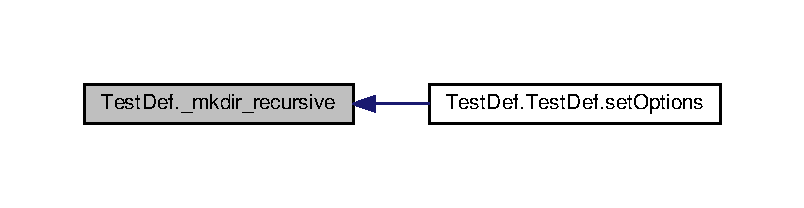
\includegraphics[width=350pt]{namespaceTestDef_a0f44619ec0fe932324e50d8cf706d647_icgraph}
\end{center}
\end{figure}




\subsection{Variable Documentation}
\hypertarget{namespaceTestDef_a4e87724b7a6a117c2cca22c557936868}{\index{Test\-Def@{Test\-Def}!is\-\_\-py2@{is\-\_\-py2}}
\index{is\-\_\-py2@{is\-\_\-py2}!TestDef@{Test\-Def}}
\subsubsection[{is\-\_\-py2}]{\setlength{\rightskip}{0pt plus 5cm}list Test\-Def.\-is\-\_\-py2 = sys.\-version\mbox{[}0\mbox{]}}}\label{namespaceTestDef_a4e87724b7a6a117c2cca22c557936868}


Definition at line 29 of file Test\-Def.\-py.


\hypertarget{namespaceTestGetMTTStage}{\section{Test\-Get\-M\-T\-T\-Stage Namespace Reference}
\label{namespaceTestGetMTTStage}\index{Test\-Get\-M\-T\-T\-Stage@{Test\-Get\-M\-T\-T\-Stage}}
}
\subsection*{Classes}
\begin{DoxyCompactItemize}
\item 
class \hyperlink{classTestGetMTTStage_1_1TestGetMTTStage}{Test\-Get\-M\-T\-T\-Stage}
\end{DoxyCompactItemize}

\hypertarget{namespaceTestRunMTTStage}{\section{Test\-Run\-M\-T\-T\-Stage Namespace Reference}
\label{namespaceTestRunMTTStage}\index{Test\-Run\-M\-T\-T\-Stage@{Test\-Run\-M\-T\-T\-Stage}}
}
\subsection*{Classes}
\begin{DoxyCompactItemize}
\item 
class \hyperlink{classTestRunMTTStage_1_1TestRunMTTStage}{Test\-Run\-M\-T\-T\-Stage}
\end{DoxyCompactItemize}

\hypertarget{namespaceTextFile}{\section{Text\-File Namespace Reference}
\label{namespaceTextFile}\index{Text\-File@{Text\-File}}
}

\hypertarget{namespacetrivial}{\section{trivial Namespace Reference}
\label{namespacetrivial}\index{trivial@{trivial}}
}
\subsection*{Variables}
\begin{DoxyCompactItemize}
\item 
\hyperlink{namespacetrivial_a3e713ea5d6e77bf165eeaafc02275430}{module} = Trivial
\item 
\hyperlink{namespacetrivial_afe75cace659f04749ee3f7c818152b7b}{test\-\_\-get} = trivial
\item 
int \hyperlink{namespacetrivial_af272dc5ab194f706f77eeb74de7b8c97}{save\-\_\-stdout\-\_\-on\-\_\-success} = 1
\item 
int \hyperlink{namespacetrivial_a8c1d5357654e053cf4d0b8a7f48ff13b}{merge\-\_\-stdout\-\_\-stderr} = 1
\item 
int \hyperlink{namespacetrivial_af6ee4456e84c354e7845aae7ea24d022}{stderr\-\_\-save\-\_\-lines} = 100
\item 
\hyperlink{namespacetrivial_aa612b0f8daffd666959f885b6ba54cd0}{test\-\_\-build} = trivial
\item 
tuple \hyperlink{namespacetrivial_a65b4003f52ce4fa5d324695f54c1e3b3}{pass} = \&and(\&cmd\-\_\-wifexited(), \&eq(\&cmd\-\_\-wexitstatus(), 0))
\item 
tuple \hyperlink{namespacetrivial_a8ce5c7e487f1c21edda391cc47830f5e}{timeout} = \&test\-\_\-np()
\item 
int \hyperlink{namespacetrivial_aefbe39eb9fcb8a58d4e04dd980e35062}{save\-\_\-stdout\-\_\-on\-\_\-pass} = 1
\item 
int \hyperlink{namespacetrivial_aee208868790b8c2d6d9f48ad238aa6c5}{stdout\-\_\-save\-\_\-lines} = 100
\item 
tuple \hyperlink{namespacetrivial_adfe4da0e2d8f3078b198c0f76ee394dd}{np} = \&env\-\_\-max\-\_\-procs()
\item 
\hyperlink{namespacetrivial_af5dae1522345f303cfb4527587cd5361}{specify\-\_\-module} = Simple
\end{DoxyCompactItemize}


\subsection{Variable Documentation}
\hypertarget{namespacetrivial_a8c1d5357654e053cf4d0b8a7f48ff13b}{\index{trivial@{trivial}!merge\-\_\-stdout\-\_\-stderr@{merge\-\_\-stdout\-\_\-stderr}}
\index{merge\-\_\-stdout\-\_\-stderr@{merge\-\_\-stdout\-\_\-stderr}!trivial@{trivial}}
\subsubsection[{merge\-\_\-stdout\-\_\-stderr}]{\setlength{\rightskip}{0pt plus 5cm}int trivial.\-merge\-\_\-stdout\-\_\-stderr = 1}}\label{namespacetrivial_a8c1d5357654e053cf4d0b8a7f48ff13b}


Definition at line 21 of file trivial.\-ini.

\hypertarget{namespacetrivial_a3e713ea5d6e77bf165eeaafc02275430}{\index{trivial@{trivial}!module@{module}}
\index{module@{module}!trivial@{trivial}}
\subsubsection[{module}]{\setlength{\rightskip}{0pt plus 5cm}trivial.\-module = Trivial}}\label{namespacetrivial_a3e713ea5d6e77bf165eeaafc02275430}


Definition at line 14 of file trivial.\-ini.

\hypertarget{namespacetrivial_adfe4da0e2d8f3078b198c0f76ee394dd}{\index{trivial@{trivial}!np@{np}}
\index{np@{np}!trivial@{trivial}}
\subsubsection[{np}]{\setlength{\rightskip}{0pt plus 5cm}tuple trivial.\-np = \&env\-\_\-max\-\_\-procs()}}\label{namespacetrivial_adfe4da0e2d8f3078b198c0f76ee394dd}


Definition at line 35 of file trivial.\-ini.

\hypertarget{namespacetrivial_a65b4003f52ce4fa5d324695f54c1e3b3}{\index{trivial@{trivial}!pass@{pass}}
\index{pass@{pass}!trivial@{trivial}}
\subsubsection[{pass}]{\setlength{\rightskip}{0pt plus 5cm}tuple trivial.\-pass = \&and(\&cmd\-\_\-wifexited(), \&eq(\&cmd\-\_\-wexitstatus(), 0))}}\label{namespacetrivial_a65b4003f52ce4fa5d324695f54c1e3b3}


Definition at line 30 of file trivial.\-ini.

\hypertarget{namespacetrivial_aefbe39eb9fcb8a58d4e04dd980e35062}{\index{trivial@{trivial}!save\-\_\-stdout\-\_\-on\-\_\-pass@{save\-\_\-stdout\-\_\-on\-\_\-pass}}
\index{save\-\_\-stdout\-\_\-on\-\_\-pass@{save\-\_\-stdout\-\_\-on\-\_\-pass}!trivial@{trivial}}
\subsubsection[{save\-\_\-stdout\-\_\-on\-\_\-pass}]{\setlength{\rightskip}{0pt plus 5cm}int trivial.\-save\-\_\-stdout\-\_\-on\-\_\-pass = 1}}\label{namespacetrivial_aefbe39eb9fcb8a58d4e04dd980e35062}


Definition at line 32 of file trivial.\-ini.

\hypertarget{namespacetrivial_af272dc5ab194f706f77eeb74de7b8c97}{\index{trivial@{trivial}!save\-\_\-stdout\-\_\-on\-\_\-success@{save\-\_\-stdout\-\_\-on\-\_\-success}}
\index{save\-\_\-stdout\-\_\-on\-\_\-success@{save\-\_\-stdout\-\_\-on\-\_\-success}!trivial@{trivial}}
\subsubsection[{save\-\_\-stdout\-\_\-on\-\_\-success}]{\setlength{\rightskip}{0pt plus 5cm}int trivial.\-save\-\_\-stdout\-\_\-on\-\_\-success = 1}}\label{namespacetrivial_af272dc5ab194f706f77eeb74de7b8c97}


Definition at line 20 of file trivial.\-ini.

\hypertarget{namespacetrivial_af5dae1522345f303cfb4527587cd5361}{\index{trivial@{trivial}!specify\-\_\-module@{specify\-\_\-module}}
\index{specify\-\_\-module@{specify\-\_\-module}!trivial@{trivial}}
\subsubsection[{specify\-\_\-module}]{\setlength{\rightskip}{0pt plus 5cm}trivial.\-specify\-\_\-module = Simple}}\label{namespacetrivial_af5dae1522345f303cfb4527587cd5361}


Definition at line 37 of file trivial.\-ini.

\hypertarget{namespacetrivial_af6ee4456e84c354e7845aae7ea24d022}{\index{trivial@{trivial}!stderr\-\_\-save\-\_\-lines@{stderr\-\_\-save\-\_\-lines}}
\index{stderr\-\_\-save\-\_\-lines@{stderr\-\_\-save\-\_\-lines}!trivial@{trivial}}
\subsubsection[{stderr\-\_\-save\-\_\-lines}]{\setlength{\rightskip}{0pt plus 5cm}int trivial.\-stderr\-\_\-save\-\_\-lines = 100}}\label{namespacetrivial_af6ee4456e84c354e7845aae7ea24d022}


Definition at line 22 of file trivial.\-ini.

\hypertarget{namespacetrivial_aee208868790b8c2d6d9f48ad238aa6c5}{\index{trivial@{trivial}!stdout\-\_\-save\-\_\-lines@{stdout\-\_\-save\-\_\-lines}}
\index{stdout\-\_\-save\-\_\-lines@{stdout\-\_\-save\-\_\-lines}!trivial@{trivial}}
\subsubsection[{stdout\-\_\-save\-\_\-lines}]{\setlength{\rightskip}{0pt plus 5cm}int trivial.\-stdout\-\_\-save\-\_\-lines = 100}}\label{namespacetrivial_aee208868790b8c2d6d9f48ad238aa6c5}


Definition at line 34 of file trivial.\-ini.

\hypertarget{namespacetrivial_aa612b0f8daffd666959f885b6ba54cd0}{\index{trivial@{trivial}!test\-\_\-build@{test\-\_\-build}}
\index{test\-\_\-build@{test\-\_\-build}!trivial@{trivial}}
\subsubsection[{test\-\_\-build}]{\setlength{\rightskip}{0pt plus 5cm}trivial.\-test\-\_\-build = trivial}}\label{namespacetrivial_aa612b0f8daffd666959f885b6ba54cd0}


Definition at line 29 of file trivial.\-ini.

\hypertarget{namespacetrivial_afe75cace659f04749ee3f7c818152b7b}{\index{trivial@{trivial}!test\-\_\-get@{test\-\_\-get}}
\index{test\-\_\-get@{test\-\_\-get}!trivial@{trivial}}
\subsubsection[{test\-\_\-get}]{\setlength{\rightskip}{0pt plus 5cm}trivial.\-test\-\_\-get = trivial}}\label{namespacetrivial_afe75cace659f04749ee3f7c818152b7b}


Definition at line 19 of file trivial.\-ini.

\hypertarget{namespacetrivial_a8ce5c7e487f1c21edda391cc47830f5e}{\index{trivial@{trivial}!timeout@{timeout}}
\index{timeout@{timeout}!trivial@{trivial}}
\subsubsection[{timeout}]{\setlength{\rightskip}{0pt plus 5cm}tuple trivial.\-timeout = \&test\-\_\-np()}}\label{namespacetrivial_a8ce5c7e487f1c21edda391cc47830f5e}


Definition at line 31 of file trivial.\-ini.


\hypertarget{namespaceVersionMTTTool}{\section{Version\-M\-T\-T\-Tool Namespace Reference}
\label{namespaceVersionMTTTool}\index{Version\-M\-T\-T\-Tool@{Version\-M\-T\-T\-Tool}}
}

\hypertarget{namespaceWatchdog}{\section{Watchdog Namespace Reference}
\label{namespaceWatchdog}\index{Watchdog@{Watchdog}}
}

\hypertarget{namespaceWWulf3}{\section{W\-Wulf3 Namespace Reference}
\label{namespaceWWulf3}\index{W\-Wulf3@{W\-Wulf3}}
}

\chapter{File Documentation}
\hypertarget{pymtt_8py}{\section{/home/travis/build/\-Jagaskak/mtt/pyclient/pymtt.py File Reference}
\label{pymtt_8py}\index{/home/travis/build/\-Jagaskak/mtt/pyclient/pymtt.\-py@{/home/travis/build/\-Jagaskak/mtt/pyclient/pymtt.\-py}}
}
\subsection*{Namespaces}
\begin{DoxyCompactItemize}
\item 
\hyperlink{namespacepymtt}{pymtt}
\end{DoxyCompactItemize}

\hypertarget{BIOSMTTStage_8py}{\section{/home/travis/build/\-Jagaskak/mtt/pylib/\-Stages/\-B\-I\-O\-S/\-B\-I\-O\-S\-M\-T\-T\-Stage.py File Reference}
\label{BIOSMTTStage_8py}\index{/home/travis/build/\-Jagaskak/mtt/pylib/\-Stages/\-B\-I\-O\-S/\-B\-I\-O\-S\-M\-T\-T\-Stage.\-py@{/home/travis/build/\-Jagaskak/mtt/pylib/\-Stages/\-B\-I\-O\-S/\-B\-I\-O\-S\-M\-T\-T\-Stage.\-py}}
}
\subsection*{Classes}
\begin{DoxyCompactItemize}
\item 
class \hyperlink{classBIOSMTTStage_1_1BIOSMTTStage}{B\-I\-O\-S\-M\-T\-T\-Stage.\-B\-I\-O\-S\-M\-T\-T\-Stage}
\end{DoxyCompactItemize}
\subsection*{Namespaces}
\begin{DoxyCompactItemize}
\item 
\hyperlink{namespaceBIOSMTTStage}{B\-I\-O\-S\-M\-T\-T\-Stage}
\end{DoxyCompactItemize}

\hypertarget{FirmwareMTTStage_8py}{\section{/home/travis/build/\-Jagaskak/mtt/pylib/\-Stages/\-Firmware/\-Firmware\-M\-T\-T\-Stage.py File Reference}
\label{FirmwareMTTStage_8py}\index{/home/travis/build/\-Jagaskak/mtt/pylib/\-Stages/\-Firmware/\-Firmware\-M\-T\-T\-Stage.\-py@{/home/travis/build/\-Jagaskak/mtt/pylib/\-Stages/\-Firmware/\-Firmware\-M\-T\-T\-Stage.\-py}}
}
\subsection*{Classes}
\begin{DoxyCompactItemize}
\item 
class \hyperlink{classFirmwareMTTStage_1_1FirmwareMTTStage}{Firmware\-M\-T\-T\-Stage.\-Firmware\-M\-T\-T\-Stage}
\end{DoxyCompactItemize}
\subsection*{Namespaces}
\begin{DoxyCompactItemize}
\item 
\hyperlink{namespaceFirmwareMTTStage}{Firmware\-M\-T\-T\-Stage}
\end{DoxyCompactItemize}

\hypertarget{FooFlash_8py}{\section{/home/travis/build/\-Jagaskak/mtt/pylib/\-Stages/\-Firmware/\-Foo\-Flash.py File Reference}
\label{FooFlash_8py}\index{/home/travis/build/\-Jagaskak/mtt/pylib/\-Stages/\-Firmware/\-Foo\-Flash.\-py@{/home/travis/build/\-Jagaskak/mtt/pylib/\-Stages/\-Firmware/\-Foo\-Flash.\-py}}
}
\subsection*{Classes}
\begin{DoxyCompactItemize}
\item 
class \hyperlink{classFooFlash_1_1FooFlash}{Foo\-Flash.\-Foo\-Flash}
\end{DoxyCompactItemize}
\subsection*{Namespaces}
\begin{DoxyCompactItemize}
\item 
\hyperlink{namespaceFooFlash}{Foo\-Flash}
\end{DoxyCompactItemize}

\hypertarget{LauncherDefaultsMTTStage_8py}{\section{/home/travis/build/\-Jagaskak/mtt/pylib/\-Stages/\-Launcher\-Defaults/\-Launcher\-Defaults\-M\-T\-T\-Stage.py File Reference}
\label{LauncherDefaultsMTTStage_8py}\index{/home/travis/build/\-Jagaskak/mtt/pylib/\-Stages/\-Launcher\-Defaults/\-Launcher\-Defaults\-M\-T\-T\-Stage.\-py@{/home/travis/build/\-Jagaskak/mtt/pylib/\-Stages/\-Launcher\-Defaults/\-Launcher\-Defaults\-M\-T\-T\-Stage.\-py}}
}
\subsection*{Namespaces}
\begin{DoxyCompactItemize}
\item 
\hyperlink{namespaceLauncherDefaultsMTTStage}{Launcher\-Defaults\-M\-T\-T\-Stage}
\end{DoxyCompactItemize}

\hypertarget{MiddlewareBuildMTTStage_8py}{\section{/home/travis/build/\-Jagaskak/mtt/pylib/\-Stages/\-Middleware\-Build/\-Middleware\-Build\-M\-T\-T\-Stage.py File Reference}
\label{MiddlewareBuildMTTStage_8py}\index{/home/travis/build/\-Jagaskak/mtt/pylib/\-Stages/\-Middleware\-Build/\-Middleware\-Build\-M\-T\-T\-Stage.\-py@{/home/travis/build/\-Jagaskak/mtt/pylib/\-Stages/\-Middleware\-Build/\-Middleware\-Build\-M\-T\-T\-Stage.\-py}}
}
\subsection*{Classes}
\begin{DoxyCompactItemize}
\item 
class \hyperlink{classMiddlewareBuildMTTStage_1_1MiddlewareBuildMTTStage}{Middleware\-Build\-M\-T\-T\-Stage.\-Middleware\-Build\-M\-T\-T\-Stage}
\end{DoxyCompactItemize}
\subsection*{Namespaces}
\begin{DoxyCompactItemize}
\item 
\hyperlink{namespaceMiddlewareBuildMTTStage}{Middleware\-Build\-M\-T\-T\-Stage}
\end{DoxyCompactItemize}

\hypertarget{MiddlewareGetMTTStage_8py}{\section{/home/travis/build/\-Jagaskak/mtt/pylib/\-Stages/\-Middleware\-Get/\-Middleware\-Get\-M\-T\-T\-Stage.py File Reference}
\label{MiddlewareGetMTTStage_8py}\index{/home/travis/build/\-Jagaskak/mtt/pylib/\-Stages/\-Middleware\-Get/\-Middleware\-Get\-M\-T\-T\-Stage.\-py@{/home/travis/build/\-Jagaskak/mtt/pylib/\-Stages/\-Middleware\-Get/\-Middleware\-Get\-M\-T\-T\-Stage.\-py}}
}
\subsection*{Namespaces}
\begin{DoxyCompactItemize}
\item 
\hyperlink{namespaceMiddlewareGetMTTStage}{Middleware\-Get\-M\-T\-T\-Stage}
\end{DoxyCompactItemize}

\hypertarget{DefaultMTTDefaults_8py}{\section{/home/travis/build/\-Jagaskak/mtt/pylib/\-Stages/\-M\-T\-T\-Defaults/\-Default\-M\-T\-T\-Defaults.py File Reference}
\label{DefaultMTTDefaults_8py}\index{/home/travis/build/\-Jagaskak/mtt/pylib/\-Stages/\-M\-T\-T\-Defaults/\-Default\-M\-T\-T\-Defaults.\-py@{/home/travis/build/\-Jagaskak/mtt/pylib/\-Stages/\-M\-T\-T\-Defaults/\-Default\-M\-T\-T\-Defaults.\-py}}
}
\subsection*{Namespaces}
\begin{DoxyCompactItemize}
\item 
\hyperlink{namespaceDefaultMTTDefaults}{Default\-M\-T\-T\-Defaults}
\end{DoxyCompactItemize}

\hypertarget{MTTDefaultsMTTStage_8py}{\section{/home/travis/build/\-Jagaskak/mtt/pylib/\-Stages/\-M\-T\-T\-Defaults/\-M\-T\-T\-Defaults\-M\-T\-T\-Stage.py File Reference}
\label{MTTDefaultsMTTStage_8py}\index{/home/travis/build/\-Jagaskak/mtt/pylib/\-Stages/\-M\-T\-T\-Defaults/\-M\-T\-T\-Defaults\-M\-T\-T\-Stage.\-py@{/home/travis/build/\-Jagaskak/mtt/pylib/\-Stages/\-M\-T\-T\-Defaults/\-M\-T\-T\-Defaults\-M\-T\-T\-Stage.\-py}}
}
\subsection*{Namespaces}
\begin{DoxyCompactItemize}
\item 
\hyperlink{namespaceMTTDefaultsMTTStage}{M\-T\-T\-Defaults\-M\-T\-T\-Stage}
\end{DoxyCompactItemize}

\hypertarget{DefaultProfile_8py}{\section{/home/travis/build/\-Jagaskak/mtt/pylib/\-Stages/\-Profile/\-Default\-Profile.py File Reference}
\label{DefaultProfile_8py}\index{/home/travis/build/\-Jagaskak/mtt/pylib/\-Stages/\-Profile/\-Default\-Profile.\-py@{/home/travis/build/\-Jagaskak/mtt/pylib/\-Stages/\-Profile/\-Default\-Profile.\-py}}
}
\subsection*{Namespaces}
\begin{DoxyCompactItemize}
\item 
\hyperlink{namespaceDefaultProfile}{Default\-Profile}
\end{DoxyCompactItemize}

\hypertarget{ProfileMTTStage_8py}{\section{/home/travis/build/\-Jagaskak/mtt/pylib/\-Stages/\-Profile/\-Profile\-M\-T\-T\-Stage.py File Reference}
\label{ProfileMTTStage_8py}\index{/home/travis/build/\-Jagaskak/mtt/pylib/\-Stages/\-Profile/\-Profile\-M\-T\-T\-Stage.\-py@{/home/travis/build/\-Jagaskak/mtt/pylib/\-Stages/\-Profile/\-Profile\-M\-T\-T\-Stage.\-py}}
}
\subsection*{Classes}
\begin{DoxyCompactItemize}
\item 
class \hyperlink{classProfileMTTStage_1_1ProfileMTTStage}{Profile\-M\-T\-T\-Stage.\-Profile\-M\-T\-T\-Stage}
\end{DoxyCompactItemize}
\subsection*{Namespaces}
\begin{DoxyCompactItemize}
\item 
\hyperlink{namespaceProfileMTTStage}{Profile\-M\-T\-T\-Stage}
\end{DoxyCompactItemize}

\hypertarget{ProvisionMTTStage_8py}{\section{/home/travis/build/\-Jagaskak/mtt/pylib/\-Stages/\-Provisioning/\-Provision\-M\-T\-T\-Stage.py File Reference}
\label{ProvisionMTTStage_8py}\index{/home/travis/build/\-Jagaskak/mtt/pylib/\-Stages/\-Provisioning/\-Provision\-M\-T\-T\-Stage.\-py@{/home/travis/build/\-Jagaskak/mtt/pylib/\-Stages/\-Provisioning/\-Provision\-M\-T\-T\-Stage.\-py}}
}
\subsection*{Classes}
\begin{DoxyCompactItemize}
\item 
class \hyperlink{classProvisionMTTStage_1_1ProvisionMTTStage}{Provision\-M\-T\-T\-Stage.\-Provision\-M\-T\-T\-Stage}
\end{DoxyCompactItemize}
\subsection*{Namespaces}
\begin{DoxyCompactItemize}
\item 
\hyperlink{namespaceProvisionMTTStage}{Provision\-M\-T\-T\-Stage}
\end{DoxyCompactItemize}

\hypertarget{WWulf3_8py}{\section{/home/travis/build/\-Jagaskak/mtt/pylib/\-Stages/\-Provisioning/\-W\-Wulf3.py File Reference}
\label{WWulf3_8py}\index{/home/travis/build/\-Jagaskak/mtt/pylib/\-Stages/\-Provisioning/\-W\-Wulf3.\-py@{/home/travis/build/\-Jagaskak/mtt/pylib/\-Stages/\-Provisioning/\-W\-Wulf3.\-py}}
}
\subsection*{Classes}
\begin{DoxyCompactItemize}
\item 
class \hyperlink{classWWulf3_1_1WWulf3}{W\-Wulf3.\-W\-Wulf3}
\end{DoxyCompactItemize}
\subsection*{Namespaces}
\begin{DoxyCompactItemize}
\item 
\hyperlink{namespaceWWulf3}{W\-Wulf3}
\end{DoxyCompactItemize}

\hypertarget{IUDatabase_8py}{\section{/home/travis/build/\-Jagaskak/mtt/pylib/\-Stages/\-Reporter/\-I\-U\-Database.py File Reference}
\label{IUDatabase_8py}\index{/home/travis/build/\-Jagaskak/mtt/pylib/\-Stages/\-Reporter/\-I\-U\-Database.\-py@{/home/travis/build/\-Jagaskak/mtt/pylib/\-Stages/\-Reporter/\-I\-U\-Database.\-py}}
}
\subsection*{Classes}
\begin{DoxyCompactItemize}
\item 
class \hyperlink{classIUDatabase_1_1IUDatabase}{I\-U\-Database.\-I\-U\-Database}
\end{DoxyCompactItemize}
\subsection*{Namespaces}
\begin{DoxyCompactItemize}
\item 
\hyperlink{namespaceIUDatabase}{I\-U\-Database}
\end{DoxyCompactItemize}

\hypertarget{JunitXML_8py}{\section{/home/travis/build/\-Jagaskak/mtt/pylib/\-Stages/\-Reporter/\-Junit\-X\-M\-L.py File Reference}
\label{JunitXML_8py}\index{/home/travis/build/\-Jagaskak/mtt/pylib/\-Stages/\-Reporter/\-Junit\-X\-M\-L.\-py@{/home/travis/build/\-Jagaskak/mtt/pylib/\-Stages/\-Reporter/\-Junit\-X\-M\-L.\-py}}
}
\subsection*{Classes}
\begin{DoxyCompactItemize}
\item 
class \hyperlink{classJunitXML_1_1JunitXML}{Junit\-X\-M\-L.\-Junit\-X\-M\-L}
\end{DoxyCompactItemize}
\subsection*{Namespaces}
\begin{DoxyCompactItemize}
\item 
\hyperlink{namespaceJunitXML}{Junit\-X\-M\-L}
\end{DoxyCompactItemize}

\hypertarget{ReporterMTTStage_8py}{\section{/home/travis/build/\-Jagaskak/mtt/pylib/\-Stages/\-Reporter/\-Reporter\-M\-T\-T\-Stage.py File Reference}
\label{ReporterMTTStage_8py}\index{/home/travis/build/\-Jagaskak/mtt/pylib/\-Stages/\-Reporter/\-Reporter\-M\-T\-T\-Stage.\-py@{/home/travis/build/\-Jagaskak/mtt/pylib/\-Stages/\-Reporter/\-Reporter\-M\-T\-T\-Stage.\-py}}
}
\subsection*{Classes}
\begin{DoxyCompactItemize}
\item 
class \hyperlink{classReporterMTTStage_1_1ReporterMTTStage}{Reporter\-M\-T\-T\-Stage.\-Reporter\-M\-T\-T\-Stage}
\end{DoxyCompactItemize}
\subsection*{Namespaces}
\begin{DoxyCompactItemize}
\item 
\hyperlink{namespaceReporterMTTStage}{Reporter\-M\-T\-T\-Stage}
\end{DoxyCompactItemize}

\hypertarget{TextFile_8py}{\section{/home/travis/build/\-Jagaskak/mtt/pylib/\-Stages/\-Reporter/\-Text\-File.py File Reference}
\label{TextFile_8py}\index{/home/travis/build/\-Jagaskak/mtt/pylib/\-Stages/\-Reporter/\-Text\-File.\-py@{/home/travis/build/\-Jagaskak/mtt/pylib/\-Stages/\-Reporter/\-Text\-File.\-py}}
}
\subsection*{Namespaces}
\begin{DoxyCompactItemize}
\item 
\hyperlink{namespaceTextFile}{Text\-File}
\end{DoxyCompactItemize}

\hypertarget{DefaultTestBuild_8py}{\section{/home/travis/build/\-Jagaskak/mtt/pylib/\-Stages/\-Test\-Build/\-Default\-Test\-Build.py File Reference}
\label{DefaultTestBuild_8py}\index{/home/travis/build/\-Jagaskak/mtt/pylib/\-Stages/\-Test\-Build/\-Default\-Test\-Build.\-py@{/home/travis/build/\-Jagaskak/mtt/pylib/\-Stages/\-Test\-Build/\-Default\-Test\-Build.\-py}}
}
\subsection*{Namespaces}
\begin{DoxyCompactItemize}
\item 
\hyperlink{namespaceDefaultTestBuild}{Default\-Test\-Build}
\end{DoxyCompactItemize}

\hypertarget{TestBuildMTTStage_8py}{\section{/home/travis/build/\-Jagaskak/mtt/pylib/\-Stages/\-Test\-Build/\-Test\-Build\-M\-T\-T\-Stage.py File Reference}
\label{TestBuildMTTStage_8py}\index{/home/travis/build/\-Jagaskak/mtt/pylib/\-Stages/\-Test\-Build/\-Test\-Build\-M\-T\-T\-Stage.\-py@{/home/travis/build/\-Jagaskak/mtt/pylib/\-Stages/\-Test\-Build/\-Test\-Build\-M\-T\-T\-Stage.\-py}}
}
\subsection*{Classes}
\begin{DoxyCompactItemize}
\item 
class \hyperlink{classTestBuildMTTStage_1_1TestBuildMTTStage}{Test\-Build\-M\-T\-T\-Stage.\-Test\-Build\-M\-T\-T\-Stage}
\end{DoxyCompactItemize}
\subsection*{Namespaces}
\begin{DoxyCompactItemize}
\item 
\hyperlink{namespaceTestBuildMTTStage}{Test\-Build\-M\-T\-T\-Stage}
\end{DoxyCompactItemize}

\hypertarget{TestGetMTTStage_8py}{\section{/home/travis/build/\-Jagaskak/mtt/pylib/\-Stages/\-Test\-Get/\-Test\-Get\-M\-T\-T\-Stage.py File Reference}
\label{TestGetMTTStage_8py}\index{/home/travis/build/\-Jagaskak/mtt/pylib/\-Stages/\-Test\-Get/\-Test\-Get\-M\-T\-T\-Stage.\-py@{/home/travis/build/\-Jagaskak/mtt/pylib/\-Stages/\-Test\-Get/\-Test\-Get\-M\-T\-T\-Stage.\-py}}
}
\subsection*{Namespaces}
\begin{DoxyCompactItemize}
\item 
\hyperlink{namespaceTestGetMTTStage}{Test\-Get\-M\-T\-T\-Stage}
\end{DoxyCompactItemize}

\hypertarget{TestRunMTTStage_8py}{\section{/home/travis/build/\-Jagaskak/mtt/pylib/\-Stages/\-Test\-Run/\-Test\-Run\-M\-T\-T\-Stage.py File Reference}
\label{TestRunMTTStage_8py}\index{/home/travis/build/\-Jagaskak/mtt/pylib/\-Stages/\-Test\-Run/\-Test\-Run\-M\-T\-T\-Stage.\-py@{/home/travis/build/\-Jagaskak/mtt/pylib/\-Stages/\-Test\-Run/\-Test\-Run\-M\-T\-T\-Stage.\-py}}
}
\subsection*{Classes}
\begin{DoxyCompactItemize}
\item 
class \hyperlink{classTestRunMTTStage_1_1TestRunMTTStage}{Test\-Run\-M\-T\-T\-Stage.\-Test\-Run\-M\-T\-T\-Stage}
\end{DoxyCompactItemize}
\subsection*{Namespaces}
\begin{DoxyCompactItemize}
\item 
\hyperlink{namespaceTestRunMTTStage}{Test\-Run\-M\-T\-T\-Stage}
\end{DoxyCompactItemize}

\hypertarget{LoadClasses_8py}{\section{/home/travis/build/\-Jagaskak/mtt/pylib/\-System/\-Load\-Classes.py File Reference}
\label{LoadClasses_8py}\index{/home/travis/build/\-Jagaskak/mtt/pylib/\-System/\-Load\-Classes.\-py@{/home/travis/build/\-Jagaskak/mtt/pylib/\-System/\-Load\-Classes.\-py}}
}
\subsection*{Classes}
\begin{DoxyCompactItemize}
\item 
class \hyperlink{classLoadClasses_1_1LoadClasses}{Load\-Classes.\-Load\-Classes}
\end{DoxyCompactItemize}
\subsection*{Namespaces}
\begin{DoxyCompactItemize}
\item 
\hyperlink{namespaceLoadClasses}{Load\-Classes}
\end{DoxyCompactItemize}

\hypertarget{TestDef_8py}{\section{/home/travis/build/\-Jagaskak/mtt/pylib/\-System/\-Test\-Def.py File Reference}
\label{TestDef_8py}\index{/home/travis/build/\-Jagaskak/mtt/pylib/\-System/\-Test\-Def.\-py@{/home/travis/build/\-Jagaskak/mtt/pylib/\-System/\-Test\-Def.\-py}}
}
\subsection*{Namespaces}
\begin{DoxyCompactItemize}
\item 
\hyperlink{namespaceTestDef}{Test\-Def}
\end{DoxyCompactItemize}

\hypertarget{Autotools_8py}{\section{/home/travis/build/\-Jagaskak/mtt/pylib/\-Tools/\-Build/\-Autotools.py File Reference}
\label{Autotools_8py}\index{/home/travis/build/\-Jagaskak/mtt/pylib/\-Tools/\-Build/\-Autotools.\-py@{/home/travis/build/\-Jagaskak/mtt/pylib/\-Tools/\-Build/\-Autotools.\-py}}
}
\subsection*{Classes}
\begin{DoxyCompactItemize}
\item 
class \hyperlink{classAutotools_1_1Autotools}{Autotools.\-Autotools}
\end{DoxyCompactItemize}
\subsection*{Namespaces}
\begin{DoxyCompactItemize}
\item 
\hyperlink{namespaceAutotools}{Autotools}
\end{DoxyCompactItemize}

\hypertarget{BuildMTTTool_8py}{\section{/home/travis/build/\-Jagaskak/mtt/pylib/\-Tools/\-Build/\-Build\-M\-T\-T\-Tool.py File Reference}
\label{BuildMTTTool_8py}\index{/home/travis/build/\-Jagaskak/mtt/pylib/\-Tools/\-Build/\-Build\-M\-T\-T\-Tool.\-py@{/home/travis/build/\-Jagaskak/mtt/pylib/\-Tools/\-Build/\-Build\-M\-T\-T\-Tool.\-py}}
}
\subsection*{Classes}
\begin{DoxyCompactItemize}
\item 
class \hyperlink{classBuildMTTTool_1_1BuildMTTTool}{Build\-M\-T\-T\-Tool.\-Build\-M\-T\-T\-Tool}
\end{DoxyCompactItemize}
\subsection*{Namespaces}
\begin{DoxyCompactItemize}
\item 
\hyperlink{namespaceBuildMTTTool}{Build\-M\-T\-T\-Tool}
\end{DoxyCompactItemize}

\hypertarget{Hostfile_8py}{\section{/home/travis/build/\-Jagaskak/mtt/pylib/\-Tools/\-Build/\-Hostfile.py File Reference}
\label{Hostfile_8py}\index{/home/travis/build/\-Jagaskak/mtt/pylib/\-Tools/\-Build/\-Hostfile.\-py@{/home/travis/build/\-Jagaskak/mtt/pylib/\-Tools/\-Build/\-Hostfile.\-py}}
}
\subsection*{Namespaces}
\begin{DoxyCompactItemize}
\item 
\hyperlink{namespaceHostfile}{Hostfile}
\end{DoxyCompactItemize}

\hypertarget{Shell_8py}{\section{/home/travis/build/\-Jagaskak/mtt/pylib/\-Tools/\-Build/\-Shell.py File Reference}
\label{Shell_8py}\index{/home/travis/build/\-Jagaskak/mtt/pylib/\-Tools/\-Build/\-Shell.\-py@{/home/travis/build/\-Jagaskak/mtt/pylib/\-Tools/\-Build/\-Shell.\-py}}
}
\subsection*{Namespaces}
\begin{DoxyCompactItemize}
\item 
\hyperlink{namespaceShell}{Shell}
\end{DoxyCompactItemize}

\hypertarget{CNCMTTTool_8py}{\section{/home/travis/build/\-Jagaskak/mtt/pylib/\-Tools/\-C\-N\-C/\-C\-N\-C\-M\-T\-T\-Tool.py File Reference}
\label{CNCMTTTool_8py}\index{/home/travis/build/\-Jagaskak/mtt/pylib/\-Tools/\-C\-N\-C/\-C\-N\-C\-M\-T\-T\-Tool.\-py@{/home/travis/build/\-Jagaskak/mtt/pylib/\-Tools/\-C\-N\-C/\-C\-N\-C\-M\-T\-T\-Tool.\-py}}
}
\subsection*{Namespaces}
\begin{DoxyCompactItemize}
\item 
\hyperlink{namespaceCNCMTTTool}{C\-N\-C\-M\-T\-T\-Tool}
\end{DoxyCompactItemize}

\hypertarget{IPMITool_8py}{\section{/home/travis/build/\-Jagaskak/mtt/pylib/\-Tools/\-C\-N\-C/\-I\-P\-M\-I\-Tool.py File Reference}
\label{IPMITool_8py}\index{/home/travis/build/\-Jagaskak/mtt/pylib/\-Tools/\-C\-N\-C/\-I\-P\-M\-I\-Tool.\-py@{/home/travis/build/\-Jagaskak/mtt/pylib/\-Tools/\-C\-N\-C/\-I\-P\-M\-I\-Tool.\-py}}
}
\subsection*{Classes}
\begin{DoxyCompactItemize}
\item 
class \hyperlink{classIPMITool_1_1workerThread}{I\-P\-M\-I\-Tool.\-worker\-Thread}
\item 
class \hyperlink{classIPMITool_1_1IPMITool}{I\-P\-M\-I\-Tool.\-I\-P\-M\-I\-Tool}
\end{DoxyCompactItemize}
\subsection*{Namespaces}
\begin{DoxyCompactItemize}
\item 
\hyperlink{namespaceIPMITool}{I\-P\-M\-I\-Tool}
\end{DoxyCompactItemize}

\hypertarget{combinatorial_8py}{\section{/home/travis/build/\-Jagaskak/mtt/pylib/\-Tools/\-Executor/combinatorial.py File Reference}
\label{combinatorial_8py}\index{/home/travis/build/\-Jagaskak/mtt/pylib/\-Tools/\-Executor/combinatorial.\-py@{/home/travis/build/\-Jagaskak/mtt/pylib/\-Tools/\-Executor/combinatorial.\-py}}
}
\subsection*{Classes}
\begin{DoxyCompactItemize}
\item 
class \hyperlink{classcombinatorial_1_1CombinatorialEx}{combinatorial.\-Combinatorial\-Ex}
\end{DoxyCompactItemize}
\subsection*{Namespaces}
\begin{DoxyCompactItemize}
\item 
\hyperlink{namespacecombinatorial}{combinatorial}
\end{DoxyCompactItemize}

\hypertarget{ExecutorMTTTool_8py}{\section{/home/travis/build/\-Jagaskak/mtt/pylib/\-Tools/\-Executor/\-Executor\-M\-T\-T\-Tool.py File Reference}
\label{ExecutorMTTTool_8py}\index{/home/travis/build/\-Jagaskak/mtt/pylib/\-Tools/\-Executor/\-Executor\-M\-T\-T\-Tool.\-py@{/home/travis/build/\-Jagaskak/mtt/pylib/\-Tools/\-Executor/\-Executor\-M\-T\-T\-Tool.\-py}}
}
\subsection*{Classes}
\begin{DoxyCompactItemize}
\item 
class \hyperlink{classExecutorMTTTool_1_1ExecutorMTTTool}{Executor\-M\-T\-T\-Tool.\-Executor\-M\-T\-T\-Tool}
\end{DoxyCompactItemize}
\subsection*{Namespaces}
\begin{DoxyCompactItemize}
\item 
\hyperlink{namespaceExecutorMTTTool}{Executor\-M\-T\-T\-Tool}
\end{DoxyCompactItemize}

\hypertarget{sequential_8py}{\section{/home/travis/build/\-Jagaskak/mtt/pylib/\-Tools/\-Executor/sequential.py File Reference}
\label{sequential_8py}\index{/home/travis/build/\-Jagaskak/mtt/pylib/\-Tools/\-Executor/sequential.\-py@{/home/travis/build/\-Jagaskak/mtt/pylib/\-Tools/\-Executor/sequential.\-py}}
}
\subsection*{Classes}
\begin{DoxyCompactItemize}
\item 
class \hyperlink{classsequential_1_1SequentialEx}{sequential.\-Sequential\-Ex}
\end{DoxyCompactItemize}
\subsection*{Namespaces}
\begin{DoxyCompactItemize}
\item 
\hyperlink{namespacesequential}{sequential}
\end{DoxyCompactItemize}
\subsection*{Variables}
\begin{DoxyCompactItemize}
\item 
\hyperlink{namespacesequential_a2bcf64415a328c57bebc08f7fed9d30c}{sequential.\-basestring} = str
\end{DoxyCompactItemize}

\hypertarget{AlreadyInstalled_8py}{\section{/home/travis/build/\-Jagaskak/mtt/pylib/\-Tools/\-Fetch/\-Already\-Installed.py File Reference}
\label{AlreadyInstalled_8py}\index{/home/travis/build/\-Jagaskak/mtt/pylib/\-Tools/\-Fetch/\-Already\-Installed.\-py@{/home/travis/build/\-Jagaskak/mtt/pylib/\-Tools/\-Fetch/\-Already\-Installed.\-py}}
}
\subsection*{Classes}
\begin{DoxyCompactItemize}
\item 
class \hyperlink{classAlreadyInstalled_1_1AlreadyInstalled}{Already\-Installed.\-Already\-Installed}
\end{DoxyCompactItemize}
\subsection*{Namespaces}
\begin{DoxyCompactItemize}
\item 
\hyperlink{namespaceAlreadyInstalled}{Already\-Installed}
\end{DoxyCompactItemize}

\hypertarget{FetchMTTTool_8py}{\section{/home/travis/build/\-Jagaskak/mtt/pylib/\-Tools/\-Fetch/\-Fetch\-M\-T\-T\-Tool.py File Reference}
\label{FetchMTTTool_8py}\index{/home/travis/build/\-Jagaskak/mtt/pylib/\-Tools/\-Fetch/\-Fetch\-M\-T\-T\-Tool.\-py@{/home/travis/build/\-Jagaskak/mtt/pylib/\-Tools/\-Fetch/\-Fetch\-M\-T\-T\-Tool.\-py}}
}
\subsection*{Classes}
\begin{DoxyCompactItemize}
\item 
class \hyperlink{classFetchMTTTool_1_1FetchMTTTool}{Fetch\-M\-T\-T\-Tool.\-Fetch\-M\-T\-T\-Tool}
\end{DoxyCompactItemize}
\subsection*{Namespaces}
\begin{DoxyCompactItemize}
\item 
\hyperlink{namespaceFetchMTTTool}{Fetch\-M\-T\-T\-Tool}
\end{DoxyCompactItemize}

\hypertarget{Git_8py}{\section{/home/travis/build/\-Jagaskak/mtt/pylib/\-Tools/\-Fetch/\-Git.py File Reference}
\label{Git_8py}\index{/home/travis/build/\-Jagaskak/mtt/pylib/\-Tools/\-Fetch/\-Git.\-py@{/home/travis/build/\-Jagaskak/mtt/pylib/\-Tools/\-Fetch/\-Git.\-py}}
}
\subsection*{Namespaces}
\begin{DoxyCompactItemize}
\item 
\hyperlink{namespaceGit}{Git}
\end{DoxyCompactItemize}

\hypertarget{OMPI__Snapshot_8py}{\section{/home/travis/build/\-Jagaskak/mtt/pylib/\-Tools/\-Fetch/\-O\-M\-P\-I\-\_\-\-Snapshot.py File Reference}
\label{OMPI__Snapshot_8py}\index{/home/travis/build/\-Jagaskak/mtt/pylib/\-Tools/\-Fetch/\-O\-M\-P\-I\-\_\-\-Snapshot.\-py@{/home/travis/build/\-Jagaskak/mtt/pylib/\-Tools/\-Fetch/\-O\-M\-P\-I\-\_\-\-Snapshot.\-py}}
}
\subsection*{Classes}
\begin{DoxyCompactItemize}
\item 
class \hyperlink{classOMPI__Snapshot_1_1OMPI__Snapshot}{O\-M\-P\-I\-\_\-\-Snapshot.\-O\-M\-P\-I\-\_\-\-Snapshot}
\end{DoxyCompactItemize}
\subsection*{Namespaces}
\begin{DoxyCompactItemize}
\item 
\hyperlink{namespaceOMPI__Snapshot}{O\-M\-P\-I\-\_\-\-Snapshot}
\end{DoxyCompactItemize}

\hypertarget{Harasser_8py}{\section{/home/travis/build/\-Jagaskak/mtt/pylib/\-Tools/\-Harasser/\-Harasser.py File Reference}
\label{Harasser_8py}\index{/home/travis/build/\-Jagaskak/mtt/pylib/\-Tools/\-Harasser/\-Harasser.\-py@{/home/travis/build/\-Jagaskak/mtt/pylib/\-Tools/\-Harasser/\-Harasser.\-py}}
}
\subsection*{Namespaces}
\begin{DoxyCompactItemize}
\item 
\hyperlink{namespaceHarasser}{Harasser}
\end{DoxyCompactItemize}

\hypertarget{HarasserMTTTool_8py}{\section{/home/travis/build/\-Jagaskak/mtt/pylib/\-Tools/\-Harasser/\-Harasser\-M\-T\-T\-Tool.py File Reference}
\label{HarasserMTTTool_8py}\index{/home/travis/build/\-Jagaskak/mtt/pylib/\-Tools/\-Harasser/\-Harasser\-M\-T\-T\-Tool.\-py@{/home/travis/build/\-Jagaskak/mtt/pylib/\-Tools/\-Harasser/\-Harasser\-M\-T\-T\-Tool.\-py}}
}
\subsection*{Namespaces}
\begin{DoxyCompactItemize}
\item 
\hyperlink{namespaceHarasserMTTTool}{Harasser\-M\-T\-T\-Tool}
\end{DoxyCompactItemize}

\hypertarget{ALPS_8py}{\section{/home/travis/build/\-Jagaskak/mtt/pylib/\-Tools/\-Launcher/\-A\-L\-P\-S.py File Reference}
\label{ALPS_8py}\index{/home/travis/build/\-Jagaskak/mtt/pylib/\-Tools/\-Launcher/\-A\-L\-P\-S.\-py@{/home/travis/build/\-Jagaskak/mtt/pylib/\-Tools/\-Launcher/\-A\-L\-P\-S.\-py}}
}
\subsection*{Namespaces}
\begin{DoxyCompactItemize}
\item 
\hyperlink{namespaceALPS}{A\-L\-P\-S}
\end{DoxyCompactItemize}

\hypertarget{LauncherMTTTool_8py}{\section{/home/travis/build/\-Jagaskak/mtt/pylib/\-Tools/\-Launcher/\-Launcher\-M\-T\-T\-Tool.py File Reference}
\label{LauncherMTTTool_8py}\index{/home/travis/build/\-Jagaskak/mtt/pylib/\-Tools/\-Launcher/\-Launcher\-M\-T\-T\-Tool.\-py@{/home/travis/build/\-Jagaskak/mtt/pylib/\-Tools/\-Launcher/\-Launcher\-M\-T\-T\-Tool.\-py}}
}
\subsection*{Classes}
\begin{DoxyCompactItemize}
\item 
class \hyperlink{classLauncherMTTTool_1_1LauncherMTTTool}{Launcher\-M\-T\-T\-Tool.\-Launcher\-M\-T\-T\-Tool}
\end{DoxyCompactItemize}
\subsection*{Namespaces}
\begin{DoxyCompactItemize}
\item 
\hyperlink{namespaceLauncherMTTTool}{Launcher\-M\-T\-T\-Tool}
\end{DoxyCompactItemize}

\hypertarget{OpenMPI_8py}{\section{/home/travis/build/\-Jagaskak/mtt/pylib/\-Tools/\-Launcher/\-Open\-M\-P\-I.py File Reference}
\label{OpenMPI_8py}\index{/home/travis/build/\-Jagaskak/mtt/pylib/\-Tools/\-Launcher/\-Open\-M\-P\-I.\-py@{/home/travis/build/\-Jagaskak/mtt/pylib/\-Tools/\-Launcher/\-Open\-M\-P\-I.\-py}}
}
\subsection*{Namespaces}
\begin{DoxyCompactItemize}
\item 
\hyperlink{namespaceOpenMPI}{Open\-M\-P\-I}
\end{DoxyCompactItemize}

\hypertarget{SLURM_8py}{\section{/home/travis/build/\-Jagaskak/mtt/pylib/\-Tools/\-Launcher/\-S\-L\-U\-R\-M.py File Reference}
\label{SLURM_8py}\index{/home/travis/build/\-Jagaskak/mtt/pylib/\-Tools/\-Launcher/\-S\-L\-U\-R\-M.\-py@{/home/travis/build/\-Jagaskak/mtt/pylib/\-Tools/\-Launcher/\-S\-L\-U\-R\-M.\-py}}
}
\subsection*{Namespaces}
\begin{DoxyCompactItemize}
\item 
\hyperlink{namespaceSLURM}{S\-L\-U\-R\-M}
\end{DoxyCompactItemize}

\hypertarget{MTTVersionPlugin_8py}{\section{/home/travis/build/\-Jagaskak/mtt/pylib/\-Tools/\-Version/\-M\-T\-T\-Version\-Plugin.py File Reference}
\label{MTTVersionPlugin_8py}\index{/home/travis/build/\-Jagaskak/mtt/pylib/\-Tools/\-Version/\-M\-T\-T\-Version\-Plugin.\-py@{/home/travis/build/\-Jagaskak/mtt/pylib/\-Tools/\-Version/\-M\-T\-T\-Version\-Plugin.\-py}}
}
\subsection*{Namespaces}
\begin{DoxyCompactItemize}
\item 
\hyperlink{namespaceMTTVersionPlugin}{M\-T\-T\-Version\-Plugin}
\end{DoxyCompactItemize}

\hypertarget{VersionMTTTool_8py}{\section{/home/travis/build/\-Jagaskak/mtt/pylib/\-Tools/\-Version/\-Version\-M\-T\-T\-Tool.py File Reference}
\label{VersionMTTTool_8py}\index{/home/travis/build/\-Jagaskak/mtt/pylib/\-Tools/\-Version/\-Version\-M\-T\-T\-Tool.\-py@{/home/travis/build/\-Jagaskak/mtt/pylib/\-Tools/\-Version/\-Version\-M\-T\-T\-Tool.\-py}}
}
\subsection*{Classes}
\begin{DoxyCompactItemize}
\item 
class \hyperlink{classVersionMTTTool_1_1VersionMTTTool}{Version\-M\-T\-T\-Tool.\-Version\-M\-T\-T\-Tool}
\end{DoxyCompactItemize}
\subsection*{Namespaces}
\begin{DoxyCompactItemize}
\item 
\hyperlink{namespaceVersionMTTTool}{Version\-M\-T\-T\-Tool}
\end{DoxyCompactItemize}

\hypertarget{BaseMTTUtility_8py}{\section{/home/travis/build/\-Jagaskak/mtt/pylib/\-Utilities/\-Base\-M\-T\-T\-Utility.py File Reference}
\label{BaseMTTUtility_8py}\index{/home/travis/build/\-Jagaskak/mtt/pylib/\-Utilities/\-Base\-M\-T\-T\-Utility.\-py@{/home/travis/build/\-Jagaskak/mtt/pylib/\-Utilities/\-Base\-M\-T\-T\-Utility.\-py}}
}
\subsection*{Classes}
\begin{DoxyCompactItemize}
\item 
class \hyperlink{classBaseMTTUtility_1_1BaseMTTUtility}{Base\-M\-T\-T\-Utility.\-Base\-M\-T\-T\-Utility}
\end{DoxyCompactItemize}
\subsection*{Namespaces}
\begin{DoxyCompactItemize}
\item 
\hyperlink{namespaceBaseMTTUtility}{Base\-M\-T\-T\-Utility}
\end{DoxyCompactItemize}

\hypertarget{Compilers_8py}{\section{/home/travis/build/\-Jagaskak/mtt/pylib/\-Utilities/\-Compilers.py File Reference}
\label{Compilers_8py}\index{/home/travis/build/\-Jagaskak/mtt/pylib/\-Utilities/\-Compilers.\-py@{/home/travis/build/\-Jagaskak/mtt/pylib/\-Utilities/\-Compilers.\-py}}
}
\subsection*{Classes}
\begin{DoxyCompactItemize}
\item 
class \hyperlink{classCompilers_1_1Compilers}{Compilers.\-Compilers}
\end{DoxyCompactItemize}
\subsection*{Namespaces}
\begin{DoxyCompactItemize}
\item 
\hyperlink{namespaceCompilers}{Compilers}
\end{DoxyCompactItemize}

\hypertarget{Copytree_8py}{\section{/home/travis/build/\-Jagaskak/mtt/pylib/\-Utilities/\-Copytree.py File Reference}
\label{Copytree_8py}\index{/home/travis/build/\-Jagaskak/mtt/pylib/\-Utilities/\-Copytree.\-py@{/home/travis/build/\-Jagaskak/mtt/pylib/\-Utilities/\-Copytree.\-py}}
}
\subsection*{Namespaces}
\begin{DoxyCompactItemize}
\item 
\hyperlink{namespaceCopytree}{Copytree}
\end{DoxyCompactItemize}

\hypertarget{Environ_8py}{\section{/home/travis/build/\-Jagaskak/mtt/pylib/\-Utilities/\-Environ.py File Reference}
\label{Environ_8py}\index{/home/travis/build/\-Jagaskak/mtt/pylib/\-Utilities/\-Environ.\-py@{/home/travis/build/\-Jagaskak/mtt/pylib/\-Utilities/\-Environ.\-py}}
}
\subsection*{Classes}
\begin{DoxyCompactItemize}
\item 
class \hyperlink{classEnviron_1_1Environ}{Environ.\-Environ}
\end{DoxyCompactItemize}
\subsection*{Namespaces}
\begin{DoxyCompactItemize}
\item 
\hyperlink{namespaceEnviron}{Environ}
\end{DoxyCompactItemize}

\hypertarget{ExecuteCmd_8py}{\section{/home/travis/build/\-Jagaskak/mtt/pylib/\-Utilities/\-Execute\-Cmd.py File Reference}
\label{ExecuteCmd_8py}\index{/home/travis/build/\-Jagaskak/mtt/pylib/\-Utilities/\-Execute\-Cmd.\-py@{/home/travis/build/\-Jagaskak/mtt/pylib/\-Utilities/\-Execute\-Cmd.\-py}}
}
\subsection*{Classes}
\begin{DoxyCompactItemize}
\item 
class \hyperlink{classExecuteCmd_1_1ExecuteCmd}{Execute\-Cmd.\-Execute\-Cmd}
\end{DoxyCompactItemize}
\subsection*{Namespaces}
\begin{DoxyCompactItemize}
\item 
\hyperlink{namespaceExecuteCmd}{Execute\-Cmd}
\end{DoxyCompactItemize}

\hypertarget{Logger_8py}{\section{/home/travis/build/\-Jagaskak/mtt/pylib/\-Utilities/\-Logger.py File Reference}
\label{Logger_8py}\index{/home/travis/build/\-Jagaskak/mtt/pylib/\-Utilities/\-Logger.\-py@{/home/travis/build/\-Jagaskak/mtt/pylib/\-Utilities/\-Logger.\-py}}
}
\subsection*{Namespaces}
\begin{DoxyCompactItemize}
\item 
\hyperlink{namespaceLogger}{Logger}
\end{DoxyCompactItemize}

\hypertarget{ModuleCmd_8py}{\section{/home/travis/build/\-Jagaskak/mtt/pylib/\-Utilities/\-Module\-Cmd.py File Reference}
\label{ModuleCmd_8py}\index{/home/travis/build/\-Jagaskak/mtt/pylib/\-Utilities/\-Module\-Cmd.\-py@{/home/travis/build/\-Jagaskak/mtt/pylib/\-Utilities/\-Module\-Cmd.\-py}}
}
\subsection*{Classes}
\begin{DoxyCompactItemize}
\item 
class \hyperlink{classModuleCmd_1_1ModuleCmd}{Module\-Cmd.\-Module\-Cmd}
\end{DoxyCompactItemize}
\subsection*{Namespaces}
\begin{DoxyCompactItemize}
\item 
\hyperlink{namespaceModuleCmd}{Module\-Cmd}
\end{DoxyCompactItemize}

\hypertarget{MPIVersion_8py}{\section{/home/travis/build/\-Jagaskak/mtt/pylib/\-Utilities/\-M\-P\-I\-Version.py File Reference}
\label{MPIVersion_8py}\index{/home/travis/build/\-Jagaskak/mtt/pylib/\-Utilities/\-M\-P\-I\-Version.\-py@{/home/travis/build/\-Jagaskak/mtt/pylib/\-Utilities/\-M\-P\-I\-Version.\-py}}
}
\subsection*{Classes}
\begin{DoxyCompactItemize}
\item 
class \hyperlink{classMPIVersion_1_1MPIVersion}{M\-P\-I\-Version.\-M\-P\-I\-Version}
\end{DoxyCompactItemize}
\subsection*{Namespaces}
\begin{DoxyCompactItemize}
\item 
\hyperlink{namespaceMPIVersion}{M\-P\-I\-Version}
\end{DoxyCompactItemize}

\hypertarget{Watchdog_8py}{\section{/home/travis/build/\-Jagaskak/mtt/pylib/\-Utilities/\-Watchdog.py File Reference}
\label{Watchdog_8py}\index{/home/travis/build/\-Jagaskak/mtt/pylib/\-Utilities/\-Watchdog.\-py@{/home/travis/build/\-Jagaskak/mtt/pylib/\-Utilities/\-Watchdog.\-py}}
}
\subsection*{Namespaces}
\begin{DoxyCompactItemize}
\item 
\hyperlink{namespaceWatchdog}{Watchdog}
\end{DoxyCompactItemize}

\hypertarget{developer_8ini}{\section{/home/travis/build/\-Jagaskak/mtt/samples/perl/developer.ini File Reference}
\label{developer_8ini}\index{/home/travis/build/\-Jagaskak/mtt/samples/perl/developer.\-ini@{/home/travis/build/\-Jagaskak/mtt/samples/perl/developer.\-ini}}
}
\subsection*{Namespaces}
\begin{DoxyCompactItemize}
\item 
\hyperlink{namespacedeveloper}{developer}
\end{DoxyCompactItemize}

\hypertarget{ftb_8ini}{\section{/home/travis/build/\-Jagaskak/mtt/samples/perl/ftb.ini File Reference}
\label{ftb_8ini}\index{/home/travis/build/\-Jagaskak/mtt/samples/perl/ftb.\-ini@{/home/travis/build/\-Jagaskak/mtt/samples/perl/ftb.\-ini}}
}
\subsection*{Namespaces}
\begin{DoxyCompactItemize}
\item 
\hyperlink{namespaceftb}{ftb}
\end{DoxyCompactItemize}
\subsection*{Variables}
\begin{DoxyCompactItemize}
\item 
int \hyperlink{namespaceftb_a6e146aa10e5dfce9215588877f36147e}{ftb.\-min\-\_\-disk\-\_\-free} = 50000
\item 
\hyperlink{namespaceftb_a8c62412466f196971725835c110873a2}{ftb.\-mpi\-\_\-details} = F\-T\-B
\item 
\hyperlink{namespaceftb_a06ea752188762f1575ad0dd65835373a}{ftb.\-module} = S\-C\-M
\item 
\hyperlink{namespaceftb_a26a832e4479187da7d76e4b52ec65ba0}{ftb.\-scm\-\_\-module} = S\-V\-N
\item 
\hyperlink{namespaceftb_a026e23a3b319d0b23c51013f5ef52090}{ftb.\-scm\-\_\-url} = https\-://svn.\-mcs.\-anl.\-gov/repos/cifts/ftb/trunk/
\item 
\hyperlink{namespaceftb_a4d7198772f78b31a4983c1dac25046e0}{ftb.\-scm\-\_\-post\-\_\-copy} = $<$$<$E\-O\-T
\item 
float \hyperlink{namespaceftb_ae96f515f42a6de5c342c0349668b1935}{ftb.\-download\-\_\-url} = http\-://www.\-mcs.\-anl.\-gov/research/cifts/software/ftb-\/0.\-6
\item 
int \hyperlink{namespaceftb_a3708045a4f84247896c658014c72ec9b}{ftb.\-exec} = run-\/ftb-\/test.\-pl-\/v3
\item 
\hyperlink{namespaceftb_a398d20136ddd939bd203235b0dce9863}{ftb.\-mpi\-\_\-get} = ftb-\/trunk
\item 
int \hyperlink{namespaceftb_a1ec5d4a20c1eb705891e7dd81a73cd7f}{ftb.\-save\-\_\-stdout\-\_\-on\-\_\-success} = 1
\item 
int \hyperlink{namespaceftb_afd8660b1540ea079259bfe7501017590}{ftb.\-merge\-\_\-stdout\-\_\-stderr} = 1
\item 
\hyperlink{namespaceftb_ae1812ef9e1c7b0cc8fe32bc1183e452d}{ftb.\-ftb\-\_\-vpath\-\_\-mode} = none
\item 
int \hyperlink{namespaceftb_a802fd0e9b4205267172fbff8637bc8ae}{ftb.\-ftb\-\_\-make\-\_\-check} = 0
\item 
\hyperlink{namespaceftb_ac13591e7257052189dfc8d0b56084713}{ftb.\-ftb\-\_\-compiler\-\_\-name} = gnu
\item 
tuple \hyperlink{namespaceftb_a13bb6a052d4b7f9fcd48889879cf31e9}{ftb.\-ftb\-\_\-compiler\-\_\-version} = \&get\-\_\-gcc\-\_\-version()
\item 
\hyperlink{namespaceftb_ad086734056187d957ce104223812ec44}{ftb.\-ftb\-\_\-configure\-\_\-arguments} = $<$$<$E\-O\-T
\item 
\hyperlink{namespaceftb_ac8a70036199459a6c1c0582d012b447c}{ftb.\-C\-F\-L\-A\-G\-S} = -\/pipe
\item 
\hyperlink{namespaceftb_a7e0cbd6a960d7a066181ef774535b781}{ftb.\-test\-\_\-get} = ftb-\/test-\/trunk
\item 
int \hyperlink{namespaceftb_ae4dc745f3cad7888d7b0ec6f707dd987}{ftb.\-stderr\-\_\-save\-\_\-lines} = 100
\item 
\hyperlink{namespaceftb_a52b04761ebaaf1f84781e8767994b72a}{ftb.\-shell\-\_\-build\-\_\-command} = $<$$<$E\-O\-T
\item 
\hyperlink{namespaceftb_a956fe10ace4560b67e71bd1952c74dd3}{ftb.\-test\-\_\-build} = ftb-\/test-\/trunk
\item 
tuple \hyperlink{namespaceftb_a6835e8ccf2dcf3a64662b94ab7dc21dc}{ftb.\-pass} = \&and(\&cmd\-\_\-wifexited(), \&eq(\&cmd\-\_\-wexitstatus(), 0))
\item 
int \hyperlink{namespaceftb_af4129b964c3298abd3b378dc8c5f5321}{ftb.\-timeout} = 5
\item 
int \hyperlink{namespaceftb_ae7093ee70b2bbcabcc07887556559782}{ftb.\-save\-\_\-stdout\-\_\-on\-\_\-pass} = 1
\item 
int \hyperlink{namespaceftb_a0323281cbf8bed3a87bcf74ffe8a4944}{ftb.\-stdout\-\_\-save\-\_\-lines} = -\/1
\item 
tuple \hyperlink{namespaceftb_a98d035fcaf3e0ad500d4398f3175857c}{ftb.\-np} = \&env\-\_\-max\-\_\-hosts()
\item 
\hyperlink{namespaceftb_addf629fca64be87df63ed74143701d64}{ftb.\-specify\-\_\-module} = Simple
\item 
\hyperlink{namespaceftb_aeffc0ba718912c9454faca1507b2e327}{ftb.\-textfile\-\_\-filename} = ftb-\/report-\/\$phase-\/\$section-\/\$mpi\-\_\-name-\/\$mpi\-\_\-version.\-txt
\item 
\hyperlink{namespaceftb_a7d7d4c6685484abf921270e3427670e8}{ftb.\-textfile\-\_\-summary\-\_\-header} = $<$$<$E\-O\-T
\item 
\hyperlink{namespaceftb_af90084a3047b905a789299e4621983f4}{ftb.\-textfile\-\_\-summary\-\_\-footer} =
\item 
\hyperlink{namespaceftb_a1c9c073a1fdb526fd58eca74cc6012a2}{ftb.\-textfile\-\_\-detail\-\_\-header} = F\-T\-B\-Debug\-Report
\item 
\hyperlink{namespaceftb_a16b758d8bc177b624ed4801c0dea55c8}{ftb.\-textfile\-\_\-detail\-\_\-footer} =
\item 
int \hyperlink{namespaceftb_a5be38c1bd9675f6ab63cbe757193526d}{ftb.\-textfile\-\_\-textwrap} = 78
\item 
\hyperlink{namespaceftb_af77d6a2460d34d47c8aa42d7d72c0100}{ftb.\-email\-\_\-to} = cifts-\/devel@googlegroups.\-com
\item 
\hyperlink{namespaceftb_a32d4c73434de192cc67e8c20def937a8}{ftb.\-email\-\_\-subject} = F\-T\-Btesthascompleted,status\-:\$overall\-\_\-mtt\-\_\-status
\item 
int \hyperlink{namespaceftb_a0a227d10a4a01aa6ddc866a696d7b0b1}{ftb.\-email\-\_\-detailed\-\_\-report} = 1
\item 
\hyperlink{namespaceftb_a1945f3f78c2c8a76e10e5c6b6ab49edc}{ftb.\-email\-\_\-footer} = $<$$<$E\-O\-T
\end{DoxyCompactItemize}

\hypertarget{full-trivial_8ini}{\section{/home/travis/build/\-Jagaskak/mtt/samples/perl/full-\/trivial.ini File Reference}
\label{full-trivial_8ini}\index{/home/travis/build/\-Jagaskak/mtt/samples/perl/full-\/trivial.\-ini@{/home/travis/build/\-Jagaskak/mtt/samples/perl/full-\/trivial.\-ini}}
}
\subsection*{Namespaces}
\begin{DoxyCompactItemize}
\item 
\hyperlink{namespacefull-trivial}{full-\/trivial}
\end{DoxyCompactItemize}
\subsection*{Variables}
\begin{DoxyCompactItemize}
\item 
\hyperlink{namespacefull-trivial_ad3a7f6605e8fa1721ffb53150f1b1f2b}{full-\/trivial.\-description} = Platform\-L\-S\-F\-Open\-M\-P\-Itesting
\item 
int \hyperlink{namespacefull-trivial_a431381ca4d3ce0533b84fdf824145c45}{full-\/trivial.\-trial} = 1
\item 
\hyperlink{namespacefull-trivial_ac8c1b563f56da3a28444d9ba8c6e9cc9}{full-\/trivial.\-mpi\-\_\-details} = O\-M\-P\-I
\item 
\hyperlink{namespacefull-trivial_ac8f46360931db54c90bacdbeb7de743d}{full-\/trivial.\-module} = O\-M\-P\-I\-\_\-\-Snapshot
\item 
\hyperlink{namespacefull-trivial_ad99b4206b0691dff98229634af7de89e}{full-\/trivial.\-ompi\-\_\-snapshot\-\_\-url} = http\-://www.\-open-\/mpi.\-org/nightly/trunk
\item 
tuple \hyperlink{namespacefull-trivial_a8cb0b5677b37b7bb5ee95a14399ff9a3}{full-\/trivial.\-ompi\-\_\-snapshot\-\_\-version\-\_\-file} = \&getenv(\char`\"{}H\-O\-M\-E\char`\"{})
\item 
int \hyperlink{namespacefull-trivial_a27abf09427482f97a0072b3be7e6601d}{full-\/trivial.\-mpi\-\_\-get} = ompi-\/nightly-\/v1.\-3
\item 
int \hyperlink{namespacefull-trivial_aa9f5860b95aa3cfb3deaa3cf840b5615}{full-\/trivial.\-save\-\_\-stdout\-\_\-on\-\_\-success} = 1
\item 
int \hyperlink{namespacefull-trivial_abffbc48fc37ad6d7010976ca874c845f}{full-\/trivial.\-merge\-\_\-stdout\-\_\-stderr} = 0
\item 
\hyperlink{namespacefull-trivial_a58c9dd08bbe532a5face257efa5cbd3e}{full-\/trivial.\-ompi\-\_\-vpath\-\_\-mode} = none
\item 
int \hyperlink{namespacefull-trivial_a5a973d684d1c8c9442df7cd698a3cd03}{full-\/trivial.\-ompi\-\_\-make\-\_\-all\-\_\-arguments} = -\/j4
\item 
int \hyperlink{namespacefull-trivial_a84b104cbca5b5b6e7d726de01ad3947f}{full-\/trivial.\-ompi\-\_\-make\-\_\-check} = 1
\item 
\hyperlink{namespacefull-trivial_ab1eddfc5389978f354d58c7637810d41}{full-\/trivial.\-ompi\-\_\-compiler\-\_\-name} = gnu
\item 
tuple \hyperlink{namespacefull-trivial_ae61160048d266c12c817f0c990b0b41b}{full-\/trivial.\-ompi\-\_\-compiler\-\_\-version} = \&get\-\_\-gcc\-\_\-version()
\item 
\hyperlink{namespacefull-trivial_ad846b3615dd310ecef321a446f558151}{full-\/trivial.\-ompi\-\_\-configure\-\_\-arguments} = $<$$<$E\-O\-T
\item 
tuple \hyperlink{namespacefull-trivial_a96c49e3c0c2dc3c6f9dbf27fe22ff837}{full-\/trivial.\-exec} = mpirun-\/np\&test\-\_\-np()
\item 
tuple \hyperlink{namespacefull-trivial_a6513f5e0f867d0312f10064a0adb1740}{full-\/trivial.\-parameters}
\item 
tuple \hyperlink{namespacefull-trivial_aec768b574435ba99bb3d8737549d08e5}{full-\/trivial.\-network} = \&M\-P\-I\-::\-O\-M\-P\-I\-::find\-\_\-network(\&test\-\_\-command\-\_\-line(), \&test\-\_\-executable())
\item 
\hyperlink{namespacefull-trivial_a3973918af8b0679a239a862cdc097804}{full-\/trivial.\-test\-\_\-get} = trivial
\item 
\hyperlink{namespacefull-trivial_aa09bcc003045dcca018f705fcea70f0f}{full-\/trivial.\-test\-\_\-build} = trivial
\item 
tuple \hyperlink{namespacefull-trivial_a47d8fbeff54aeee0210d2f5d55d4fc75}{full-\/trivial.\-pass} = \&and(\&test\-\_\-wifexited(), \&eq(\&test\-\_\-wexitstatus(), 0))
\item 
int \hyperlink{namespacefull-trivial_a119af101bc6d9cb4061ffea6b4187230}{full-\/trivial.\-skipped} = 0
\item 
tuple \hyperlink{namespacefull-trivial_a87b2271fca0c5c5553c1a20d8ee1c11d}{full-\/trivial.\-timeout} = \&max(10, \&test\-\_\-np())
\item 
int \hyperlink{namespacefull-trivial_a648cfc9aa4be2d29a9b2cc7fa66a99de}{full-\/trivial.\-save\-\_\-stdout\-\_\-on\-\_\-pass} = 1
\item 
int \hyperlink{namespacefull-trivial_a701f09db43ab9e43a49aaf76aa97b131}{full-\/trivial.\-stdout\-\_\-save\-\_\-lines} = 50
\item 
int \hyperlink{namespacefull-trivial_ab88dfbf498ed0d90e1a0510bbbb706fa}{full-\/trivial.\-stderr\-\_\-save\-\_\-lines} = 100
\item 
tuple \hyperlink{namespacefull-trivial_acf328fb05e5f171cd49e3b6930f21f2f}{full-\/trivial.\-np} = \&env\-\_\-max\-\_\-procs()
\item 
\hyperlink{namespacefull-trivial_a8845e5ef8465c334338eba7b42c0c61c}{full-\/trivial.\-specify\-\_\-module} = Simple
\item 
\hyperlink{namespacefull-trivial_a5f93117c210f5de7bd0b75c05ca93072}{full-\/trivial.\-mttdatabase\-\_\-realm} = O\-M\-P\-I
\item 
\hyperlink{namespacefull-trivial_a2556ba8e56d9edb19b2a7dcff147fd83}{full-\/trivial.\-mttdatabase\-\_\-username} = platform
\item 
tuple \hyperlink{namespacefull-trivial_a00ca0a7632b4a85ca5df552bc984a77d}{full-\/trivial.\-mttdatabase\-\_\-password} = \&shell(\char`\"{}cat /home/ompitest/mtt-\/platform-\/db-\/password.\-txt\char`\"{})
\item 
int \hyperlink{namespacefull-trivial_a7435f3a6cf574a375aa8cb9b7b2fe162}{full-\/trivial.\-mttdatabase\-\_\-platform} = R\-H\-E\-L4
\item 
tuple \hyperlink{namespacefull-trivial_a774cf7cf721e8c1716122a628a72e4f8}{full-\/trivial.\-mttdatabase\-\_\-hostname} = \&shell(\char`\"{}hostname\char`\"{})
\item 
\hyperlink{namespacefull-trivial_a1e6b981d941fc6b728d6faae8632e225}{full-\/trivial.\-mttdatabase\-\_\-url} = https\-://www.\-open-\/mpi.\-org/mtt/submit/
\item 
\hyperlink{namespacefull-trivial_a5a952dcadcccb56251a2745399a467c5}{full-\/trivial.\-mttdatabase\-\_\-debug\-\_\-filename} = mttdb\-\_\-debug\-\_\-file
\item 
int \hyperlink{namespacefull-trivial_ad2a2564c1ae95fb67eda20314bac44f5}{full-\/trivial.\-mttdatabase\-\_\-keep\-\_\-debug\-\_\-files} = 1
\item 
int \hyperlink{namespacefull-trivial_a6ed803b39509a0e919f4f11063cb5209}{full-\/trivial.\-mttdatabase\-\_\-debug\-\_\-server} = 1
\end{DoxyCompactItemize}

\hypertarget{gds-demo_8ini}{\section{/home/travis/build/\-Jagaskak/mtt/samples/perl/gds-\/demo.ini File Reference}
\label{gds-demo_8ini}\index{/home/travis/build/\-Jagaskak/mtt/samples/perl/gds-\/demo.\-ini@{/home/travis/build/\-Jagaskak/mtt/samples/perl/gds-\/demo.\-ini}}
}
\subsection*{Namespaces}
\begin{DoxyCompactItemize}
\item 
\hyperlink{namespacegds-demo}{gds-\/demo}
\end{DoxyCompactItemize}
\subsection*{Variables}
\begin{DoxyCompactItemize}
\item 
tuple \hyperlink{namespacegds-demo_a021b9480541541d7ed577ad25eddf802}{gds-\/demo.\-hostlist} = \&create\-\_\-hostlist(\char`\"{}witch\mbox{[}21-\/22\mbox{]}\char`\"{}, 4)
\item 
\hyperlink{namespacegds-demo_a8ce383223449cab9f79575209d7dff2a}{gds-\/demo.\-description} = @hostlist@
\item 
tuple \hyperlink{namespacegds-demo_afef42fececa25d4cb15454b29b84e89b}{gds-\/demo.\-logfile} = \&scratch\-\_\-root()
\item 
int \hyperlink{namespacegds-demo_a62244f93362dda6490422a8beb98d7c6}{gds-\/demo.\-submit\-\_\-group\-\_\-results} = 1
\item 
int \hyperlink{namespacegds-demo_a87264971a99b7a376dc48ab3d1cd7469}{gds-\/demo.\-drain\-\_\-timeout} = 5
\item 
int \hyperlink{namespacegds-demo_a18c78141084f23069438c080ec110e3c}{gds-\/demo.\-min\-\_\-disk\-\_\-free} = 0
\item 
float \hyperlink{namespacegds-demo_aa7b4ee1aa52c894100818af632edc7dc}{gds-\/demo.\-ompi\-\_\-ver} = 1.\-3
\item 
\hyperlink{namespacegds-demo_adc1de3305ccc0c692368fda2622c819f}{gds-\/demo.\-web\-\_\-url} = https\-://hpc\-\_\-head.\-voltaire.\-com
\item 
tuple \hyperlink{namespacegds-demo_aa8573740e3b2e7a32c35d743695d3748}{gds-\/demo.\-web\-\_\-root} = \&preg\-\_\-replace(\&getenv(\char`\"{}H\-O\-M\-E\char`\"{}),\char`\"{}$\sim$\char`\"{} . \&getenv(\char`\"{}U\-S\-E\-R\char`\"{}), \&scratch\-\_\-root())
\item 
\hyperlink{namespacegds-demo_a825b45a7f6cfdf6119a766e9938fbd38}{gds-\/demo.\-scratch\-\_\-url} = @web\-\_\-url@/@web\-\_\-root@
\item 
tuple \hyperlink{namespacegds-demo_aa9c2bc4e0238cad5803c9b33aace1e59}{gds-\/demo.\-gds\-\_\-user} = \&shell(\char`\"{}head -\/1 $\sim$/.mtt\-\_\-auth\char`\"{})
\item 
tuple \hyperlink{namespacegds-demo_ae8f847cfa457e3ef0c5fa370200cf06c}{gds-\/demo.\-gds\-\_\-pw} = \&shell(\char`\"{}tail -\/1 $\sim$/.mtt\-\_\-auth\char`\"{})
\item 
\hyperlink{namespacegds-demo_a9d1bc7e10684b9a35809bd57826a72eb}{gds-\/demo.\-gds\-\_\-url} = http\-://open-\/mpi-\/mtt.\-appspot.\-com/
\item 
tuple \hyperlink{namespacegds-demo_a89bef1abf605d724804682af1e5a0fb4}{gds-\/demo.\-gds\-\_\-tag} = osu\-\_\-\&getenv(\char`\"{}U\-S\-E\-R\char`\"{})
\item 
tuple \hyperlink{namespacegds-demo_a46212fa747c3d30872b524a4c5c62084}{gds-\/demo.\-gds\-\_\-email} = \&getenv(\char`\"{}U\-S\-E\-R\char`\"{})
\item 
\hyperlink{namespacegds-demo_a843952a47656e27f99b11351112482cc}{gds-\/demo.\-after\-\_\-mtt\-\_\-start\-\_\-exec} = $<$$<$E\-O\-T
\item 
tuple \hyperlink{namespacegds-demo_a963db84d8e885972e94d04061614763f}{gds-\/demo.\-repository\-\_\-tempdir} = \&scratch\-\_\-root()
\item 
\hyperlink{namespacegds-demo_a2840f90f55bf220489772c7ec78979da}{gds-\/demo.\-repository\-\_\-dirname\-\_\-prefix} = gds
\item 
tuple \hyperlink{namespacegds-demo_a860b0b1622e13aba647a797f1e3335cb}{gds-\/demo.\-exec} = \&test\-\_\-prefix\-\_\-pretty()
\item 
tuple \hyperlink{namespacegds-demo_a5d35655c0d94700bdf5cd1c850d5629f}{gds-\/demo.\-hosts} = \&if(\&have\-\_\-hostfile(), \char`\"{}-\/-\/hostfile \char`\"{} . \&hostfile(),\&if(\&have\-\_\-hostlist(), \char`\"{}-\/-\/host \char`\"{} . \&hostlist(), \char`\"{}\char`\"{}))
\item 
\hyperlink{namespacegds-demo_aeadba89193ad7b62e80b8c3a321f46d2}{gds-\/demo.\-btl\-\_\-openib} = ic-\/ib
\item 
\hyperlink{namespacegds-demo_a1a98caf64f4d8ec3980fda04116bb978}{gds-\/demo.\-btl\-\_\-eth1g} = ic-\/eth1g
\item 
tuple \hyperlink{namespacegds-demo_ae28af619e6658a48dc7674284fbde2e0}{gds-\/demo.\-mca}
\item 
\hyperlink{namespacegds-demo_a9dc2cdce477d3c17556857b0fd695d01}{gds-\/demo.\-mpi\-\_\-details} = Open\-M\-P\-I
\item 
\hyperlink{namespacegds-demo_afb50f91266d15d79ce91d59cd80b8369}{gds-\/demo.\-module} = Already\-Installed
\item 
tuple \hyperlink{namespacegds-demo_a7d7eb3eb651697eb48935ef101d672b3}{gds-\/demo.\-alreadyinstalled\-\_\-dir} = /opt/openmpi/\&get\-\_\-ini\-\_\-val(\char`\"{}M\-T\-T\char`\"{},\char`\"{}ompi\-\_\-ver\char`\"{})
\item 
\hyperlink{namespacegds-demo_a7446952915af641c8b9627f3e310e818}{gds-\/demo.\-alreadyinstalled\-\_\-mpi\-\_\-type} = O\-M\-P\-I
\item 
\hyperlink{namespacegds-demo_ae15a0b4fe34cdb90324a9fccefa74d54}{gds-\/demo.\-mpi\-\_\-get} = Open\-M\-P\-I\-Vanilla
\item 
float \hyperlink{namespacegds-demo_a36280178b5a910db19b6220529c58159}{gds-\/demo.\-download\-\_\-url} = http\-://mvapich.\-cse.\-ohio-\/state.\-edu/benchmarks/O\-M\-B-\/3.\-1
\item 
int \hyperlink{namespacegds-demo_a8fcb550711ba106cd90629961428d4d2}{gds-\/demo.\-tarball\-\_\-name} = I\-M\-B\-\_\-3.\-2
\item 
\hyperlink{namespacegds-demo_a78e16fa54810a3de508ccdce748d9d01}{gds-\/demo.\-test\-\_\-get} = dummy
\item 
int \hyperlink{namespacegds-demo_a24caa146e72b64ae967de159484d1ab0}{gds-\/demo.\-save\-\_\-stdout\-\_\-on\-\_\-success} = 1
\item 
int \hyperlink{namespacegds-demo_a63b96d5e04e7011c1bd63a5a9a862199}{gds-\/demo.\-merge\-\_\-stdout\-\_\-stderr} = 1
\item 
int \hyperlink{namespacegds-demo_ae2556946a1f4a30ed436e2abf70e10cc}{gds-\/demo.\-stderr\-\_\-save\-\_\-lines} = 100
\item 
\hyperlink{namespacegds-demo_a77a09eb94a2a16900f19882d658a9e7c}{gds-\/demo.\-shell\-\_\-build\-\_\-command} = $<$$<$E\-O\-T
\item 
tuple \hyperlink{namespacegds-demo_a2d77898a9444a8c560ccf30fc053569e}{gds-\/demo.\-pass} = \&and(\&cmd\-\_\-wifexited(), \&eq(\&cmd\-\_\-wexitstatus(), 0))
\item 
int \hyperlink{namespacegds-demo_a27ea9d5cc2fbb766234415c706092c57}{gds-\/demo.\-timeout} = 60
\item 
int \hyperlink{namespacegds-demo_a1722e1d7e83a472b8e35a9dcf5e25e0b}{gds-\/demo.\-save\-\_\-stdout\-\_\-on\-\_\-pass} = 1
\item 
int \hyperlink{namespacegds-demo_a4ddff33e8b6b2a311784d75fa21f6f1c}{gds-\/demo.\-stdout\-\_\-save\-\_\-lines} = 100
\item 
tuple \hyperlink{namespacegds-demo_a0195deda33cf9eb85895034c9b8e1088}{gds-\/demo.\-np} = \&env\-\_\-max\-\_\-procs()
\item 
\hyperlink{namespacegds-demo_a00e203a3795e52b29fff3a6502553b9c}{gds-\/demo.\-specify\-\_\-module} = Simple
\item 
\hyperlink{namespacegds-demo_a05285f89342c69f06e7095d725a598a9}{gds-\/demo.\-include\-\_\-section} = Testrun
\item 
\hyperlink{namespacegds-demo_abd6703039114d65bab135fc23457905a}{gds-\/demo.\-test\-\_\-build} = trivial
\item 
int \hyperlink{namespacegds-demo_a09c460047a7a72cd72b03a892e16804b}{gds-\/demo.\-skipped} = 0
\item 
\hyperlink{namespacegds-demo_adedb86c1208d06a5408c0c8266f63670}{gds-\/demo.\-analyze\-\_\-module} = O\-S\-U
\item 
tuple \hyperlink{namespacegds-demo_ac0172e0836a56b7aaec9bb9d5a697bcd}{gds-\/demo.\-argv} = -\/npmin\&test\-\_\-np()
\item 
\hyperlink{namespacegds-demo_a210b065329c1196c2b4205f4e4e8db53}{gds-\/demo.\-textfile\-\_\-filename} = \$phase-\/\$section-\/\$mpi\-\_\-name-\/\$mpi\-\_\-version.\-txt
\item 
\hyperlink{namespacegds-demo_a211b7a2e48808f11b61bcb2bae18d23f}{gds-\/demo.\-textfile\-\_\-summary\-\_\-header} = $<$$<$E\-O\-T
\item 
\hyperlink{namespacegds-demo_a7791b144751668f4a2bd3aabde7ec607}{gds-\/demo.\-textfile\-\_\-summary\-\_\-footer} =
\item 
\hyperlink{namespacegds-demo_a58b62d7de4b3e126d25d88e6cdb438cf}{gds-\/demo.\-textfile\-\_\-detail\-\_\-header} =
\item 
\hyperlink{namespacegds-demo_a7b2740aecad3e48a8252e41b8e4e0aac}{gds-\/demo.\-textfile\-\_\-detail\-\_\-footer} =
\item 
int \hyperlink{namespacegds-demo_aaaa191ed09a9a9150e323f1f49713812}{gds-\/demo.\-textfile\-\_\-textwrap} = 78
\item 
tuple \hyperlink{namespacegds-demo_a758502074a250507a71dd1afdd3cf50c}{gds-\/demo.\-email\-\_\-to} = \&get\-\_\-ini\-\_\-val(\char`\"{}mtt\char`\"{},\char`\"{}gds\-\_\-email\char`\"{})
\item 
\hyperlink{namespacegds-demo_a772ba8c6d51a7d3574b66d2dfd4194a5}{gds-\/demo.\-email\-\_\-subject} = M\-T\-Ttesthascompleted,status\-:\$overall\-\_\-mtt\-\_\-status
\item 
\hyperlink{namespacegds-demo_a131b88d6f8596699cad6b6501edee00e}{gds-\/demo.\-email\-\_\-footer} = $<$$<$E\-O\-T
\item 
\hyperlink{namespacegds-demo_af97c95f0978e6f297cd4893962369a06}{gds-\/demo.\-mttdatabase\-\_\-realm} = O\-M\-P\-I
\item 
tuple \hyperlink{namespacegds-demo_a74802c727b9ae23b038625a85efa3d73}{gds-\/demo.\-mttdatabase\-\_\-username} = \&get\-\_\-ini\-\_\-val(\char`\"{}mtt\char`\"{},\char`\"{}gds\-\_\-user\char`\"{})
\item 
tuple \hyperlink{namespacegds-demo_aa5503d77b2af640cee7a9cddf64d32af}{gds-\/demo.\-mttdatabase\-\_\-password} = \&get\-\_\-ini\-\_\-val(\char`\"{}mtt\char`\"{},\char`\"{}gds\-\_\-pw\char`\"{})
\item 
\hyperlink{namespacegds-demo_a5b63d22833bd28b9d8409c376db882e4}{gds-\/demo.\-mttdatabase\-\_\-platform} =
\item 
tuple \hyperlink{namespacegds-demo_aa4de05678316043e454babc3bf6f66f8}{gds-\/demo.\-mttdatabase\-\_\-hostname} = \&shell(\char`\"{}hostname\char`\"{})
\item 
tuple \hyperlink{namespacegds-demo_ad067871dce5c5a51f34693d833b0e0ef}{gds-\/demo.\-mttdatabase\-\_\-url} = \&get\-\_\-ini\-\_\-val(\char`\"{}mtt\char`\"{},\char`\"{}gds\-\_\-url\char`\"{})
\end{DoxyCompactItemize}

\hypertarget{intel_8ini}{\section{/home/travis/build/\-Jagaskak/mtt/samples/perl/intel.ini File Reference}
\label{intel_8ini}\index{/home/travis/build/\-Jagaskak/mtt/samples/perl/intel.\-ini@{/home/travis/build/\-Jagaskak/mtt/samples/perl/intel.\-ini}}
}
\subsection*{Namespaces}
\begin{DoxyCompactItemize}
\item 
\hyperlink{namespaceintel}{intel}
\end{DoxyCompactItemize}
\subsection*{Variables}
\begin{DoxyCompactItemize}
\item 
\hyperlink{namespaceintel_a69d4dd86ec6bbe47c3b61b1f6ff2ee90}{intel.\-module} = S\-V\-N
\item 
\hyperlink{namespaceintel_a8d07e9dc296f8c50b9c97df6aaeb9093}{intel.\-svn\-\_\-url} = https\-://svn.\-open-\/mpi.\-org/svn/ompi-\/tests/trunk/intel\-\_\-tests
\item 
\hyperlink{namespaceintel_a63ac10a6acb63df6cfdeeb2bfebcdf53}{intel.\-test\-\_\-get} = intel
\item 
int \hyperlink{namespaceintel_aae23293ca49af13cfb800e28cb67a86b}{intel.\-save\-\_\-stdout\-\_\-on\-\_\-success} = 1
\item 
int \hyperlink{namespaceintel_abcdeb2ca543c96841368e04128f5f60a}{intel.\-merge\-\_\-stdout\-\_\-stderr} = 1
\item 
int \hyperlink{namespaceintel_a1d6c46c17a246ddee37c7ee9113b90c4}{intel.\-stderr\-\_\-save\-\_\-lines} = 100
\item 
\hyperlink{namespaceintel_a6d37e743ba16cdc0edc8c8a459e81ef1}{intel.\-intel\-\_\-ompi\-\_\-tests\-\_\-buildfile} = all\-\_\-tests\-\_\-no\-\_\-perf
\item 
\hyperlink{namespaceintel_a2519f22774a6f062a8d9c1a0ca33f855}{intel.\-intel\-\_\-ompi\-\_\-tests\-\_\-fflags} = -\/g-\/fugly-\/complex-\/fno-\/globals-\/Wno-\/globals-\/Isrc-\/I.
\item 
\hyperlink{namespaceintel_ae8bf5f8888540acb407bf95e166dcfc6}{intel.\-test\-\_\-build} = intel
\item 
tuple \hyperlink{namespaceintel_abe7eb5e3e0f0e655ca871399725225ec}{intel.\-pass} = \&and(\&cmd\-\_\-wifexited(), \&eq(\&cmd\-\_\-wexitstatus(), 0))
\item 
tuple \hyperlink{namespaceintel_a0a787d49a6dd289fbd58591c9de5fbb5}{intel.\-skipped} = \&and(\&cmd\-\_\-wifexited(), \&eq(\&cmd\-\_\-wexitstatus(), 77))
\item 
tuple \hyperlink{namespaceintel_aeda6c693f850472a86267c93f7665d47}{intel.\-timeout} = \&max(30, \&multiply(10, \&test\-\_\-np()))
\item 
int \hyperlink{namespaceintel_a842390e7e793fca2c69572646d19a7c2}{intel.\-save\-\_\-stdout\-\_\-on\-\_\-pass} = 1
\item 
int \hyperlink{namespaceintel_a81a6cddb285ad15b56a91a58c0032984}{intel.\-stdout\-\_\-save\-\_\-lines} = 100
\item 
tuple \hyperlink{namespaceintel_a558dbc0148f5b13814f44a2d26dd4dd3}{intel.\-np} = \&min(60, \&env\-\_\-max\-\_\-procs())
\item 
\hyperlink{namespaceintel_a013bf13af420a4b19b5adc9846a18346}{intel.\-specify\-\_\-module} = Simple
\end{DoxyCompactItemize}

\hypertarget{mpich2-template_8ini}{\section{/home/travis/build/\-Jagaskak/mtt/samples/perl/mpich2-\/template.ini File Reference}
\label{mpich2-template_8ini}\index{/home/travis/build/\-Jagaskak/mtt/samples/perl/mpich2-\/template.\-ini@{/home/travis/build/\-Jagaskak/mtt/samples/perl/mpich2-\/template.\-ini}}
}
\subsection*{Namespaces}
\begin{DoxyCompactItemize}
\item 
\hyperlink{namespacempich2-template}{mpich2-\/template}
\end{DoxyCompactItemize}

\hypertarget{ompi-core-perf-testing_8ini}{\section{/home/travis/build/\-Jagaskak/mtt/samples/perl/ompi-\/core-\/perf-\/testing.ini File Reference}
\label{ompi-core-perf-testing_8ini}\index{/home/travis/build/\-Jagaskak/mtt/samples/perl/ompi-\/core-\/perf-\/testing.\-ini@{/home/travis/build/\-Jagaskak/mtt/samples/perl/ompi-\/core-\/perf-\/testing.\-ini}}
}
\subsection*{Namespaces}
\begin{DoxyCompactItemize}
\item 
\hyperlink{namespaceompi-core-perf-testing}{ompi-\/core-\/perf-\/testing}
\end{DoxyCompactItemize}

\hypertarget{ompi-core-template_8ini}{\section{/home/travis/build/\-Jagaskak/mtt/samples/perl/ompi-\/core-\/template.ini File Reference}
\label{ompi-core-template_8ini}\index{/home/travis/build/\-Jagaskak/mtt/samples/perl/ompi-\/core-\/template.\-ini@{/home/travis/build/\-Jagaskak/mtt/samples/perl/ompi-\/core-\/template.\-ini}}
}
\subsection*{Namespaces}
\begin{DoxyCompactItemize}
\item 
\hyperlink{namespaceompi-core-template}{ompi-\/core-\/template}
\end{DoxyCompactItemize}
\subsection*{Variables}
\begin{DoxyCompactItemize}
\item 
\hyperlink{namespaceompi-core-template_aed8287cfdf838bf38fe4e39ae97c2e9c}{ompi-\/core-\/template.\-hostfile} =
\item 
\hyperlink{namespaceompi-core-template_a398a79c984b3635ab67f829c9865510e}{ompi-\/core-\/template.\-hostlist} =
\item 
\hyperlink{namespaceompi-core-template_aef06f55877b195b98c9e7e6689f18064}{ompi-\/core-\/template.\-max\-\_\-np} =
\item 
int \hyperlink{namespaceompi-core-template_aeb49f8ad6e70070ee42d28d172cf2055}{ompi-\/core-\/template.\-textwrap} = 76
\item 
int \hyperlink{namespaceompi-core-template_a9b0a0d844979f7c5b1aa019aa4ddf2f1}{ompi-\/core-\/template.\-drain\-\_\-timeout} = 5
\item 
int \hyperlink{namespaceompi-core-template_ad901c84f6aa10668dc9e69ba586dfbf4}{ompi-\/core-\/template.\-submit\-\_\-group\-\_\-results} = 1
\item 
\hyperlink{namespaceompi-core-template_ae991e705825a3a258264eba6c0aecc15}{ompi-\/core-\/template.\-mpi\-\_\-details} = Open\-M\-P\-I
\item 
\hyperlink{namespaceompi-core-template_a0740abf47d69d62e964af74e156b0e88}{ompi-\/core-\/template.\-module} = O\-M\-P\-I\-\_\-\-Snapshot
\item 
\hyperlink{namespaceompi-core-template_a931771a1ede0f79aca611cdb2d669fee}{ompi-\/core-\/template.\-ompi\-\_\-snapshot\-\_\-url} = https\-://www.\-open-\/mpi.\-org/nightly/master
\item 
int \hyperlink{namespaceompi-core-template_a2a9de4b31652c233bacb61b1fd294c34}{ompi-\/core-\/template.\-mpi\-\_\-get} = ompi-\/nightly-\/master,ompi-\/nightly-\/v2.\-0
\item 
int \hyperlink{namespaceompi-core-template_a5c4b457cac4bfd0c265d8e85f6ad4d30}{ompi-\/core-\/template.\-save\-\_\-stdout\-\_\-on\-\_\-success} = 1
\item 
int \hyperlink{namespaceompi-core-template_aa5933d429ca66125d5d2ae8d0c6a1228}{ompi-\/core-\/template.\-merge\-\_\-stdout\-\_\-stderr} = 0
\item 
\hyperlink{namespaceompi-core-template_a59d3abf6ca7c94e790fd49325d3701f0}{ompi-\/core-\/template.\-ompi\-\_\-vpath\-\_\-mode} = none
\item 
int \hyperlink{namespaceompi-core-template_a8cfb168e266191b0299e13db0e040acf}{ompi-\/core-\/template.\-ompi\-\_\-make\-\_\-all\-\_\-arguments} = -\/j32
\item 
int \hyperlink{namespaceompi-core-template_a22a1627fa5b27a6349a7d4804e9baaca}{ompi-\/core-\/template.\-ompi\-\_\-make\-\_\-check} = 1
\item 
\hyperlink{namespaceompi-core-template_ade0d9e9efc683bbbb68edd34d616526f}{ompi-\/core-\/template.\-ompi\-\_\-compiler\-\_\-name} = gnu
\item 
tuple \hyperlink{namespaceompi-core-template_a995fd0de0a7e064a6959e6ba7e59a525}{ompi-\/core-\/template.\-ompi\-\_\-compiler\-\_\-version} = \&get\-\_\-gcc\-\_\-version()
\item 
\hyperlink{namespaceompi-core-template_a3617cfaebbf09bd156bb6f00d4584019}{ompi-\/core-\/template.\-ompi\-\_\-configure\-\_\-arguments} = -\/pipe-\/-\/enable-\/picky-\/-\/enable-\/debug
\item 
int \hyperlink{namespaceompi-core-template_a3bf425cb265062b8fec8a62d2a1fd8a3}{ompi-\/core-\/template.\-env\-\_\-module} = intel-\/compilers/2016
\item 
\hyperlink{namespaceompi-core-template_aa36e733a811f66e0670e3e5359fa87c0}{ompi-\/core-\/template.\-configure\-\_\-arguments} = \textbackslash{}
\item 
\hyperlink{namespaceompi-core-template_a33886dd20e2ff716e34eaa7ef4ca4af2}{ompi-\/core-\/template.\-bitness} =
\item 
\hyperlink{namespaceompi-core-template_a9f5830661ad9df1c27b678278222d554}{ompi-\/core-\/template.\-prepend\-\_\-configure\-\_\-arguments} =
\item 
\hyperlink{namespaceompi-core-template_ad3863a095d671688912d3297baf0f161}{ompi-\/core-\/template.\-append\-\_\-configure\-\_\-arguments} =
\item 
tuple \hyperlink{namespaceompi-core-template_a710dd59a52ca88aad0a440a9d78a386c}{ompi-\/core-\/template.\-arch} = \&shell(\char`\"{}uname -\/p\char`\"{})
\item 
tuple \hyperlink{namespaceompi-core-template_ae80397dcb3454ac02e396f9faec83f92}{ompi-\/core-\/template.\-home} = \&getenv(\char`\"{}H\-O\-M\-E\char`\"{})
\item 
\hyperlink{namespaceompi-core-template_ae338b0b9d4bd23546207d4ce98454696}{ompi-\/core-\/template.\-mtt\-\_\-utils\-\_\-dir} = \$home/mtt-\/utils
\item 
\hyperlink{namespaceompi-core-template_a16792dcf7471cfb9371e3866e5b29bda}{ompi-\/core-\/template.\-ompi\-\_\-build\-\_\-dir} = \$home/ompi-\/tools/share/ompi-\/build
\item 
\hyperlink{namespaceompi-core-template_ad9ac09e41f4ccb6262103f180cbfc0db}{ompi-\/core-\/template.\-compiler\-\_\-names} = f77
\item 
\hyperlink{namespaceompi-core-template_aa07e281cdd8bbbdaa204857ffbffea46}{ompi-\/core-\/template.\-compiler\-\_\-flags\-\_\-file} = \$ompi\-\_\-build\-\_\-dir/comp-\/flags.\-sos.\$arch.\$bitness.\-opt
\item 
tuple \hyperlink{namespaceompi-core-template_a5b2489e93c91084486e1d16ae13723b8}{ompi-\/core-\/template.\-compiler\-\_\-flags} = \&shell(\char`\"{}cat \$compiler\-\_\-flags\-\_\-file\char`\"{})
\item 
\hyperlink{namespaceompi-core-template_ad39b6930be020ebedb6e85a5fa1d6602}{ompi-\/core-\/template.\-mx\-\_\-lib} = /opt/mx/lib
\item 
\hyperlink{namespaceompi-core-template_a961a3e9f58483894d366809baf236a0f}{ompi-\/core-\/template.\-with\-\_\-mx\-\_\-lib\-\_\-argument} = $<$$<$E\-O\-T
\item 
\hyperlink{namespaceompi-core-template_a33bc188e781bcf5335e314bb324499c4}{ompi-\/core-\/template.\-tm} = /hpc/rte/Open\-P\-B\-S-\/\$arch
\item 
\hyperlink{namespaceompi-core-template_a99715f0b797884f5eb56ad57c31d3498}{ompi-\/core-\/template.\-with\-\_\-tm\-\_\-argument} = $<$$<$E\-O\-T
\item 
\hyperlink{namespaceompi-core-template_a9cc0911af42525eed84ffc2ecf620987}{ompi-\/core-\/template.\-vpath\-\_\-mode} = none
\item 
int \hyperlink{namespaceompi-core-template_a7e4e240833589ea0dd76624fe36aa7ed}{ompi-\/core-\/template.\-make\-\_\-all\-\_\-arguments} = -\/j4
\item 
int \hyperlink{namespaceompi-core-template_af74a20b172057ad9db8c98040d6695ab}{ompi-\/core-\/template.\-make\-\_\-check} = 0
\item 
\hyperlink{namespaceompi-core-template_a5b83ee824af44e042ab01020557d1718}{ompi-\/core-\/template.\-compiler\-\_\-name} = sun
\item 
tuple \hyperlink{namespaceompi-core-template_a7cee2f24a23de4deacdb5e9b2ac629de}{ompi-\/core-\/template.\-compiler\-\_\-version} = \&get\-\_\-sun\-\_\-cc\-\_\-version()
\item 
tuple \hyperlink{namespaceompi-core-template_a053976d8fb6135592c6990fd3f75537a}{ompi-\/core-\/template.\-exec} = mpirun@hosts@-\/np\&test\-\_\-np()
\item 
tuple \hyperlink{namespaceompi-core-template_a07fe97780730a6b76bec87d365cc8bd6}{ompi-\/core-\/template.\-hosts}
\item 
tuple \hyperlink{namespaceompi-core-template_a8bec0c2630d37f5891ff642df3f9de76}{ompi-\/core-\/template.\-mca}
\item 
\hyperlink{namespaceompi-core-template_a3972657d18b13fbec48e9fc366ff07f0}{ompi-\/core-\/template.\-mca\-\_\-params} = -\/-\/mcabtl\-\_\-tcp\-\_\-if\-\_\-includeeth0-\/-\/mcaoob\-\_\-tcp\-\_\-if\-\_\-includeeth0
\item 
\hyperlink{namespaceompi-core-template_abbdf846bd4f4a4b6f3e7a6933e678f17}{ompi-\/core-\/template.\-after\-\_\-each\-\_\-exec} = $<$$<$E\-O\-T
\item 
string \hyperlink{namespaceompi-core-template_ae07cf7e00726c06dc500a54b713819c8}{ompi-\/core-\/template.\-args} = \char`\"{}-\/-\/hostfile \$M\-T\-T\-\_\-\-T\-E\-S\-T\-\_\-\-H\-O\-S\-T\-F\-I\-L\-E\char`\"{}
\item 
\hyperlink{namespaceompi-core-template_afa2204401b4cd6514dd6997ff3f38dc6}{ompi-\/core-\/template.\-scm\-\_\-module} = Git
\item 
\hyperlink{namespaceompi-core-template_a2ed15964d614776a50965e42acd911ec}{ompi-\/core-\/template.\-scm\-\_\-url} = https\-://username\-:password@github.\-com/open-\/mpi/ompi-\/tests.\-git
\item 
\hyperlink{namespaceompi-core-template_a5373b4e1981d8856efbaed9c52074bae}{ompi-\/core-\/template.\-scm\-\_\-subdir} = ibm
\item 
\hyperlink{namespaceompi-core-template_a8a118b9a1ada232fcd1d1f042d7d00ab}{ompi-\/core-\/template.\-scm\-\_\-post\-\_\-copy} = $<$$<$E\-O\-T
\item 
\hyperlink{namespaceompi-core-template_a075a5d52fcb2adb80f97aecc076193cd}{ompi-\/core-\/template.\-test\-\_\-get} = trivial
\item 
int \hyperlink{namespaceompi-core-template_acd0619b0cba198ab183cab48b2cd2871}{ompi-\/core-\/template.\-stderr\-\_\-save\-\_\-lines} = 100
\item 
\hyperlink{namespaceompi-core-template_a4cde9a1f50b8bdd6e68415d96d2ffdea}{ompi-\/core-\/template.\-shell\-\_\-build\-\_\-command} = $<$$<$E\-O\-T
\item 
int \hyperlink{namespaceompi-core-template_a40c7b7a488e20c19bcf9d376fc8c0020}{ompi-\/core-\/template.\-intel\-\_\-ompi\-\_\-tests\-\_\-make\-\_\-arguments} = -\/j32
\item 
\hyperlink{namespaceompi-core-template_a9a520c9ab3479f4c752dd61fa30f84ad}{ompi-\/core-\/template.\-intel\-\_\-ompi\-\_\-tests\-\_\-buildfile} = all\-\_\-tests\-\_\-no\-\_\-perf
\item 
tuple \hyperlink{namespaceompi-core-template_ae24ed89eb7dedea4e66bcbf9b4269705}{ompi-\/core-\/template.\-pass} = \&and(\&test\-\_\-wifexited(), \&eq(\&test\-\_\-wexitstatus(), 0))
\item 
tuple \hyperlink{namespaceompi-core-template_ab8fdea3dca63a8df3e8266e6fdd62f08}{ompi-\/core-\/template.\-skipped} = \&and(\&test\-\_\-wifexited(), \&eq(\&test\-\_\-wexitstatus(), 77))
\item 
int \hyperlink{namespaceompi-core-template_a59c026f1667e8f33dcad2de41dafde86}{ompi-\/core-\/template.\-save\-\_\-stdout\-\_\-on\-\_\-pass} = 1
\item 
int \hyperlink{namespaceompi-core-template_a447e1523988469a8bff3078b579fdbbf}{ompi-\/core-\/template.\-stdout\-\_\-save\-\_\-lines} = 100
\item 
int \hyperlink{namespaceompi-core-template_aef79ad68e6975f586713a7e2dcc36cc3}{ompi-\/core-\/template.\-report\-\_\-after\-\_\-n\-\_\-results} = 100
\item 
tuple \hyperlink{namespaceompi-core-template_ac85b4df29f7ac381e1c6144e628e0027}{ompi-\/core-\/template.\-np} = \&env\-\_\-max\-\_\-procs()
\item 
\hyperlink{namespaceompi-core-template_a5f849a852d4e18682700823c6a1cd387}{ompi-\/core-\/template.\-include\-\_\-section} = Defaults\-Testrun
\item 
\hyperlink{namespaceompi-core-template_a0cff68d81d871e9b4b78961025027345}{ompi-\/core-\/template.\-test\-\_\-build} = trivial
\item 
tuple \hyperlink{namespaceompi-core-template_a1b604b7ffc5d75bfe90c73ae25da9a3c}{ompi-\/core-\/template.\-timeout} = \&max(10, \&test\-\_\-np())
\item 
\hyperlink{namespaceompi-core-template_afe06a465558fa49444bbb29cbd91d4a0}{ompi-\/core-\/template.\-specify\-\_\-module} = Simple
\item 
tuple \hyperlink{namespaceompi-core-template_a1a108c65ace2fa4cbdad43345d2139c8}{ompi-\/core-\/template.\-argv} = -\/npmin\&test\-\_\-np()
\item 
\hyperlink{namespaceompi-core-template_a2f20c8049c84c01a0b10c7fbe0d21737}{ompi-\/core-\/template.\-analyze\-\_\-module} = I\-M\-B
\item 
\hyperlink{namespaceompi-core-template_a7851b0983ed5152042bb656ad006de80}{ompi-\/core-\/template.\-mttdatabase\-\_\-realm} = O\-M\-P\-I
\item 
\hyperlink{namespaceompi-core-template_a022cb0fe389922ada0eeb76d81958a23}{ompi-\/core-\/template.\-mttdatabase\-\_\-url} = https\-://mtt.\-open-\/mpi.\-org/submit/
\item 
\hyperlink{namespaceompi-core-template_a537a657b1826b531bff2e1f8a432d7b0}{ompi-\/core-\/template.\-mttdatabase\-\_\-username} = $>$$>$$>$youmustsetthisvalue$<$$<$$<$
\item 
\hyperlink{namespaceompi-core-template_a1a9c11330769e5a57a4f979e491bac80}{ompi-\/core-\/template.\-mttdatabase\-\_\-password} = $>$$>$$>$youmustsetthisvalue$<$$<$$<$
\item 
\hyperlink{namespaceompi-core-template_aa6b2da2264f2e9f799abe345b01429a5}{ompi-\/core-\/template.\-mttdatabase\-\_\-platform} = $>$$>$$>$youmustsetthisvalue$<$$<$$<$
\item 
\hyperlink{namespaceompi-core-template_a05c2e1e183c61b7a2bd4c0f9407bddf8}{ompi-\/core-\/template.\-textfile\-\_\-filename} = \$phase-\/\$section-\/\$mpi\-\_\-name-\/\$mpi\-\_\-version.\-txt
\item 
\hyperlink{namespaceompi-core-template_a6cdf17cd6bf9baaf6c41f028ebd3e13c}{ompi-\/core-\/template.\-textfile\-\_\-summary\-\_\-header} = $<$$<$E\-O\-T
\item 
\hyperlink{namespaceompi-core-template_acf20df1e068351b14bc28af7c43a8f7f}{ompi-\/core-\/template.\-textfile\-\_\-summary\-\_\-footer} =
\item 
\hyperlink{namespaceompi-core-template_a2d9a54226a0449dae1d753b5988f2f06}{ompi-\/core-\/template.\-textfile\-\_\-detail\-\_\-header} =
\item 
\hyperlink{namespaceompi-core-template_a7aa5c68b452e5d00399b05b5d7a0fc3e}{ompi-\/core-\/template.\-textfile\-\_\-detail\-\_\-footer} =
\item 
int \hyperlink{namespaceompi-core-template_a313e5a2e3d06c1ca2f49afc51f54b664}{ompi-\/core-\/template.\-textfile\-\_\-textwrap} = 78
\item 
\hyperlink{namespaceompi-core-template_aaaab8c1c7d53df0c1adc63e36a2b71ab}{ompi-\/core-\/template.\-email\-\_\-to} = fillthisin
\item 
tuple \hyperlink{namespaceompi-core-template_ac4f2db43f33456d69bc406e6c49d97ba}{ompi-\/core-\/template.\-email\-\_\-subject} = M\-P\-Itestresults\-:\&current\-\_\-section()
\end{DoxyCompactItemize}

\hypertarget{openshmem__tests__patch_8ini}{\section{/home/travis/build/\-Jagaskak/mtt/samples/perl/openshmem\-\_\-tests\-\_\-patch.ini File Reference}
\label{openshmem__tests__patch_8ini}\index{/home/travis/build/\-Jagaskak/mtt/samples/perl/openshmem\-\_\-tests\-\_\-patch.\-ini@{/home/travis/build/\-Jagaskak/mtt/samples/perl/openshmem\-\_\-tests\-\_\-patch.\-ini}}
}
\subsection*{Namespaces}
\begin{DoxyCompactItemize}
\item 
\hyperlink{namespaceopenshmem__tests__patch}{openshmem\-\_\-tests\-\_\-patch}
\end{DoxyCompactItemize}
\subsection*{Variables}
\begin{DoxyCompactItemize}
\item 
\hyperlink{namespaceopenshmem__tests__patch_a391991e1010e023b4787fba54765e3b1}{openshmem\-\_\-tests\-\_\-patch.\-shmem\-\_\-2dheat\-\_\-patch} = $<$$<$E\-O\-F
\item 
\hyperlink{namespaceopenshmem__tests__patch_a3aaaf9e5a26acd1ddc1ed38bee8c1366}{openshmem\-\_\-tests\-\_\-patch.\-shmem\-\_\-zeroget\-\_\-patch} = $<$$<$E\-O\-F
\end{DoxyCompactItemize}

\hypertarget{oshmem_8ini}{\section{/home/travis/build/\-Jagaskak/mtt/samples/perl/oshmem.ini File Reference}
\label{oshmem_8ini}\index{/home/travis/build/\-Jagaskak/mtt/samples/perl/oshmem.\-ini@{/home/travis/build/\-Jagaskak/mtt/samples/perl/oshmem.\-ini}}
}
\subsection*{Namespaces}
\begin{DoxyCompactItemize}
\item 
\hyperlink{namespaceoshmem}{oshmem}
\end{DoxyCompactItemize}

\hypertarget{trivial_8ini}{\section{/home/travis/build/\-Jagaskak/mtt/samples/perl/trivial.ini File Reference}
\label{trivial_8ini}\index{/home/travis/build/\-Jagaskak/mtt/samples/perl/trivial.\-ini@{/home/travis/build/\-Jagaskak/mtt/samples/perl/trivial.\-ini}}
}
\subsection*{Namespaces}
\begin{DoxyCompactItemize}
\item 
\hyperlink{namespacetrivial}{trivial}
\end{DoxyCompactItemize}
\subsection*{Variables}
\begin{DoxyCompactItemize}
\item 
\hyperlink{namespacetrivial_a3e713ea5d6e77bf165eeaafc02275430}{trivial.\-module} = Trivial
\item 
\hyperlink{namespacetrivial_afe75cace659f04749ee3f7c818152b7b}{trivial.\-test\-\_\-get} = trivial
\item 
int \hyperlink{namespacetrivial_af272dc5ab194f706f77eeb74de7b8c97}{trivial.\-save\-\_\-stdout\-\_\-on\-\_\-success} = 1
\item 
int \hyperlink{namespacetrivial_a8c1d5357654e053cf4d0b8a7f48ff13b}{trivial.\-merge\-\_\-stdout\-\_\-stderr} = 1
\item 
int \hyperlink{namespacetrivial_af6ee4456e84c354e7845aae7ea24d022}{trivial.\-stderr\-\_\-save\-\_\-lines} = 100
\item 
\hyperlink{namespacetrivial_aa612b0f8daffd666959f885b6ba54cd0}{trivial.\-test\-\_\-build} = trivial
\item 
tuple \hyperlink{namespacetrivial_a65b4003f52ce4fa5d324695f54c1e3b3}{trivial.\-pass} = \&and(\&cmd\-\_\-wifexited(), \&eq(\&cmd\-\_\-wexitstatus(), 0))
\item 
tuple \hyperlink{namespacetrivial_a8ce5c7e487f1c21edda391cc47830f5e}{trivial.\-timeout} = \&test\-\_\-np()
\item 
int \hyperlink{namespacetrivial_aefbe39eb9fcb8a58d4e04dd980e35062}{trivial.\-save\-\_\-stdout\-\_\-on\-\_\-pass} = 1
\item 
int \hyperlink{namespacetrivial_aee208868790b8c2d6d9f48ad238aa6c5}{trivial.\-stdout\-\_\-save\-\_\-lines} = 100
\item 
tuple \hyperlink{namespacetrivial_adfe4da0e2d8f3078b198c0f76ee394dd}{trivial.\-np} = \&env\-\_\-max\-\_\-procs()
\item 
\hyperlink{namespacetrivial_af5dae1522345f303cfb4527587cd5361}{trivial.\-specify\-\_\-module} = Simple
\end{DoxyCompactItemize}

\hypertarget{harasser_8ini}{\section{/home/travis/build/\-Jagaskak/mtt/samples/python/harasser\-\_\-sample/harasser.ini File Reference}
\label{harasser_8ini}\index{/home/travis/build/\-Jagaskak/mtt/samples/python/harasser\-\_\-sample/harasser.\-ini@{/home/travis/build/\-Jagaskak/mtt/samples/python/harasser\-\_\-sample/harasser.\-ini}}
}
\subsection*{Namespaces}
\begin{DoxyCompactItemize}
\item 
\hyperlink{namespaceharasser}{harasser}
\end{DoxyCompactItemize}
\subsection*{Variables}
\begin{DoxyCompactItemize}
\item 
\hyperlink{namespaceharasser_ae9df0d8dd5280b3f68c1594d929d77e9}{harasser.\-description} = M\-P\-Ihelloworld
\item 
\hyperlink{namespaceharasser_aa827937946f071c462edd50adeffbf99}{harasser.\-platform} = pluto
\item 
\hyperlink{namespaceharasser_af41bea3324a7007e30dccbc1526e63b2}{harasser.\-plugin} = Environ
\item 
int \hyperlink{namespaceharasser_a5335f316caefd7dcb9a59e1541f56a10}{harasser.\-D\-U\-M\-M\-Y\-\_\-\-H\-A\-R\-A\-S\-S\-\_\-\-T\-I\-M\-E} = 20
\item 
int \hyperlink{namespaceharasser_a3663429ea3884044eef5813de2c88893}{harasser.\-D\-U\-M\-M\-Y\-\_\-\-E\-X\-E\-C\-\_\-\-T\-I\-M\-E} = 10
\item 
\hyperlink{namespaceharasser_a5cb1fdd5bdc77091984dbf7901fd7e00}{harasser.\-src} = /opt/mtt/samples/python/harasser\-\_\-sample
\item 
\hyperlink{namespaceharasser_aaf0bf1c41f9f803a38db036d20b51461}{harasser.\-trigger\-\_\-scripts} = shdummy\-\_\-harass\-\_\-start.\-sh
\item 
\hyperlink{namespaceharasser_acf2bbc7d9fff08e2232c16a79b0e72f4}{harasser.\-stop\-\_\-scripts} = shdummy\-\_\-harass\-\_\-stop.\-sh
\item 
\hyperlink{namespaceharasser_af9d9d7cb6a6d68880aeec6ccfa16ca23}{harasser.\-parent} = Test\-Get\-:\-Dummy
\item 
\hyperlink{namespaceharasser_a688e3d531b66f0b8013fd72625d9a0b5}{harasser.\-command} = shdummy\-\_\-exec.\-sh
\item 
\hyperlink{namespaceharasser_a8ee1446e84f466e788ff1e2b61666751}{harasser.\-filename} = ompi\-\_\-hello\-\_\-world.\-xml
\end{DoxyCompactItemize}

\hypertarget{hwtest_8ini}{\section{/home/travis/build/\-Jagaskak/mtt/samples/python/hwtest.ini File Reference}
\label{hwtest_8ini}\index{/home/travis/build/\-Jagaskak/mtt/samples/python/hwtest.\-ini@{/home/travis/build/\-Jagaskak/mtt/samples/python/hwtest.\-ini}}
}
\subsection*{Namespaces}
\begin{DoxyCompactItemize}
\item 
\hyperlink{namespacehwtest}{hwtest}
\end{DoxyCompactItemize}

\hypertarget{mpi__hello__world_8c}{\section{/home/travis/build/\-Jagaskak/mtt/samples/python/mpi\-\_\-hello\-\_\-world.c File Reference}
\label{mpi__hello__world_8c}\index{/home/travis/build/\-Jagaskak/mtt/samples/python/mpi\-\_\-hello\-\_\-world.\-c@{/home/travis/build/\-Jagaskak/mtt/samples/python/mpi\-\_\-hello\-\_\-world.\-c}}
}
{\ttfamily \#include $<$mpi.\-h$>$}\\*
{\ttfamily \#include $<$stdio.\-h$>$}\\*
Include dependency graph for mpi\-\_\-hello\-\_\-world.\-c\-:
\nopagebreak
\begin{figure}[H]
\begin{center}
\leavevmode
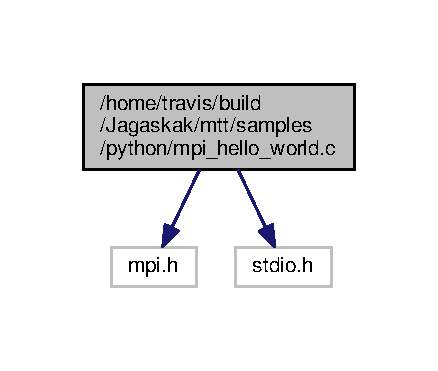
\includegraphics[width=210pt]{mpi__hello__world_8c__incl}
\end{center}
\end{figure}
\subsection*{Functions}
\begin{DoxyCompactItemize}
\item 
int \hyperlink{mpi__hello__world_8c_a3c04138a5bfe5d72780bb7e82a18e627}{main} (int argc, char $\ast$$\ast$argv)
\end{DoxyCompactItemize}


\subsection{Function Documentation}
\hypertarget{mpi__hello__world_8c_a3c04138a5bfe5d72780bb7e82a18e627}{\index{mpi\-\_\-hello\-\_\-world.\-c@{mpi\-\_\-hello\-\_\-world.\-c}!main@{main}}
\index{main@{main}!mpi_hello_world.c@{mpi\-\_\-hello\-\_\-world.\-c}}
\subsubsection[{main}]{\setlength{\rightskip}{0pt plus 5cm}int main (
\begin{DoxyParamCaption}
\item[{int}]{argc, }
\item[{char $\ast$$\ast$}]{argv}
\end{DoxyParamCaption}
)}}\label{mpi__hello__world_8c_a3c04138a5bfe5d72780bb7e82a18e627}


Definition at line 4 of file mpi\-\_\-hello\-\_\-world.\-c.


\hypertarget{mpitest_8ini}{\section{/home/travis/build/\-Jagaskak/mtt/samples/python/mpitest.ini File Reference}
\label{mpitest_8ini}\index{/home/travis/build/\-Jagaskak/mtt/samples/python/mpitest.\-ini@{/home/travis/build/\-Jagaskak/mtt/samples/python/mpitest.\-ini}}
}
\subsection*{Namespaces}
\begin{DoxyCompactItemize}
\item 
\hyperlink{namespacempitest}{mpitest}
\end{DoxyCompactItemize}

\hypertarget{ompi__hello__world_8ini}{\section{/home/travis/build/\-Jagaskak/mtt/samples/python/ompi\-\_\-hello\-\_\-world.ini File Reference}
\label{ompi__hello__world_8ini}\index{/home/travis/build/\-Jagaskak/mtt/samples/python/ompi\-\_\-hello\-\_\-world.\-ini@{/home/travis/build/\-Jagaskak/mtt/samples/python/ompi\-\_\-hello\-\_\-world.\-ini}}
}
\subsection*{Namespaces}
\begin{DoxyCompactItemize}
\item 
\hyperlink{namespaceompi__hello__world}{ompi\-\_\-hello\-\_\-world}
\end{DoxyCompactItemize}
\subsection*{Variables}
\begin{DoxyCompactItemize}
\item 
\hyperlink{namespaceompi__hello__world_a52b9c10821e333fe5c7413d414abeb1b}{ompi\-\_\-hello\-\_\-world.\-description} = M\-P\-Ihelloworld
\item 
\hyperlink{namespaceompi__hello__world_af8ab2503d0ec334a65a72e930a24e713}{ompi\-\_\-hello\-\_\-world.\-platform} = pluto
\item 
\hyperlink{namespaceompi__hello__world_a687eab84563b30840a200bfaf5407f51}{ompi\-\_\-hello\-\_\-world.\-plugin} = Git
\item 
\hyperlink{namespaceompi__hello__world_ae0dcf6cc43abc8d11428686639a5059a}{ompi\-\_\-hello\-\_\-world.\-url} = https\-://github.\-com/open-\/mpi/ompi
\item 
int \hyperlink{namespaceompi__hello__world_a34c1b9feb533b831fb7b0cd036494718}{ompi\-\_\-hello\-\_\-world.\-branch} = v1.\-10
\item 
\hyperlink{namespaceompi__hello__world_a5508612e06f3402554fdda7a9eca7d62}{ompi\-\_\-hello\-\_\-world.\-parent} = Middleware\-Get\-:\-O\-M\-P\-I
\item 
\hyperlink{namespaceompi__hello__world_ab26bf3479d404017c9d0623f42e9dcd3}{ompi\-\_\-hello\-\_\-world.\-autogen\-\_\-cmd} = ./autogen.\-pl
\item 
\hyperlink{namespaceompi__hello__world_a7b6bd890daea8a06c3daea5019b415f1}{ompi\-\_\-hello\-\_\-world.\-configure\-\_\-options} =
\item 
int \hyperlink{namespaceompi__hello__world_a3b1603e3acde68a17311cb93a6a5ef12}{ompi\-\_\-hello\-\_\-world.\-make\-\_\-options} = -\/j10
\item 
\hyperlink{namespaceompi__hello__world_a89cf2df98bd1f53501da343b4a25846c}{ompi\-\_\-hello\-\_\-world.\-src} = /opt/mtt/samples/python/
\item 
\hyperlink{namespaceompi__hello__world_a64807561a94c3ff5b1c9a945e580f643}{ompi\-\_\-hello\-\_\-world.\-middleware} = Middleware\-Build\-:\-O\-M\-P\-I
\item 
\hyperlink{namespaceompi__hello__world_a8e605d382654baee6320ca445c211c82}{ompi\-\_\-hello\-\_\-world.\-command} = mpiccmpi\-\_\-hello\-\_\-world.\-c-\/ompi\-\_\-hello\-\_\-world
\item 
\hyperlink{namespaceompi__hello__world_a6aa613720eb4f4129d00b6469b68d7cf}{ompi\-\_\-hello\-\_\-world.\-job\-\_\-name} = M\-T\-T\-\_\-\-T\-E\-S\-T
\item 
int \hyperlink{namespaceompi__hello__world_a4bc86d53822edfbcb8b35e8fc40d0075}{ompi\-\_\-hello\-\_\-world.\-options} = -\/N4
\item 
\hyperlink{namespaceompi__hello__world_a7df798e8beb69ae3bf2537c25e7b7370}{ompi\-\_\-hello\-\_\-world.\-test\-\_\-list} = mpi\-\_\-hello\-\_\-world
\item 
\hyperlink{namespaceompi__hello__world_ae42ce8011012447dba87c7337e9ddab8}{ompi\-\_\-hello\-\_\-world.\-filename} = ompi\-\_\-hello\-\_\-world.\-xml
\end{DoxyCompactItemize}

\hypertarget{ompi__snapshot__seq_8ini}{\section{/home/travis/build/\-Jagaskak/mtt/samples/python/ompi\-\_\-snapshot\-\_\-seq.ini File Reference}
\label{ompi__snapshot__seq_8ini}\index{/home/travis/build/\-Jagaskak/mtt/samples/python/ompi\-\_\-snapshot\-\_\-seq.\-ini@{/home/travis/build/\-Jagaskak/mtt/samples/python/ompi\-\_\-snapshot\-\_\-seq.\-ini}}
}
\subsection*{Namespaces}
\begin{DoxyCompactItemize}
\item 
\hyperlink{namespaceompi__snapshot__seq}{ompi\-\_\-snapshot\-\_\-seq}
\end{DoxyCompactItemize}
\subsection*{Variables}
\begin{DoxyCompactItemize}
\item 
\hyperlink{namespaceompi__snapshot__seq_a10070286ec527c9dfed8c210ca3917d7}{ompi\-\_\-snapshot\-\_\-seq.\-trial} = false
\item 
\hyperlink{namespaceompi__snapshot__seq_a8855b0a58b147479b623ede37dab8378}{ompi\-\_\-snapshot\-\_\-seq.\-scratch} = R\-E\-P\-L\-A\-C\-E\-\_\-\-M\-E\-\_\-\-P\-A\-T\-H\-\_\-\-T\-O\-\_\-\-S\-C\-R\-A\-T\-C\-H\-\_\-\-D\-I\-R
\item 
\hyperlink{namespaceompi__snapshot__seq_a918891e52aa1a572f039326981585a7a}{ompi\-\_\-snapshot\-\_\-seq.\-description} = Open\-M\-P\-Imaster
\item 
\hyperlink{namespaceompi__snapshot__seq_a300d0cc664225df572aad2518569d7bf}{ompi\-\_\-snapshot\-\_\-seq.\-platform} = R\-E\-P\-L\-A\-C\-E\-\_\-\-M\-E
\item 
\hyperlink{namespaceompi__snapshot__seq_a6293c71d0991763a4bad8b010e0e6ce2}{ompi\-\_\-snapshot\-\_\-seq.\-executor} = sequential
\item 
\hyperlink{namespaceompi__snapshot__seq_a4964274b9eb87e06a95ee1bef66604ef}{ompi\-\_\-snapshot\-\_\-seq.\-plugin} = O\-M\-P\-I\-\_\-\-Snapshot
\item 
\hyperlink{namespaceompi__snapshot__seq_a0af6b7793981b72fee25ffd1d077fd86}{ompi\-\_\-snapshot\-\_\-seq.\-url} = https\-://download.\-open-\/mpi.\-org/nightly/open-\/mpi/master
\item 
\hyperlink{namespaceompi__snapshot__seq_ab1bd70042bbcbfc640abba12010ed2b5}{ompi\-\_\-snapshot\-\_\-seq.\-version\-\_\-file} = R\-E\-P\-L\-A\-C\-E\-\_\-\-M\-E\-\_\-\-N\-A\-M\-E\-\_\-\-O\-F\-\_\-\-V\-E\-R\-S\-I\-O\-N\-\_\-\-F\-I\-L\-E
\item 
\hyperlink{namespaceompi__snapshot__seq_a464fbb2313394347fa064032378c5674}{ompi\-\_\-snapshot\-\_\-seq.\-mpi\-\_\-name} = ompi-\/nightly-\/master
\item 
\hyperlink{namespaceompi__snapshot__seq_a08a86b12770df9f65150ce521c8820b6}{ompi\-\_\-snapshot\-\_\-seq.\-parent} = Middleware\-Get\-:\-O\-M\-P\-I\-Master
\item 
\hyperlink{namespaceompi__snapshot__seq_affb396ef384900a98c5a943dd8817711}{ompi\-\_\-snapshot\-\_\-seq.\-configure\-\_\-options} = -\/-\/enable-\/debug
\item 
int \hyperlink{namespaceompi__snapshot__seq_a42ad6d7d01611e1404c4747596bad26f}{ompi\-\_\-snapshot\-\_\-seq.\-make\-\_\-options} = -\/j1
\item 
\hyperlink{namespaceompi__snapshot__seq_a9d517656629849b65e1dcefbcf9cfd73}{ompi\-\_\-snapshot\-\_\-seq.\-subdir} = ibm
\item 
int \hyperlink{namespaceompi__snapshot__seq_ad98d5c78e44526c2b86baccb081cd46e}{ompi\-\_\-snapshot\-\_\-seq.\-merge\-\_\-stdout\-\_\-stderr} = 1
\item 
int \hyperlink{namespaceompi__snapshot__seq_a4c1170c00e6cc51822262da67c07d721}{ompi\-\_\-snapshot\-\_\-seq.\-stderr\-\_\-save\-\_\-lines} = 100
\item 
\hyperlink{namespaceompi__snapshot__seq_a25acb4b0e7bb13ac146f46ae7f074689}{ompi\-\_\-snapshot\-\_\-seq.\-middleware} = Middleware\-Build\-:\-O\-M\-P\-I\-Master
\item 
\hyperlink{namespaceompi__snapshot__seq_a2e5939b3a3bd4bacecb7b4b33cad0313}{ompi\-\_\-snapshot\-\_\-seq.\-autogen\-\_\-cmd} = ./autogen.\-sh
\item 
\hyperlink{namespaceompi__snapshot__seq_a7ee776e6bd84fc7f42f758751ba25e1e}{ompi\-\_\-snapshot\-\_\-seq.\-command} = mpirun
\item 
int \hyperlink{namespaceompi__snapshot__seq_ac5c6ca602093f9742f1afbfc100f8cfd}{ompi\-\_\-snapshot\-\_\-seq.\-np} = 2
\item 
int \hyperlink{namespaceompi__snapshot__seq_a7261e8a10955a8c08df3d642714fb626}{ompi\-\_\-snapshot\-\_\-seq.\-skipped} = 77
\item 
int \hyperlink{namespaceompi__snapshot__seq_a0521277c015b3e1b74418fc58101d5d6}{ompi\-\_\-snapshot\-\_\-seq.\-stdout\-\_\-save\-\_\-lines} = 100
\item 
int \hyperlink{namespaceompi__snapshot__seq_a4a2554fd9d8c0df86eeaae67f5bc6867}{ompi\-\_\-snapshot\-\_\-seq.\-timeout} = 600
\item 
string \hyperlink{namespaceompi__snapshot__seq_ae15b0abc55bc72ce7a7a4ebe56fc2dfe}{ompi\-\_\-snapshot\-\_\-seq.\-test\-\_\-dir} = \char`\"{}collective, communicator, datatype, environment, group, info, io, onesided, pt2pt, random, topology\char`\"{}
\item 
int \hyperlink{namespaceompi__snapshot__seq_a8c173774cc05394e996dbb13e37d0322}{ompi\-\_\-snapshot\-\_\-seq.\-max\-\_\-num\-\_\-tests} = 10
\item 
string \hyperlink{namespaceompi__snapshot__seq_a1c6caf43d8724d112db736b1cc590bef}{ompi\-\_\-snapshot\-\_\-seq.\-fail\-\_\-tests} = \char`\"{}environment/abort, environment/final\char`\"{}
\item 
\hyperlink{namespaceompi__snapshot__seq_ac68ac424f71d3b098f0e5742e90083c1}{ompi\-\_\-snapshot\-\_\-seq.\-fail\-\_\-timeout} = max\-\_\-procs
\item 
string \hyperlink{namespaceompi__snapshot__seq_a0a1e6182d0b6b408fd0b3642c5b52556}{ompi\-\_\-snapshot\-\_\-seq.\-skip\-\_\-tests} = \char`\"{}environment/init\-\_\-thread\-\_\-multiple,communicator/comm\-\_\-split\-\_\-f\char`\"{}
\item 
\hyperlink{namespaceompi__snapshot__seq_ac375b04988441d39d7dbd8546bede172}{ompi\-\_\-snapshot\-\_\-seq.\-filename} = mttresults.\-txt
\item 
\hyperlink{namespaceompi__snapshot__seq_ae564d5d2ad344e6edd9fe25c04553c4f}{ompi\-\_\-snapshot\-\_\-seq.\-summary\-\_\-footer} =
\item 
\hyperlink{namespaceompi__snapshot__seq_aa8131df6b7e79ce54a5832a78a18226b}{ompi\-\_\-snapshot\-\_\-seq.\-detail\-\_\-header} =
\item 
\hyperlink{namespaceompi__snapshot__seq_a0238cbbb945d76de96b90e3cd058d356}{ompi\-\_\-snapshot\-\_\-seq.\-detail\-\_\-footer} =
\item 
int \hyperlink{namespaceompi__snapshot__seq_a81239e350a24a25aa3a329f330a267f4}{ompi\-\_\-snapshot\-\_\-seq.\-textwrap} = 78
\item 
\hyperlink{namespaceompi__snapshot__seq_aab43e86098df5461b6d69d6554bacf51}{ompi\-\_\-snapshot\-\_\-seq.\-realm} = O\-M\-P\-I
\item 
\hyperlink{namespaceompi__snapshot__seq_ad73553bb8a0851422895d9c7e8978b83}{ompi\-\_\-snapshot\-\_\-seq.\-username} = R\-E\-P\-L\-A\-C\-E\-\_\-\-M\-E
\item 
\hyperlink{namespaceompi__snapshot__seq_a6229810db63f8ab2e0598c9dc5da7a32}{ompi\-\_\-snapshot\-\_\-seq.\-password} = R\-E\-P\-L\-A\-C\-E\-\_\-\-M\-E
\end{DoxyCompactItemize}

\hypertarget{test_8ini}{\section{/home/travis/build/\-Jagaskak/mtt/samples/python/test.ini File Reference}
\label{test_8ini}\index{/home/travis/build/\-Jagaskak/mtt/samples/python/test.\-ini@{/home/travis/build/\-Jagaskak/mtt/samples/python/test.\-ini}}
}
\subsection*{Namespaces}
\begin{DoxyCompactItemize}
\item 
\hyperlink{namespacetest}{test}
\end{DoxyCompactItemize}
\subsection*{Variables}
\begin{DoxyCompactItemize}
\item 
int \hyperlink{namespacetest_ad4773f49ae244cf1cfa3fe9cbbce0d67}{test.\-force} = 1
\item 
int \hyperlink{namespacetest_a0e85c866c38cad5d7ae36d1115224da0}{test.\-trial} = 0
\item 
\hyperlink{namespacetest_aab6125cbc3654cbeb0f5df11bf28b3f1}{test.\-scratch} = /home/common/mttscratch-\/rsh
\item 
int \hyperlink{namespacetest_afa4c185ba5d92fdbefba5736ef442945}{test.\-submit\-\_\-group\-\_\-results} = 1
\item 
\hyperlink{namespacetest_ad95cf6979c5decba613e5a1d5ffe07a7}{test.\-logfile} = /home/common/mtt-\/logfile-\/rsh.\-txt
\item 
\hyperlink{namespacetest_a1c2a3a63faa9854257983fbb3de9e11d}{test.\-description} = Prototypetestconfigurationfile
\item 
\hyperlink{namespacetest_ac5ddc75d7029ace1bfb95e457e5c3510}{test.\-name} = My\-Installation
\item 
\hyperlink{namespacetest_ab75fa7ca9f0cb2bcac8a454434a9f2ed}{test.\-module} = Already\-Installed
\item 
\hyperlink{namespacetest_aa7f544791c7eba91f19e926b661617a1}{test.\-hostfile} = /home/common/hosts
\item 
\hyperlink{namespacetest_a306f9d9d5c20138c75077ea9bb2b2df4}{test.\-exec} = mpirun
\item 
tuple \hyperlink{namespacetest_abc155792ba7b2057124cc069e596899f}{test.\-pass} = \&and(\&cmd\-\_\-wifexited(), \&eq(\&cmd\-\_\-wexitstatus(), 0))
\item 
tuple \hyperlink{namespacetest_a7a09931cf523b8af2e201bee605f000c}{test.\-skipped} = \&and(\&test\-\_\-wifexited(), \&eq(\&test\-\_\-wexitstatus(), 77))
\item 
int \hyperlink{namespacetest_ad6c2143462bf99c62dcb7cf691a56394}{test.\-save\-\_\-stdout\-\_\-on\-\_\-pass} = 1
\item 
int \hyperlink{namespacetest_ab42f6c72b039645ef575cfb31b7b99e8}{test.\-merge\-\_\-stdout\-\_\-stderr} = 1
\item 
int \hyperlink{namespacetest_ad4c8d1b4c04f99668eb1f7168aee5dec}{test.\-stdout\-\_\-save\-\_\-lines} = 100
\item 
int \hyperlink{namespacetest_a6eb3ee4197f9fe28682af6f06cbc5e8f}{test.\-stderr\-\_\-save\-\_\-lines} = 100
\item 
int \hyperlink{namespacetest_a86e28e32de6c6c5e79ed64d05f513b97}{test.\-report\-\_\-after\-\_\-n\-\_\-results} = 100
\item 
int \hyperlink{namespacetest_a1535a7960a63eaf5e78bb6685abd44e8}{test.\-np} = 16
\item 
\hyperlink{namespacetest_a9c562b60dd319bbf228d80c2285c3fde}{test.\-scm\-\_\-module} = Git
\item 
\hyperlink{namespacetest_a6eab9a211bdeacabe249075b1612c3d9}{test.\-scm\-\_\-url} = /home/common/ompi-\/tests
\item 
\hyperlink{namespacetest_a954686f4e1dc4fd9b53353f75443c6a1}{test.\-scm\-\_\-subdir} = ibm
\item 
string \hyperlink{namespacetest_a96c17bd039b26da494c806d745289285}{test.\-pre\-\_\-config\-\_\-cmd} = \char`\"{}./autogen.\-sh\char`\"{}
\item 
\hyperlink{namespacetest_aed30062928699cb82ebdc01629cc1ec2}{test.\-test\-\_\-get} = trivial
\item 
int \hyperlink{namespacetest_a222c8f53a587af9263d043662a13938b}{test.\-save\-\_\-stdout\-\_\-on\-\_\-success} = 1
\item 
\hyperlink{namespacetest_a567f95611fb12515b764d829ae44aabb}{test.\-target\-\_\-install} = My\-Installation
\item 
string \hyperlink{namespacetest_a94ef7b9eb439fa68dbcb5ffd2b3247d2}{test.\-config\-\_\-cmd} = \char`\"{}./configure C\-C=mpicc C\-X\-X=mpic++ F77=mpif77\char`\"{}
\item 
string \hyperlink{namespacetest_aaa8f1db02a6b0b450565529cebd91d5c}{test.\-build\-\_\-cmd} = \char`\"{}make -\/j 10\char`\"{}
\item 
\hyperlink{namespacetest_a295e67a63678237853b86e59182db440}{test.\-mpi\-\_\-install} = My\-Installation
\item 
\hyperlink{namespacetest_ae4fd57c0f20abaa78ea8f6e1a2dd6625}{test.\-intel\-\_\-ompi\-\_\-tests\-\_\-buildfile} = all\-\_\-tests\-\_\-no\-\_\-perf
\item 
\hyperlink{namespacetest_aec036affe0d08e5c43462900a6548769}{test.\-test\-\_\-build} = Trivial
\item 
tuple \hyperlink{namespacetest_a69079090d6416ccf53f5c565fa229a77}{test.\-timeout} = max(10, np)
\item 
string \hyperlink{namespacetest_a8ff2dd5a1198312fe9ada87a755956ab}{test.\-find\-\_\-test\-\_\-dir} = \char`\"{}.\char`\"{}
\item 
string \hyperlink{namespacetest_ae0ea3fdd2b6f2c8c3bb11f0afc20a097}{test.\-fail\-\_\-tests} = \char`\"{}environment/abort, environment/final\char`\"{}
\item 
\hyperlink{namespacetest_abfd7a3bf875f29c0fe5342e1345eef93}{test.\-fail\-\_\-timeout} = max\-\_\-procs
\item 
string \hyperlink{namespacetest_a92bc9c8909f4ebfd33da729397fa6669}{test.\-skip\-\_\-tests} = \char`\"{}environment/init\-\_\-thread\-\_\-multiple,communicator/comm\-\_\-split\-\_\-f\char`\"{}
\item 
\hyperlink{namespacetest_ab8d549258085b48d9a6ab8be50b86939}{test.\-include\-\_\-section} = Testrun
\item 
\hyperlink{namespacetest_a51dc8620c2e0770b19a7478de3cdfe9f}{test.\-specify\-\_\-module} = Simple
\item 
\hyperlink{namespacetest_a710122d20448f56ed2401cc3aa94ba04}{test.\-mttdatabase\-\_\-realm} = O\-M\-P\-I
\item 
\hyperlink{namespacetest_a7097267c4c5626a8f8e3376be40a9a92}{test.\-mttdatabase\-\_\-username} = intel
\item 
tuple \hyperlink{namespacetest_a51e535ad16f2253bc9fa6509c258a110}{test.\-mttdatabase\-\_\-password} = \&stringify(\&cat(\char`\"{}/home/common/mttpwd.\-txt\char`\"{}))
\item 
\hyperlink{namespacetest_ad84ae15a19ed5e82248ae54549e3d0d9}{test.\-mttdatabase\-\_\-platform} = bend-\/rsh
\item 
tuple \hyperlink{namespacetest_ade0bfe5e5627318e781e4d494c889bd3}{test.\-mttdatabase\-\_\-hostname} = \&env\-\_\-hosts()
\item 
\hyperlink{namespacetest_ad3dde693468cd5e08314bbab4c9f58ef}{test.\-mttdatabase\-\_\-url} = https\-://mtt.\-open-\/mpi.\-org/submit/
\item 
\hyperlink{namespacetest_ad8091a4ab1a4450f8e8c7039d81bbd92}{test.\-mttdatabase\-\_\-debug\-\_\-filename} = mttdb\-\_\-debug\-\_\-file
\item 
int \hyperlink{namespacetest_a9a41a6defd3632956b1fe345985788f6}{test.\-mttdatabase\-\_\-keep\-\_\-debug\-\_\-files} = 1
\item 
int \hyperlink{namespacetest_a3ac6ed984e10925873b601b7c08e0a17}{test.\-mttdatabase\-\_\-debug\-\_\-server} = 1
\item 
\hyperlink{namespacetest_a39cdd407082b44f6d5bf56c03b99a745}{test.\-textfile\-\_\-filename} = \$phase-\/\$section-\/\$mpi\-\_\-name-\/\$mpi\-\_\-version.\-txt
\item 
\hyperlink{namespacetest_a9cf6c35d175b44931bbc0e7ee120ba6d}{test.\-textfile\-\_\-summary\-\_\-footer} =
\item 
\hyperlink{namespacetest_a1149fe2728a88b0d33fdd5606ce953b2}{test.\-textfile\-\_\-detail\-\_\-header} =
\item 
\hyperlink{namespacetest_a26400b6c12ab57d038c2ecc468f19645}{test.\-textfile\-\_\-detail\-\_\-footer} =
\item 
int \hyperlink{namespacetest_a8f79316c7cc4b1d1ed80e5dbb71a8249}{test.\-textfile\-\_\-textwrap} = 78
\end{DoxyCompactItemize}

%--- End generated contents ---

% Index
\newpage
\phantomsection
\addcontentsline{toc}{chapter}{Index}
\printindex

\end{document}
